% !TeX program = xelatex
% !TeX encoding = UTF-8
% Presentazione revisionata: Futura: previsione e progetto statistico
% Basata sul materiale originale fornito dall'autore e sul template M01_Pensare_con_i_dati.tex
% Compilazione: xelatex -interaction=nonstopmode Futura_M10_previsione_progetto.tex (due passaggi)
% Diagrammi TikZ e figure statistiche vettoriali; sorgenti R e dati inclusi.
% Revisione completa delle 110 slide; fonti consultate il 20 novembre 2026.
\documentclass[12pt,aspectratio=1610]{beamer}
\geometry{paperwidth=20cm,paperheight=12.5cm}
\usepackage[italian,provide=*]{babel}
\usepackage{fontspec}
\IfFontExistsTF{NimbusSans-Regular.otf}{
\setsansfont{NimbusSans-Regular.otf}[BoldFont=NimbusSans-Bold.otf,ItalicFont=NimbusSans-Italic.otf,BoldItalicFont=NimbusSans-BoldItalic.otf]
\setmainfont{NimbusSans-Regular.otf}[BoldFont=NimbusSans-Bold.otf,ItalicFont=NimbusSans-Italic.otf,BoldItalicFont=NimbusSans-BoldItalic.otf]
}{
\setsansfont{TeX Gyre Heros}
\setmainfont{TeX Gyre Heros}
}
\IfFontExistsTF{DejaVu Sans Mono}{
\setmonofont{DejaVu Sans Mono}[Scale=.88]
}{\setmonofont{Latin Modern Mono}[Scale=.88]}
\usefonttheme{professionalfonts}
\usepackage{amsmath,amssymb,booktabs,array,graphicx,tikz,bookmark}
\usetikzlibrary{calc,positioning,arrows.meta}
\graphicspath{{Risorse/Figure/}}
\definecolor{Paper}{HTML}{F8F6F1}
\definecolor{Ink}{HTML}{253344}
\definecolor{Navy}{HTML}{15283E}
\definecolor{Quantum}{HTML}{5146A5}
\definecolor{Classical}{HTML}{087C74}
\definecolor{Muted}{HTML}{657180}
\definecolor{Rule}{HTML}{D6DAD9}
\definecolor{Night}{HTML}{112236}
\definecolor{Lilac}{HTML}{ABB5FF}
\definecolor{Mint}{HTML}{72D8C8}
\setbeamercolor{background canvas}{bg=Paper}
\setbeamercolor{normal text}{fg=Ink}
\setbeamertemplate{navigation symbols}{}
\setbeamertemplate{headline}{}
\setbeamertemplate{footline}{}
\setbeamersize{text margin left=0pt,text margin right=0pt}
\hypersetup{colorlinks=true,linkcolor=Classical,urlcolor=Classical,pdfpagemode=UseOutlines,pdfstartview=Fit,
 pdftitle={Futura: previsione e progetto statistico},pdfauthor={Marzio De Corato},
 pdfsubject={Modulo M10: previsione, valutazione temporale e progetto statistico, Revisione completa: diagrammi TikZ, formule e codice R commentato}}
\bookmarksetup{open,openlevel=0,depth=2}
\newsavebox{\BodyBox}
\newsavebox{\SideBox}
\newsavebox{\RecallBox}
\newsavebox{\TitleBox}
\newcommand{\MeasureBox}[2]{\typeout{REVIEWBOX:#1:\the\wd#2:\the\ht#2:\the\dp#2}}

% Revisione completa: diagrammi TikZ, formalismo e box R.
\usepackage[most]{tcolorbox}
\usepackage{listings}
\usetikzlibrary{fit,backgrounds,matrix,decorations.pathreplacing}
\definecolor{GeoA}{HTML}{1D7890}
\definecolor{GeoB}{HTML}{C57E42}
\definecolor{GeoC}{HTML}{7363AA}
\definecolor{GeoTint}{HTML}{F0F4F3}
\lstdefinestyle{GeoR}{language=R,basicstyle=\ttfamily\fontsize{9.2}{12.2}\selectfont,
 keywordstyle=\color{Quantum}\bfseries,commentstyle=\color{Classical},stringstyle=\color{GeoB},
 numbers=left,numberstyle=\tiny\color{Muted},numbersep=4pt,showstringspaces=false,
 columns=fullflexible,keepspaces=true,breaklines=true,xleftmargin=1.15em,
 frame=none,aboveskip=0pt,belowskip=0pt,tabsize=2}
\newsavebox{\PilotLeftBox}
\newsavebox{\PilotRightBox}
\newcommand{\PLabel}[1]{\par{\color{Classical}\bfseries\fontsize{9}{11}\selectfont\MakeUppercase{#1}}\par\vspace{1.8mm}}
\newcommand{\PBody}[1]{\par{\fontsize{11.3}{14.8}\selectfont #1\par}}
\newcommand{\PSmall}[1]{\par{\fontsize{9.8}{13.1}\selectfont #1\par}}
\newcommand{\PCode}[2]{%
\begin{tcolorbox}[enhanced,arc=1.8mm,boxrule=.65pt,
  colback=white,colframe=Classical!75!Navy,colbacktitle=Navy,
  coltitle=white,fonttitle=\bfseries\fontsize{9.6}{12}\selectfont,
  title={#1},left=1.7mm,right=1.3mm,top=1.5mm,bottom=1.3mm,
  before skip=1mm,after skip=1mm]
\lstinputlisting[style=GeoR]{Codice/#2}
\end{tcolorbox}}
\newcommand{\PInfo}[1]{%
\begin{tcolorbox}[enhanced,arc=1.6mm,boxrule=.55pt,colback=GeoTint,
 colframe=Rule!80!Classical,left=2.3mm,right=2.3mm,top=2mm,bottom=2mm,
 before skip=1mm,after skip=1mm]
\PSmall{#1}\end{tcolorbox}}
\tikzset{
 pFlow/.style={draw=Classical!45,fill=white,rounded corners=2mm,
  line width=.7pt,align=center,minimum height=1.1cm,font=\sffamily\fontsize{10}{12}\selectfont},
 pEdge/.style={-{Latex[length=2.3mm]},draw=Classical,line width=.95pt},
 pGroup/.style={draw=Rule,fill=white,rounded corners=2mm,line width=.65pt},
 pDotA/.style={circle,fill=GeoA,inner sep=1.25pt},
 pDotB/.style={circle,fill=GeoB,inner sep=1.25pt},
 pDotC/.style={circle,fill=GeoC,inner sep=1.25pt}
}
\newcommand{\PilotChrome}[4]{%
  \node[anchor=north west,inner sep=0,text width=17.7cm] at ([xshift=.95cm,yshift=-.55cm]current page.north west) {\color{Navy}\bfseries\fontsize{20.6}{24.5}\selectfont #1};
  \node[anchor=north east,inner sep=0] at ([xshift=19.05cm,yshift=-.14cm]current page.north west) {\color{Classical}\fontsize{8}{10}\selectfont\hyperlink{slide2}{#2}};
  \draw[Classical,line width=1.2pt] ([xshift=.95cm,yshift=-1.7cm]current page.north west)--([xshift=2.35cm,yshift=-1.7cm]current page.north west);
  \draw[Rule,line width=.65pt] ([xshift=.95cm,yshift=-10.36cm]current page.north west)--([xshift=19.05cm,yshift=-10.36cm]current page.north west);
  \node[anchor=north west,inner sep=0] at ([xshift=.96cm,yshift=-10.55cm]current page.north west) {\color{Classical}\bfseries\fontsize{9.1}{12}\selectfont DA RICORDARE};
  \node[anchor=north west,inner sep=0,text width=14.3cm] at ([xshift=4.2cm,yshift=-10.53cm]current page.north west) {\color{Ink}\fontsize{10.3}{13.8}\selectfont #4};
  \draw[Rule,line width=.35pt] ([xshift=.95cm,yshift=-11.92cm]current page.north west)--([xshift=19.05cm,yshift=-11.92cm]current page.north west);
  \node[anchor=north west,inner sep=0] at ([xshift=.95cm,yshift=-12.06cm]current page.north west) {\color{Muted}\fontsize{7.7}{9.2}\selectfont Futura: previsione e progetto statistico};
  \node[anchor=north east,inner sep=0] at ([xshift=19.05cm,yshift=-12.06cm]current page.north west) {\color{Muted}\fontsize{7.7}{9.2}\selectfont #3/110};
}


% Stili comuni per i diagrammi scientifici della revisione completa.
\tikzset{
 pAxis/.style={-{Latex[length=2mm]},draw=Muted,line width=.65pt},
 pNote/.style={font=\sffamily\fontsize{9}{11.5}\selectfont,text=Muted,align=center},
 pLabel/.style={font=\sffamily\fontsize{10}{12.5}\selectfont,text=Ink,align=center}
}
\newsavebox{\FullWideBox}
\setlength{\emergencystretch}{1em}




\newcommand{\PLab}[2]{\par{\color{Classical}\bfseries\fontsize{9}{11}\selectfont
\href{#1}{\MakeUppercase{#2}}}\par\vspace{1.8mm}}


\begin{document}

\begin{frame}[plain]\hypertarget{slide1}{}\bookmark[level=0,page=1]{Futura}
\begin{tikzpicture}[remember picture,overlay]
\fill[Night](current page.south west) rectangle(current page.north east);
\IfFileExists{Risorse/Copertine/M10_Futura.jpg}{\node[inner sep=0] at(current page.center){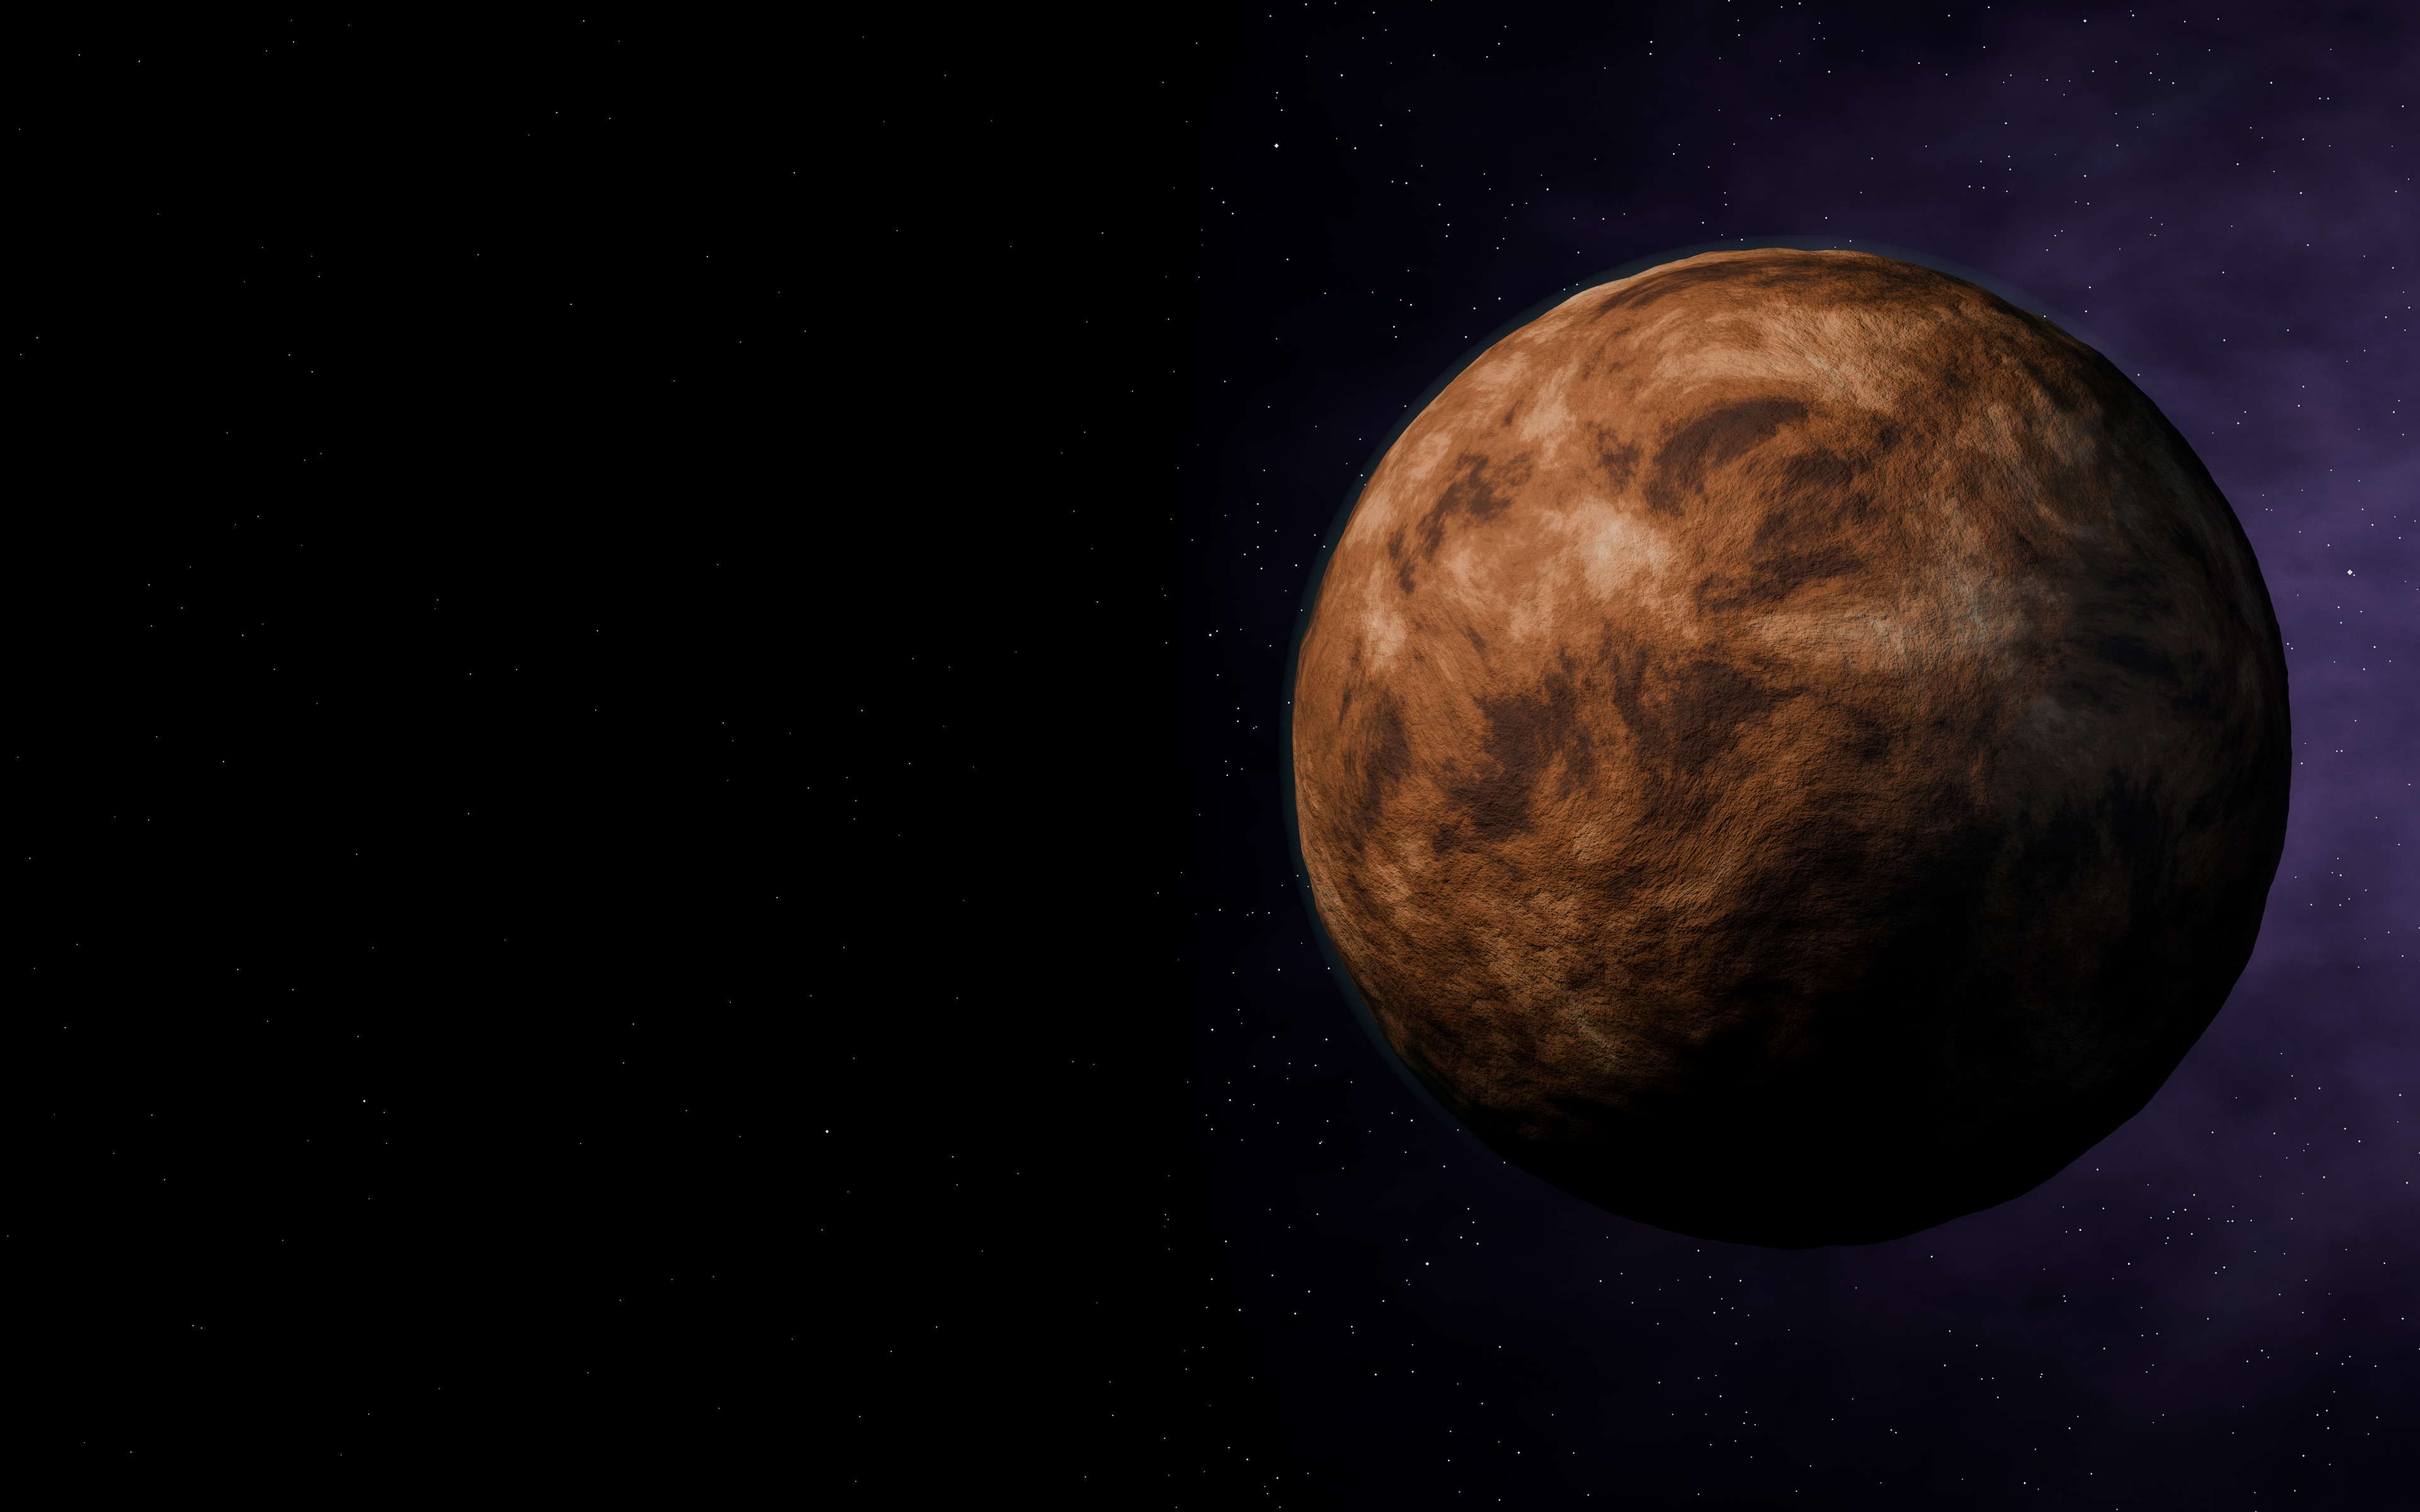
\includegraphics[width=20cm,height=12.5cm]{Risorse/Copertine/M10_Futura.jpg}};}{}
\node[anchor=north west,inner sep=0] at([xshift=1.05cm,yshift=-1.10cm]current page.north west){\color{Mint}\bfseries\fontsize{23}{28}\selectfont FUTURA};
\node[anchor=north west,inner sep=0] at([xshift=1.07cm,yshift=-2.16cm]current page.north west){\color{white}\fontsize{9}{12}\selectfont MODULO M10 · SCIENZE DELLA TERRA};
\draw[Mint,line width=1.5pt]([xshift=1.07cm,yshift=-2.78cm]current page.north west)--([xshift=2.6cm,yshift=-2.78cm]current page.north west);
\node[anchor=north west,inner sep=0] at([xshift=1.05cm,yshift=-3.35cm]current page.north west){\begin{minipage}{9.2cm}\raggedright\color{white}\bfseries\fontsize{30}{36}\selectfont Previsione\\e progetto\\statistico\end{minipage}};
\node[anchor=north west,inner sep=0] at([xshift=1.07cm,yshift=-7.88cm]current page.north west){\begin{minipage}{8.9cm}\raggedright\color{Lilac}\fontsize{12.2}{17}\selectfont Modelli temporali, valutazione\\e argomentazione scientifica\end{minipage}};
\node[anchor=north west,inner sep=0] at([xshift=1.07cm,yshift=-10.52cm]current page.north west){\color{white}\fontsize{11.5}{15}\selectfont Marzio De Corato};
\node[anchor=north west,inner sep=0] at([xshift=1.07cm,yshift=-11.17cm]current page.north west){\color{Mint}\fontsize{8.8}{11}\selectfont\href{https://creativecommons.org/licenses/by-nc-sa/4.0/}{© 2026 · CC BY-NC-SA 4.0}};
\end{tikzpicture}\end{frame}
\begin{frame}[plain]\hypertarget{slide2}{}
\bookmark[level=0,page=2]{I · IL COMPITO PREVISIONALE}
\bookmark[level=1,page=2]{Un percorso dalla domanda alla previsione}
\begin{lrbox}{\TitleBox}
\begin{minipage}[t]{17.7cm}\raggedright\color{Ink}\fontsize{11.3}{14.8}\selectfont
\color{Navy}\bfseries\fontsize{20.6}{24.5}\selectfont Un percorso dalla domanda alla previsione
\end{minipage}\end{lrbox}
\typeout{FULLBOX:002:TitleBox:\the\ht\TitleBox:\the\dp\TitleBox}

\begin{lrbox}{\RecallBox}
\begin{minipage}[t]{14.3cm}\raggedright\color{Ink}\fontsize{11.3}{14.8}\selectfont
\fontsize{10.3}{13.8}\selectfont Una buona previsione nasce da una domanda verificabile e da un protocollo dichiarato.
\end{minipage}\end{lrbox}
\typeout{FULLBOX:002:RecallBox:\the\ht\RecallBox:\the\dp\RecallBox}

\begin{lrbox}{\PilotLeftBox}
\begin{minipage}[t]{10.05cm}\raggedright\color{Ink}\fontsize{11.3}{14.8}\selectfont
\PLabel{Nove passaggi collegati}
{\fontsize{10.2}{13.1}\selectfont\renewcommand{\arraystretch}{1.45}\begin{tabular}{@{}p{8.3cm}p{0.7cm}@{}}\toprule
\textbf{Sezione} & \textbf{p.}\\\midrule
\hyperlink{slide3}{Definire il compito e l’informazione} & 3\\
\hyperlink{slide11}{Costruire riferimenti confrontabili} & 11\\
\hyperlink{slide23}{Capire memoria e innovazioni} & 23\\
\hyperlink{slide40}{Specificare ARIMA e stagionalità} & 40\\
\hyperlink{slide58}{Diagnosticare le innovazioni stimate} & 58\\
\hyperlink{slide70}{Validare rispettando il tempo} & 70\\
\hyperlink{slide83}{Leggere errori e intervalli} & 83\\
\hyperlink{slide94}{Estendere a due variabili} & 94\\
\hyperlink{slide102}{Consegnare un progetto riproducibile} & 102\\
\bottomrule\end{tabular}}

\end{minipage}\end{lrbox}
\typeout{FULLBOX:002:PilotLeftBox:\the\ht\PilotLeftBox:\the\dp\PilotLeftBox}

\begin{lrbox}{\PilotRightBox}
\begin{minipage}[t]{7.55cm}\raggedright\color{Ink}\fontsize{11.3}{14.8}\selectfont
\PBody{Borealis ha introdotto calendario, dipendenza e trasformazioni. Futura usa queste conoscenze per formulare e valutare una previsione.}
\vspace{2.5mm}
\PInfo{Tre archivi locali: CO$_2$ storica, fossili simulati e processi temporali simulati. Ogni risultato conserva unità, periodo e origine.}
\PBody{Le 20 attività mantengono gli identificativi M10\_N01--M10\_N20 del sito. I notebook aggiungono risultati eseguiti, spiegazioni e verifiche.}
\vspace{2.5mm}

\end{minipage}\end{lrbox}
\typeout{FULLBOX:002:PilotRightBox:\the\ht\PilotRightBox:\the\dp\PilotRightBox}

\begin{tikzpicture}[remember picture,overlay]
\PilotChrome{Un percorso dalla domanda alla previsione}{I · IL COMPITO PREVISIONALE}{2}{Una buona previsione nasce da una domanda verificabile e da un protocollo dichiarato.}
\node[anchor=north west,inner sep=0] at([xshift=.96cm,yshift=-2.13cm]current page.north west){\usebox{\PilotLeftBox}};
\node[anchor=north west,inner sep=0] at([xshift=11.52cm,yshift=-2.13cm]current page.north west){\usebox{\PilotRightBox}};
\end{tikzpicture}\end{frame}

\begin{frame}[plain]\hypertarget{slide3}{}
\bookmark[level=1,page=3]{Dal descrivere una serie al prevederne il seguito}
\begin{lrbox}{\TitleBox}
\begin{minipage}[t]{17.7cm}\raggedright\color{Ink}\fontsize{11.3}{14.8}\selectfont
\color{Navy}\bfseries\fontsize{20.6}{24.5}\selectfont Dal descrivere una serie al prevederne il seguito
\end{minipage}\end{lrbox}
\typeout{FULLBOX:003:TitleBox:\the\ht\TitleBox:\the\dp\TitleBox}

\begin{lrbox}{\RecallBox}
\begin{minipage}[t]{14.3cm}\raggedright\color{Ink}\fontsize{11.3}{14.8}\selectfont
\fontsize{10.3}{13.8}\selectfont L’adeguatezza descrittiva e l’utilità previsionale rispondono a domande diverse.
\end{minipage}\end{lrbox}
\typeout{FULLBOX:003:RecallBox:\the\ht\RecallBox:\the\dp\RecallBox}

\begin{lrbox}{\PilotLeftBox}
\begin{minipage}[t]{10.05cm}\raggedright\color{Ink}\fontsize{11.3}{14.8}\selectfont
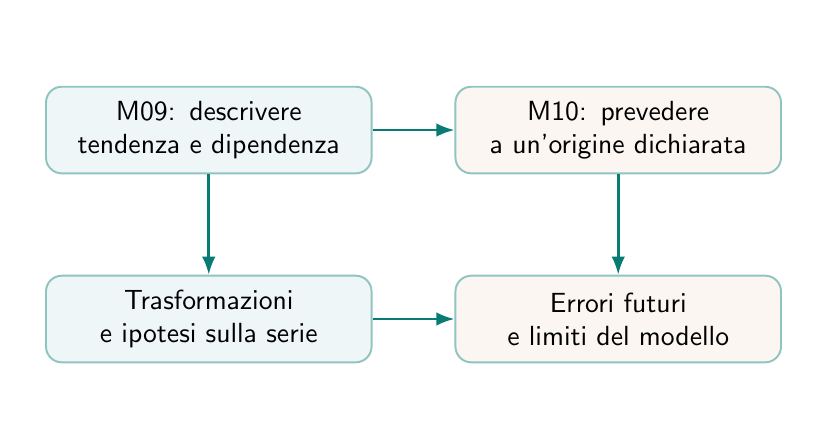
\begin{tikzpicture}[x=1cm,y=1cm]
\path[use as bounding box](-.1,-.15) rectangle(9.7,4.8);
\node[pFlow,text width=3.9cm,fill=GeoA!7] (a) at(2.2,3.5){M09: descrivere\\tendenza e dipendenza};
\node[pFlow,text width=3.9cm,fill=GeoB!7] (b) at(7.4,3.5){M10: prevedere\\a un’origine dichiarata};
\node[pFlow,text width=3.9cm,fill=GeoA!7] (c) at(2.2,1.1){Trasformazioni\\e ipotesi sulla serie};
\node[pFlow,text width=3.9cm,fill=GeoB!7] (d) at(7.4,1.1){Errori futuri\\e limiti del modello};
\draw[pEdge] (a) -- (b);
\draw[pEdge] (a) -- (c);
\draw[pEdge] (b) -- (d);
\draw[pEdge] (c) -- (d);
\end{tikzpicture}
\[\{y_1,\ldots,y_T\}\quad\longrightarrow\quad\widehat y_{T+h\mid T}\]

\end{minipage}\end{lrbox}
\typeout{FULLBOX:003:PilotLeftBox:\the\ht\PilotLeftBox:\the\dp\PilotLeftBox}

\begin{lrbox}{\PilotRightBox}
\begin{minipage}[t]{7.55cm}\raggedright\color{Ink}\fontsize{11.3}{14.8}\selectfont
\PBody{La descrizione riguarda ciò che osserviamo. La previsione aggiunge un criterio: il modello deve funzionare su valori che non ha usato per stimarsi.}
\vspace{2.5mm}
\PInfo{Riconoscere una stagione non garantisce che la previsione migliori un semplice ciclo ripetuto.}
\PBody{Il caso guida è una verifica storica: ci collochiamo a dicembre 1998 e valutiamo i mesi successivi.}
\vspace{2.5mm}

\end{minipage}\end{lrbox}
\typeout{FULLBOX:003:PilotRightBox:\the\ht\PilotRightBox:\the\dp\PilotRightBox}

\begin{tikzpicture}[remember picture,overlay]
\PilotChrome{Dal descrivere una serie al prevederne il seguito}{I · IL COMPITO PREVISIONALE}{3}{L’adeguatezza descrittiva e l’utilità previsionale rispondono a domande diverse.}
\node[anchor=north west,inner sep=0] at([xshift=.96cm,yshift=-2.13cm]current page.north west){\usebox{\PilotLeftBox}};
\node[anchor=north west,inner sep=0] at([xshift=11.52cm,yshift=-2.13cm]current page.north west){\usebox{\PilotRightBox}};
\end{tikzpicture}\end{frame}

\begin{frame}[plain]\hypertarget{slide4}{}
\bookmark[level=1,page=4]{Origine, orizzonte e variabile da prevedere}
\begin{lrbox}{\TitleBox}
\begin{minipage}[t]{17.7cm}\raggedright\color{Ink}\fontsize{11.3}{14.8}\selectfont
\color{Navy}\bfseries\fontsize{20.6}{24.5}\selectfont Origine, orizzonte e variabile da prevedere
\end{minipage}\end{lrbox}
\typeout{FULLBOX:004:TitleBox:\the\ht\TitleBox:\the\dp\TitleBox}

\begin{lrbox}{\RecallBox}
\begin{minipage}[t]{14.3cm}\raggedright\color{Ink}\fontsize{11.3}{14.8}\selectfont
\fontsize{10.3}{13.8}\selectfont Ogni previsione deve indicare che cosa prevede, quando viene emessa e quanto lontano guarda.
\end{minipage}\end{lrbox}
\typeout{FULLBOX:004:RecallBox:\the\ht\RecallBox:\the\dp\RecallBox}

\begin{lrbox}{\PilotLeftBox}
\begin{minipage}[t]{10.05cm}\raggedright\color{Ink}\fontsize{11.3}{14.8}\selectfont
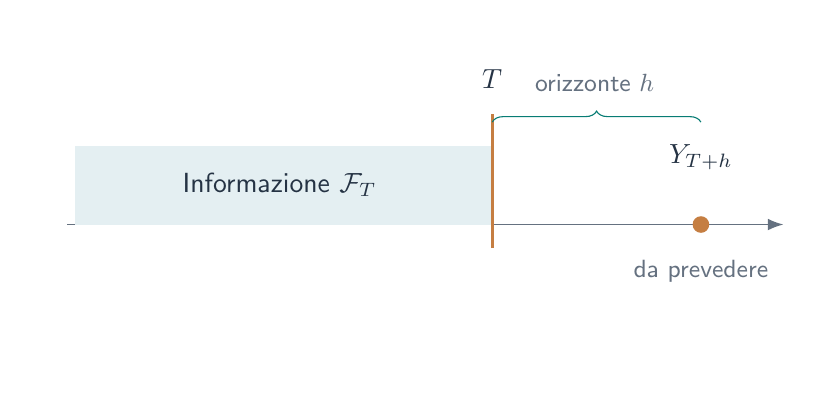
\begin{tikzpicture}[x=1cm,y=1cm]
\path[use as bounding box](-.1,-.15) rectangle(9.7,4.2);
\draw[pAxis](.4,1.7)--(9.5,1.7);
\fill[GeoA!12](.5,1.7)rectangle(5.8,2.7);
\node[pLabel]at(3.1,2.2){Informazione $\mathcal F_T$};
\draw[GeoB,line width=1.2pt](5.8,1.4)--(5.8,3.1);
\node[pLabel]at(5.8,3.55){$T$};
\fill[GeoB](8.45,1.7)circle(3pt);
\node[pLabel]at(8.45,2.55){$Y_{T+h}$};
\node[pNote]at(8.45,1.1){da prevedere};
\draw[decorate,decoration={brace,amplitude=4pt},Classical](5.8,3.0)--(8.45,3.0);
\node[pNote]at(7.1,3.5){orizzonte $h$};
\end{tikzpicture}
\[\widehat y_{T+h\mid T}=g_h(\mathcal F_T)\]

\end{minipage}\end{lrbox}
\typeout{FULLBOX:004:PilotLeftBox:\the\ht\PilotLeftBox:\the\dp\PilotLeftBox}

\begin{lrbox}{\PilotRightBox}
\begin{minipage}[t]{7.55cm}\raggedright\color{Ink}\fontsize{11.3}{14.8}\selectfont
\PBody{L’origine $T$ è l’ultimo istante con dati disponibili. L’orizzonte $h$ misura la distanza fino al valore futuro. La variabile deve avere unità e risoluzione esplicite.}
\vspace{2.5mm}
\PInfo{Qui: concentrazione media mensile derivata di CO$_2$, in ppm. Origine dicembre 1998; orizzonti da 1 a 36 mesi.}
\PCode{R · fissare origine e orizzonte}{004_esempio.R}
\end{minipage}\end{lrbox}
\typeout{FULLBOX:004:PilotRightBox:\the\ht\PilotRightBox:\the\dp\PilotRightBox}

\begin{tikzpicture}[remember picture,overlay]
\PilotChrome{Origine, orizzonte e variabile da prevedere}{I · IL COMPITO PREVISIONALE}{4}{Ogni previsione deve indicare che cosa prevede, quando viene emessa e quanto lontano guarda.}
\node[anchor=north west,inner sep=0] at([xshift=.96cm,yshift=-2.13cm]current page.north west){\usebox{\PilotLeftBox}};
\node[anchor=north west,inner sep=0] at([xshift=11.52cm,yshift=-2.13cm]current page.north west){\usebox{\PilotRightBox}};
\node[anchor=north east,inner sep=0] at([xshift=17.65cm,yshift=-12.06cm]current page.north west){\color{Classical}\fontsize{7.7}{9.2}\selectfont\href{../../03_Notebook_svolti/M10_Futura/M10_N01.html}{M10\_N01 · notebook svolto}};
\end{tikzpicture}\end{frame}

\begin{frame}[plain]\hypertarget{slide5}{}
\bookmark[level=1,page=5]{Quali informazioni esistono davvero all’origine?}
\begin{lrbox}{\TitleBox}
\begin{minipage}[t]{17.7cm}\raggedright\color{Ink}\fontsize{11.3}{14.8}\selectfont
\color{Navy}\bfseries\fontsize{20.6}{24.5}\selectfont Quali informazioni esistono davvero all’origine?
\end{minipage}\end{lrbox}
\typeout{FULLBOX:005:TitleBox:\the\ht\TitleBox:\the\dp\TitleBox}

\begin{lrbox}{\RecallBox}
\begin{minipage}[t]{14.3cm}\raggedright\color{Ink}\fontsize{11.3}{14.8}\selectfont
\fontsize{10.3}{13.8}\selectfont La disponibilità dell’informazione è una proprietà del compito, non della colonna nel file.
\end{minipage}\end{lrbox}
\typeout{FULLBOX:005:RecallBox:\the\ht\RecallBox:\the\dp\RecallBox}

\begin{lrbox}{\PilotLeftBox}
\begin{minipage}[t]{10.05cm}\raggedright\color{Ink}\fontsize{11.3}{14.8}\selectfont
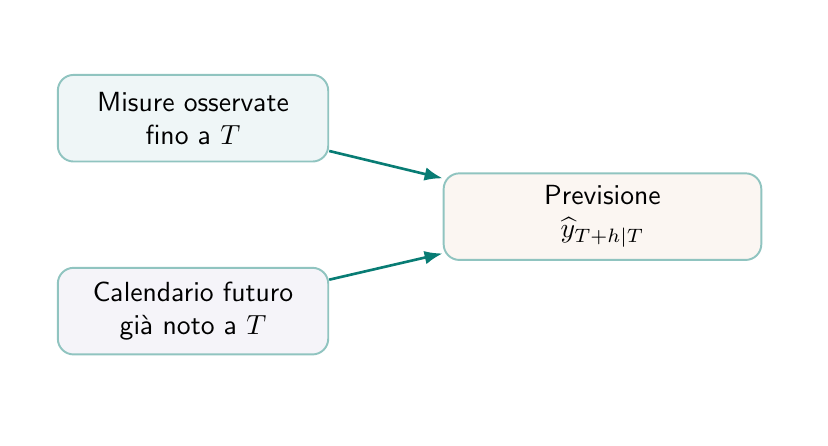
\begin{tikzpicture}[x=1cm,y=1cm]
\path[use as bounding box](-.1,-.15) rectangle(9.7,4.8);
\node[pFlow,text width=3.2cm,fill=GeoA!7] (a) at(2.0,3.65){Misure osservate\\fino a $T$};
\node[pFlow,text width=3.2cm,fill=GeoC!7] (b) at(2.0,1.2){Calendario futuro\\già noto a $T$};
\node[pFlow,text width=3.8cm,fill=GeoB!7] (c) at(7.2,2.4){Previsione\\$\widehat y_{T+h\mid T}$};
\draw[pEdge] (a) -- (c);
\draw[pEdge] (b) -- (c);
\end{tikzpicture}
\PSmall{La misura futura entra soltanto quando si valuta l’errore.}

\end{minipage}\end{lrbox}
\typeout{FULLBOX:005:PilotLeftBox:\the\ht\PilotLeftBox:\the\dp\PilotLeftBox}

\begin{lrbox}{\PilotRightBox}
\begin{minipage}[t]{7.55cm}\raggedright\color{Ink}\fontsize{11.3}{14.8}\selectfont
\PBody{Il mese dell’anno è noto in anticipo. Una temperatura futura misurata sul campo non lo è. Un regressore utilizzabile in stima può quindi non essere disponibile in previsione.}
\vspace{2.5mm}
\PInfo{Per covariate future ignote occorre prevederle, definire scenari o rinunciare al loro impiego. La scelta va dichiarata nel compito.}
\PBody{Anche correzioni, medie mobili e normalizzazioni devono usare soltanto l’informazione accessibile all’origine.}
\vspace{2.5mm}

\end{minipage}\end{lrbox}
\typeout{FULLBOX:005:PilotRightBox:\the\ht\PilotRightBox:\the\dp\PilotRightBox}

\begin{tikzpicture}[remember picture,overlay]
\PilotChrome{Quali informazioni esistono davvero all’origine?}{I · IL COMPITO PREVISIONALE}{5}{La disponibilità dell’informazione è una proprietà del compito, non della colonna nel file.}
\node[anchor=north west,inner sep=0] at([xshift=.96cm,yshift=-2.13cm]current page.north west){\usebox{\PilotLeftBox}};
\node[anchor=north west,inner sep=0] at([xshift=11.52cm,yshift=-2.13cm]current page.north west){\usebox{\PilotRightBox}};
\end{tikzpicture}\end{frame}

\begin{frame}[plain]\hypertarget{slide6}{}
\bookmark[level=1,page=6]{Un protocollo storico con date precise}
\begin{lrbox}{\TitleBox}
\begin{minipage}[t]{17.7cm}\raggedright\color{Ink}\fontsize{11.3}{14.8}\selectfont
\color{Navy}\bfseries\fontsize{20.6}{24.5}\selectfont Un protocollo storico con date precise
\end{minipage}\end{lrbox}
\typeout{FULLBOX:006:TitleBox:\the\ht\TitleBox:\the\dp\TitleBox}

\begin{lrbox}{\RecallBox}
\begin{minipage}[t]{14.3cm}\raggedright\color{Ink}\fontsize{11.3}{14.8}\selectfont
\fontsize{10.3}{13.8}\selectfont Il test finale valuta una procedura già definita; non serve a scegliere la variante più favorevole.
\end{minipage}\end{lrbox}
\typeout{FULLBOX:006:RecallBox:\the\ht\RecallBox:\the\dp\RecallBox}

\begin{lrbox}{\PilotLeftBox}
\begin{minipage}[t]{10.05cm}\raggedright\color{Ink}\fontsize{11.3}{14.8}\selectfont
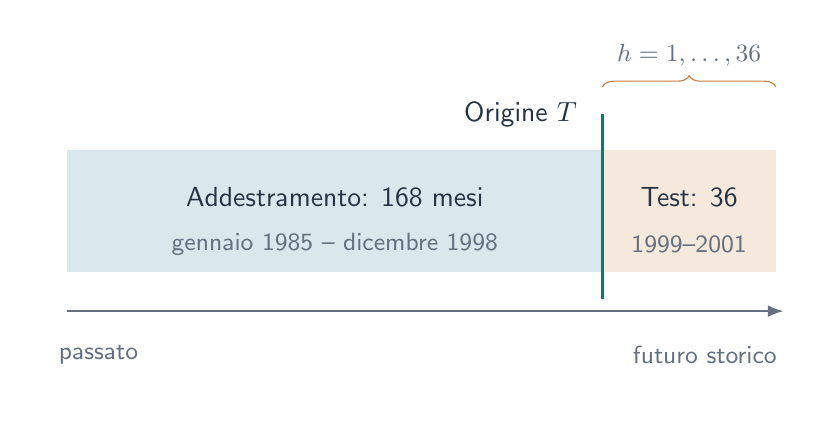
\begin{tikzpicture}[x=1cm,y=1cm]
\path[use as bounding box](-.1,-.15) rectangle(9.7,4.8);
\fill[GeoA!17](.4,1.7)rectangle(7.2,3.25);
\fill[GeoB!18](7.2,1.7)rectangle(9.4,3.25);
\node[pLabel]at(3.8,2.65){Addestramento: 168 mesi};
\node[pNote]at(3.8,2.05){gennaio 1985 -- dicembre 1998};
\node[pLabel]at(8.3,2.65){Test: 36};
\node[pNote]at(8.3,2.05){1999--2001};
\draw[Classical,line width=1pt](7.2,1.35)--(7.2,3.7);
\node[pLabel,anchor=east]at(7.0,3.7){Origine $T$};
\draw[pAxis](.4,1.2)--(9.5,1.2);
\node[pNote]at(.8,.65){passato};\node[pNote]at(8.5,.65){futuro storico};
\draw[decorate,decoration={brace,amplitude=4pt},GeoB](7.2,4.05)--(9.4,4.05);
\node[pNote]at(8.3,4.45){$h=1,\ldots,36$};
\end{tikzpicture}
{\fontsize{10.2}{13.1}\selectfont\renewcommand{\arraystretch}{1.45}\begin{tabular}{@{}p{3cm}p{6.1cm}@{}}\toprule
\textbf{Parte} & \textbf{Uso}\\\midrule
1985--1998 & Stima, diagnostica, validazione interna\\
1999--2001 & Verifica finale del protocollo fissato\\
\bottomrule\end{tabular}}

\end{minipage}\end{lrbox}
\typeout{FULLBOX:006:PilotLeftBox:\the\ht\PilotLeftBox:\the\dp\PilotLeftBox}

\begin{lrbox}{\PilotRightBox}
\begin{minipage}[t]{7.55cm}\raggedright\color{Ink}\fontsize{11.3}{14.8}\selectfont
\PBody{La separazione viene fissata prima di confrontare i risultati sul test. I 168 mesi iniziali contengono tutte le informazioni usate per stimare il modello.}
\vspace{2.5mm}
\PInfo{Le tre origini interne sono dicembre 1994, 1995 e 1996; ciascuna prevede i 12 mesi successivi, sempre dentro il periodo di addestramento.}
\PCode{R · separare per calendario}{006_esempio.R}
\end{minipage}\end{lrbox}
\typeout{FULLBOX:006:PilotRightBox:\the\ht\PilotRightBox:\the\dp\PilotRightBox}

\begin{tikzpicture}[remember picture,overlay]
\PilotChrome{Un protocollo storico con date precise}{I · IL COMPITO PREVISIONALE}{6}{Il test finale valuta una procedura già definita; non serve a scegliere la variante più favorevole.}
\node[anchor=north west,inner sep=0] at([xshift=.96cm,yshift=-2.13cm]current page.north west){\usebox{\PilotLeftBox}};
\node[anchor=north west,inner sep=0] at([xshift=11.52cm,yshift=-2.13cm]current page.north west){\usebox{\PilotRightBox}};
\node[anchor=north east,inner sep=0] at([xshift=17.65cm,yshift=-12.06cm]current page.north west){\color{Classical}\fontsize{7.7}{9.2}\selectfont\href{../../03_Notebook_svolti/M10_Futura/M10_N01.html}{M10\_N01 · notebook svolto}};
\end{tikzpicture}\end{frame}

\begin{frame}[plain]\hypertarget{slide7}{}
\bookmark[level=1,page=7]{La CO2 è un archivio storico documentato}
\begin{lrbox}{\TitleBox}
\begin{minipage}[t]{17.7cm}\raggedright\color{Ink}\fontsize{11.3}{14.8}\selectfont
\color{Navy}\bfseries\fontsize{20.6}{24.5}\selectfont La CO2 è un archivio storico documentato
\end{minipage}\end{lrbox}
\typeout{FULLBOX:007:TitleBox:\the\ht\TitleBox:\the\dp\TitleBox}

\begin{lrbox}{\RecallBox}
\begin{minipage}[t]{14.3cm}\raggedright\color{Ink}\fontsize{11.3}{14.8}\selectfont
\fontsize{10.3}{13.8}\selectfont Una serie storica chiusa permette un esperimento riproducibile; la sua provenienza resta parte del risultato.
\end{minipage}\end{lrbox}
\typeout{FULLBOX:007:RecallBox:\the\ht\RecallBox:\the\dp\RecallBox}

\begin{lrbox}{\PilotLeftBox}
\begin{minipage}[t]{10.05cm}\raggedright\color{Ink}\fontsize{11.3}{14.8}\selectfont
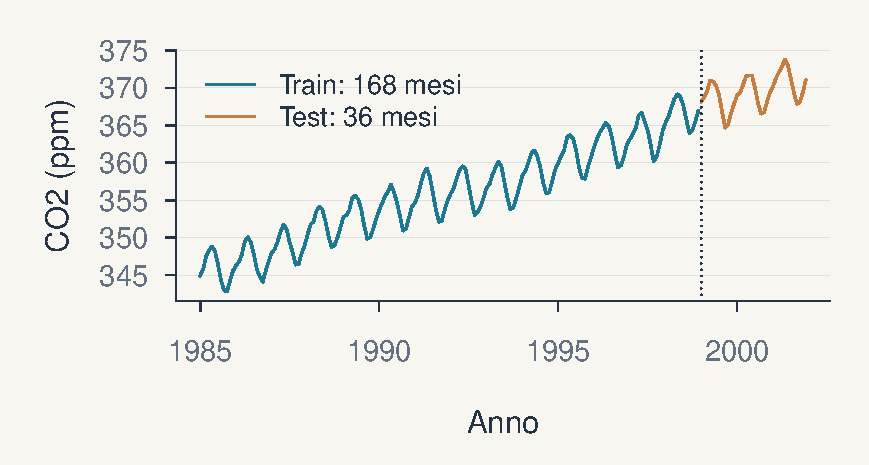
\includegraphics[width=9.85cm,height=5.25cm,keepaspectratio]{Risultati/Figure/01_CO2_finestra.pdf}
\vspace{1.5mm}
\PSmall{204 medie mensili derivate; separazione a dicembre 1998. I dati terminano nel 2001.}

\end{minipage}\end{lrbox}
\typeout{FULLBOX:007:PilotLeftBox:\the\ht\PilotLeftBox:\the\dp\PilotLeftBox}

\begin{lrbox}{\PilotRightBox}
\begin{minipage}[t]{7.55cm}\raggedright\color{Ink}\fontsize{11.3}{14.8}\selectfont
\PBody{Il file locale riprende la serie di M09. Le medie mensili derivano dall’aggregazione dei valori settimanali del vecchio archivio distribuito con statsmodels.}
\vspace{2.5mm}
\PInfo{La data associata al mese e il numero di settimane disponibili restano nel CSV. Questa aggregazione non coincide necessariamente con una serie mensile ufficiale.}
\PSmall{La provenienza e l’impronta SHA-256 sono conservate con i dati. Il notebook non scarica nuovi valori durante l’esecuzione.}

\end{minipage}\end{lrbox}
\typeout{FULLBOX:007:PilotRightBox:\the\ht\PilotRightBox:\the\dp\PilotRightBox}

\begin{tikzpicture}[remember picture,overlay]
\PilotChrome{La CO2 è un archivio storico documentato}{I · IL COMPITO PREVISIONALE}{7}{Una serie storica chiusa permette un esperimento riproducibile; la sua provenienza resta parte del risultato.}
\node[anchor=north west,inner sep=0] at([xshift=.96cm,yshift=-2.13cm]current page.north west){\usebox{\PilotLeftBox}};
\node[anchor=north west,inner sep=0] at([xshift=11.52cm,yshift=-2.13cm]current page.north west){\usebox{\PilotRightBox}};
\end{tikzpicture}\end{frame}

\begin{frame}[plain]\hypertarget{slide8}{}
\bookmark[level=1,page=8]{Prevedere una distribuzione futura}
\begin{lrbox}{\TitleBox}
\begin{minipage}[t]{17.7cm}\raggedright\color{Ink}\fontsize{11.3}{14.8}\selectfont
\color{Navy}\bfseries\fontsize{20.6}{24.5}\selectfont Prevedere una distribuzione futura
\end{minipage}\end{lrbox}
\typeout{FULLBOX:008:TitleBox:\the\ht\TitleBox:\the\dp\TitleBox}

\begin{lrbox}{\RecallBox}
\begin{minipage}[t]{14.3cm}\raggedright\color{Ink}\fontsize{11.3}{14.8}\selectfont
\fontsize{10.3}{13.8}\selectfont Centro, dispersione e probabilità degli eventi devono essere interpretati separatamente.
\end{minipage}\end{lrbox}
\typeout{FULLBOX:008:RecallBox:\the\ht\RecallBox:\the\dp\RecallBox}

\begin{lrbox}{\PilotLeftBox}
\begin{minipage}[t]{10.05cm}\raggedright\color{Ink}\fontsize{11.3}{14.8}\selectfont
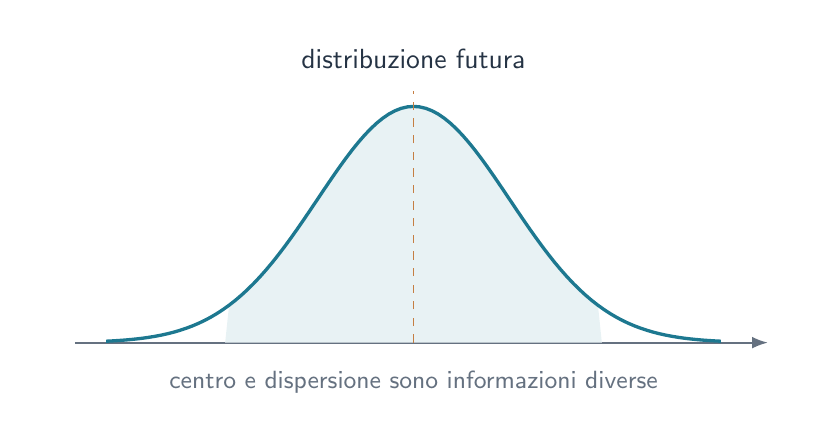
\begin{tikzpicture}[x=1cm,y=1cm]
\path[use as bounding box](-.1,-.15) rectangle(9.7,4.8);
\draw[pAxis](.5,.8)--(9.3,.8);\fill[GeoA!10](2.408,.8)--(2.4576,1.2749) -- (2.5357,1.3359) -- (2.6138,1.4023) -- (2.6918,1.4741) -- (2.7699,1.5514) -- (2.8480,1.6341) -- (2.9261,1.7222) -- (3.0042,1.8153) -- (3.0822,1.9134) -- (3.1603,2.0159) -- (3.2384,2.1224) -- (3.3165,2.2323) -- (3.3946,2.3451) -- (3.4726,2.4599) -- (3.5507,2.5759) -- (3.6288,2.6923) -- (3.7069,2.8081) -- (3.7850,2.9223) -- (3.8630,3.0338) -- (3.9411,3.1415) -- (4.0192,3.2444) -- (4.0973,3.3414) -- (4.1754,3.4315) -- (4.2534,3.5136) -- (4.3315,3.5868) -- (4.4096,3.6503) -- (4.4877,3.7033) -- (4.5658,3.7452) -- (4.6438,3.7755) -- (4.7219,3.7939) -- (4.8000,3.8000) -- (4.8781,3.7939) -- (4.9562,3.7755) -- (5.0342,3.7452) -- (5.1123,3.7033) -- (5.1904,3.6503) -- (5.2685,3.5868) -- (5.3466,3.5136) -- (5.4246,3.4315) -- (5.5027,3.3414) -- (5.5808,3.2444) -- (5.6589,3.1415) -- (5.7370,3.0338) -- (5.8150,2.9223) -- (5.8931,2.8081) -- (5.9712,2.6923) -- (6.0493,2.5759) -- (6.1274,2.4599) -- (6.2054,2.3451) -- (6.2835,2.2323) -- (6.3616,2.1224) -- (6.4397,2.0159) -- (6.5178,1.9134) -- (6.5958,1.8153) -- (6.6739,1.7222) -- (6.7520,1.6341) -- (6.8301,1.5514) -- (6.9082,1.4741) -- (6.9862,1.4023) -- (7.0643,1.3359) -- (7.1424,1.2749)--(7.192,.8)--cycle;\draw[GeoA,line width=1.2pt]plot coordinates{(0.8960,0.8179) (0.9741,0.8220) (1.0522,0.8268) (1.1302,0.8325) (1.2083,0.8394) (1.2864,0.8474) (1.3645,0.8569) (1.4426,0.8680) (1.5206,0.8809) (1.5987,0.8959) (1.6768,0.9132) (1.7549,0.9331) (1.8330,0.9559) (1.9110,0.9818) (1.9891,1.0111) (2.0672,1.0441) (2.1453,1.0811) (2.2234,1.1225) (2.3014,1.1684) (2.3795,1.2192) (2.4576,1.2749) (2.5357,1.3359) (2.6138,1.4023) (2.6918,1.4741) (2.7699,1.5514) (2.8480,1.6341) (2.9261,1.7222) (3.0042,1.8153) (3.0822,1.9134) (3.1603,2.0159) (3.2384,2.1224) (3.3165,2.2323) (3.3946,2.3451) (3.4726,2.4599) (3.5507,2.5759) (3.6288,2.6923) (3.7069,2.8081) (3.7850,2.9223) (3.8630,3.0338) (3.9411,3.1415) (4.0192,3.2444) (4.0973,3.3414) (4.1754,3.4315) (4.2534,3.5136) (4.3315,3.5868) (4.4096,3.6503) (4.4877,3.7033) (4.5658,3.7452) (4.6438,3.7755) (4.7219,3.7939) (4.8000,3.8000) (4.8781,3.7939) (4.9562,3.7755) (5.0342,3.7452) (5.1123,3.7033) (5.1904,3.6503) (5.2685,3.5868) (5.3466,3.5136) (5.4246,3.4315) (5.5027,3.3414) (5.5808,3.2444) (5.6589,3.1415) (5.7370,3.0338) (5.8150,2.9223) (5.8931,2.8081) (5.9712,2.6923) (6.0493,2.5759) (6.1274,2.4599) (6.2054,2.3451) (6.2835,2.2323) (6.3616,2.1224) (6.4397,2.0159) (6.5178,1.9134) (6.5958,1.8153) (6.6739,1.7222) (6.7520,1.6341) (6.8301,1.5514) (6.9082,1.4741) (6.9862,1.4023) (7.0643,1.3359) (7.1424,1.2749) (7.2205,1.2192) (7.2986,1.1684) (7.3766,1.1225) (7.4547,1.0811) (7.5328,1.0441) (7.6109,1.0111) (7.6890,0.9818) (7.7670,0.9559) (7.8451,0.9331) (7.9232,0.9132) (8.0013,0.8959) (8.0794,0.8809) (8.1574,0.8680) (8.2355,0.8569) (8.3136,0.8474) (8.3917,0.8394) (8.4698,0.8325) (8.5478,0.8268) (8.6259,0.8220) (8.7040,0.8179)};\draw[GeoB,dashed](4.8,.8)--(4.8,4.0);\node[pLabel]at(4.8,4.4){distribuzione futura};\node[pNote]at(4.8,.3){centro e dispersione sono informazioni diverse};
\end{tikzpicture}
\[Y_{T+h}\mid\mathcal F_T\ \sim\ F_{T,h}\]

\end{minipage}\end{lrbox}
\typeout{FULLBOX:008:PilotLeftBox:\the\ht\PilotLeftBox:\the\dp\PilotLeftBox}

\begin{lrbox}{\PilotRightBox}
\begin{minipage}[t]{7.55cm}\raggedright\color{Ink}\fontsize{11.3}{14.8}\selectfont
\PBody{La previsione puntuale riassume la distribuzione futura. L’intervallo descrive parte della sua dispersione, condizionatamente alle ipotesi adottate.}
\vspace{2.5mm}
\PInfo{Due modelli possono avere lo stesso centro e attribuire probabilità molto diverse ai valori estremi.}
\PBody{Un intervallo predittivo riguarda una nuova osservazione. Un intervallo per la media descrive l’incertezza di una quantità media e risponde a un’altra domanda.}
\vspace{2.5mm}

\end{minipage}\end{lrbox}
\typeout{FULLBOX:008:PilotRightBox:\the\ht\PilotRightBox:\the\dp\PilotRightBox}

\begin{tikzpicture}[remember picture,overlay]
\PilotChrome{Prevedere una distribuzione futura}{I · IL COMPITO PREVISIONALE}{8}{Centro, dispersione e probabilità degli eventi devono essere interpretati separatamente.}
\node[anchor=north west,inner sep=0] at([xshift=.96cm,yshift=-2.13cm]current page.north west){\usebox{\PilotLeftBox}};
\node[anchor=north west,inner sep=0] at([xshift=11.52cm,yshift=-2.13cm]current page.north west){\usebox{\PilotRightBox}};
\end{tikzpicture}\end{frame}

\begin{frame}[plain]\hypertarget{slide9}{}
\bookmark[level=1,page=9]{La perdita stabilisce quale centro è ottimale}
\begin{lrbox}{\TitleBox}
\begin{minipage}[t]{17.7cm}\raggedright\color{Ink}\fontsize{11.3}{14.8}\selectfont
\color{Navy}\bfseries\fontsize{20.6}{24.5}\selectfont La perdita stabilisce quale centro è ottimale
\end{minipage}\end{lrbox}
\typeout{FULLBOX:009:TitleBox:\the\ht\TitleBox:\the\dp\TitleBox}

\begin{lrbox}{\RecallBox}
\begin{minipage}[t]{14.3cm}\raggedright\color{Ink}\fontsize{11.3}{14.8}\selectfont
\fontsize{10.3}{13.8}\selectfont La previsione “migliore” dipende anche dalla perdita con cui la si valuta.
\end{minipage}\end{lrbox}
\typeout{FULLBOX:009:RecallBox:\the\ht\RecallBox:\the\dp\RecallBox}

\begin{lrbox}{\PilotLeftBox}
\begin{minipage}[t]{10.05cm}\raggedright\color{Ink}\fontsize{11.3}{14.8}\selectfont
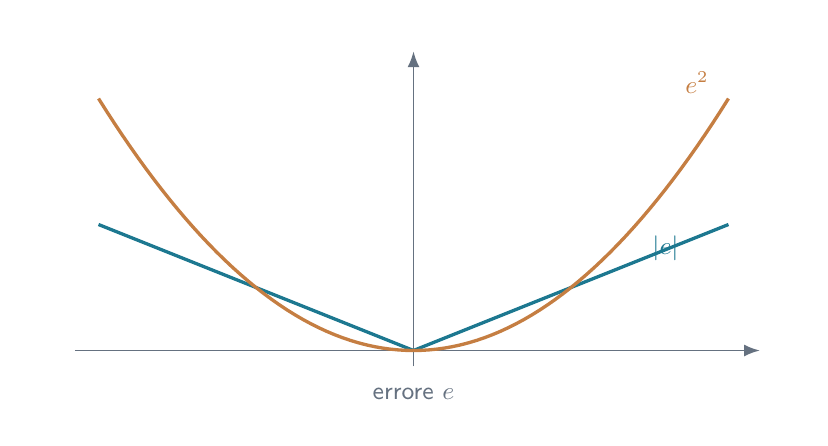
\begin{tikzpicture}[x=1cm,y=1cm]
\path[use as bounding box](-.1,-.15) rectangle(9.7,4.8);
\draw[pAxis](.5,.7)--(9.2,.7);\draw[pAxis](4.8,.5)--(4.8,4.5);
\draw[GeoA,line width=1.2pt]plot coordinates{(0.800,2.300) (0.900,2.260) (1.000,2.220) (1.100,2.180) (1.200,2.140) (1.300,2.100) (1.400,2.060) (1.500,2.020) (1.600,1.980) (1.700,1.940) (1.800,1.900) (1.900,1.860) (2.000,1.820) (2.100,1.780) (2.200,1.740) (2.300,1.700) (2.400,1.660) (2.500,1.620) (2.600,1.580) (2.700,1.540) (2.800,1.500) (2.900,1.460) (3.000,1.420) (3.100,1.380) (3.200,1.340) (3.300,1.300) (3.400,1.260) (3.500,1.220) (3.600,1.180) (3.700,1.140) (3.800,1.100) (3.900,1.060) (4.000,1.020) (4.100,0.980) (4.200,0.940) (4.300,0.900) (4.400,0.860) (4.500,0.820) (4.600,0.780) (4.700,0.740) (4.800,0.700) (4.900,0.740) (5.000,0.780) (5.100,0.820) (5.200,0.860) (5.300,0.900) (5.400,0.940) (5.500,0.980) (5.600,1.020) (5.700,1.060) (5.800,1.100) (5.900,1.140) (6.000,1.180) (6.100,1.220) (6.200,1.260) (6.300,1.300) (6.400,1.340) (6.500,1.380) (6.600,1.420) (6.700,1.460) (6.800,1.500) (6.900,1.540) (7.000,1.580) (7.100,1.620) (7.200,1.660) (7.300,1.700) (7.400,1.740) (7.500,1.780) (7.600,1.820) (7.700,1.860) (7.800,1.900) (7.900,1.940) (8.000,1.980) (8.100,2.020) (8.200,2.060) (8.300,2.100) (8.400,2.140) (8.500,2.180) (8.600,2.220) (8.700,2.260) (8.800,2.300)};
\draw[GeoB,line width=1.2pt]plot coordinates{(0.800,3.900) (0.900,3.742) (1.000,3.588) (1.100,3.438) (1.200,3.292) (1.300,3.150) (1.400,3.012) (1.500,2.878) (1.600,2.748) (1.700,2.622) (1.800,2.500) (1.900,2.382) (2.000,2.268) (2.100,2.158) (2.200,2.052) (2.300,1.950) (2.400,1.852) (2.500,1.758) (2.600,1.668) (2.700,1.582) (2.800,1.500) (2.900,1.422) (3.000,1.348) (3.100,1.278) (3.200,1.212) (3.300,1.150) (3.400,1.092) (3.500,1.038) (3.600,0.988) (3.700,0.942) (3.800,0.900) (3.900,0.862) (4.000,0.828) (4.100,0.798) (4.200,0.772) (4.300,0.750) (4.400,0.732) (4.500,0.718) (4.600,0.708) (4.700,0.702) (4.800,0.700) (4.900,0.702) (5.000,0.708) (5.100,0.718) (5.200,0.732) (5.300,0.750) (5.400,0.772) (5.500,0.798) (5.600,0.828) (5.700,0.862) (5.800,0.900) (5.900,0.942) (6.000,0.988) (6.100,1.038) (6.200,1.092) (6.300,1.150) (6.400,1.212) (6.500,1.278) (6.600,1.348) (6.700,1.422) (6.800,1.500) (6.900,1.582) (7.000,1.668) (7.100,1.758) (7.200,1.852) (7.300,1.950) (7.400,2.052) (7.500,2.158) (7.600,2.268) (7.700,2.382) (7.800,2.500) (7.900,2.622) (8.000,2.748) (8.100,2.878) (8.200,3.012) (8.300,3.150) (8.400,3.292) (8.500,3.438) (8.600,3.588) (8.700,3.742) (8.800,3.900)};
\node[pNote,text=GeoA]at(8,2.0){$|e|$};\node[pNote,text=GeoB]at(8.4,4.1){$e^2$};
\node[pNote]at(4.8,.15){errore $e$};
\end{tikzpicture}
\[\arg\min_a\,\mathbb E[(Y-a)^2\mid\mathcal F_T]=\mathbb E[Y\mid\mathcal F_T]\]

\end{minipage}\end{lrbox}
\typeout{FULLBOX:009:PilotLeftBox:\the\ht\PilotLeftBox:\the\dp\PilotLeftBox}

\begin{lrbox}{\PilotRightBox}
\begin{minipage}[t]{7.55cm}\raggedright\color{Ink}\fontsize{11.3}{14.8}\selectfont
\PBody{La perdita quadratica penalizza fortemente gli errori grandi e porta alla media condizionata. Con perdita assoluta, una mediana condizionata minimizza il rischio.}
\vspace{2.5mm}
\PInfo{Perdite asimmetriche possono favorire un quantile: sottostimare e sovrastimare non hanno sempre lo stesso costo.}
\PSmall{Nel modulo useremo MAE e RMSE, dichiarando anche il segno dell’errore. Un’unica graduatoria non rappresenta ogni possibile decisione.}

\end{minipage}\end{lrbox}
\typeout{FULLBOX:009:PilotRightBox:\the\ht\PilotRightBox:\the\dp\PilotRightBox}

\begin{tikzpicture}[remember picture,overlay]
\PilotChrome{La perdita stabilisce quale centro è ottimale}{I · IL COMPITO PREVISIONALE}{9}{La previsione “migliore” dipende anche dalla perdita con cui la si valuta.}
\node[anchor=north west,inner sep=0] at([xshift=.96cm,yshift=-2.13cm]current page.north west){\usebox{\PilotLeftBox}};
\node[anchor=north west,inner sep=0] at([xshift=11.52cm,yshift=-2.13cm]current page.north west){\usebox{\PilotRightBox}};
\end{tikzpicture}\end{frame}

\begin{frame}[plain]\hypertarget{slide10}{}
\bookmark[level=1,page=10]{Il quaderno del compito previsionale}
\begin{lrbox}{\TitleBox}
\begin{minipage}[t]{17.7cm}\raggedright\color{Ink}\fontsize{11.3}{14.8}\selectfont
\color{Navy}\bfseries\fontsize{20.6}{24.5}\selectfont Il quaderno del compito previsionale
\end{minipage}\end{lrbox}
\typeout{FULLBOX:010:TitleBox:\the\ht\TitleBox:\the\dp\TitleBox}

\begin{lrbox}{\RecallBox}
\begin{minipage}[t]{14.3cm}\raggedright\color{Ink}\fontsize{11.3}{14.8}\selectfont
\fontsize{10.3}{13.8}\selectfont Una scelta registrata può essere verificata; una scelta implicita può cambiare durante l’analisi.
\end{minipage}\end{lrbox}
\typeout{FULLBOX:010:RecallBox:\the\ht\RecallBox:\the\dp\RecallBox}

\begin{lrbox}{\PilotLeftBox}
\begin{minipage}[t]{10.05cm}\raggedright\color{Ink}\fontsize{11.3}{14.8}\selectfont
{\fontsize{10.2}{13.1}\selectfont\renewcommand{\arraystretch}{1.45}\begin{tabular}{@{}p{2.6cm}p{6.5cm}@{}}\toprule
\textbf{Voce} & \textbf{Scelta del laboratorio}\\\midrule
Obiettivo & CO$_2$ media mensile derivata, ppm\\
Origine & Dicembre 1998\\
Orizzonte & 36 mesi, gennaio 1999--dicembre 2001\\
Riferimenti & Ultimo valore, stagione, deriva\\
Modello & SARIMA $(0,1,1)(0,1,1)_{12}$\\
Valutazione & MAE, RMSE, bias e copertura descrittiva\\
\bottomrule\end{tabular}}

\end{minipage}\end{lrbox}
\typeout{FULLBOX:010:PilotLeftBox:\the\ht\PilotLeftBox:\the\dp\PilotLeftBox}

\begin{lrbox}{\PilotRightBox}
\begin{minipage}[t]{7.55cm}\raggedright\color{Ink}\fontsize{11.3}{14.8}\selectfont
\PBody{Prima del modello si scrive una scheda del compito. Dati, esclusioni e convenzioni diventano controlli automatici quando è possibile.}
\vspace{2.5mm}
\PInfo{La specifica centrale riprende quella del sito. Gli approfondimenti aggiunti nelle slide sono riconoscibili e non modificano il test finale.}
\PSmall{Il notebook M10\_N01 verifica calendario e lunghezze; M10\_N18 prepara la consegna.}

\end{minipage}\end{lrbox}
\typeout{FULLBOX:010:PilotRightBox:\the\ht\PilotRightBox:\the\dp\PilotRightBox}

\begin{tikzpicture}[remember picture,overlay]
\PilotChrome{Il quaderno del compito previsionale}{I · IL COMPITO PREVISIONALE}{10}{Una scelta registrata può essere verificata; una scelta implicita può cambiare durante l’analisi.}
\node[anchor=north west,inner sep=0] at([xshift=.96cm,yshift=-2.13cm]current page.north west){\usebox{\PilotLeftBox}};
\node[anchor=north west,inner sep=0] at([xshift=11.52cm,yshift=-2.13cm]current page.north west){\usebox{\PilotRightBox}};
\node[anchor=north east,inner sep=0] at([xshift=17.65cm,yshift=-12.06cm]current page.north west){\color{Classical}\fontsize{7.7}{9.2}\selectfont\href{../../03_Notebook_svolti/M10_Futura/M10_N01.html}{M10\_N01 · notebook svolto}};
\end{tikzpicture}\end{frame}

\begin{frame}[plain]\hypertarget{slide11}{}
\bookmark[level=0,page=11]{II · RIFERIMENTI}
\bookmark[level=1,page=11]{Il riferimento fissa il confronto}
\begin{lrbox}{\TitleBox}
\begin{minipage}[t]{17.7cm}\raggedright\color{Ink}\fontsize{11.3}{14.8}\selectfont
\color{Navy}\bfseries\fontsize{20.6}{24.5}\selectfont Il riferimento fissa il confronto
\end{minipage}\end{lrbox}
\typeout{FULLBOX:011:TitleBox:\the\ht\TitleBox:\the\dp\TitleBox}

\begin{lrbox}{\RecallBox}
\begin{minipage}[t]{14.3cm}\raggedright\color{Ink}\fontsize{11.3}{14.8}\selectfont
\fontsize{10.3}{13.8}\selectfont La complessità del modello non è una misura del suo vantaggio previsionale.
\end{minipage}\end{lrbox}
\typeout{FULLBOX:011:RecallBox:\the\ht\RecallBox:\the\dp\RecallBox}

\begin{lrbox}{\PilotLeftBox}
\begin{minipage}[t]{10.05cm}\raggedright\color{Ink}\fontsize{11.3}{14.8}\selectfont
{\fontsize{10.2}{13.1}\selectfont\renewcommand{\arraystretch}{1.45}\begin{tabular}{@{}p{3.0cm}p{6.0cm}@{}}\toprule
\textbf{Metodo} & \textbf{Che cosa conserva}\\\midrule
Media & Livello medio dell’addestramento\\
Ultimo valore & Livello più recente\\
Stagionale & Ultimo ciclo annuale osservato\\
Deriva & Variazione media fra inizio e fine\\
\bottomrule\end{tabular}}

\end{minipage}\end{lrbox}
\typeout{FULLBOX:011:PilotLeftBox:\the\ht\PilotLeftBox:\the\dp\PilotLeftBox}

\begin{lrbox}{\PilotRightBox}
\begin{minipage}[t]{7.55cm}\raggedright\color{Ink}\fontsize{11.3}{14.8}\selectfont
\PBody{Un modello articolato acquista interesse quando migliora un riferimento adeguato al compito. Tutti i metodi devono usare la stessa origine, le stesse date e la stessa scala.}
\vspace{2.5mm}
\PInfo{La media del passato è utile come contrasto didattico. Su una serie con crescita persistente può essere un riferimento troppo debole.}
\PBody{I riferimenti del laboratorio non richiedono la stima di una struttura ARMA.}
\vspace{2.5mm}

\end{minipage}\end{lrbox}
\typeout{FULLBOX:011:PilotRightBox:\the\ht\PilotRightBox:\the\dp\PilotRightBox}

\begin{tikzpicture}[remember picture,overlay]
\PilotChrome{Il riferimento fissa il confronto}{II · RIFERIMENTI}{11}{La complessità del modello non è una misura del suo vantaggio previsionale.}
\node[anchor=north west,inner sep=0] at([xshift=.96cm,yshift=-2.13cm]current page.north west){\usebox{\PilotLeftBox}};
\node[anchor=north west,inner sep=0] at([xshift=11.52cm,yshift=-2.13cm]current page.north west){\usebox{\PilotRightBox}};
\node[anchor=north east,inner sep=0] at([xshift=17.65cm,yshift=-12.06cm]current page.north west){\color{Classical}\fontsize{7.7}{9.2}\selectfont\href{../../03_Notebook_svolti/M10_Futura/M10_N02.html}{M10\_N02 · notebook svolto}};
\end{tikzpicture}\end{frame}

\begin{frame}[plain]\hypertarget{slide12}{}
\bookmark[level=1,page=12]{La media del passato presume un livello stabile}
\begin{lrbox}{\TitleBox}
\begin{minipage}[t]{17.7cm}\raggedright\color{Ink}\fontsize{11.3}{14.8}\selectfont
\color{Navy}\bfseries\fontsize{20.6}{24.5}\selectfont La media del passato presume un livello stabile
\end{minipage}\end{lrbox}
\typeout{FULLBOX:012:TitleBox:\the\ht\TitleBox:\the\dp\TitleBox}

\begin{lrbox}{\RecallBox}
\begin{minipage}[t]{14.3cm}\raggedright\color{Ink}\fontsize{11.3}{14.8}\selectfont
\fontsize{10.3}{13.8}\selectfont Una media storica è un modello implicito di stabilità del livello.
\end{minipage}\end{lrbox}
\typeout{FULLBOX:012:RecallBox:\the\ht\RecallBox:\the\dp\RecallBox}

\begin{lrbox}{\PilotLeftBox}
\begin{minipage}[t]{10.05cm}\raggedright\color{Ink}\fontsize{11.3}{14.8}\selectfont
\[\bar y_T=\frac{1}{T}\sum_{t=1}^T y_t\]
\[\widehat y_{T+h\mid T}^{\,\mathrm{media}}=\bar y_T\]
\PInfo{La stessa previsione viene ripetuta per tutti gli orizzonti. Se la serie cresce, la media storica può restare lontana dall’ultimo livello.}

\end{minipage}\end{lrbox}
\typeout{FULLBOX:012:PilotLeftBox:\the\ht\PilotLeftBox:\the\dp\PilotLeftBox}

\begin{lrbox}{\PilotRightBox}
\begin{minipage}[t]{7.55cm}\raggedright\color{Ink}\fontsize{11.3}{14.8}\selectfont
\PBody{Questo riferimento usa tutte le osservazioni con lo stesso peso. Non conserva il mese dell’anno e non prolunga una tendenza.}
\vspace{2.5mm}
\PBody{Può essere sensato per una serie che oscilla attorno a un livello costante; la scelta deve dipendere dalla struttura del problema.}
\vspace{2.5mm}
\PCode{R · riferimento al livello medio}{012_esempio.R}
\end{minipage}\end{lrbox}
\typeout{FULLBOX:012:PilotRightBox:\the\ht\PilotRightBox:\the\dp\PilotRightBox}

\begin{tikzpicture}[remember picture,overlay]
\PilotChrome{La media del passato presume un livello stabile}{II · RIFERIMENTI}{12}{Una media storica è un modello implicito di stabilità del livello.}
\node[anchor=north west,inner sep=0] at([xshift=.96cm,yshift=-2.13cm]current page.north west){\usebox{\PilotLeftBox}};
\node[anchor=north west,inner sep=0] at([xshift=11.52cm,yshift=-2.13cm]current page.north west){\usebox{\PilotRightBox}};
\end{tikzpicture}\end{frame}

\begin{frame}[plain]\hypertarget{slide13}{}
\bookmark[level=1,page=13]{L’ultimo valore prolunga il livello più recente}
\begin{lrbox}{\TitleBox}
\begin{minipage}[t]{17.7cm}\raggedright\color{Ink}\fontsize{11.3}{14.8}\selectfont
\color{Navy}\bfseries\fontsize{20.6}{24.5}\selectfont L’ultimo valore prolunga il livello più recente
\end{minipage}\end{lrbox}
\typeout{FULLBOX:013:TitleBox:\the\ht\TitleBox:\the\dp\TitleBox}

\begin{lrbox}{\RecallBox}
\begin{minipage}[t]{14.3cm}\raggedright\color{Ink}\fontsize{11.3}{14.8}\selectfont
\fontsize{10.3}{13.8}\selectfont Il riferimento all’ultimo valore conserva il livello, ma non aggiunge una stagione o una deriva.
\end{minipage}\end{lrbox}
\typeout{FULLBOX:013:RecallBox:\the\ht\RecallBox:\the\dp\RecallBox}

\begin{lrbox}{\PilotLeftBox}
\begin{minipage}[t]{10.05cm}\raggedright\color{Ink}\fontsize{11.3}{14.8}\selectfont
\[\widehat y_{T+h\mid T}^{\,\mathrm{ultimo}}=y_T\]
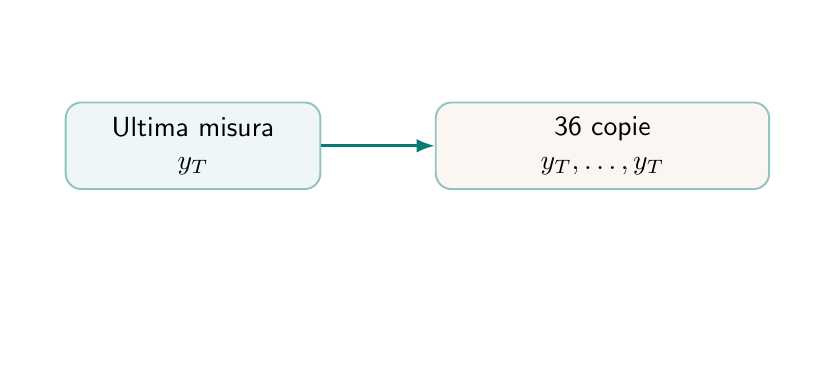
\begin{tikzpicture}[x=1cm,y=1cm]
\path[use as bounding box](-.1,-.15) rectangle(9.7,4.1);
\node[pFlow,text width=3cm,fill=GeoA!7] (a) at(2.0,2.6){Ultima misura\\$y_T$};
\node[pFlow,text width=4cm,fill=GeoB!7] (b) at(7.2,2.6){36 copie\\$y_T,\ldots,y_T$};
\draw[pEdge] (a) -- (b);
\end{tikzpicture}

\end{minipage}\end{lrbox}
\typeout{FULLBOX:013:PilotLeftBox:\the\ht\PilotLeftBox:\the\dp\PilotLeftBox}

\begin{lrbox}{\PilotRightBox}
\begin{minipage}[t]{7.55cm}\raggedright\color{Ink}\fontsize{11.3}{14.8}\selectfont
\PBody{La previsione resta orizzontale. È il centro naturale di un random walk senza deriva, con innovazioni future a media nulla.}
\vspace{2.5mm}
\PInfo{La previsione puntuale costante non implica incertezza costante: in un random walk la varianza dell’errore cresce con l’orizzonte.}
\PCode{R · ultimo valore}{013_esempio.R}
\end{minipage}\end{lrbox}
\typeout{FULLBOX:013:PilotRightBox:\the\ht\PilotRightBox:\the\dp\PilotRightBox}

\begin{tikzpicture}[remember picture,overlay]
\PilotChrome{L’ultimo valore prolunga il livello più recente}{II · RIFERIMENTI}{13}{Il riferimento all’ultimo valore conserva il livello, ma non aggiunge una stagione o una deriva.}
\node[anchor=north west,inner sep=0] at([xshift=.96cm,yshift=-2.13cm]current page.north west){\usebox{\PilotLeftBox}};
\node[anchor=north west,inner sep=0] at([xshift=11.52cm,yshift=-2.13cm]current page.north west){\usebox{\PilotRightBox}};
\node[anchor=north east,inner sep=0] at([xshift=17.65cm,yshift=-12.06cm]current page.north west){\color{Classical}\fontsize{7.7}{9.2}\selectfont\href{../../03_Notebook_svolti/M10_Futura/M10_N02.html}{M10\_N02 · notebook svolto}};
\end{tikzpicture}\end{frame}

\begin{frame}[plain]\hypertarget{slide14}{}
\bookmark[level=1,page=14]{Il riferimento stagionale ripete un ciclo già noto}
\begin{lrbox}{\TitleBox}
\begin{minipage}[t]{17.7cm}\raggedright\color{Ink}\fontsize{11.3}{14.8}\selectfont
\color{Navy}\bfseries\fontsize{20.6}{24.5}\selectfont Il riferimento stagionale ripete un ciclo già noto
\end{minipage}\end{lrbox}
\typeout{FULLBOX:014:TitleBox:\the\ht\TitleBox:\the\dp\TitleBox}

\begin{lrbox}{\RecallBox}
\begin{minipage}[t]{14.3cm}\raggedright\color{Ink}\fontsize{11.3}{14.8}\selectfont
\fontsize{10.3}{13.8}\selectfont A origine fissa il riferimento stagionale non può incorporare osservazioni future.
\end{minipage}\end{lrbox}
\typeout{FULLBOX:014:RecallBox:\the\ht\RecallBox:\the\dp\RecallBox}

\begin{lrbox}{\PilotLeftBox}
\begin{minipage}[t]{10.05cm}\raggedright\color{Ink}\fontsize{11.3}{14.8}\selectfont
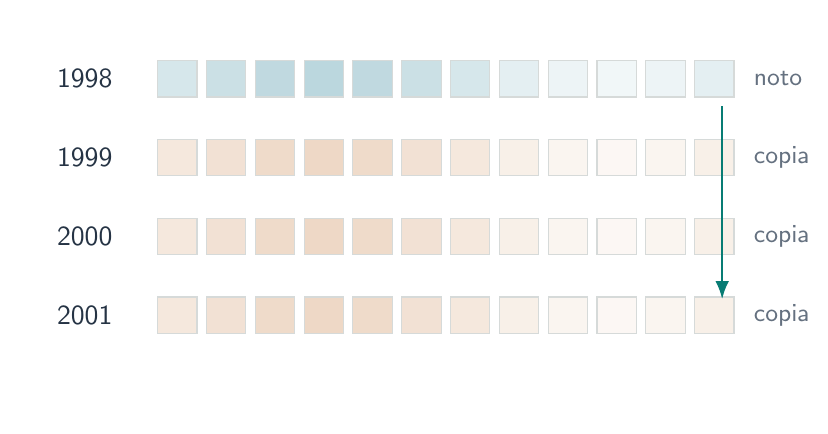
\begin{tikzpicture}[x=1cm,y=1cm]
\path[use as bounding box](-.1,-.15) rectangle(9.7,4.65);
\node[pLabel,anchor=east]at(1.1,4.0){1998};
\filldraw[fill=GeoA!18,draw=Rule](1.55,3.77)rectangle(2.05,4.23);
\filldraw[fill=GeoA!23,draw=Rule](2.17,3.77)rectangle(2.67,4.23);
\filldraw[fill=GeoA!28,draw=Rule](2.79,3.77)rectangle(3.29,4.23);
\filldraw[fill=GeoA!30,draw=Rule](3.41,3.77)rectangle(3.91,4.23);
\filldraw[fill=GeoA!28,draw=Rule](4.03,3.77)rectangle(4.53,4.23);
\filldraw[fill=GeoA!23,draw=Rule](4.65,3.77)rectangle(5.15,4.23);
\filldraw[fill=GeoA!18,draw=Rule](5.27,3.77)rectangle(5.77,4.23);
\filldraw[fill=GeoA!12,draw=Rule](5.89,3.77)rectangle(6.39,4.23);
\filldraw[fill=GeoA!8,draw=Rule](6.51,3.77)rectangle(7.01,4.23);
\filldraw[fill=GeoA!6,draw=Rule](7.13,3.77)rectangle(7.63,4.23);
\filldraw[fill=GeoA!8,draw=Rule](7.75,3.77)rectangle(8.25,4.23);
\filldraw[fill=GeoA!12,draw=Rule](8.370000000000001,3.77)rectangle(8.870000000000001,4.23);
\node[pNote,anchor=west]at(9.0,4.0){noto};
\node[pLabel,anchor=east]at(1.1,3.0){1999};
\filldraw[fill=GeoB!18,draw=Rule](1.55,2.77)rectangle(2.05,3.23);
\filldraw[fill=GeoB!23,draw=Rule](2.17,2.77)rectangle(2.67,3.23);
\filldraw[fill=GeoB!28,draw=Rule](2.79,2.77)rectangle(3.29,3.23);
\filldraw[fill=GeoB!30,draw=Rule](3.41,2.77)rectangle(3.91,3.23);
\filldraw[fill=GeoB!28,draw=Rule](4.03,2.77)rectangle(4.53,3.23);
\filldraw[fill=GeoB!23,draw=Rule](4.65,2.77)rectangle(5.15,3.23);
\filldraw[fill=GeoB!18,draw=Rule](5.27,2.77)rectangle(5.77,3.23);
\filldraw[fill=GeoB!12,draw=Rule](5.89,2.77)rectangle(6.39,3.23);
\filldraw[fill=GeoB!8,draw=Rule](6.51,2.77)rectangle(7.01,3.23);
\filldraw[fill=GeoB!6,draw=Rule](7.13,2.77)rectangle(7.63,3.23);
\filldraw[fill=GeoB!8,draw=Rule](7.75,2.77)rectangle(8.25,3.23);
\filldraw[fill=GeoB!12,draw=Rule](8.370000000000001,2.77)rectangle(8.870000000000001,3.23);
\node[pNote,anchor=west]at(9.0,3.0){copia};
\node[pLabel,anchor=east]at(1.1,2.0){2000};
\filldraw[fill=GeoB!18,draw=Rule](1.55,1.77)rectangle(2.05,2.23);
\filldraw[fill=GeoB!23,draw=Rule](2.17,1.77)rectangle(2.67,2.23);
\filldraw[fill=GeoB!28,draw=Rule](2.79,1.77)rectangle(3.29,2.23);
\filldraw[fill=GeoB!30,draw=Rule](3.41,1.77)rectangle(3.91,2.23);
\filldraw[fill=GeoB!28,draw=Rule](4.03,1.77)rectangle(4.53,2.23);
\filldraw[fill=GeoB!23,draw=Rule](4.65,1.77)rectangle(5.15,2.23);
\filldraw[fill=GeoB!18,draw=Rule](5.27,1.77)rectangle(5.77,2.23);
\filldraw[fill=GeoB!12,draw=Rule](5.89,1.77)rectangle(6.39,2.23);
\filldraw[fill=GeoB!8,draw=Rule](6.51,1.77)rectangle(7.01,2.23);
\filldraw[fill=GeoB!6,draw=Rule](7.13,1.77)rectangle(7.63,2.23);
\filldraw[fill=GeoB!8,draw=Rule](7.75,1.77)rectangle(8.25,2.23);
\filldraw[fill=GeoB!12,draw=Rule](8.370000000000001,1.77)rectangle(8.870000000000001,2.23);
\node[pNote,anchor=west]at(9.0,2.0){copia};
\node[pLabel,anchor=east]at(1.1,1.0){2001};
\filldraw[fill=GeoB!18,draw=Rule](1.55,0.77)rectangle(2.05,1.23);
\filldraw[fill=GeoB!23,draw=Rule](2.17,0.77)rectangle(2.67,1.23);
\filldraw[fill=GeoB!28,draw=Rule](2.79,0.77)rectangle(3.29,1.23);
\filldraw[fill=GeoB!30,draw=Rule](3.41,0.77)rectangle(3.91,1.23);
\filldraw[fill=GeoB!28,draw=Rule](4.03,0.77)rectangle(4.53,1.23);
\filldraw[fill=GeoB!23,draw=Rule](4.65,0.77)rectangle(5.15,1.23);
\filldraw[fill=GeoB!18,draw=Rule](5.27,0.77)rectangle(5.77,1.23);
\filldraw[fill=GeoB!12,draw=Rule](5.89,0.77)rectangle(6.39,1.23);
\filldraw[fill=GeoB!8,draw=Rule](6.51,0.77)rectangle(7.01,1.23);
\filldraw[fill=GeoB!6,draw=Rule](7.13,0.77)rectangle(7.63,1.23);
\filldraw[fill=GeoB!8,draw=Rule](7.75,0.77)rectangle(8.25,1.23);
\filldraw[fill=GeoB!12,draw=Rule](8.370000000000001,0.77)rectangle(8.870000000000001,1.23);
\node[pNote,anchor=west]at(9.0,1.0){copia};
\draw[pEdge](8.72,3.65)--(8.72,1.2);
\end{tikzpicture}
\[\widehat y_{T+h\mid T}=y_{T+h-12\lceil h/12\rceil}\]

\end{minipage}\end{lrbox}
\typeout{FULLBOX:014:PilotLeftBox:\the\ht\PilotLeftBox:\the\dp\PilotLeftBox}

\begin{lrbox}{\PilotRightBox}
\begin{minipage}[t]{7.55cm}\raggedright\color{Ink}\fontsize{11.3}{14.8}\selectfont
\PBody{Per i primi 12 mesi si riusa l’ultimo anno osservato. A origine fissa, lo stesso ciclo si ripete anche nel secondo e nel terzo anno di previsione.}
\vspace{2.5mm}
\PInfo{Gennaio 2000 usa gennaio 1998, perché gennaio 1999 non era disponibile a dicembre 1998.}
\PCode{R · ripetere l’ultima stagione}{014_esempio.R}
\end{minipage}\end{lrbox}
\typeout{FULLBOX:014:PilotRightBox:\the\ht\PilotRightBox:\the\dp\PilotRightBox}

\begin{tikzpicture}[remember picture,overlay]
\PilotChrome{Il riferimento stagionale ripete un ciclo già noto}{II · RIFERIMENTI}{14}{A origine fissa il riferimento stagionale non può incorporare osservazioni future.}
\node[anchor=north west,inner sep=0] at([xshift=.96cm,yshift=-2.13cm]current page.north west){\usebox{\PilotLeftBox}};
\node[anchor=north west,inner sep=0] at([xshift=11.52cm,yshift=-2.13cm]current page.north west){\usebox{\PilotRightBox}};
\node[anchor=north east,inner sep=0] at([xshift=17.65cm,yshift=-12.06cm]current page.north west){\color{Classical}\fontsize{7.7}{9.2}\selectfont\href{../../03_Notebook_svolti/M10_Futura/M10_N20.html}{M10\_N20 · notebook svolto}};
\end{tikzpicture}\end{frame}

\begin{frame}[plain]\hypertarget{slide15}{}
\bookmark[level=1,page=15]{L’indice stagionale va verificato sui mesi}
\begin{lrbox}{\TitleBox}
\begin{minipage}[t]{17.7cm}\raggedright\color{Ink}\fontsize{11.3}{14.8}\selectfont
\color{Navy}\bfseries\fontsize{20.6}{24.5}\selectfont L’indice stagionale va verificato sui mesi
\end{minipage}\end{lrbox}
\typeout{FULLBOX:015:TitleBox:\the\ht\TitleBox:\the\dp\TitleBox}

\begin{lrbox}{\RecallBox}
\begin{minipage}[t]{14.3cm}\raggedright\color{Ink}\fontsize{11.3}{14.8}\selectfont
\fontsize{10.3}{13.8}\selectfont L’allineamento temporale è parte della correttezza della previsione.
\end{minipage}\end{lrbox}
\typeout{FULLBOX:015:RecallBox:\the\ht\RecallBox:\the\dp\RecallBox}

\begin{lrbox}{\PilotLeftBox}
\begin{minipage}[t]{10.05cm}\raggedright\color{Ink}\fontsize{11.3}{14.8}\selectfont
{\fontsize{10.2}{13.1}\selectfont\renewcommand{\arraystretch}{1.45}\begin{tabular}{@{}p{4.1cm}p{5.0cm}@{}}\toprule
\textbf{Previsione} & \textbf{Valore storico utilizzato}\\\midrule
Gennaio 1999 & Gennaio 1998\\
Dicembre 1999 & Dicembre 1998\\
Gennaio 2000 & Gennaio 1998\\
Dicembre 2001 & Dicembre 1998\\
\bottomrule\end{tabular}}

\end{minipage}\end{lrbox}
\typeout{FULLBOX:015:PilotLeftBox:\the\ht\PilotLeftBox:\the\dp\PilotLeftBox}

\begin{lrbox}{\PilotRightBox}
\begin{minipage}[t]{7.55cm}\raggedright\color{Ink}\fontsize{11.3}{14.8}\selectfont
\PBody{Una sequenza lunga il numero corretto di righe può avere una fase sbagliata. Il calendario permette di riconoscere una rotazione accidentale del ciclo.}
\vspace{2.5mm}
\PInfo{I test del notebook confrontano la corrispondenza tra mese previsto e mese riutilizzato, oltre alla lunghezza del vettore.}
\PCode{R · controllare la fase}{015_esempio.R}
\end{minipage}\end{lrbox}
\typeout{FULLBOX:015:PilotRightBox:\the\ht\PilotRightBox:\the\dp\PilotRightBox}

\begin{tikzpicture}[remember picture,overlay]
\PilotChrome{L’indice stagionale va verificato sui mesi}{II · RIFERIMENTI}{15}{L’allineamento temporale è parte della correttezza della previsione.}
\node[anchor=north west,inner sep=0] at([xshift=.96cm,yshift=-2.13cm]current page.north west){\usebox{\PilotLeftBox}};
\node[anchor=north west,inner sep=0] at([xshift=11.52cm,yshift=-2.13cm]current page.north west){\usebox{\PilotRightBox}};
\node[anchor=north east,inner sep=0] at([xshift=17.65cm,yshift=-12.06cm]current page.north west){\color{Classical}\fontsize{7.7}{9.2}\selectfont\href{../../03_Notebook_svolti/M10_Futura/M10_N20.html}{M10\_N20 · notebook svolto}};
\end{tikzpicture}\end{frame}

\begin{frame}[plain]\hypertarget{slide16}{}
\bookmark[level=1,page=16]{La deriva prolunga una variazione media}
\begin{lrbox}{\TitleBox}
\begin{minipage}[t]{17.7cm}\raggedright\color{Ink}\fontsize{11.3}{14.8}\selectfont
\color{Navy}\bfseries\fontsize{20.6}{24.5}\selectfont La deriva prolunga una variazione media
\end{minipage}\end{lrbox}
\typeout{FULLBOX:016:TitleBox:\the\ht\TitleBox:\the\dp\TitleBox}

\begin{lrbox}{\RecallBox}
\begin{minipage}[t]{14.3cm}\raggedright\color{Ink}\fontsize{11.3}{14.8}\selectfont
\fontsize{10.3}{13.8}\selectfont Una deriva semplice può essere competitiva, ma la sua pendenza dipende dagli estremi osservati.
\end{minipage}\end{lrbox}
\typeout{FULLBOX:016:RecallBox:\the\ht\RecallBox:\the\dp\RecallBox}

\begin{lrbox}{\PilotLeftBox}
\begin{minipage}[t]{10.05cm}\raggedright\color{Ink}\fontsize{11.3}{14.8}\selectfont
\[\widehat\delta=\frac{y_T-y_1}{T-1}\]
\[\widehat y_{T+h\mid T}^{\,\mathrm{deriva}}=y_T+h\widehat\delta\]
\PInfo{La pendenza è una variazione per mese. Non è la pendenza di una regressione stimata su tutti i punti.}

\end{minipage}\end{lrbox}
\typeout{FULLBOX:016:PilotLeftBox:\the\ht\PilotLeftBox:\the\dp\PilotLeftBox}

\begin{lrbox}{\PilotRightBox}
\begin{minipage}[t]{7.55cm}\raggedright\color{Ink}\fontsize{11.3}{14.8}\selectfont
\PBody{Il metodo unisce il primo e l’ultimo livello e prolunga quella pendenza. Gli estremi possono influenzarlo molto, specialmente in presenza di stagione o anomalie.}
\vspace{2.5mm}
\PBody{La deriva è un riferimento esplicito per la crescita: evita che il modello stagionale venga confrontato soltanto con metodi privi di tendenza.}
\vspace{2.5mm}
\PCode{R · stimare la deriva}{016_esempio.R}
\end{minipage}\end{lrbox}
\typeout{FULLBOX:016:PilotRightBox:\the\ht\PilotRightBox:\the\dp\PilotRightBox}

\begin{tikzpicture}[remember picture,overlay]
\PilotChrome{La deriva prolunga una variazione media}{II · RIFERIMENTI}{16}{Una deriva semplice può essere competitiva, ma la sua pendenza dipende dagli estremi osservati.}
\node[anchor=north west,inner sep=0] at([xshift=.96cm,yshift=-2.13cm]current page.north west){\usebox{\PilotLeftBox}};
\node[anchor=north west,inner sep=0] at([xshift=11.52cm,yshift=-2.13cm]current page.north west){\usebox{\PilotRightBox}};
\node[anchor=north east,inner sep=0] at([xshift=17.65cm,yshift=-12.06cm]current page.north west){\color{Classical}\fontsize{7.7}{9.2}\selectfont\href{../../03_Notebook_svolti/M10_Futura/M10_N02.html}{M10\_N02 · notebook svolto}};
\end{tikzpicture}\end{frame}

\begin{frame}[plain]\hypertarget{slide17}{}
\bookmark[level=1,page=17]{Ogni riferimento porta ipotesi riconoscibili}
\begin{lrbox}{\TitleBox}
\begin{minipage}[t]{17.7cm}\raggedright\color{Ink}\fontsize{11.3}{14.8}\selectfont
\color{Navy}\bfseries\fontsize{20.6}{24.5}\selectfont Ogni riferimento porta ipotesi riconoscibili
\end{minipage}\end{lrbox}
\typeout{FULLBOX:017:TitleBox:\the\ht\TitleBox:\the\dp\TitleBox}

\begin{lrbox}{\RecallBox}
\begin{minipage}[t]{14.3cm}\raggedright\color{Ink}\fontsize{11.3}{14.8}\selectfont
\fontsize{10.3}{13.8}\selectfont Un riferimento va giudicato per la struttura che conserva e per quella che trascura.
\end{minipage}\end{lrbox}
\typeout{FULLBOX:017:RecallBox:\the\ht\RecallBox:\the\dp\RecallBox}

\begin{lrbox}{\PilotLeftBox}
\begin{minipage}[t]{10.05cm}\raggedright\color{Ink}\fontsize{11.3}{14.8}\selectfont
{\fontsize{10.2}{13.1}\selectfont\renewcommand{\arraystretch}{1.45}\begin{tabular}{@{}p{2.9cm}p{6.1cm}@{}}\toprule
\textbf{Metodo} & \textbf{Rischio da discutere}\\\midrule
Media & Livello storico lontano da quello attuale\\
Ultimo & Mancata crescita e mancata stagione\\
Stagionale & Ciclo stabile senza crescita fra anni\\
Deriva & Pendenza costante e stagione assente\\
\bottomrule\end{tabular}}

\end{minipage}\end{lrbox}
\typeout{FULLBOX:017:PilotLeftBox:\the\ht\PilotLeftBox:\the\dp\PilotLeftBox}

\begin{lrbox}{\PilotRightBox}
\begin{minipage}[t]{7.55cm}\raggedright\color{Ink}\fontsize{11.3}{14.8}\selectfont
\PBody{I riferimenti rappresentano ipotesi diverse. Osservare come sbagliano aiuta a capire quale informazione aggiunge il modello.}
\vspace{2.5mm}
\PInfo{Una previsione stagionale che ripete il 1998 può riconoscere i mesi alti e bassi e sottostimare il livello degli anni successivi.}
\PBody{Le ipotesi si discutono prima della graduatoria. La prestazione si misura poi sugli stessi valori futuri.}
\vspace{2.5mm}

\end{minipage}\end{lrbox}
\typeout{FULLBOX:017:PilotRightBox:\the\ht\PilotRightBox:\the\dp\PilotRightBox}

\begin{tikzpicture}[remember picture,overlay]
\PilotChrome{Ogni riferimento porta ipotesi riconoscibili}{II · RIFERIMENTI}{17}{Un riferimento va giudicato per la struttura che conserva e per quella che trascura.}
\node[anchor=north west,inner sep=0] at([xshift=.96cm,yshift=-2.13cm]current page.north west){\usebox{\PilotLeftBox}};
\node[anchor=north west,inner sep=0] at([xshift=11.52cm,yshift=-2.13cm]current page.north west){\usebox{\PilotRightBox}};
\end{tikzpicture}\end{frame}

\begin{frame}[plain]\hypertarget{slide18}{}
\bookmark[level=1,page=18]{Le traiettorie rendono visibili le differenze}
\begin{lrbox}{\TitleBox}
\begin{minipage}[t]{17.7cm}\raggedright\color{Ink}\fontsize{11.3}{14.8}\selectfont
\color{Navy}\bfseries\fontsize{20.6}{24.5}\selectfont Le traiettorie rendono visibili le differenze
\end{minipage}\end{lrbox}
\typeout{FULLBOX:018:TitleBox:\the\ht\TitleBox:\the\dp\TitleBox}

\begin{lrbox}{\RecallBox}
\begin{minipage}[t]{14.3cm}\raggedright\color{Ink}\fontsize{11.3}{14.8}\selectfont
\fontsize{10.3}{13.8}\selectfont Disegnare le previsioni permette di controllare subito livello, stagione e orientamento della tendenza.
\end{minipage}\end{lrbox}
\typeout{FULLBOX:018:RecallBox:\the\ht\RecallBox:\the\dp\RecallBox}

\begin{lrbox}{\PilotLeftBox}
\begin{minipage}[t]{10.05cm}\raggedright\color{Ink}\fontsize{11.3}{14.8}\selectfont
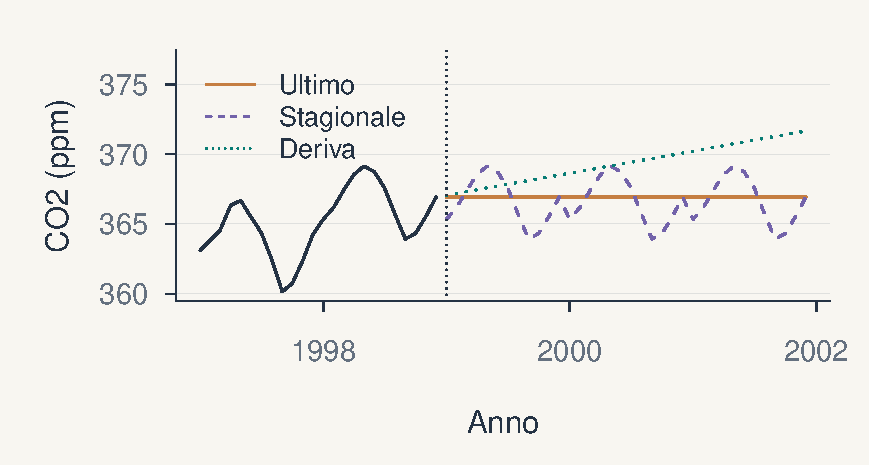
\includegraphics[width=9.85cm,height=5.25cm,keepaspectratio]{Risultati/Figure/02_baseline_CO2.pdf}
\vspace{1.5mm}
\PSmall{Previsioni emesse alla stessa origine. Il grafico mostra le ipotesi dei riferimenti prima delle metriche.}

\end{minipage}\end{lrbox}
\typeout{FULLBOX:018:PilotLeftBox:\the\ht\PilotLeftBox:\the\dp\PilotLeftBox}

\begin{lrbox}{\PilotRightBox}
\begin{minipage}[t]{7.55cm}\raggedright\color{Ink}\fontsize{11.3}{14.8}\selectfont
\PBody{L’ultimo valore produce una linea orizzontale. La deriva cresce in modo lineare. Il riferimento stagionale ripete la stessa forma annuale.}
\vspace{2.5mm}
\PInfo{La differenza tra metodi riguarda l’informazione mantenuta dal passato. Il test finale quantificherà quanto queste scelte siano utili.}
\PSmall{Per confronti numerici usare le tabelle eseguite, non misure ricavate a occhio dal grafico.}

\end{minipage}\end{lrbox}
\typeout{FULLBOX:018:PilotRightBox:\the\ht\PilotRightBox:\the\dp\PilotRightBox}

\begin{tikzpicture}[remember picture,overlay]
\PilotChrome{Le traiettorie rendono visibili le differenze}{II · RIFERIMENTI}{18}{Disegnare le previsioni permette di controllare subito livello, stagione e orientamento della tendenza.}
\node[anchor=north west,inner sep=0] at([xshift=.96cm,yshift=-2.13cm]current page.north west){\usebox{\PilotLeftBox}};
\node[anchor=north west,inner sep=0] at([xshift=11.52cm,yshift=-2.13cm]current page.north west){\usebox{\PilotRightBox}};
\node[anchor=north east,inner sep=0] at([xshift=17.65cm,yshift=-12.06cm]current page.north west){\color{Classical}\fontsize{7.7}{9.2}\selectfont\href{../../03_Notebook_svolti/M10_Futura/M10_N02.html}{M10\_N02 · notebook svolto}};
\end{tikzpicture}\end{frame}

\begin{frame}[plain]\hypertarget{slide19}{}
\bookmark[level=1,page=19]{Un buon adattamento non basta a prevedere bene}
\begin{lrbox}{\TitleBox}
\begin{minipage}[t]{17.7cm}\raggedright\color{Ink}\fontsize{11.3}{14.8}\selectfont
\color{Navy}\bfseries\fontsize{20.6}{24.5}\selectfont Un buon adattamento non basta a prevedere bene
\end{minipage}\end{lrbox}
\typeout{FULLBOX:019:TitleBox:\the\ht\TitleBox:\the\dp\TitleBox}

\begin{lrbox}{\RecallBox}
\begin{minipage}[t]{14.3cm}\raggedright\color{Ink}\fontsize{11.3}{14.8}\selectfont
\fontsize{10.3}{13.8}\selectfont La capacità di spiegare il passato deve essere accompagnata da una prova sul futuro disponibile in seguito.
\end{minipage}\end{lrbox}
\typeout{FULLBOX:019:RecallBox:\the\ht\RecallBox:\the\dp\RecallBox}

\begin{lrbox}{\PilotLeftBox}
\begin{minipage}[t]{10.05cm}\raggedright\color{Ink}\fontsize{11.3}{14.8}\selectfont
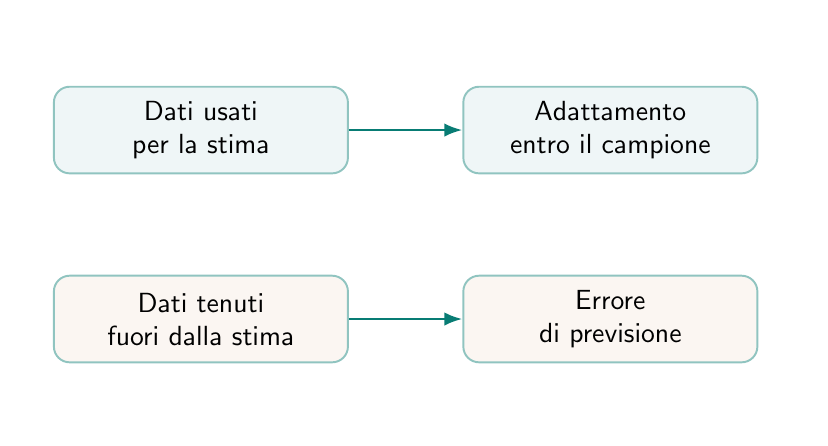
\begin{tikzpicture}[x=1cm,y=1cm]
\path[use as bounding box](-.1,-.15) rectangle(9.7,4.8);
\node[pFlow,text width=3.5cm,fill=GeoA!7] (a) at(2.1,3.5){Dati usati\\per la stima};
\node[pFlow,text width=3.5cm,fill=GeoA!7] (b) at(7.3,3.5){Adattamento\\entro il campione};
\node[pFlow,text width=3.5cm,fill=GeoB!7] (c) at(2.1,1.1){Dati tenuti\\fuori dalla stima};
\node[pFlow,text width=3.5cm,fill=GeoB!7] (d) at(7.3,1.1){Errore\\di previsione};
\draw[pEdge] (a) -- (b);
\draw[pEdge] (c) -- (d);
\end{tikzpicture}

\end{minipage}\end{lrbox}
\typeout{FULLBOX:019:PilotLeftBox:\the\ht\PilotLeftBox:\the\dp\PilotLeftBox}

\begin{lrbox}{\PilotRightBox}
\begin{minipage}[t]{7.55cm}\raggedright\color{Ink}\fontsize{11.3}{14.8}\selectfont
\PBody{Aggiungere parametri può ridurre l’errore sul campione usato per stimarli. Questa riduzione non garantisce un miglioramento sui valori successivi.}
\vspace{2.5mm}
\PInfo{Il residuo del modello e l’errore di previsione fuori campione hanno ruoli distinti. La diagnostica dei residui non sostituisce la validazione.}
\PBody{La verifica deve ricostruire il momento in cui la previsione sarebbe stata emessa.}
\vspace{2.5mm}

\end{minipage}\end{lrbox}
\typeout{FULLBOX:019:PilotRightBox:\the\ht\PilotRightBox:\the\dp\PilotRightBox}

\begin{tikzpicture}[remember picture,overlay]
\PilotChrome{Un buon adattamento non basta a prevedere bene}{II · RIFERIMENTI}{19}{La capacità di spiegare il passato deve essere accompagnata da una prova sul futuro disponibile in seguito.}
\node[anchor=north west,inner sep=0] at([xshift=.96cm,yshift=-2.13cm]current page.north west){\usebox{\PilotLeftBox}};
\node[anchor=north west,inner sep=0] at([xshift=11.52cm,yshift=-2.13cm]current page.north west){\usebox{\PilotRightBox}};
\end{tikzpicture}\end{frame}

\begin{frame}[plain]\hypertarget{slide20}{}
\bookmark[level=1,page=20]{Due origini diverse definiscono due esperimenti}
\begin{lrbox}{\TitleBox}
\begin{minipage}[t]{17.7cm}\raggedright\color{Ink}\fontsize{11.3}{14.8}\selectfont
\color{Navy}\bfseries\fontsize{20.6}{24.5}\selectfont Due origini diverse definiscono due esperimenti
\end{minipage}\end{lrbox}
\typeout{FULLBOX:020:TitleBox:\the\ht\TitleBox:\the\dp\TitleBox}

\begin{lrbox}{\RecallBox}
\begin{minipage}[t]{14.3cm}\raggedright\color{Ink}\fontsize{11.3}{14.8}\selectfont
\fontsize{10.3}{13.8}\selectfont L’origine della previsione deve restare associata a ogni errore misurato.
\end{minipage}\end{lrbox}
\typeout{FULLBOX:020:RecallBox:\the\ht\RecallBox:\the\dp\RecallBox}

\begin{lrbox}{\PilotLeftBox}
\begin{minipage}[t]{10.05cm}\raggedright\color{Ink}\fontsize{11.3}{14.8}\selectfont
{\fontsize{10.2}{13.1}\selectfont\renewcommand{\arraystretch}{1.45}\begin{tabular}{@{}p{4.5cm}p{4.5cm}@{}}\toprule
\textbf{Origine fissa} & \textbf{Origini aggiornate}\\\midrule
Una stima a dicembre 1998 & Nuove stime quando arrivano dati\\
36 orizzonti dalla stessa origine & Più previsioni emesse nel tempo\\
Il ciclo 1998 viene ripetuto & Il ciclo può incorporare nuovi mesi\\
Una traiettoria storica riservata & Più coppie origine--orizzonte\\
\bottomrule\end{tabular}}

\end{minipage}\end{lrbox}
\typeout{FULLBOX:020:PilotLeftBox:\the\ht\PilotLeftBox:\the\dp\PilotLeftBox}

\begin{lrbox}{\PilotRightBox}
\begin{minipage}[t]{7.55cm}\raggedright\color{Ink}\fontsize{11.3}{14.8}\selectfont
\PBody{Aggiornare il modello ogni mese è possibile, ma cambia il compito. Non si può attribuire alla previsione emessa nel 1998 l’informazione arrivata nel 1999.}
\vspace{2.5mm}
\PInfo{Il laboratorio centrale conserva un’origine fissa per il test finale. La validazione interna usa origini successive, tutte precedenti al test.}

\end{minipage}\end{lrbox}
\typeout{FULLBOX:020:PilotRightBox:\the\ht\PilotRightBox:\the\dp\PilotRightBox}

\begin{tikzpicture}[remember picture,overlay]
\PilotChrome{Due origini diverse definiscono due esperimenti}{II · RIFERIMENTI}{20}{L’origine della previsione deve restare associata a ogni errore misurato.}
\node[anchor=north west,inner sep=0] at([xshift=.96cm,yshift=-2.13cm]current page.north west){\usebox{\PilotLeftBox}};
\node[anchor=north west,inner sep=0] at([xshift=11.52cm,yshift=-2.13cm]current page.north west){\usebox{\PilotRightBox}};
\end{tikzpicture}\end{frame}

\begin{frame}[plain]\hypertarget{slide21}{}
\bookmark[level=1,page=21]{Le origini interne fanno una prova prima del test}
\begin{lrbox}{\TitleBox}
\begin{minipage}[t]{17.7cm}\raggedright\color{Ink}\fontsize{11.3}{14.8}\selectfont
\color{Navy}\bfseries\fontsize{20.6}{24.5}\selectfont Le origini interne fanno una prova prima del test
\end{minipage}\end{lrbox}
\typeout{FULLBOX:021:TitleBox:\the\ht\TitleBox:\the\dp\TitleBox}

\begin{lrbox}{\RecallBox}
\begin{minipage}[t]{14.3cm}\raggedright\color{Ink}\fontsize{11.3}{14.8}\selectfont
\fontsize{10.3}{13.8}\selectfont La validazione temporale ripete il compito previsionale senza aprire il test finale.
\end{minipage}\end{lrbox}
\typeout{FULLBOX:021:RecallBox:\the\ht\RecallBox:\the\dp\RecallBox}

\begin{lrbox}{\PilotLeftBox}
\begin{minipage}[t]{10.05cm}\raggedright\color{Ink}\fontsize{11.3}{14.8}\selectfont
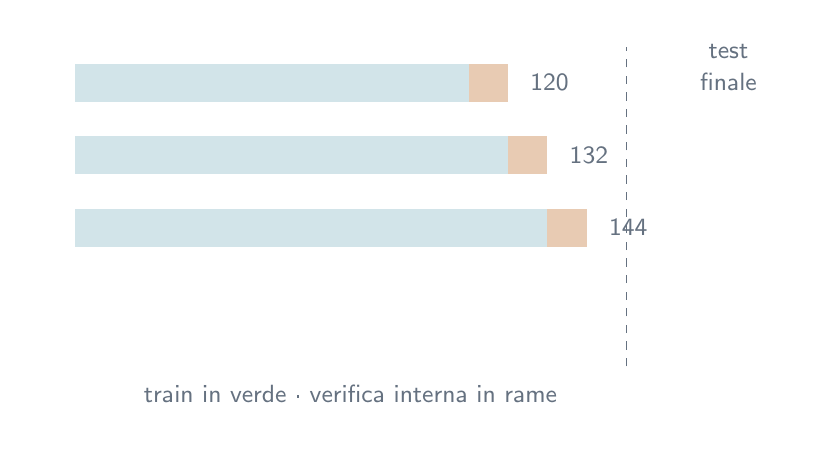
\begin{tikzpicture}[x=1cm,y=1cm]
\path[use as bounding box](-.1,-.15) rectangle(9.7,4.9);
\fill[GeoA!20](.5,3.96)rectangle(5.500,4.44);
\fill[GeoB!40](5.500,3.96)rectangle(6.000,4.44);
\node[pNote,anchor=west]at(6.160,4.2){120};
\fill[GeoA!20](.5,3.04)rectangle(6.000,3.5200000000000005);
\fill[GeoB!40](6.000,3.04)rectangle(6.500,3.5200000000000005);
\node[pNote,anchor=west]at(6.660,3.2800000000000002){132};
\fill[GeoA!20](.5,2.12)rectangle(6.500,2.6000000000000005);
\fill[GeoB!40](6.500,2.12)rectangle(7.000,2.6000000000000005);
\node[pNote,anchor=west]at(7.160,2.3600000000000003){144};
\draw[Muted,dashed](7.500,.6)--(7.500,4.65);
\node[pNote]at(4,.25){train in verde · verifica interna in rame};
\node[pNote]at(8.8,4.4){test\\finale};
\end{tikzpicture}
\[T_o\in\{120,132,144\},\qquad h=1,\ldots,12\]

\end{minipage}\end{lrbox}
\typeout{FULLBOX:021:PilotLeftBox:\the\ht\PilotLeftBox:\the\dp\PilotLeftBox}

\begin{lrbox}{\PilotRightBox}
\begin{minipage}[t]{7.55cm}\raggedright\color{Ink}\fontsize{11.3}{14.8}\selectfont
\PBody{A ciascuna origine si ricostruisce il passato disponibile e si stima di nuovo. I 12 mesi successivi diventano la verifica di quella previsione.}
\vspace{2.5mm}
\PInfo{Le tre finestre di verifica coprono 1995, 1996 e 1997. Il 1998 rimane disponibile per la stima finale sui 168 mesi.}
\PSmall{Approfondiremo finestre, metriche e dipendenza fra errori nella sezione sulla validazione.}

\end{minipage}\end{lrbox}
\typeout{FULLBOX:021:PilotRightBox:\the\ht\PilotRightBox:\the\dp\PilotRightBox}

\begin{tikzpicture}[remember picture,overlay]
\PilotChrome{Le origini interne fanno una prova prima del test}{II · RIFERIMENTI}{21}{La validazione temporale ripete il compito previsionale senza aprire il test finale.}
\node[anchor=north west,inner sep=0] at([xshift=.96cm,yshift=-2.13cm]current page.north west){\usebox{\PilotLeftBox}};
\node[anchor=north west,inner sep=0] at([xshift=11.52cm,yshift=-2.13cm]current page.north west){\usebox{\PilotRightBox}};
\node[anchor=north east,inner sep=0] at([xshift=17.65cm,yshift=-12.06cm]current page.north west){\color{Classical}\fontsize{7.7}{9.2}\selectfont\href{../../03_Notebook_svolti/M10_Futura/M10_N05.html}{M10\_N05 · notebook svolto}};
\end{tikzpicture}\end{frame}

\begin{frame}[plain]\hypertarget{slide22}{}
\bookmark[level=1,page=22]{Laboratorio: quattro riferimenti confrontabili}
\begin{lrbox}{\TitleBox}
\begin{minipage}[t]{17.7cm}\raggedright\color{Ink}\fontsize{11.3}{14.8}\selectfont
\color{Navy}\bfseries\fontsize{20.6}{24.5}\selectfont Laboratorio: quattro riferimenti confrontabili
\end{minipage}\end{lrbox}
\typeout{FULLBOX:022:TitleBox:\the\ht\TitleBox:\the\dp\TitleBox}

\begin{lrbox}{\RecallBox}
\begin{minipage}[t]{14.3cm}\raggedright\color{Ink}\fontsize{11.3}{14.8}\selectfont
\fontsize{10.3}{13.8}\selectfont La comparabilità è una condizione del confronto, non un dettaglio da controllare dopo.
\end{minipage}\end{lrbox}
\typeout{FULLBOX:022:RecallBox:\the\ht\RecallBox:\the\dp\RecallBox}

\begin{lrbox}{\PilotLeftBox}
\begin{minipage}[t]{10.05cm}\raggedright\color{Ink}\fontsize{11.3}{14.8}\selectfont
\PLabel{Controlli richiesti}
{\fontsize{10.2}{13.1}\selectfont\renewcommand{\arraystretch}{1.45}\begin{tabular}{@{}p{2.6cm}p{6.4cm}@{}}\toprule
\textbf{Controllo} & \textbf{Criterio}\\\midrule
Origine & Identica per ogni metodo\\
Date & 36 mesi nello stesso ordine\\
Scala & ppm per osservazioni e previsioni\\
Stagione & Ultimi 12 mesi ripetuti\\
Futuro & Nessuna lettura del test nella stima\\
\bottomrule\end{tabular}}

\end{minipage}\end{lrbox}
\typeout{FULLBOX:022:PilotLeftBox:\the\ht\PilotLeftBox:\the\dp\PilotLeftBox}

\begin{lrbox}{\PilotRightBox}
\begin{minipage}[t]{7.55cm}\raggedright\color{Ink}\fontsize{11.3}{14.8}\selectfont
\PBody{M10\_N02 costruisce i riferimenti; M10\_N20 verifica la stagione. La funzione comune restituisce vettori confrontabili.}
\vspace{2.5mm}
\PInfo{Verificare la forma delle previsioni prima di calcolare gli errori. Un errore di allineamento può sembrare una cattiva prestazione del metodo.}
\PCode{R · contratto dei riferimenti}{022_esempio.R}
\end{minipage}\end{lrbox}
\typeout{FULLBOX:022:PilotRightBox:\the\ht\PilotRightBox:\the\dp\PilotRightBox}

\begin{tikzpicture}[remember picture,overlay]
\PilotChrome{Laboratorio: quattro riferimenti confrontabili}{II · RIFERIMENTI}{22}{La comparabilità è una condizione del confronto, non un dettaglio da controllare dopo.}
\node[anchor=north west,inner sep=0] at([xshift=.96cm,yshift=-2.13cm]current page.north west){\usebox{\PilotLeftBox}};
\node[anchor=north west,inner sep=0] at([xshift=11.52cm,yshift=-2.13cm]current page.north west){\usebox{\PilotRightBox}};
\node[anchor=north east,inner sep=0] at([xshift=17.65cm,yshift=-12.06cm]current page.north west){\color{Classical}\fontsize{7.7}{9.2}\selectfont\href{../../03_Notebook_svolti/M10_Futura/M10_N02.html}{M10\_N02 · notebook svolto}};
\end{tikzpicture}\end{frame}

\begin{frame}[plain]\hypertarget{slide23}{}
\bookmark[level=0,page=23]{III · MEMORIA E INNOVAZIONI}
\bookmark[level=1,page=23]{Un AR(1) separa memoria e innovazione}
\begin{lrbox}{\TitleBox}
\begin{minipage}[t]{17.7cm}\raggedright\color{Ink}\fontsize{11.3}{14.8}\selectfont
\color{Navy}\bfseries\fontsize{20.6}{24.5}\selectfont Un AR(1) separa memoria e innovazione
\end{minipage}\end{lrbox}
\typeout{FULLBOX:023:TitleBox:\the\ht\TitleBox:\the\dp\TitleBox}

\begin{lrbox}{\RecallBox}
\begin{minipage}[t]{14.3cm}\raggedright\color{Ink}\fontsize{11.3}{14.8}\selectfont
\fontsize{10.3}{13.8}\selectfont La memoria trasmette informazione passata; l’innovazione rappresenta la parte nuova.
\end{minipage}\end{lrbox}
\typeout{FULLBOX:023:RecallBox:\the\ht\RecallBox:\the\dp\RecallBox}

\begin{lrbox}{\PilotLeftBox}
\begin{minipage}[t]{10.05cm}\raggedright\color{Ink}\fontsize{11.3}{14.8}\selectfont
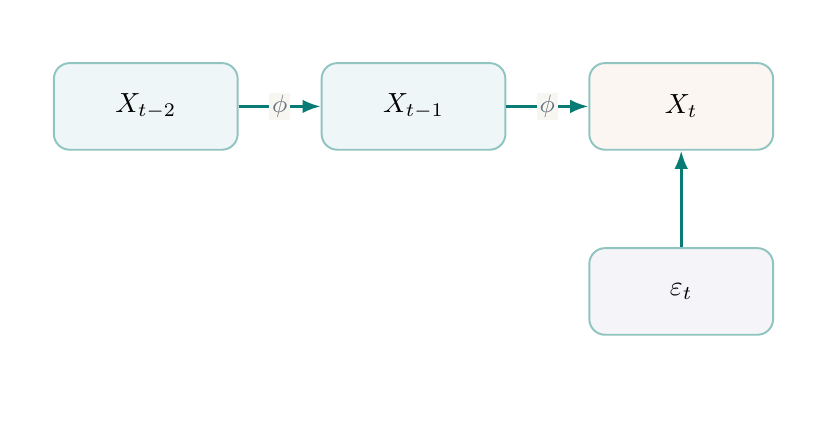
\begin{tikzpicture}[x=1cm,y=1cm]
\path[use as bounding box](-.1,-.15) rectangle(9.7,4.5);
\node[pFlow,text width=2.1cm,fill=GeoA!7] (a) at(1.4,3.5){$X_{t-2}$};
\node[pFlow,text width=2.1cm,fill=GeoA!7] (b) at(4.8,3.5){$X_{t-1}$};
\node[pFlow,text width=2.1cm,fill=GeoB!7] (c) at(8.2,3.5){$X_t$};
\node[pFlow,text width=2.1cm,fill=GeoC!7] (u) at(8.2,1.15){$\varepsilon_t$};
\draw[pEdge] (a) -- node[pNote,fill=Paper,inner sep=1pt]{$\phi$} (b);
\draw[pEdge] (b) -- node[pNote,fill=Paper,inner sep=1pt]{$\phi$} (c);
\draw[pEdge] (u) -- (c);
\end{tikzpicture}
\[X_t=\phi X_{t-1}+\varepsilon_t\]

\end{minipage}\end{lrbox}
\typeout{FULLBOX:023:PilotLeftBox:\the\ht\PilotLeftBox:\the\dp\PilotLeftBox}

\begin{lrbox}{\PilotRightBox}
\begin{minipage}[t]{7.55cm}\raggedright\color{Ink}\fontsize{11.3}{14.8}\selectfont
\PBody{Nel processo centrato, una parte del valore corrente dipende dal passato. L’innovazione aggiunge ciò che il modello non poteva prevedere al passo precedente.}
\vspace{2.5mm}
\PInfo{Assumiamo innovazioni a media nulla, varianza $\sigma^2$ e indipendenti dal passato. La normalità è un’ipotesi ulteriore, utile per intervalli gaussiani.}
\PSmall{Se $X_t$ è centrato rispetto a $\mu$, la serie originale è $Y_t=\mu+X_t$.}

\end{minipage}\end{lrbox}
\typeout{FULLBOX:023:PilotRightBox:\the\ht\PilotRightBox:\the\dp\PilotRightBox}

\begin{tikzpicture}[remember picture,overlay]
\PilotChrome{Un AR(1) separa memoria e innovazione}{III · MEMORIA E INNOVAZIONI}{23}{La memoria trasmette informazione passata; l’innovazione rappresenta la parte nuova.}
\node[anchor=north west,inner sep=0] at([xshift=.96cm,yshift=-2.13cm]current page.north west){\usebox{\PilotLeftBox}};
\node[anchor=north west,inner sep=0] at([xshift=11.52cm,yshift=-2.13cm]current page.north west){\usebox{\PilotRightBox}};
\end{tikzpicture}\end{frame}

\begin{frame}[plain]\hypertarget{slide24}{}
\bookmark[level=1,page=24]{Media e intercetta non sono lo stesso parametro}
\begin{lrbox}{\TitleBox}
\begin{minipage}[t]{17.7cm}\raggedright\color{Ink}\fontsize{11.3}{14.8}\selectfont
\color{Navy}\bfseries\fontsize{20.6}{24.5}\selectfont Media e intercetta non sono lo stesso parametro
\end{minipage}\end{lrbox}
\typeout{FULLBOX:024:TitleBox:\the\ht\TitleBox:\the\dp\TitleBox}

\begin{lrbox}{\RecallBox}
\begin{minipage}[t]{14.3cm}\raggedright\color{Ink}\fontsize{11.3}{14.8}\selectfont
\fontsize{10.3}{13.8}\selectfont Prima di interpretare un coefficiente bisogna conoscere la parametrizzazione usata dal software.
\end{minipage}\end{lrbox}
\typeout{FULLBOX:024:RecallBox:\the\ht\RecallBox:\the\dp\RecallBox}

\begin{lrbox}{\PilotLeftBox}
\begin{minipage}[t]{10.05cm}\raggedright\color{Ink}\fontsize{11.3}{14.8}\selectfont
\[Y_t=c+\phi Y_{t-1}+\varepsilon_t\]
\[\mu=c+\phi\mu\quad\Longrightarrow\quad\mu=\frac{c}{1-\phi}\]
\[Y_t-\mu=\phi(Y_{t-1}-\mu)+\varepsilon_t\]

\end{minipage}\end{lrbox}
\typeout{FULLBOX:024:PilotLeftBox:\the\ht\PilotLeftBox:\the\dp\PilotLeftBox}

\begin{lrbox}{\PilotRightBox}
\begin{minipage}[t]{7.55cm}\raggedright\color{Ink}\fontsize{11.3}{14.8}\selectfont
\PBody{La relazione vale per un AR(1) stazionario con $|\phi|<1$. Scrivere il modello attorno alla media rende trasparente la previsione di lungo periodo.}
\vspace{2.5mm}
\PInfo{Nella convenzione di stats::arima, per un ARMA non differenziato il termine chiamato intercept rappresenta la media del processo, non il $c$ della ricorrenza.}
\PCode{R · dalla media alla ricorrenza}{024_esempio.R}
\end{minipage}\end{lrbox}
\typeout{FULLBOX:024:PilotRightBox:\the\ht\PilotRightBox:\the\dp\PilotRightBox}

\begin{tikzpicture}[remember picture,overlay]
\PilotChrome{Media e intercetta non sono lo stesso parametro}{III · MEMORIA E INNOVAZIONI}{24}{Prima di interpretare un coefficiente bisogna conoscere la parametrizzazione usata dal software.}
\node[anchor=north west,inner sep=0] at([xshift=.96cm,yshift=-2.13cm]current page.north west){\usebox{\PilotLeftBox}};
\node[anchor=north west,inner sep=0] at([xshift=11.52cm,yshift=-2.13cm]current page.north west){\usebox{\PilotRightBox}};
\end{tikzpicture}\end{frame}

\begin{frame}[plain]\hypertarget{slide25}{}
\bookmark[level=1,page=25]{La previsione a un passo elimina lo shock futuro}
\begin{lrbox}{\TitleBox}
\begin{minipage}[t]{17.7cm}\raggedright\color{Ink}\fontsize{11.3}{14.8}\selectfont
\color{Navy}\bfseries\fontsize{20.6}{24.5}\selectfont La previsione a un passo elimina lo shock futuro
\end{minipage}\end{lrbox}
\typeout{FULLBOX:025:TitleBox:\the\ht\TitleBox:\the\dp\TitleBox}

\begin{lrbox}{\RecallBox}
\begin{minipage}[t]{14.3cm}\raggedright\color{Ink}\fontsize{11.3}{14.8}\selectfont
\fontsize{10.3}{13.8}\selectfont La media condizionata annulla il contributo medio dell’innovazione, non la sua variabilità.
\end{minipage}\end{lrbox}
\typeout{FULLBOX:025:RecallBox:\the\ht\RecallBox:\the\dp\RecallBox}

\begin{lrbox}{\PilotLeftBox}
\begin{minipage}[t]{10.05cm}\raggedright\color{Ink}\fontsize{11.3}{14.8}\selectfont
\[\mathbb E[\varepsilon_{T+1}\mid\mathcal F_T]=0\]
\[\widehat Y_{T+1\mid T}=\mu+\phi(Y_T-\mu)\]
\PInfo{Con $\mu=0$, $\phi=0{,}65$ e $Y_T=2$, il centro previsto è $1{,}30$.}

\end{minipage}\end{lrbox}
\typeout{FULLBOX:025:PilotLeftBox:\the\ht\PilotLeftBox:\the\dp\PilotLeftBox}

\begin{lrbox}{\PilotRightBox}
\begin{minipage}[t]{7.55cm}\raggedright\color{Ink}\fontsize{11.3}{14.8}\selectfont
\PBody{Il valore osservato all’origine è noto. L’innovazione futura non lo è: nella media condizionata il suo contributo scompare.}
\vspace{2.5mm}
\PBody{Questo non afferma che l’innovazione reale sarà zero. Il valore futuro può trovarsi sopra o sotto il centro previsto.}
\vspace{2.5mm}
\PCode{R · previsione AR(1) a un passo}{025_esempio.R}
\end{minipage}\end{lrbox}
\typeout{FULLBOX:025:PilotRightBox:\the\ht\PilotRightBox:\the\dp\PilotRightBox}

\begin{tikzpicture}[remember picture,overlay]
\PilotChrome{La previsione a un passo elimina lo shock futuro}{III · MEMORIA E INNOVAZIONI}{25}{La media condizionata annulla il contributo medio dell’innovazione, non la sua variabilità.}
\node[anchor=north west,inner sep=0] at([xshift=.96cm,yshift=-2.13cm]current page.north west){\usebox{\PilotLeftBox}};
\node[anchor=north west,inner sep=0] at([xshift=11.52cm,yshift=-2.13cm]current page.north west){\usebox{\PilotRightBox}};
\end{tikzpicture}\end{frame}

\begin{frame}[plain]\hypertarget{slide26}{}
\bookmark[level=1,page=26]{La ricorsione porta la previsione verso la media}
\begin{lrbox}{\TitleBox}
\begin{minipage}[t]{17.7cm}\raggedright\color{Ink}\fontsize{11.3}{14.8}\selectfont
\color{Navy}\bfseries\fontsize{20.6}{24.5}\selectfont La ricorsione porta la previsione verso la media
\end{minipage}\end{lrbox}
\typeout{FULLBOX:026:TitleBox:\the\ht\TitleBox:\the\dp\TitleBox}

\begin{lrbox}{\RecallBox}
\begin{minipage}[t]{14.3cm}\raggedright\color{Ink}\fontsize{11.3}{14.8}\selectfont
\fontsize{10.3}{13.8}\selectfont La previsione AR(1) stazionaria ricorda sempre meno il valore iniziale al crescere di $h$.
\end{minipage}\end{lrbox}
\typeout{FULLBOX:026:RecallBox:\the\ht\RecallBox:\the\dp\RecallBox}

\begin{lrbox}{\PilotLeftBox}
\begin{minipage}[t]{10.05cm}\raggedright\color{Ink}\fontsize{11.3}{14.8}\selectfont
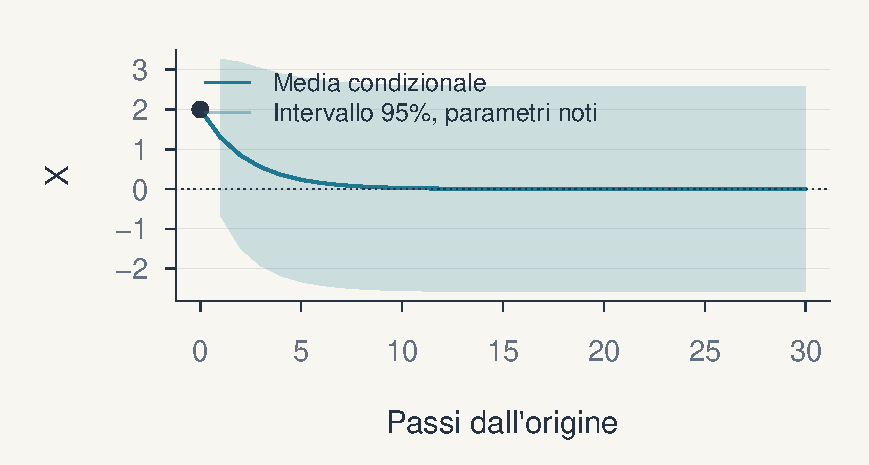
\includegraphics[width=9.85cm,height=5.25cm,keepaspectratio]{Risultati/Figure/16_AR1_previsione.pdf}
\vspace{1.5mm}
\PSmall{Esempio teorico: $\phi=0{,}65$, $\mu=0$, $X_T=2$, $\sigma=1$. Parametri noti.}
\[\widehat Y_{T+h\mid T}=\mu+\phi^h(Y_T-\mu)\]

\end{minipage}\end{lrbox}
\typeout{FULLBOX:026:PilotLeftBox:\the\ht\PilotLeftBox:\the\dp\PilotLeftBox}

\begin{lrbox}{\PilotRightBox}
\begin{minipage}[t]{7.55cm}\raggedright\color{Ink}\fontsize{11.3}{14.8}\selectfont
\PBody{Ogni nuovo passo moltiplica per $\phi$ lo scostamento residuo dalla media. Quando $|\phi|<1$, il contributo dell’ultima osservazione si attenua.}
\vspace{2.5mm}
\PInfo{Se $\phi<0$, il centro previsto alterna il segno dello scostamento. Se $\phi$ è vicino a 1, il ritorno è più lento.}
\PCode{R · ricorsione in forma chiusa}{026_esempio.R}
\end{minipage}\end{lrbox}
\typeout{FULLBOX:026:PilotRightBox:\the\ht\PilotRightBox:\the\dp\PilotRightBox}

\begin{tikzpicture}[remember picture,overlay]
\PilotChrome{La ricorsione porta la previsione verso la media}{III · MEMORIA E INNOVAZIONI}{26}{La previsione AR(1) stazionaria ricorda sempre meno il valore iniziale al crescere di $h$.}
\node[anchor=north west,inner sep=0] at([xshift=.96cm,yshift=-2.13cm]current page.north west){\usebox{\PilotLeftBox}};
\node[anchor=north west,inner sep=0] at([xshift=11.52cm,yshift=-2.13cm]current page.north west){\usebox{\PilotRightBox}};
\end{tikzpicture}\end{frame}

\begin{frame}[plain]\hypertarget{slide27}{}
\bookmark[level=1,page=27]{L’errore raccoglie gli shock non ancora osservati}
\begin{lrbox}{\TitleBox}
\begin{minipage}[t]{17.7cm}\raggedright\color{Ink}\fontsize{11.3}{14.8}\selectfont
\color{Navy}\bfseries\fontsize{20.6}{24.5}\selectfont L’errore raccoglie gli shock non ancora osservati
\end{minipage}\end{lrbox}
\typeout{FULLBOX:027:TitleBox:\the\ht\TitleBox:\the\dp\TitleBox}

\begin{lrbox}{\RecallBox}
\begin{minipage}[t]{14.3cm}\raggedright\color{Ink}\fontsize{11.3}{14.8}\selectfont
\fontsize{10.3}{13.8}\selectfont L’orizzonte aumenta il numero di innovazioni che la previsione non può conoscere.
\end{minipage}\end{lrbox}
\typeout{FULLBOX:027:RecallBox:\the\ht\RecallBox:\the\dp\RecallBox}

\begin{lrbox}{\PilotLeftBox}
\begin{minipage}[t]{10.05cm}\raggedright\color{Ink}\fontsize{11.3}{14.8}\selectfont
\[e_{T+h\mid T}=\sum_{j=0}^{h-1}\phi^j\varepsilon_{T+h-j}\]
{\fontsize{10.2}{13.1}\selectfont\renewcommand{\arraystretch}{1.45}\begin{tabular}{@{}p{2cm}p{7.1cm}@{}}\toprule
\textbf{Orizzonte} & \textbf{Innovazioni che entrano}\\\midrule
1 & $\varepsilon_{T+1}$\\
2 & $\varepsilon_{T+2}+\phi\varepsilon_{T+1}$\\
3 & $\varepsilon_{T+3}+\phi\varepsilon_{T+2}+\phi^2\varepsilon_{T+1}$\\
\bottomrule\end{tabular}}

\end{minipage}\end{lrbox}
\typeout{FULLBOX:027:PilotLeftBox:\the\ht\PilotLeftBox:\the\dp\PilotLeftBox}

\begin{lrbox}{\PilotRightBox}
\begin{minipage}[t]{7.55cm}\raggedright\color{Ink}\fontsize{11.3}{14.8}\selectfont
\PBody{Allungare l’orizzonte aggiunge nuove innovazioni. Gli shock più vicini all’origine vengono trasmessi attraverso potenze di $\phi$.}
\vspace{2.5mm}
\PInfo{La somma riguarda soltanto innovazioni successive a $T$. Con parametri noti, la storia osservata è già incorporata nel centro previsto.}
\PSmall{Il segno dell’errore adottato qui è sempre osservato meno previsto.}

\end{minipage}\end{lrbox}
\typeout{FULLBOX:027:PilotRightBox:\the\ht\PilotRightBox:\the\dp\PilotRightBox}

\begin{tikzpicture}[remember picture,overlay]
\PilotChrome{L’errore raccoglie gli shock non ancora osservati}{III · MEMORIA E INNOVAZIONI}{27}{L’orizzonte aumenta il numero di innovazioni che la previsione non può conoscere.}
\node[anchor=north west,inner sep=0] at([xshift=.96cm,yshift=-2.13cm]current page.north west){\usebox{\PilotLeftBox}};
\node[anchor=north west,inner sep=0] at([xshift=11.52cm,yshift=-2.13cm]current page.north west){\usebox{\PilotRightBox}};
\end{tikzpicture}\end{frame}

\begin{frame}[plain]\hypertarget{slide28}{}
\bookmark[level=1,page=28]{La varianza AR(1) cresce verso un limite}
\begin{lrbox}{\TitleBox}
\begin{minipage}[t]{17.7cm}\raggedright\color{Ink}\fontsize{11.3}{14.8}\selectfont
\color{Navy}\bfseries\fontsize{20.6}{24.5}\selectfont La varianza AR(1) cresce verso un limite
\end{minipage}\end{lrbox}
\typeout{FULLBOX:028:TitleBox:\the\ht\TitleBox:\the\dp\TitleBox}

\begin{lrbox}{\RecallBox}
\begin{minipage}[t]{14.3cm}\raggedright\color{Ink}\fontsize{11.3}{14.8}\selectfont
\fontsize{10.3}{13.8}\selectfont In un AR(1) stazionario, l’incertezza condizionata tende alla variabilità marginale del processo.
\end{minipage}\end{lrbox}
\typeout{FULLBOX:028:RecallBox:\the\ht\RecallBox:\the\dp\RecallBox}

\begin{lrbox}{\PilotLeftBox}
\begin{minipage}[t]{10.05cm}\raggedright\color{Ink}\fontsize{11.3}{14.8}\selectfont
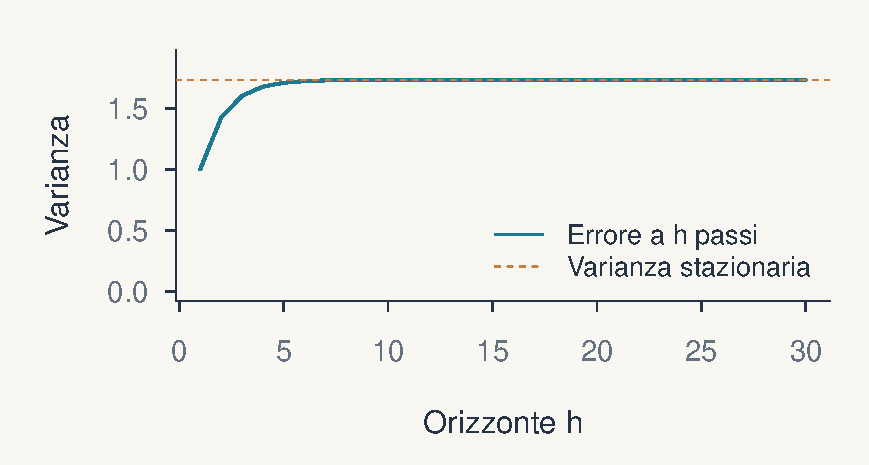
\includegraphics[width=9.85cm,height=5.25cm,keepaspectratio]{Risultati/Figure/17_AR1_varianza.pdf}
\vspace{1.5mm}
\PSmall{Parametri noti. Il limite coincide con la varianza stazionaria del processo.}
\[\operatorname{Var}(e_{T+h\mid T})=\sigma^2\frac{1-\phi^{2h}}{1-\phi^2}\]

\end{minipage}\end{lrbox}
\typeout{FULLBOX:028:PilotLeftBox:\the\ht\PilotLeftBox:\the\dp\PilotLeftBox}

\begin{lrbox}{\PilotRightBox}
\begin{minipage}[t]{7.55cm}\raggedright\color{Ink}\fontsize{11.3}{14.8}\selectfont
\PBody{Con innovazioni incorrelate, la varianza della somma è la somma delle varianze pesate. Per $|\phi|<1$, la serie geometrica converge.}
\vspace{2.5mm}
\PInfo{A un passo la varianza è $\sigma^2$. Per orizzonti lunghi tende a $\sigma^2/(1-\phi^2)$: non cresce senza limite come nel random walk.}
\PCode{R · varianza previsionale}{028_esempio.R}
\end{minipage}\end{lrbox}
\typeout{FULLBOX:028:PilotRightBox:\the\ht\PilotRightBox:\the\dp\PilotRightBox}

\begin{tikzpicture}[remember picture,overlay]
\PilotChrome{La varianza AR(1) cresce verso un limite}{III · MEMORIA E INNOVAZIONI}{28}{In un AR(1) stazionario, l’incertezza condizionata tende alla variabilità marginale del processo.}
\node[anchor=north west,inner sep=0] at([xshift=.96cm,yshift=-2.13cm]current page.north west){\usebox{\PilotLeftBox}};
\node[anchor=north west,inner sep=0] at([xshift=11.52cm,yshift=-2.13cm]current page.north west){\usebox{\PilotRightBox}};
\end{tikzpicture}\end{frame}

\begin{frame}[plain]\hypertarget{slide29}{}
\bookmark[level=1,page=29]{Il coefficiente cambia persistenza e oscillazione}
\begin{lrbox}{\TitleBox}
\begin{minipage}[t]{17.7cm}\raggedright\color{Ink}\fontsize{11.3}{14.8}\selectfont
\color{Navy}\bfseries\fontsize{20.6}{24.5}\selectfont Il coefficiente cambia persistenza e oscillazione
\end{minipage}\end{lrbox}
\typeout{FULLBOX:029:TitleBox:\the\ht\TitleBox:\the\dp\TitleBox}

\begin{lrbox}{\RecallBox}
\begin{minipage}[t]{14.3cm}\raggedright\color{Ink}\fontsize{11.3}{14.8}\selectfont
\fontsize{10.3}{13.8}\selectfont Persistenza elevata e non stazionarietà possono apparire simili in campioni brevi.
\end{minipage}\end{lrbox}
\typeout{FULLBOX:029:RecallBox:\the\ht\RecallBox:\the\dp\RecallBox}

\begin{lrbox}{\FullWideBox}
\begin{minipage}[t]{18.1cm}\raggedright\color{Ink}\fontsize{11.3}{14.8}\selectfont
\centering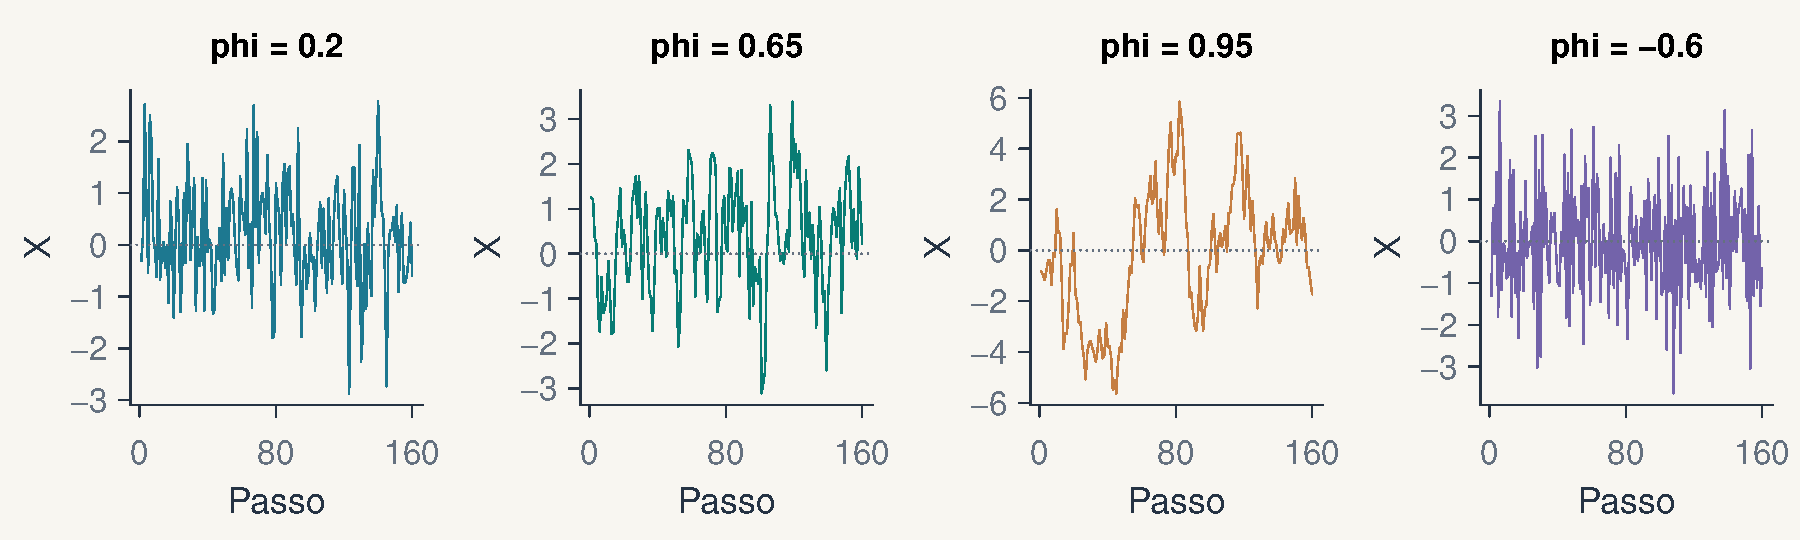
\includegraphics[width=18.05cm,height=5.8cm,keepaspectratio]{Risultati/Figure/14_AR1_traiettorie.pdf}
\end{minipage}\end{lrbox}
\typeout{FULLBOX:029:FullWideBox:\the\ht\FullWideBox:\the\dp\FullWideBox}

\begin{lrbox}{\PilotRightBox}
\begin{minipage}[t]{18.1cm}\raggedright\color{Ink}\fontsize{11.3}{14.8}\selectfont
\PBody{Simulazioni con innovazioni di varianza unitaria. Un coefficiente positivo alto produce persistenza; un coefficiente negativo produce alternanza. I percorsi sono simulati, con semi registrati.}
\end{minipage}\end{lrbox}
\typeout{FULLBOX:029:PilotRightBox:\the\ht\PilotRightBox:\the\dp\PilotRightBox}

\begin{tikzpicture}[remember picture,overlay]
\PilotChrome{Il coefficiente cambia persistenza e oscillazione}{III · MEMORIA E INNOVAZIONI}{29}{Persistenza elevata e non stazionarietà possono apparire simili in campioni brevi.}
\node[anchor=north west,inner sep=0] at([xshift=.96cm,yshift=-2.13cm]current page.north west){\usebox{\FullWideBox}};
\node[anchor=north west,inner sep=0] at([xshift=.96cm,yshift=-8.25cm]current page.north west){\usebox{\PilotRightBox}};
\end{tikzpicture}\end{frame}

\begin{frame}[plain]\hypertarget{slide30}{}
\bookmark[level=1,page=30]{L’autocorrelazione teorica segue le potenze di phi}
\begin{lrbox}{\TitleBox}
\begin{minipage}[t]{17.7cm}\raggedright\color{Ink}\fontsize{11.3}{14.8}\selectfont
\color{Navy}\bfseries\fontsize{20.6}{24.5}\selectfont L’autocorrelazione teorica segue le potenze di phi
\end{minipage}\end{lrbox}
\typeout{FULLBOX:030:TitleBox:\the\ht\TitleBox:\the\dp\TitleBox}

\begin{lrbox}{\RecallBox}
\begin{minipage}[t]{14.3cm}\raggedright\color{Ink}\fontsize{11.3}{14.8}\selectfont
\fontsize{10.3}{13.8}\selectfont La struttura teorica orienta l’interpretazione; l’incertezza campionaria resta visibile.
\end{minipage}\end{lrbox}
\typeout{FULLBOX:030:RecallBox:\the\ht\RecallBox:\the\dp\RecallBox}

\begin{lrbox}{\PilotLeftBox}
\begin{minipage}[t]{10.05cm}\raggedright\color{Ink}\fontsize{11.3}{14.8}\selectfont
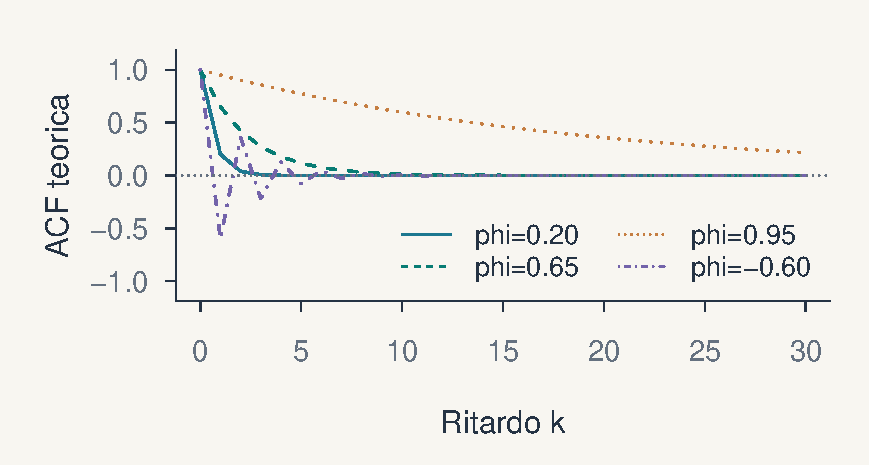
\includegraphics[width=9.85cm,height=5.25cm,keepaspectratio]{Risultati/Figure/15_AR1_ACF_teorica.pdf}
\vspace{1.5mm}
\PSmall{ACF esatte dei processi illustrati; non sono stime ottenute da un singolo campione.}
\[\rho(k)=\phi^{|k|}\]

\end{minipage}\end{lrbox}
\typeout{FULLBOX:030:PilotLeftBox:\the\ht\PilotLeftBox:\the\dp\PilotLeftBox}

\begin{lrbox}{\PilotRightBox}
\begin{minipage}[t]{7.55cm}\raggedright\color{Ink}\fontsize{11.3}{14.8}\selectfont
\PBody{Per $\phi>0$ la correlazione decresce mantenendo il segno. Per $\phi<0$ il segno alterna. Il modulo determina la velocità di attenuazione.}
\vspace{2.5mm}
\PInfo{L’ACF campionaria oscilla attorno alla forma teorica. Un grafico campionario non deve coincidere punto per punto con questa curva.}
\PCode{R · ACF teorica}{030_esempio.R}
\end{minipage}\end{lrbox}
\typeout{FULLBOX:030:PilotRightBox:\the\ht\PilotRightBox:\the\dp\PilotRightBox}

\begin{tikzpicture}[remember picture,overlay]
\PilotChrome{L’autocorrelazione teorica segue le potenze di phi}{III · MEMORIA E INNOVAZIONI}{30}{La struttura teorica orienta l’interpretazione; l’incertezza campionaria resta visibile.}
\node[anchor=north west,inner sep=0] at([xshift=.96cm,yshift=-2.13cm]current page.north west){\usebox{\PilotLeftBox}};
\node[anchor=north west,inner sep=0] at([xshift=11.52cm,yshift=-2.13cm]current page.north west){\usebox{\PilotRightBox}};
\end{tikzpicture}\end{frame}

\begin{frame}[plain]\hypertarget{slide31}{}
\bookmark[level=1,page=31]{Un AR(p) usa più ritardi della stessa serie}
\begin{lrbox}{\TitleBox}
\begin{minipage}[t]{17.7cm}\raggedright\color{Ink}\fontsize{11.3}{14.8}\selectfont
\color{Navy}\bfseries\fontsize{20.6}{24.5}\selectfont Un AR(p) usa più ritardi della stessa serie
\end{minipage}\end{lrbox}
\typeout{FULLBOX:031:TitleBox:\the\ht\TitleBox:\the\dp\TitleBox}

\begin{lrbox}{\RecallBox}
\begin{minipage}[t]{14.3cm}\raggedright\color{Ink}\fontsize{11.3}{14.8}\selectfont
\fontsize{10.3}{13.8}\selectfont Negli AR di ordine superiore la condizione corretta riguarda tutte le radici del polinomio.
\end{minipage}\end{lrbox}
\typeout{FULLBOX:031:RecallBox:\the\ht\RecallBox:\the\dp\RecallBox}

\begin{lrbox}{\PilotLeftBox}
\begin{minipage}[t]{10.05cm}\raggedright\color{Ink}\fontsize{11.3}{14.8}\selectfont
\[X_t=\phi_1X_{t-1}+\cdots+\phi_pX_{t-p}+\varepsilon_t\]
\[\phi(B)X_t=\varepsilon_t,\qquad\phi(z)=1-\sum_{j=1}^p\phi_jz^j\]
\PInfo{L’operatore di ritardo soddisfa $BX_t=X_{t-1}$. Le radici del polinomio descrivono la stabilità della ricorrenza.}

\end{minipage}\end{lrbox}
\typeout{FULLBOX:031:PilotLeftBox:\the\ht\PilotLeftBox:\the\dp\PilotLeftBox}

\begin{lrbox}{\PilotRightBox}
\begin{minipage}[t]{7.55cm}\raggedright\color{Ink}\fontsize{11.3}{14.8}\selectfont
\PBody{I coefficienti pesano ritardi diversi. La somma dei coefficienti, da sola, non è un controllo generale della stazionarietà per ogni ordine.}
\vspace{2.5mm}
\PBody{Per un AR causale stazionario tutte le radici di $\phi(z)=0$ devono stare fuori dal cerchio unitario.}
\vspace{2.5mm}

\end{minipage}\end{lrbox}
\typeout{FULLBOX:031:PilotRightBox:\the\ht\PilotRightBox:\the\dp\PilotRightBox}

\begin{tikzpicture}[remember picture,overlay]
\PilotChrome{Un AR(p) usa più ritardi della stessa serie}{III · MEMORIA E INNOVAZIONI}{31}{Negli AR di ordine superiore la condizione corretta riguarda tutte le radici del polinomio.}
\node[anchor=north west,inner sep=0] at([xshift=.96cm,yshift=-2.13cm]current page.north west){\usebox{\PilotLeftBox}};
\node[anchor=north west,inner sep=0] at([xshift=11.52cm,yshift=-2.13cm]current page.north west){\usebox{\PilotRightBox}};
\end{tikzpicture}\end{frame}

\begin{frame}[plain]\hypertarget{slide32}{}
\bookmark[level=1,page=32]{Le radici AR devono stare fuori dal cerchio unitario}
\begin{lrbox}{\TitleBox}
\begin{minipage}[t]{17.7cm}\raggedright\color{Ink}\fontsize{11.3}{14.8}\selectfont
\color{Navy}\bfseries\fontsize{20.6}{24.5}\selectfont Le radici AR devono stare fuori dal cerchio unitario
\end{minipage}\end{lrbox}
\typeout{FULLBOX:032:TitleBox:\the\ht\TitleBox:\the\dp\TitleBox}

\begin{lrbox}{\RecallBox}
\begin{minipage}[t]{14.3cm}\raggedright\color{Ink}\fontsize{11.3}{14.8}\selectfont
\fontsize{10.3}{13.8}\selectfont Radici AR fuori dal cerchio unitario corrispondono a una dinamica causale stazionaria.
\end{minipage}\end{lrbox}
\typeout{FULLBOX:032:RecallBox:\the\ht\RecallBox:\the\dp\RecallBox}

\begin{lrbox}{\PilotLeftBox}
\begin{minipage}[t]{10.05cm}\raggedright\color{Ink}\fontsize{11.3}{14.8}\selectfont
\begin{tikzpicture}[x=1cm,y=1cm]
\path[use as bounding box](-.1,-.15) rectangle(9.7,5.1);
\draw[pAxis](1,2.5)--(8.5,2.5)node[right,pNote]{Re};
\draw[pAxis](4.7,.35)--(4.7,4.7)node[above,pNote]{Im};
\draw[Classical,line width=1pt](4.7,2.5)circle(1.55);
\node[pNote]at(5.6,3.85){$|z|=1$};\fill[GeoB](7.283,2.5)circle(3.2pt);\node[pLabel]at(7.283,1.85){$z=1/0{,}6$};
\end{tikzpicture}
\[1-0{,}6z=0\quad\Longrightarrow\quad z=1/0{,}6\]

\end{minipage}\end{lrbox}
\typeout{FULLBOX:032:PilotLeftBox:\the\ht\PilotLeftBox:\the\dp\PilotLeftBox}

\begin{lrbox}{\PilotRightBox}
\begin{minipage}[t]{7.55cm}\raggedright\color{Ink}\fontsize{11.3}{14.8}\selectfont
\PBody{Il disegno mostra un AR(1) con $\phi=0{,}6$. La radice è circa $1{,}67$ e ha modulo maggiore di uno.}
\vspace{2.5mm}
\PInfo{Per un AR(2), polyroot riceve i coefficienti in ordine di potenza crescente: costante, termine in $z$, termine in $z^2$.}
\PCode{R · controllo per un AR(2)}{032_esempio.R}
\end{minipage}\end{lrbox}
\typeout{FULLBOX:032:PilotRightBox:\the\ht\PilotRightBox:\the\dp\PilotRightBox}

\begin{tikzpicture}[remember picture,overlay]
\PilotChrome{Le radici AR devono stare fuori dal cerchio unitario}{III · MEMORIA E INNOVAZIONI}{32}{Radici AR fuori dal cerchio unitario corrispondono a una dinamica causale stazionaria.}
\node[anchor=north west,inner sep=0] at([xshift=.96cm,yshift=-2.13cm]current page.north west){\usebox{\PilotLeftBox}};
\node[anchor=north west,inner sep=0] at([xshift=11.52cm,yshift=-2.13cm]current page.north west){\usebox{\PilotRightBox}};
\end{tikzpicture}\end{frame}

\begin{frame}[plain]\hypertarget{slide33}{}
\bookmark[level=1,page=33]{Un MA(1) combina innovazioni, non osservazioni}
\begin{lrbox}{\TitleBox}
\begin{minipage}[t]{17.7cm}\raggedright\color{Ink}\fontsize{11.3}{14.8}\selectfont
\color{Navy}\bfseries\fontsize{20.6}{24.5}\selectfont Un MA(1) combina innovazioni, non osservazioni
\end{minipage}\end{lrbox}
\typeout{FULLBOX:033:TitleBox:\the\ht\TitleBox:\the\dp\TitleBox}

\begin{lrbox}{\RecallBox}
\begin{minipage}[t]{14.3cm}\raggedright\color{Ink}\fontsize{11.3}{14.8}\selectfont
\fontsize{10.3}{13.8}\selectfont Nel modello MA si mediano shock latenti; una media mobile descrittiva combina dati osservati.
\end{minipage}\end{lrbox}
\typeout{FULLBOX:033:RecallBox:\the\ht\RecallBox:\the\dp\RecallBox}

\begin{lrbox}{\PilotLeftBox}
\begin{minipage}[t]{10.05cm}\raggedright\color{Ink}\fontsize{11.3}{14.8}\selectfont
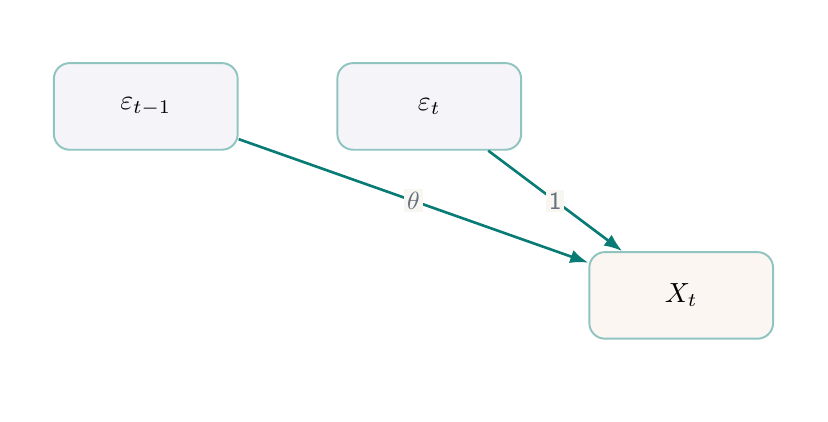
\begin{tikzpicture}[x=1cm,y=1cm]
\path[use as bounding box](-.1,-.15) rectangle(9.7,4.5);
\node[pFlow,text width=2.1cm,fill=GeoC!7] (a) at(1.4,3.5){$\varepsilon_{t-1}$};
\node[pFlow,text width=2.1cm,fill=GeoC!7] (b) at(5.0,3.5){$\varepsilon_t$};
\node[pFlow,text width=2.1cm,fill=GeoB!7] (c) at(8.2,1.1){$X_t$};
\draw[pEdge] (a) -- node[pNote,fill=Paper,inner sep=1pt]{$\theta$} (c);
\draw[pEdge] (b) -- node[pNote,fill=Paper,inner sep=1pt]{1} (c);
\end{tikzpicture}
\[X_t=\varepsilon_t+\theta\varepsilon_{t-1}\]

\end{minipage}\end{lrbox}
\typeout{FULLBOX:033:PilotLeftBox:\the\ht\PilotLeftBox:\the\dp\PilotLeftBox}

\begin{lrbox}{\PilotRightBox}
\begin{minipage}[t]{7.55cm}\raggedright\color{Ink}\fontsize{11.3}{14.8}\selectfont
\PBody{Il termine moving average indica una combinazione di innovazioni presenti e passate. Non è una media mobile usata per lisciare i dati.}
\vspace{2.5mm}
\PInfo{Adottiamo il segno positivo della convenzione R. Le innovazioni hanno media nulla, varianza $\sigma^2$ e sono incorrelate nel tempo.}
\PCode{R · simulare un MA(1)}{033_esempio.R}
\end{minipage}\end{lrbox}
\typeout{FULLBOX:033:PilotRightBox:\the\ht\PilotRightBox:\the\dp\PilotRightBox}

\begin{tikzpicture}[remember picture,overlay]
\PilotChrome{Un MA(1) combina innovazioni, non osservazioni}{III · MEMORIA E INNOVAZIONI}{33}{Nel modello MA si mediano shock latenti; una media mobile descrittiva combina dati osservati.}
\node[anchor=north west,inner sep=0] at([xshift=.96cm,yshift=-2.13cm]current page.north west){\usebox{\PilotLeftBox}};
\node[anchor=north west,inner sep=0] at([xshift=11.52cm,yshift=-2.13cm]current page.north west){\usebox{\PilotRightBox}};
\end{tikzpicture}\end{frame}

\begin{frame}[plain]\hypertarget{slide34}{}
\bookmark[level=1,page=34]{L’ACF di un MA(1) si annulla oltre il primo ritardo}
\begin{lrbox}{\TitleBox}
\begin{minipage}[t]{17.7cm}\raggedright\color{Ink}\fontsize{11.3}{14.8}\selectfont
\color{Navy}\bfseries\fontsize{20.6}{24.5}\selectfont L’ACF di un MA(1) si annulla oltre il primo ritardo
\end{minipage}\end{lrbox}
\typeout{FULLBOX:034:TitleBox:\the\ht\TitleBox:\the\dp\TitleBox}

\begin{lrbox}{\RecallBox}
\begin{minipage}[t]{14.3cm}\raggedright\color{Ink}\fontsize{11.3}{14.8}\selectfont
\fontsize{10.3}{13.8}\selectfont Il taglio teorico dell’ACF non elimina le fluttuazioni della sua stima campionaria.
\end{minipage}\end{lrbox}
\typeout{FULLBOX:034:RecallBox:\the\ht\RecallBox:\the\dp\RecallBox}

\begin{lrbox}{\PilotLeftBox}
\begin{minipage}[t]{10.05cm}\raggedright\color{Ink}\fontsize{11.3}{14.8}\selectfont
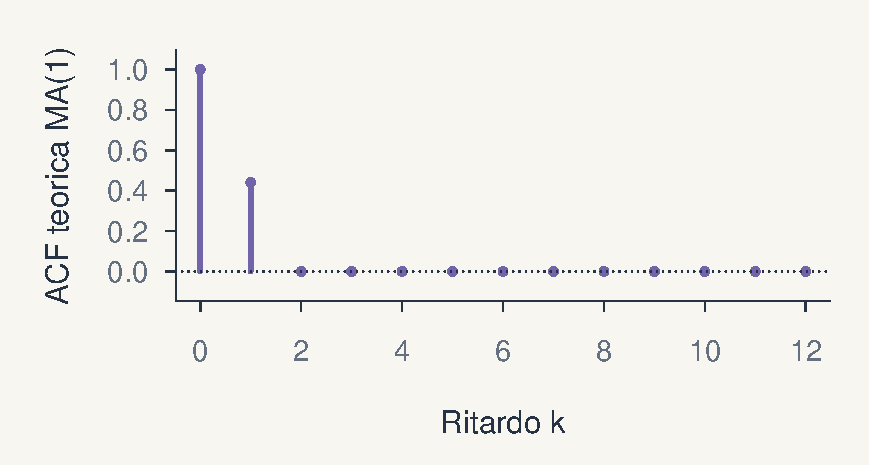
\includegraphics[width=9.85cm,height=5.25cm,keepaspectratio]{Risultati/Figure/18_MA1_ACF.pdf}
\vspace{1.5mm}
\PSmall{ACF teorica per $\theta=0{,}6$.}
\[\rho(1)=\frac{\theta}{1+\theta^2},\qquad\rho(k)=0\ \ (|k|>1)\]

\end{minipage}\end{lrbox}
\typeout{FULLBOX:034:PilotLeftBox:\the\ht\PilotLeftBox:\the\dp\PilotLeftBox}

\begin{lrbox}{\PilotRightBox}
\begin{minipage}[t]{7.55cm}\raggedright\color{Ink}\fontsize{11.3}{14.8}\selectfont
\PBody{Due valori consecutivi condividono un’innovazione. Valori separati da più di un passo non condividono innovazioni in questo modello.}
\vspace{2.5mm}
\PInfo{La proprietà di taglio vale per l’ACF teorica. Le correlazioni campionarie ai ritardi successivi non sono esattamente zero.}
\PCode{R · ACF MA(1)}{034_esempio.R}
\end{minipage}\end{lrbox}
\typeout{FULLBOX:034:PilotRightBox:\the\ht\PilotRightBox:\the\dp\PilotRightBox}

\begin{tikzpicture}[remember picture,overlay]
\PilotChrome{L’ACF di un MA(1) si annulla oltre il primo ritardo}{III · MEMORIA E INNOVAZIONI}{34}{Il taglio teorico dell’ACF non elimina le fluttuazioni della sua stima campionaria.}
\node[anchor=north west,inner sep=0] at([xshift=.96cm,yshift=-2.13cm]current page.north west){\usebox{\PilotLeftBox}};
\node[anchor=north west,inner sep=0] at([xshift=11.52cm,yshift=-2.13cm]current page.north west){\usebox{\PilotRightBox}};
\end{tikzpicture}\end{frame}

\begin{frame}[plain]\hypertarget{slide35}{}
\bookmark[level=1,page=35]{Invertire un MA permette di ricostruire gli shock}
\begin{lrbox}{\TitleBox}
\begin{minipage}[t]{17.7cm}\raggedright\color{Ink}\fontsize{11.3}{14.8}\selectfont
\color{Navy}\bfseries\fontsize{20.6}{24.5}\selectfont Invertire un MA permette di ricostruire gli shock
\end{minipage}\end{lrbox}
\typeout{FULLBOX:035:TitleBox:\the\ht\TitleBox:\the\dp\TitleBox}

\begin{lrbox}{\RecallBox}
\begin{minipage}[t]{14.3cm}\raggedright\color{Ink}\fontsize{11.3}{14.8}\selectfont
\fontsize{10.3}{13.8}\selectfont La condizione sulle radici MA sceglie una rappresentazione degli shock recuperabile dal passato.
\end{minipage}\end{lrbox}
\typeout{FULLBOX:035:RecallBox:\the\ht\RecallBox:\the\dp\RecallBox}

\begin{lrbox}{\PilotLeftBox}
\begin{minipage}[t]{10.05cm}\raggedright\color{Ink}\fontsize{11.3}{14.8}\selectfont
\begin{tikzpicture}[x=1cm,y=1cm]
\path[use as bounding box](-.1,-.15) rectangle(9.7,5.1);
\draw[pAxis](1,2.5)--(8.5,2.5)node[right,pNote]{Re};
\draw[pAxis](4.7,.35)--(4.7,4.7)node[above,pNote]{Im};
\draw[Classical,line width=1pt](4.7,2.5)circle(1.55);
\node[pNote]at(5.6,3.85){$|z|=1$};\fill[GeoB](2.117,2.5)circle(3.2pt);\node[pLabel]at(2.117,1.85){$z=-1/0{,}6$};
\end{tikzpicture}
\[\theta(z)=1+\theta z,\qquad |z_{\mathrm{radice}}|>1\]

\end{minipage}\end{lrbox}
\typeout{FULLBOX:035:PilotLeftBox:\the\ht\PilotLeftBox:\the\dp\PilotLeftBox}

\begin{lrbox}{\PilotRightBox}
\begin{minipage}[t]{7.55cm}\raggedright\color{Ink}\fontsize{11.3}{14.8}\selectfont
\PBody{L’invertibilità consente di esprimere le innovazioni mediante una combinazione stabile della storia osservata. Per MA(1) richiede $|\theta|<1$.}
\vspace{2.5mm}
\PInfo{Stazionarietà e invertibilità sono proprietà diverse: un MA finito è stazionario sotto le ipotesi sulle innovazioni, anche quando non è invertibile.}
\PCode{R · invertibilità MA(1)}{035_esempio.R}
\end{minipage}\end{lrbox}
\typeout{FULLBOX:035:PilotRightBox:\the\ht\PilotRightBox:\the\dp\PilotRightBox}

\begin{tikzpicture}[remember picture,overlay]
\PilotChrome{Invertire un MA permette di ricostruire gli shock}{III · MEMORIA E INNOVAZIONI}{35}{La condizione sulle radici MA sceglie una rappresentazione degli shock recuperabile dal passato.}
\node[anchor=north west,inner sep=0] at([xshift=.96cm,yshift=-2.13cm]current page.north west){\usebox{\PilotLeftBox}};
\node[anchor=north west,inner sep=0] at([xshift=11.52cm,yshift=-2.13cm]current page.north west){\usebox{\PilotRightBox}};
\end{tikzpicture}\end{frame}

\begin{frame}[plain]\hypertarget{slide36}{}
\bookmark[level=1,page=36]{Nel MA(1) la memoria predittiva diretta è breve}
\begin{lrbox}{\TitleBox}
\begin{minipage}[t]{17.7cm}\raggedright\color{Ink}\fontsize{11.3}{14.8}\selectfont
\color{Navy}\bfseries\fontsize{20.6}{24.5}\selectfont Nel MA(1) la memoria predittiva diretta è breve
\end{minipage}\end{lrbox}
\typeout{FULLBOX:036:TitleBox:\the\ht\TitleBox:\the\dp\TitleBox}

\begin{lrbox}{\RecallBox}
\begin{minipage}[t]{14.3cm}\raggedright\color{Ink}\fontsize{11.3}{14.8}\selectfont
\fontsize{10.3}{13.8}\selectfont Una memoria predittiva finita può convivere con una variabilità futura non nulla.
\end{minipage}\end{lrbox}
\typeout{FULLBOX:036:RecallBox:\the\ht\RecallBox:\the\dp\RecallBox}

\begin{lrbox}{\PilotLeftBox}
\begin{minipage}[t]{10.05cm}\raggedright\color{Ink}\fontsize{11.3}{14.8}\selectfont
\[\widehat X_{T+1\mid T}=\theta\varepsilon_T\]
\[\widehat X_{T+h\mid T}=0\quad (h\geq2)\]
\PInfo{Queste formule assumono innovazioni ricostruite dalla storia e parametri noti. Con un campione finito, l’inizializzazione introduce una differenza pratica.}

\end{minipage}\end{lrbox}
\typeout{FULLBOX:036:PilotLeftBox:\the\ht\PilotLeftBox:\the\dp\PilotLeftBox}

\begin{lrbox}{\PilotRightBox}
\begin{minipage}[t]{7.55cm}\raggedright\color{Ink}\fontsize{11.3}{14.8}\selectfont
\PBody{A un passo rimane lo shock noto all’origine. A due o più passi entrano soltanto innovazioni future, la cui media condizionata è zero.}
\vspace{2.5mm}
\PBody{L’incertezza rimane: la varianza passa da $\sigma^2$ a $\sigma^2(1+\theta^2)$. Una previsione media nulla non significa processo costante.}
\vspace{2.5mm}

\end{minipage}\end{lrbox}
\typeout{FULLBOX:036:PilotRightBox:\the\ht\PilotRightBox:\the\dp\PilotRightBox}

\begin{tikzpicture}[remember picture,overlay]
\PilotChrome{Nel MA(1) la memoria predittiva diretta è breve}{III · MEMORIA E INNOVAZIONI}{36}{Una memoria predittiva finita può convivere con una variabilità futura non nulla.}
\node[anchor=north west,inner sep=0] at([xshift=.96cm,yshift=-2.13cm]current page.north west){\usebox{\PilotLeftBox}};
\node[anchor=north west,inner sep=0] at([xshift=11.52cm,yshift=-2.13cm]current page.north west){\usebox{\PilotRightBox}};
\end{tikzpicture}\end{frame}

\begin{frame}[plain]\hypertarget{slide37}{}
\bookmark[level=1,page=37]{ARMA combina propagazione e shock ritardati}
\begin{lrbox}{\TitleBox}
\begin{minipage}[t]{17.7cm}\raggedright\color{Ink}\fontsize{11.3}{14.8}\selectfont
\color{Navy}\bfseries\fontsize{20.6}{24.5}\selectfont ARMA combina propagazione e shock ritardati
\end{minipage}\end{lrbox}
\typeout{FULLBOX:037:TitleBox:\the\ht\TitleBox:\the\dp\TitleBox}

\begin{lrbox}{\RecallBox}
\begin{minipage}[t]{14.3cm}\raggedright\color{Ink}\fontsize{11.3}{14.8}\selectfont
\fontsize{10.3}{13.8}\selectfont La struttura ARMA descrive la dipendenza dopo che il livello e la stagione sono stati trattati.
\end{minipage}\end{lrbox}
\typeout{FULLBOX:037:RecallBox:\the\ht\RecallBox:\the\dp\RecallBox}

\begin{lrbox}{\PilotLeftBox}
\begin{minipage}[t]{10.05cm}\raggedright\color{Ink}\fontsize{11.3}{14.8}\selectfont
\[\phi(B)X_t=\theta(B)\varepsilon_t\]
\[X_t=\phi X_{t-1}+\varepsilon_t+\theta\varepsilon_{t-1}\]
{\fontsize{10.2}{13.1}\selectfont\renewcommand{\arraystretch}{1.45}\begin{tabular}{@{}p{2.5cm}p{6.6cm}@{}}\toprule
\textbf{Componente} & \textbf{Informazione rappresentata}\\\midrule
AR & Valori passati e propagazione\\
MA & Innovazioni passate e correzioni\\
\bottomrule\end{tabular}}

\end{minipage}\end{lrbox}
\typeout{FULLBOX:037:PilotLeftBox:\the\ht\PilotLeftBox:\the\dp\PilotLeftBox}

\begin{lrbox}{\PilotRightBox}
\begin{minipage}[t]{7.55cm}\raggedright\color{Ink}\fontsize{11.3}{14.8}\selectfont
\PBody{Un ARMA(1,1) unisce le due strutture. Le condizioni per una rappresentazione causale e invertibile si applicano ai rispettivi polinomi.}
\vspace{2.5mm}
\PInfo{AR e MA possono produrre ACF simili su campioni brevi. L’identificazione richiede confronto, parsimonia e verifica.}
\PCode{R · processo ARMA(1,1)}{037_esempio.R}
\end{minipage}\end{lrbox}
\typeout{FULLBOX:037:PilotRightBox:\the\ht\PilotRightBox:\the\dp\PilotRightBox}

\begin{tikzpicture}[remember picture,overlay]
\PilotChrome{ARMA combina propagazione e shock ritardati}{III · MEMORIA E INNOVAZIONI}{37}{La struttura ARMA descrive la dipendenza dopo che il livello e la stagione sono stati trattati.}
\node[anchor=north west,inner sep=0] at([xshift=.96cm,yshift=-2.13cm]current page.north west){\usebox{\PilotLeftBox}};
\node[anchor=north west,inner sep=0] at([xshift=11.52cm,yshift=-2.13cm]current page.north west){\usebox{\PilotRightBox}};
\end{tikzpicture}\end{frame}

\begin{frame}[plain]\hypertarget{slide38}{}
\bookmark[level=1,page=38]{La risposta a un impulso rende visibile la memoria}
\begin{lrbox}{\TitleBox}
\begin{minipage}[t]{17.7cm}\raggedright\color{Ink}\fontsize{11.3}{14.8}\selectfont
\color{Navy}\bfseries\fontsize{20.6}{24.5}\selectfont La risposta a un impulso rende visibile la memoria
\end{minipage}\end{lrbox}
\typeout{FULLBOX:038:TitleBox:\the\ht\TitleBox:\the\dp\TitleBox}

\begin{lrbox}{\RecallBox}
\begin{minipage}[t]{14.3cm}\raggedright\color{Ink}\fontsize{11.3}{14.8}\selectfont
\fontsize{10.3}{13.8}\selectfont La durata dell’effetto di un’innovazione spiega la forma della memoria previsionale.
\end{minipage}\end{lrbox}
\typeout{FULLBOX:038:RecallBox:\the\ht\RecallBox:\the\dp\RecallBox}

\begin{lrbox}{\PilotLeftBox}
\begin{minipage}[t]{10.05cm}\raggedright\color{Ink}\fontsize{11.3}{14.8}\selectfont
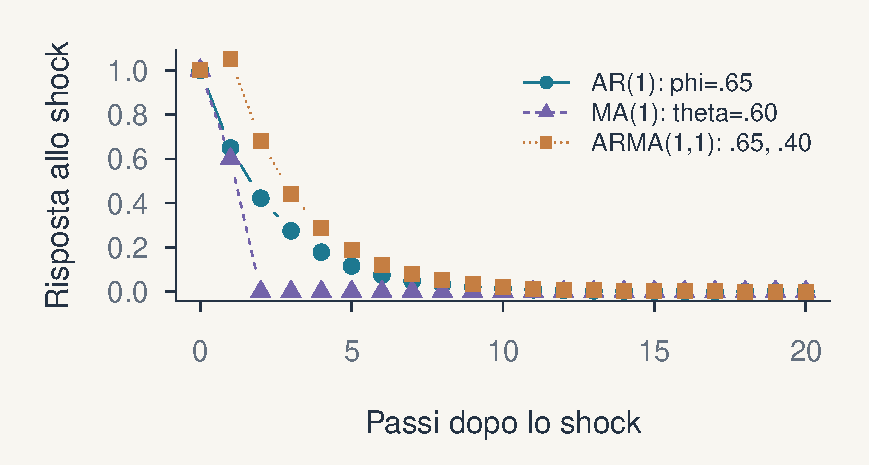
\includegraphics[width=9.85cm,height=4.75cm,keepaspectratio]{Risultati/Figure/19_risposta_impulso.pdf}
\vspace{1.5mm}
\PSmall{Risposte teoriche a un’innovazione unitaria: AR(1), MA(1) e ARMA(1,1).}
\[X_t=\sum_{j=0}^{\infty}\psi_j\varepsilon_{t-j}\]

\end{minipage}\end{lrbox}
\typeout{FULLBOX:038:PilotLeftBox:\the\ht\PilotLeftBox:\the\dp\PilotLeftBox}

\begin{lrbox}{\PilotRightBox}
\begin{minipage}[t]{7.55cm}\raggedright\color{Ink}\fontsize{11.3}{14.8}\selectfont
\PBody{I coefficienti $\psi_j$ descrivono quanto resta di uno shock dopo $j$ passi. Nel MA finito la risposta termina; nell’AR causale si attenua nel tempo.}
\vspace{2.5mm}
\PInfo{La rappresentazione è lineare e riferita al modello. Non attribuisce automaticamente allo shock un significato fisico causale.}
\PCode{R · pesi della risposta}{038_esempio.R}
\end{minipage}\end{lrbox}
\typeout{FULLBOX:038:PilotRightBox:\the\ht\PilotRightBox:\the\dp\PilotRightBox}

\begin{tikzpicture}[remember picture,overlay]
\PilotChrome{La risposta a un impulso rende visibile la memoria}{III · MEMORIA E INNOVAZIONI}{38}{La durata dell’effetto di un’innovazione spiega la forma della memoria previsionale.}
\node[anchor=north west,inner sep=0] at([xshift=.96cm,yshift=-2.13cm]current page.north west){\usebox{\PilotLeftBox}};
\node[anchor=north west,inner sep=0] at([xshift=11.52cm,yshift=-2.13cm]current page.north west){\usebox{\PilotRightBox}};
\end{tikzpicture}\end{frame}

\begin{frame}[plain]\hypertarget{slide39}{}
\bookmark[level=1,page=39]{ACF e PACF suggeriscono ipotesi da verificare}
\begin{lrbox}{\TitleBox}
\begin{minipage}[t]{17.7cm}\raggedright\color{Ink}\fontsize{11.3}{14.8}\selectfont
\color{Navy}\bfseries\fontsize{20.6}{24.5}\selectfont ACF e PACF suggeriscono ipotesi da verificare
\end{minipage}\end{lrbox}
\typeout{FULLBOX:039:TitleBox:\the\ht\TitleBox:\the\dp\TitleBox}

\begin{lrbox}{\RecallBox}
\begin{minipage}[t]{14.3cm}\raggedright\color{Ink}\fontsize{11.3}{14.8}\selectfont
\fontsize{10.3}{13.8}\selectfont L’identificazione propone una struttura; diagnostica e validazione ne valutano l’utilità.
\end{minipage}\end{lrbox}
\typeout{FULLBOX:039:RecallBox:\the\ht\RecallBox:\the\dp\RecallBox}

\begin{lrbox}{\PilotLeftBox}
\begin{minipage}[t]{10.05cm}\raggedright\color{Ink}\fontsize{11.3}{14.8}\selectfont
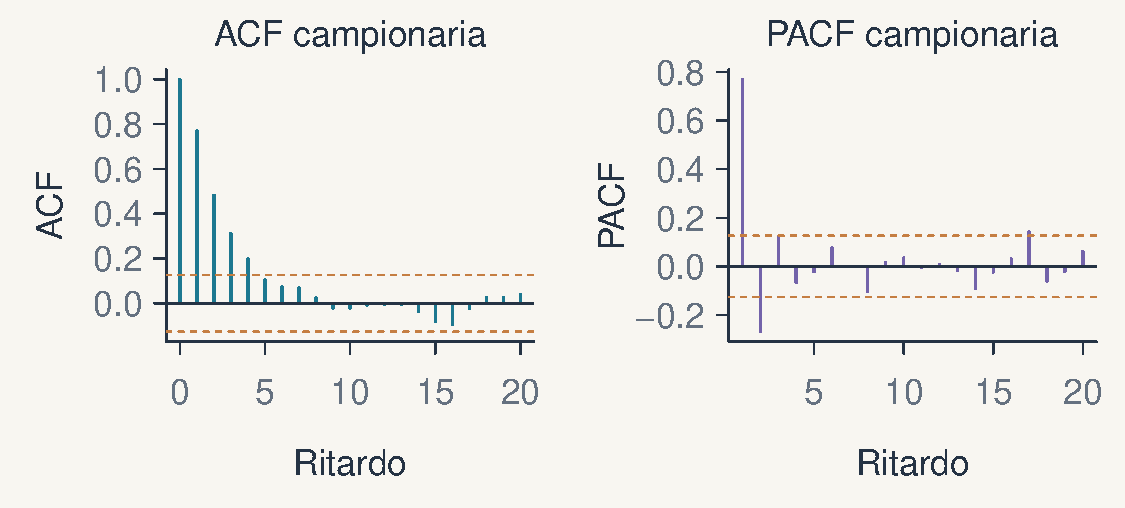
\includegraphics[width=9.85cm,height=5.25cm,keepaspectratio]{Risultati/Figure/20_ARMA_ACF_PACF.pdf}
\vspace{1.5mm}
\PSmall{Esempio simulato ARMA(1,1): entrambe le funzioni possono attenuarsi gradualmente.}

\end{minipage}\end{lrbox}
\typeout{FULLBOX:039:PilotLeftBox:\the\ht\PilotLeftBox:\the\dp\PilotLeftBox}

\begin{lrbox}{\PilotRightBox}
\begin{minipage}[t]{7.55cm}\raggedright\color{Ink}\fontsize{11.3}{14.8}\selectfont
\PBody{Per un AR puro la PACF teorica si interrompe dopo l’ordine; per un MA puro si interrompe l’ACF. In una combinazione ARMA entrambe possono avere una coda.}
\vspace{2.5mm}
\PInfo{Su dati reali, tendenza, stagione, campione breve e rumore alterano la leggibilità di questi indizi.}
\PBody{I grafici orientano una piccola famiglia di candidati. Non sono un algoritmo infallibile per scegliere un modello.}
\vspace{2.5mm}

\end{minipage}\end{lrbox}
\typeout{FULLBOX:039:PilotRightBox:\the\ht\PilotRightBox:\the\dp\PilotRightBox}

\begin{tikzpicture}[remember picture,overlay]
\PilotChrome{ACF e PACF suggeriscono ipotesi da verificare}{III · MEMORIA E INNOVAZIONI}{39}{L’identificazione propone una struttura; diagnostica e validazione ne valutano l’utilità.}
\node[anchor=north west,inner sep=0] at([xshift=.96cm,yshift=-2.13cm]current page.north west){\usebox{\PilotLeftBox}};
\node[anchor=north west,inner sep=0] at([xshift=11.52cm,yshift=-2.13cm]current page.north west){\usebox{\PilotRightBox}};
\end{tikzpicture}\end{frame}

\begin{frame}[plain]\hypertarget{slide40}{}
\bookmark[level=0,page=40]{IV · ARIMA E STAGIONE}
\bookmark[level=1,page=40]{ARIMA modella la dipendenza dopo le differenze}
\begin{lrbox}{\TitleBox}
\begin{minipage}[t]{17.7cm}\raggedright\color{Ink}\fontsize{11.3}{14.8}\selectfont
\color{Navy}\bfseries\fontsize{20.6}{24.5}\selectfont ARIMA modella la dipendenza dopo le differenze
\end{minipage}\end{lrbox}
\typeout{FULLBOX:040:TitleBox:\the\ht\TitleBox:\the\dp\TitleBox}

\begin{lrbox}{\RecallBox}
\begin{minipage}[t]{14.3cm}\raggedright\color{Ink}\fontsize{11.3}{14.8}\selectfont
\fontsize{10.3}{13.8}\selectfont ARIMA applica una struttura ARMA alla serie trasformata dalle differenze.
\end{minipage}\end{lrbox}
\typeout{FULLBOX:040:RecallBox:\the\ht\RecallBox:\the\dp\RecallBox}

\begin{lrbox}{\PilotLeftBox}
\begin{minipage}[t]{10.05cm}\raggedright\color{Ink}\fontsize{11.3}{14.8}\selectfont
\begin{tikzpicture}[x=1cm,y=1cm]
\path[use as bounding box](-.1,-.15) rectangle(9.7,4.8);
\node[pFlow,text width=3.4cm,fill=GeoA!7] (a) at(2.1,3.7){Serie in livelli\\$Y_t$};
\node[pFlow,text width=3.7cm,fill=GeoB!7] (b) at(7.3,3.7){Differenze\\$W_t=(1-B)^dY_t$};
\node[pFlow,text width=3.7cm,fill=GeoC!7] (c) at(7.3,1.1){Modello ARMA\\per $W_t$};
\draw[pEdge] (a) -- (b);
\draw[pEdge] (b) -- (c);
\end{tikzpicture}
\[\phi(B)(1-B)^dY_t=\theta(B)\varepsilon_t\]

\end{minipage}\end{lrbox}
\typeout{FULLBOX:040:PilotLeftBox:\the\ht\PilotLeftBox:\the\dp\PilotLeftBox}

\begin{lrbox}{\PilotRightBox}
\begin{minipage}[t]{7.55cm}\raggedright\color{Ink}\fontsize{11.3}{14.8}\selectfont
\PBody{La sigla ARIMA$(p,d,q)$ distingue ordine autoregressivo, numero di differenze e ordine della parte MA.}
\vspace{2.5mm}
\PInfo{Differenziare cambia la variabile modellata. Il software deve poi ricostruire la previsione nella scala dei livelli.}
\PBody{Le differenze si scelgono per affrontare una struttura persistente; non si aggiungono soltanto per ridurre un indice numerico.}
\vspace{2.5mm}

\end{minipage}\end{lrbox}
\typeout{FULLBOX:040:PilotRightBox:\the\ht\PilotRightBox:\the\dp\PilotRightBox}

\begin{tikzpicture}[remember picture,overlay]
\PilotChrome{ARIMA modella la dipendenza dopo le differenze}{IV · ARIMA E STAGIONE}{40}{ARIMA applica una struttura ARMA alla serie trasformata dalle differenze.}
\node[anchor=north west,inner sep=0] at([xshift=.96cm,yshift=-2.13cm]current page.north west){\usebox{\PilotLeftBox}};
\node[anchor=north west,inner sep=0] at([xshift=11.52cm,yshift=-2.13cm]current page.north west){\usebox{\PilotRightBox}};
\end{tikzpicture}\end{frame}

\begin{frame}[plain]\hypertarget{slide41}{}
\bookmark[level=1,page=41]{La prima differenza misura un cambiamento}
\begin{lrbox}{\TitleBox}
\begin{minipage}[t]{17.7cm}\raggedright\color{Ink}\fontsize{11.3}{14.8}\selectfont
\color{Navy}\bfseries\fontsize{20.6}{24.5}\selectfont La prima differenza misura un cambiamento
\end{minipage}\end{lrbox}
\typeout{FULLBOX:041:TitleBox:\the\ht\TitleBox:\the\dp\TitleBox}

\begin{lrbox}{\RecallBox}
\begin{minipage}[t]{14.3cm}\raggedright\color{Ink}\fontsize{11.3}{14.8}\selectfont
\fontsize{10.3}{13.8}\selectfont Trasformare la serie richiede di riscrivere il significato della quantità analizzata.
\end{minipage}\end{lrbox}
\typeout{FULLBOX:041:RecallBox:\the\ht\RecallBox:\the\dp\RecallBox}

\begin{lrbox}{\PilotLeftBox}
\begin{minipage}[t]{10.05cm}\raggedright\color{Ink}\fontsize{11.3}{14.8}\selectfont
\[\Delta Y_t=Y_t-Y_{t-1}=(1-B)Y_t\]
{\fontsize{10.2}{13.1}\selectfont\renewcommand{\arraystretch}{1.45}\begin{tabular}{@{}p{3cm}p{6.0cm}@{}}\toprule
\textbf{Serie} & \textbf{Interpretazione}\\\midrule
$Y_t$ & Concentrazione nel mese $t$, ppm\\
$\Delta Y_t$ & Variazione fra due mesi, ppm\\
$\Delta^2Y_t$ & Variazione della variazione, ppm\\
\bottomrule\end{tabular}}

\end{minipage}\end{lrbox}
\typeout{FULLBOX:041:PilotLeftBox:\the\ht\PilotLeftBox:\the\dp\PilotLeftBox}

\begin{lrbox}{\PilotRightBox}
\begin{minipage}[t]{7.55cm}\raggedright\color{Ink}\fontsize{11.3}{14.8}\selectfont
\PBody{La differenza conserva l’unità fisica ma cambia la domanda. Un valore vicino a zero indica un cambiamento piccolo, non una concentrazione piccola.}
\vspace{2.5mm}
\PInfo{Per una griglia mensile, un incremento è riferito a un passo di calendario. Non è automaticamente un tasso istantaneo per giorno.}
\PCode{R · differenza ordinaria}{041_esempio.R}
\end{minipage}\end{lrbox}
\typeout{FULLBOX:041:PilotRightBox:\the\ht\PilotRightBox:\the\dp\PilotRightBox}

\begin{tikzpicture}[remember picture,overlay]
\PilotChrome{La prima differenza misura un cambiamento}{IV · ARIMA E STAGIONE}{41}{Trasformare la serie richiede di riscrivere il significato della quantità analizzata.}
\node[anchor=north west,inner sep=0] at([xshift=.96cm,yshift=-2.13cm]current page.north west){\usebox{\PilotLeftBox}};
\node[anchor=north west,inner sep=0] at([xshift=11.52cm,yshift=-2.13cm]current page.north west){\usebox{\PilotRightBox}};
\end{tikzpicture}\end{frame}

\begin{frame}[plain]\hypertarget{slide42}{}
\bookmark[level=1,page=42]{La differenza stagionale confronta lo stesso mese}
\begin{lrbox}{\TitleBox}
\begin{minipage}[t]{17.7cm}\raggedright\color{Ink}\fontsize{11.3}{14.8}\selectfont
\color{Navy}\bfseries\fontsize{20.6}{24.5}\selectfont La differenza stagionale confronta lo stesso mese
\end{minipage}\end{lrbox}
\typeout{FULLBOX:042:TitleBox:\the\ht\TitleBox:\the\dp\TitleBox}

\begin{lrbox}{\RecallBox}
\begin{minipage}[t]{14.3cm}\raggedright\color{Ink}\fontsize{11.3}{14.8}\selectfont
\fontsize{10.3}{13.8}\selectfont La frequenza della serie dà significato al ritardo stagionale.
\end{minipage}\end{lrbox}
\typeout{FULLBOX:042:RecallBox:\the\ht\RecallBox:\the\dp\RecallBox}

\begin{lrbox}{\PilotLeftBox}
\begin{minipage}[t]{10.05cm}\raggedright\color{Ink}\fontsize{11.3}{14.8}\selectfont
\[\Delta_{12}Y_t=Y_t-Y_{t-12}=(1-B^{12})Y_t\]
\begin{tikzpicture}[x=1cm,y=1cm]
\path[use as bounding box](-.1,-.15) rectangle(9.7,4.65);
\node[pLabel,anchor=east]at(1.1,4.0){1998};
\filldraw[fill=GeoA!18,draw=Rule](1.55,3.77)rectangle(2.05,4.23);
\filldraw[fill=GeoA!23,draw=Rule](2.17,3.77)rectangle(2.67,4.23);
\filldraw[fill=GeoA!28,draw=Rule](2.79,3.77)rectangle(3.29,4.23);
\filldraw[fill=GeoA!30,draw=Rule](3.41,3.77)rectangle(3.91,4.23);
\filldraw[fill=GeoA!28,draw=Rule](4.03,3.77)rectangle(4.53,4.23);
\filldraw[fill=GeoA!23,draw=Rule](4.65,3.77)rectangle(5.15,4.23);
\filldraw[fill=GeoA!18,draw=Rule](5.27,3.77)rectangle(5.77,4.23);
\filldraw[fill=GeoA!12,draw=Rule](5.89,3.77)rectangle(6.39,4.23);
\filldraw[fill=GeoA!8,draw=Rule](6.51,3.77)rectangle(7.01,4.23);
\filldraw[fill=GeoA!6,draw=Rule](7.13,3.77)rectangle(7.63,4.23);
\filldraw[fill=GeoA!8,draw=Rule](7.75,3.77)rectangle(8.25,4.23);
\filldraw[fill=GeoA!12,draw=Rule](8.370000000000001,3.77)rectangle(8.870000000000001,4.23);
\node[pNote,anchor=west]at(9.0,4.0){noto};
\node[pLabel,anchor=east]at(1.1,3.0){1999};
\filldraw[fill=GeoB!18,draw=Rule](1.55,2.77)rectangle(2.05,3.23);
\filldraw[fill=GeoB!23,draw=Rule](2.17,2.77)rectangle(2.67,3.23);
\filldraw[fill=GeoB!28,draw=Rule](2.79,2.77)rectangle(3.29,3.23);
\filldraw[fill=GeoB!30,draw=Rule](3.41,2.77)rectangle(3.91,3.23);
\filldraw[fill=GeoB!28,draw=Rule](4.03,2.77)rectangle(4.53,3.23);
\filldraw[fill=GeoB!23,draw=Rule](4.65,2.77)rectangle(5.15,3.23);
\filldraw[fill=GeoB!18,draw=Rule](5.27,2.77)rectangle(5.77,3.23);
\filldraw[fill=GeoB!12,draw=Rule](5.89,2.77)rectangle(6.39,3.23);
\filldraw[fill=GeoB!8,draw=Rule](6.51,2.77)rectangle(7.01,3.23);
\filldraw[fill=GeoB!6,draw=Rule](7.13,2.77)rectangle(7.63,3.23);
\filldraw[fill=GeoB!8,draw=Rule](7.75,2.77)rectangle(8.25,3.23);
\filldraw[fill=GeoB!12,draw=Rule](8.370000000000001,2.77)rectangle(8.870000000000001,3.23);
\node[pNote,anchor=west]at(9.0,3.0){copia};
\node[pLabel,anchor=east]at(1.1,2.0){2000};
\filldraw[fill=GeoB!18,draw=Rule](1.55,1.77)rectangle(2.05,2.23);
\filldraw[fill=GeoB!23,draw=Rule](2.17,1.77)rectangle(2.67,2.23);
\filldraw[fill=GeoB!28,draw=Rule](2.79,1.77)rectangle(3.29,2.23);
\filldraw[fill=GeoB!30,draw=Rule](3.41,1.77)rectangle(3.91,2.23);
\filldraw[fill=GeoB!28,draw=Rule](4.03,1.77)rectangle(4.53,2.23);
\filldraw[fill=GeoB!23,draw=Rule](4.65,1.77)rectangle(5.15,2.23);
\filldraw[fill=GeoB!18,draw=Rule](5.27,1.77)rectangle(5.77,2.23);
\filldraw[fill=GeoB!12,draw=Rule](5.89,1.77)rectangle(6.39,2.23);
\filldraw[fill=GeoB!8,draw=Rule](6.51,1.77)rectangle(7.01,2.23);
\filldraw[fill=GeoB!6,draw=Rule](7.13,1.77)rectangle(7.63,2.23);
\filldraw[fill=GeoB!8,draw=Rule](7.75,1.77)rectangle(8.25,2.23);
\filldraw[fill=GeoB!12,draw=Rule](8.370000000000001,1.77)rectangle(8.870000000000001,2.23);
\node[pNote,anchor=west]at(9.0,2.0){copia};
\node[pLabel,anchor=east]at(1.1,1.0){2001};
\filldraw[fill=GeoB!18,draw=Rule](1.55,0.77)rectangle(2.05,1.23);
\filldraw[fill=GeoB!23,draw=Rule](2.17,0.77)rectangle(2.67,1.23);
\filldraw[fill=GeoB!28,draw=Rule](2.79,0.77)rectangle(3.29,1.23);
\filldraw[fill=GeoB!30,draw=Rule](3.41,0.77)rectangle(3.91,1.23);
\filldraw[fill=GeoB!28,draw=Rule](4.03,0.77)rectangle(4.53,1.23);
\filldraw[fill=GeoB!23,draw=Rule](4.65,0.77)rectangle(5.15,1.23);
\filldraw[fill=GeoB!18,draw=Rule](5.27,0.77)rectangle(5.77,1.23);
\filldraw[fill=GeoB!12,draw=Rule](5.89,0.77)rectangle(6.39,1.23);
\filldraw[fill=GeoB!8,draw=Rule](6.51,0.77)rectangle(7.01,1.23);
\filldraw[fill=GeoB!6,draw=Rule](7.13,0.77)rectangle(7.63,1.23);
\filldraw[fill=GeoB!8,draw=Rule](7.75,0.77)rectangle(8.25,1.23);
\filldraw[fill=GeoB!12,draw=Rule](8.370000000000001,0.77)rectangle(8.870000000000001,1.23);
\node[pNote,anchor=west]at(9.0,1.0){copia};
\draw[pEdge](8.72,3.65)--(8.72,1.2);
\end{tikzpicture}
\PSmall{La differenza confronta mesi omologhi; il riferimento stagionale usa lo stesso collegamento per prevedere.}

\end{minipage}\end{lrbox}
\typeout{FULLBOX:042:PilotLeftBox:\the\ht\PilotLeftBox:\the\dp\PilotLeftBox}

\begin{lrbox}{\PilotRightBox}
\begin{minipage}[t]{7.55cm}\raggedright\color{Ink}\fontsize{11.3}{14.8}\selectfont
\PBody{La differenza a 12 mesi rimuove una componente che si ripete identica ogni anno. Se il livello cresce, la differenza stagionale può conservare una media positiva.}
\vspace{2.5mm}
\PInfo{Una stagione deterministica stabile e una radice unitaria stagionale sono ipotesi diverse. La scelta delle differenze deve essere motivata.}
\PCode{R · differenza a dodici mesi}{042_esempio.R}
\end{minipage}\end{lrbox}
\typeout{FULLBOX:042:PilotRightBox:\the\ht\PilotRightBox:\the\dp\PilotRightBox}

\begin{tikzpicture}[remember picture,overlay]
\PilotChrome{La differenza stagionale confronta lo stesso mese}{IV · ARIMA E STAGIONE}{42}{La frequenza della serie dà significato al ritardo stagionale.}
\node[anchor=north west,inner sep=0] at([xshift=.96cm,yshift=-2.13cm]current page.north west){\usebox{\PilotLeftBox}};
\node[anchor=north west,inner sep=0] at([xshift=11.52cm,yshift=-2.13cm]current page.north west){\usebox{\PilotRightBox}};
\end{tikzpicture}\end{frame}

\begin{frame}[plain]\hypertarget{slide43}{}
\bookmark[level=1,page=43]{Le due differenze combinano quattro osservazioni}
\begin{lrbox}{\TitleBox}
\begin{minipage}[t]{17.7cm}\raggedright\color{Ink}\fontsize{11.3}{14.8}\selectfont
\color{Navy}\bfseries\fontsize{20.6}{24.5}\selectfont Le due differenze combinano quattro osservazioni
\end{minipage}\end{lrbox}
\typeout{FULLBOX:043:TitleBox:\the\ht\TitleBox:\the\dp\TitleBox}

\begin{lrbox}{\RecallBox}
\begin{minipage}[t]{14.3cm}\raggedright\color{Ink}\fontsize{11.3}{14.8}\selectfont
\fontsize{10.3}{13.8}\selectfont Espandere gli operatori permette di controllare segni, ritardi e perdita di osservazioni.
\end{minipage}\end{lrbox}
\typeout{FULLBOX:043:RecallBox:\the\ht\RecallBox:\the\dp\RecallBox}

\begin{lrbox}{\PilotLeftBox}
\begin{minipage}[t]{10.05cm}\raggedright\color{Ink}\fontsize{11.3}{14.8}\selectfont
\[(1-B)(1-B^{12})Y_t\]
\[=Y_t-Y_{t-1}-Y_{t-12}+Y_{t-13}\]
{\fontsize{10.2}{13.1}\selectfont\renewcommand{\arraystretch}{1.45}\begin{tabular}{@{}p{6.0cm}p{3.0cm}@{}}\toprule
\textbf{Termine} & \textbf{Peso}\\\midrule
$Y_t$ & $+1$\\
$Y_{t-1}$ & $-1$\\
$Y_{t-12}$ & $-1$\\
$Y_{t-13}$ & $+1$\\
\bottomrule\end{tabular}}

\end{minipage}\end{lrbox}
\typeout{FULLBOX:043:PilotLeftBox:\the\ht\PilotLeftBox:\the\dp\PilotLeftBox}

\begin{lrbox}{\PilotRightBox}
\begin{minipage}[t]{7.55cm}\raggedright\color{Ink}\fontsize{11.3}{14.8}\selectfont
\PBody{Le differenze ordinaria e stagionale commutano. Nel campione mensile iniziale si perdono 13 valori per calcolare direttamente la trasformazione combinata.}
\vspace{2.5mm}
\PInfo{Il modello in spazio di stato può trattare l’inizializzazione internamente. Questo non autorizza a interpretare senza cautela i primi residui.}
\PCode{R · combinare le differenze}{043_esempio.R}
\end{minipage}\end{lrbox}
\typeout{FULLBOX:043:PilotRightBox:\the\ht\PilotRightBox:\the\dp\PilotRightBox}

\begin{tikzpicture}[remember picture,overlay]
\PilotChrome{Le due differenze combinano quattro osservazioni}{IV · ARIMA E STAGIONE}{43}{Espandere gli operatori permette di controllare segni, ritardi e perdita di osservazioni.}
\node[anchor=north west,inner sep=0] at([xshift=.96cm,yshift=-2.13cm]current page.north west){\usebox{\PilotLeftBox}};
\node[anchor=north west,inner sep=0] at([xshift=11.52cm,yshift=-2.13cm]current page.north west){\usebox{\PilotRightBox}};
\end{tikzpicture}\end{frame}

\begin{frame}[plain]\hypertarget{slide44}{}
\bookmark[level=1,page=44]{Il confronto delle trasformazioni resta nel train}
\begin{lrbox}{\TitleBox}
\begin{minipage}[t]{17.7cm}\raggedright\color{Ink}\fontsize{11.3}{14.8}\selectfont
\color{Navy}\bfseries\fontsize{20.6}{24.5}\selectfont Il confronto delle trasformazioni resta nel train
\end{minipage}\end{lrbox}
\typeout{FULLBOX:044:TitleBox:\the\ht\TitleBox:\the\dp\TitleBox}

\begin{lrbox}{\RecallBox}
\begin{minipage}[t]{14.3cm}\raggedright\color{Ink}\fontsize{11.3}{14.8}\selectfont
\fontsize{10.3}{13.8}\selectfont Ogni trasformazione si giustifica attraverso il problema e si valuta senza usare il test finale.
\end{minipage}\end{lrbox}
\typeout{FULLBOX:044:RecallBox:\the\ht\RecallBox:\the\dp\RecallBox}

\begin{lrbox}{\FullWideBox}
\begin{minipage}[t]{18.1cm}\raggedright\color{Ink}\fontsize{11.3}{14.8}\selectfont
\centering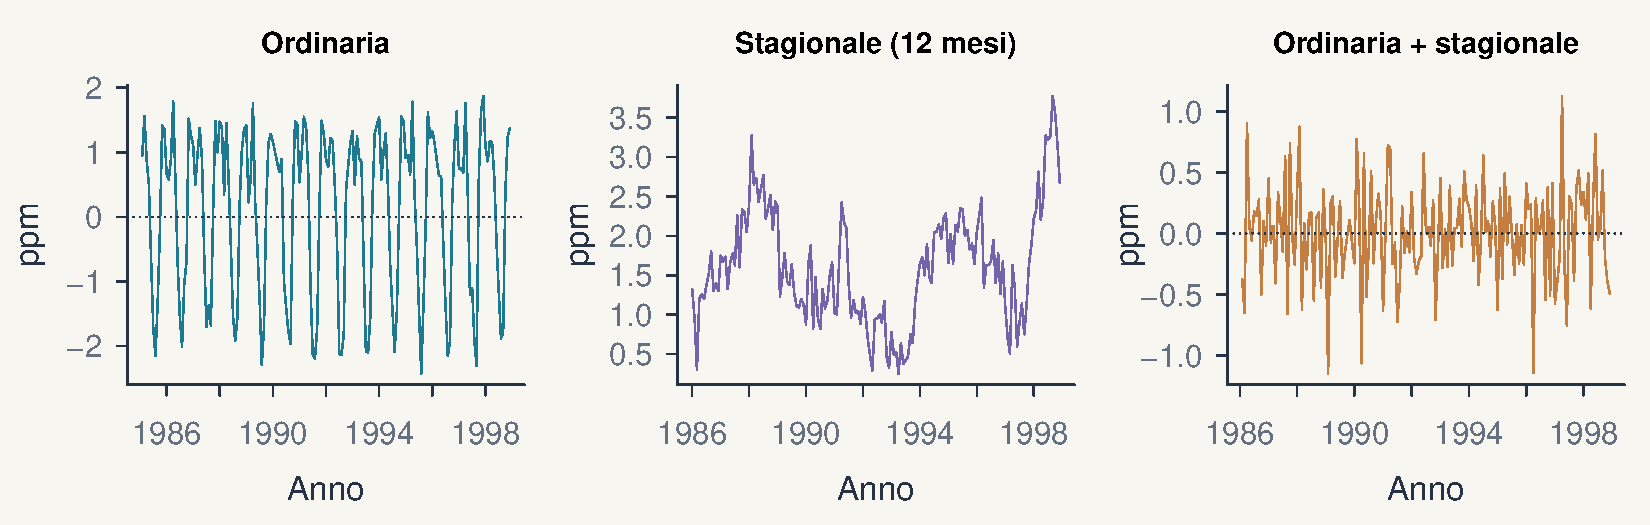
\includegraphics[width=18.05cm,height=5.8cm,keepaspectratio]{Risultati/Figure/21_differenze_CO2.pdf}
\end{minipage}\end{lrbox}
\typeout{FULLBOX:044:FullWideBox:\the\ht\FullWideBox:\the\dp\FullWideBox}

\begin{lrbox}{\PilotRightBox}
\begin{minipage}[t]{18.1cm}\raggedright\color{Ink}\fontsize{11.3}{14.8}\selectfont
\PBody{Tre differenze sui soli 168 mesi di train. Il confronto motiva la trasformazione e non dimostra da solo stazionarietà. Ogni differenza cambia la variabile analizzata.}
\end{minipage}\end{lrbox}
\typeout{FULLBOX:044:PilotRightBox:\the\ht\PilotRightBox:\the\dp\PilotRightBox}

\begin{tikzpicture}[remember picture,overlay]
\PilotChrome{Il confronto delle trasformazioni resta nel train}{IV · ARIMA E STAGIONE}{44}{Ogni trasformazione si giustifica attraverso il problema e si valuta senza usare il test finale.}
\node[anchor=north west,inner sep=0] at([xshift=.96cm,yshift=-2.13cm]current page.north west){\usebox{\FullWideBox}};
\node[anchor=north west,inner sep=0] at([xshift=.96cm,yshift=-8.25cm]current page.north west){\usebox{\PilotRightBox}};
\end{tikzpicture}\end{frame}

\begin{frame}[plain]\hypertarget{slide45}{}
\bookmark[level=1,page=45]{La sigla stagionale mantiene distinti sei ordini}
\begin{lrbox}{\TitleBox}
\begin{minipage}[t]{17.7cm}\raggedright\color{Ink}\fontsize{11.3}{14.8}\selectfont
\color{Navy}\bfseries\fontsize{20.6}{24.5}\selectfont La sigla stagionale mantiene distinti sei ordini
\end{minipage}\end{lrbox}
\typeout{FULLBOX:045:TitleBox:\the\ht\TitleBox:\the\dp\TitleBox}

\begin{lrbox}{\RecallBox}
\begin{minipage}[t]{14.3cm}\raggedright\color{Ink}\fontsize{11.3}{14.8}\selectfont
\fontsize{10.3}{13.8}\selectfont Ordini ordinari, ordini stagionali e periodo del ciclo devono restare leggibili nella specifica.
\end{minipage}\end{lrbox}
\typeout{FULLBOX:045:RecallBox:\the\ht\RecallBox:\the\dp\RecallBox}

\begin{lrbox}{\PilotLeftBox}
\begin{minipage}[t]{10.05cm}\raggedright\color{Ink}\fontsize{11.3}{14.8}\selectfont
\[\operatorname{SARIMA}(p,d,q)(P,D,Q)_{12}\]
{\fontsize{10.2}{13.1}\selectfont\renewcommand{\arraystretch}{1.45}\begin{tabular}{@{}p{2.4cm}p{6.7cm}@{}}\toprule
\textbf{Parte} & \textbf{Significato}\\\midrule
$p,d,q$ & AR, differenze, MA ai ritardi ordinari\\
$P,D,Q$ & AR, differenze, MA ai ritardi stagionali\\
12 & Numero di osservazioni in un ciclo annuale\\
\bottomrule\end{tabular}}

\end{minipage}\end{lrbox}
\typeout{FULLBOX:045:PilotLeftBox:\the\ht\PilotLeftBox:\the\dp\PilotLeftBox}

\begin{lrbox}{\PilotRightBox}
\begin{minipage}[t]{7.55cm}\raggedright\color{Ink}\fontsize{11.3}{14.8}\selectfont
\PBody{Gli ordini maiuscoli descrivono la struttura stagionale. Il periodo 12 riguarda dati mensili con ciclo annuale; non è un numero universale.}
\vspace{2.5mm}
\PInfo{Per dati trimestrali il ciclo annuale ha periodo 4. Una frequenza dichiarata male cambia l’interpretazione dei ritardi.}
\PCode{R · descrivere il modello}{045_esempio.R}
\end{minipage}\end{lrbox}
\typeout{FULLBOX:045:PilotRightBox:\the\ht\PilotRightBox:\the\dp\PilotRightBox}

\begin{tikzpicture}[remember picture,overlay]
\PilotChrome{La sigla stagionale mantiene distinti sei ordini}{IV · ARIMA E STAGIONE}{45}{Ordini ordinari, ordini stagionali e periodo del ciclo devono restare leggibili nella specifica.}
\node[anchor=north west,inner sep=0] at([xshift=.96cm,yshift=-2.13cm]current page.north west){\usebox{\PilotLeftBox}};
\node[anchor=north west,inner sep=0] at([xshift=11.52cm,yshift=-2.13cm]current page.north west){\usebox{\PilotRightBox}};
\end{tikzpicture}\end{frame}

\begin{frame}[plain]\hypertarget{slide46}{}
\bookmark[level=1,page=46]{Il modello del laboratorio è prefissato}
\begin{lrbox}{\TitleBox}
\begin{minipage}[t]{17.7cm}\raggedright\color{Ink}\fontsize{11.3}{14.8}\selectfont
\color{Navy}\bfseries\fontsize{20.6}{24.5}\selectfont Il modello del laboratorio è prefissato
\end{minipage}\end{lrbox}
\typeout{FULLBOX:046:TitleBox:\the\ht\TitleBox:\the\dp\TitleBox}

\begin{lrbox}{\RecallBox}
\begin{minipage}[t]{14.3cm}\raggedright\color{Ink}\fontsize{11.3}{14.8}\selectfont
\fontsize{10.3}{13.8}\selectfont La specifica del modello deve precedere la lettura del suo errore finale.
\end{minipage}\end{lrbox}
\typeout{FULLBOX:046:RecallBox:\the\ht\RecallBox:\the\dp\RecallBox}

\begin{lrbox}{\PilotLeftBox}
\begin{minipage}[t]{10.05cm}\raggedright\color{Ink}\fontsize{11.3}{14.8}\selectfont
\[\operatorname{SARIMA}(0,1,1)(0,1,1)_{12}\]
\[(1-B)(1-B^{12})Y_t\]
\[=(1+\theta B)(1+\Theta B^{12})\varepsilon_t\]
\PInfo{Una differenza ordinaria, una differenza stagionale, una componente MA ordinaria e una MA stagionale; nessuna deriva esplicita.}

\end{minipage}\end{lrbox}
\typeout{FULLBOX:046:PilotLeftBox:\the\ht\PilotLeftBox:\the\dp\PilotLeftBox}

\begin{lrbox}{\PilotRightBox}
\begin{minipage}[t]{7.55cm}\raggedright\color{Ink}\fontsize{11.3}{14.8}\selectfont
\PBody{La specifica riprende il laboratorio del sito. Viene stimata sui livelli del train, lasciando a stats::arima il compito di applicare le differenze.}
\vspace{2.5mm}
\PBody{La crescita futura può emergere dall’integrazione e dallo stato stimato. “Senza deriva esplicita” non significa previsione piatta.}
\vspace{2.5mm}

\end{minipage}\end{lrbox}
\typeout{FULLBOX:046:PilotRightBox:\the\ht\PilotRightBox:\the\dp\PilotRightBox}

\begin{tikzpicture}[remember picture,overlay]
\PilotChrome{Il modello del laboratorio è prefissato}{IV · ARIMA E STAGIONE}{46}{La specifica del modello deve precedere la lettura del suo errore finale.}
\node[anchor=north west,inner sep=0] at([xshift=.96cm,yshift=-2.13cm]current page.north west){\usebox{\PilotLeftBox}};
\node[anchor=north west,inner sep=0] at([xshift=11.52cm,yshift=-2.13cm]current page.north west){\usebox{\PilotRightBox}};
\node[anchor=north east,inner sep=0] at([xshift=17.65cm,yshift=-12.06cm]current page.north west){\color{Classical}\fontsize{7.7}{9.2}\selectfont\href{../../03_Notebook_svolti/M10_Futura/M10_N03.html}{M10\_N03 · notebook svolto}};
\end{tikzpicture}\end{frame}

\begin{frame}[plain]\hypertarget{slide47}{}
\bookmark[level=1,page=47]{Il prodotto stagionale introduce anche il ritardo 13}
\begin{lrbox}{\TitleBox}
\begin{minipage}[t]{17.7cm}\raggedright\color{Ink}\fontsize{11.3}{14.8}\selectfont
\color{Navy}\bfseries\fontsize{20.6}{24.5}\selectfont Il prodotto stagionale introduce anche il ritardo 13
\end{minipage}\end{lrbox}
\typeout{FULLBOX:047:TitleBox:\the\ht\TitleBox:\the\dp\TitleBox}

\begin{lrbox}{\RecallBox}
\begin{minipage}[t]{14.3cm}\raggedright\color{Ink}\fontsize{11.3}{14.8}\selectfont
\fontsize{10.3}{13.8}\selectfont Una struttura stagionale moltiplicativa vincola i coefficienti e conserva parsimonia.
\end{minipage}\end{lrbox}
\typeout{FULLBOX:047:RecallBox:\the\ht\RecallBox:\the\dp\RecallBox}

\begin{lrbox}{\PilotLeftBox}
\begin{minipage}[t]{10.05cm}\raggedright\color{Ink}\fontsize{11.3}{14.8}\selectfont
\[(1+\theta B)(1+\Theta B^{12})\]
\[=1+\theta B+\Theta B^{12}+\theta\Theta B^{13}\]
{\fontsize{10.2}{13.1}\selectfont\renewcommand{\arraystretch}{1.45}\begin{tabular}{@{}p{6cm}p{3cm}@{}}\toprule
\textbf{Ritardo dell’innovazione} & \textbf{Coefficiente}\\\midrule
0 & $1$\\
1 & $\theta$\\
12 & $\Theta$\\
13 & $\theta\Theta$\\
\bottomrule\end{tabular}}

\end{minipage}\end{lrbox}
\typeout{FULLBOX:047:PilotLeftBox:\the\ht\PilotLeftBox:\the\dp\PilotLeftBox}

\begin{lrbox}{\PilotRightBox}
\begin{minipage}[t]{7.55cm}\raggedright\color{Ink}\fontsize{11.3}{14.8}\selectfont
\PBody{La struttura moltiplicativa non stima quattro coefficienti liberi. Il termine al ritardo 13 è il prodotto delle due componenti MA.}
\vspace{2.5mm}
\PInfo{Espandere la formula evita di confondere il SARIMA con un MA non stagionale di ordine 13 avente tutti i coefficienti liberi.}

\end{minipage}\end{lrbox}
\typeout{FULLBOX:047:PilotRightBox:\the\ht\PilotRightBox:\the\dp\PilotRightBox}

\begin{tikzpicture}[remember picture,overlay]
\PilotChrome{Il prodotto stagionale introduce anche il ritardo 13}{IV · ARIMA E STAGIONE}{47}{Una struttura stagionale moltiplicativa vincola i coefficienti e conserva parsimonia.}
\node[anchor=north west,inner sep=0] at([xshift=.96cm,yshift=-2.13cm]current page.north west){\usebox{\PilotLeftBox}};
\node[anchor=north west,inner sep=0] at([xshift=11.52cm,yshift=-2.13cm]current page.north west){\usebox{\PilotRightBox}};
\end{tikzpicture}\end{frame}

\begin{frame}[plain]\hypertarget{slide48}{}
\bookmark[level=1,page=48]{Passare i livelli evita di differenziare due volte}
\begin{lrbox}{\TitleBox}
\begin{minipage}[t]{17.7cm}\raggedright\color{Ink}\fontsize{11.3}{14.8}\selectfont
\color{Navy}\bfseries\fontsize{20.6}{24.5}\selectfont Passare i livelli evita di differenziare due volte
\end{minipage}\end{lrbox}
\typeout{FULLBOX:048:TitleBox:\the\ht\TitleBox:\the\dp\TitleBox}

\begin{lrbox}{\RecallBox}
\begin{minipage}[t]{14.3cm}\raggedright\color{Ink}\fontsize{11.3}{14.8}\selectfont
\fontsize{10.3}{13.8}\selectfont I passaggi di trasformazione devono apparire una volta sola nel procedimento.
\end{minipage}\end{lrbox}
\typeout{FULLBOX:048:RecallBox:\the\ht\RecallBox:\the\dp\RecallBox}

\begin{lrbox}{\PilotLeftBox}
\begin{minipage}[t]{10.05cm}\raggedright\color{Ink}\fontsize{11.3}{14.8}\selectfont
{\fontsize{10.2}{13.1}\selectfont\renewcommand{\arraystretch}{1.45}\begin{tabular}{@{}p{4.6cm}p{4.5cm}@{}}\toprule
\textbf{Ingresso alla stima} & \textbf{Ordini coerenti}\\\midrule
Livelli $Y_t$ & $d=1$, $D=1$ nel SARIMA\\
Differenze già calcolate & ARMA della trasformata, senza ripetere $d,D$\\
Livelli e trasformata insieme & Scegliere una sola procedura esplicita\\
\bottomrule\end{tabular}}

\end{minipage}\end{lrbox}
\typeout{FULLBOX:048:PilotLeftBox:\the\ht\PilotLeftBox:\the\dp\PilotLeftBox}

\begin{lrbox}{\PilotRightBox}
\begin{minipage}[t]{7.55cm}\raggedright\color{Ink}\fontsize{11.3}{14.8}\selectfont
\PBody{Nel percorso principale si passa train in livelli. Applicare prima diff e poi mantenere d=1 e D=1 nella chiamata produrrebbe ulteriori differenze.}
\vspace{2.5mm}
\PInfo{La trasformata serve qui all’esplorazione. L’oggetto fit conserva il modello stimato sui livelli per restituire previsioni in ppm.}
\PCode{R · specifica completa sui livelli}{048_esempio.R}
\end{minipage}\end{lrbox}
\typeout{FULLBOX:048:PilotRightBox:\the\ht\PilotRightBox:\the\dp\PilotRightBox}

\begin{tikzpicture}[remember picture,overlay]
\PilotChrome{Passare i livelli evita di differenziare due volte}{IV · ARIMA E STAGIONE}{48}{I passaggi di trasformazione devono apparire una volta sola nel procedimento.}
\node[anchor=north west,inner sep=0] at([xshift=.96cm,yshift=-2.13cm]current page.north west){\usebox{\PilotLeftBox}};
\node[anchor=north west,inner sep=0] at([xshift=11.52cm,yshift=-2.13cm]current page.north west){\usebox{\PilotRightBox}};
\node[anchor=north east,inner sep=0] at([xshift=17.65cm,yshift=-12.06cm]current page.north west){\color{Classical}\fontsize{7.7}{9.2}\selectfont\href{../../03_Notebook_svolti/M10_Futura/M10_N03.html}{M10\_N03 · notebook svolto}};
\end{tikzpicture}\end{frame}

\begin{frame}[plain]\hypertarget{slide49}{}
\bookmark[level=1,page=49]{La verosimiglianza valuta i parametri del modello}
\begin{lrbox}{\TitleBox}
\begin{minipage}[t]{17.7cm}\raggedright\color{Ink}\fontsize{11.3}{14.8}\selectfont
\color{Navy}\bfseries\fontsize{20.6}{24.5}\selectfont La verosimiglianza valuta i parametri del modello
\end{minipage}\end{lrbox}
\typeout{FULLBOX:049:TitleBox:\the\ht\TitleBox:\the\dp\TitleBox}

\begin{lrbox}{\RecallBox}
\begin{minipage}[t]{14.3cm}\raggedright\color{Ink}\fontsize{11.3}{14.8}\selectfont
\fontsize{10.3}{13.8}\selectfont Specificazione statistica e ottimizzazione numerica sono due passaggi da verificare entrambi.
\end{minipage}\end{lrbox}
\typeout{FULLBOX:049:RecallBox:\the\ht\RecallBox:\the\dp\RecallBox}

\begin{lrbox}{\PilotLeftBox}
\begin{minipage}[t]{10.05cm}\raggedright\color{Ink}\fontsize{11.3}{14.8}\selectfont
\[\widehat\vartheta=\arg\max_{\vartheta}\ell(\vartheta;y_{1:T})\]
\begin{tikzpicture}[x=1cm,y=1cm]
\path[use as bounding box](-.1,-.15) rectangle(9.7,4.4);
\node[pFlow,text width=3.3cm,fill=GeoA!7] (a) at(2,3.0){Specifica\\e parametri candidati};
\node[pFlow,text width=3.7cm,fill=GeoB!7] (b) at(7.3,3.0){Verosimiglianza\\dei dati osservati};
\node[pFlow,text width=4.2cm,fill=GeoC!7] (c) at(4.7,0.9){Ottimizzazione numerica};
\draw[pEdge] (a) -- (b);
\draw[pEdge] (b) -- (c);
\draw[pEdge] (c) -- (a);
\end{tikzpicture}

\end{minipage}\end{lrbox}
\typeout{FULLBOX:049:PilotLeftBox:\the\ht\PilotLeftBox:\the\dp\PilotLeftBox}

\begin{lrbox}{\PilotRightBox}
\begin{minipage}[t]{7.55cm}\raggedright\color{Ink}\fontsize{11.3}{14.8}\selectfont
\PBody{La stima ML usa la struttura probabilistica del modello. Per una serie integrata, stats::arima tratta lo stato iniziale attraverso la rappresentazione in spazio di stato.}
\vspace{2.5mm}
\PInfo{Un risultato numerico non basta: si controllano codice di convergenza, coefficienti e matrice di covarianza stimata.}
\PCode{R · leggere la stima}{049_esempio.R}
\end{minipage}\end{lrbox}
\typeout{FULLBOX:049:PilotRightBox:\the\ht\PilotRightBox:\the\dp\PilotRightBox}

\begin{tikzpicture}[remember picture,overlay]
\PilotChrome{La verosimiglianza valuta i parametri del modello}{IV · ARIMA E STAGIONE}{49}{Specificazione statistica e ottimizzazione numerica sono due passaggi da verificare entrambi.}
\node[anchor=north west,inner sep=0] at([xshift=.96cm,yshift=-2.13cm]current page.north west){\usebox{\PilotLeftBox}};
\node[anchor=north west,inner sep=0] at([xshift=11.52cm,yshift=-2.13cm]current page.north west){\usebox{\PilotRightBox}};
\end{tikzpicture}\end{frame}

\begin{frame}[plain]\hypertarget{slide50}{}
\bookmark[level=1,page=50]{I coefficienti stimati restano associati al train}
\begin{lrbox}{\TitleBox}
\begin{minipage}[t]{17.7cm}\raggedright\color{Ink}\fontsize{11.3}{14.8}\selectfont
\color{Navy}\bfseries\fontsize{20.6}{24.5}\selectfont I coefficienti stimati restano associati al train
\end{minipage}\end{lrbox}
\typeout{FULLBOX:050:TitleBox:\the\ht\TitleBox:\the\dp\TitleBox}

\begin{lrbox}{\RecallBox}
\begin{minipage}[t]{14.3cm}\raggedright\color{Ink}\fontsize{11.3}{14.8}\selectfont
\fontsize{10.3}{13.8}\selectfont Interpretare un coefficiente richiede di ricordare quale trasformata e quale convenzione lo definiscono.
\end{minipage}\end{lrbox}
\typeout{FULLBOX:050:RecallBox:\the\ht\RecallBox:\the\dp\RecallBox}

\begin{lrbox}{\PilotLeftBox}
\begin{minipage}[t]{10.05cm}\raggedright\color{Ink}\fontsize{11.3}{14.8}\selectfont
\PLabel{Stima ML sul periodo 1985--1998}
{\fontsize{10.2}{13.1}\selectfont\renewcommand{\arraystretch}{1.45}\begin{tabular}{@{}p{2.9186666666666667cm}p{2.9186666666666667cm}p{2.9186666666666667cm}@{}}\toprule
\textbf{Termine} & \textbf{Stima} & \textbf{Errore standard}\\\midrule
ma1 & -0,329 & 0,078\\
sma1 & -0,890 & 0,115\\
\bottomrule\end{tabular}}
\[\widehat\sigma^2=0,090\ \mathrm{ppm}^2\]

\end{minipage}\end{lrbox}
\typeout{FULLBOX:050:PilotLeftBox:\the\ht\PilotLeftBox:\the\dp\PilotLeftBox}

\begin{lrbox}{\PilotRightBox}
\begin{minipage}[t]{7.55cm}\raggedright\color{Ink}\fontsize{11.3}{14.8}\selectfont
\PBody{Le due componenti MA descrivono dipendenza nella serie differenziata. I coefficienti non misurano direttamente un tasso di crescita annuale della concentrazione.}
\vspace{2.5mm}
\PInfo{Gli errori standard dei coefficienti riassumono l’incertezza di stima sotto il modello. Non sono gli errori standard delle previsioni future.}
\PSmall{Tabelle e formule numeriche sono generate dai risultati R, con arrotondamento soltanto nella presentazione.}

\end{minipage}\end{lrbox}
\typeout{FULLBOX:050:PilotRightBox:\the\ht\PilotRightBox:\the\dp\PilotRightBox}

\begin{tikzpicture}[remember picture,overlay]
\PilotChrome{I coefficienti stimati restano associati al train}{IV · ARIMA E STAGIONE}{50}{Interpretare un coefficiente richiede di ricordare quale trasformata e quale convenzione lo definiscono.}
\node[anchor=north west,inner sep=0] at([xshift=.96cm,yshift=-2.13cm]current page.north west){\usebox{\PilotLeftBox}};
\node[anchor=north west,inner sep=0] at([xshift=11.52cm,yshift=-2.13cm]current page.north west){\usebox{\PilotRightBox}};
\end{tikzpicture}\end{frame}

\begin{frame}[plain]\hypertarget{slide51}{}
\bookmark[level=1,page=51]{Media, intercetta e deriva richiedono attenzione}
\begin{lrbox}{\TitleBox}
\begin{minipage}[t]{17.7cm}\raggedright\color{Ink}\fontsize{11.3}{14.8}\selectfont
\color{Navy}\bfseries\fontsize{20.6}{24.5}\selectfont Media, intercetta e deriva richiedono attenzione
\end{minipage}\end{lrbox}
\typeout{FULLBOX:051:TitleBox:\the\ht\TitleBox:\the\dp\TitleBox}

\begin{lrbox}{\RecallBox}
\begin{minipage}[t]{14.3cm}\raggedright\color{Ink}\fontsize{11.3}{14.8}\selectfont
\fontsize{10.3}{13.8}\selectfont Il nome di un argomento non sostituisce la lettura della parametrizzazione del modello.
\end{minipage}\end{lrbox}
\typeout{FULLBOX:051:RecallBox:\the\ht\RecallBox:\the\dp\RecallBox}

\begin{lrbox}{\PilotLeftBox}
\begin{minipage}[t]{10.05cm}\raggedright\color{Ink}\fontsize{11.3}{14.8}\selectfont
{\fontsize{10.2}{13.1}\selectfont\renewcommand{\arraystretch}{1.45}\begin{tabular}{@{}p{4.2cm}p{4.9cm}@{}}\toprule
\textbf{Caso} & \textbf{Convenzione utilizzata}\\\midrule
ARMA non differenziato & include.mean può stimare una media\\
ARIMA con differenze & include.mean non aggiunge una deriva\\
Deriva esplicita & Richiede una parametrizzazione coerente\\
Modello del laboratorio & Nessun regressore di deriva esplicita\\
\bottomrule\end{tabular}}

\end{minipage}\end{lrbox}
\typeout{FULLBOX:051:PilotLeftBox:\the\ht\PilotLeftBox:\the\dp\PilotLeftBox}

\begin{lrbox}{\PilotRightBox}
\begin{minipage}[t]{7.55cm}\raggedright\color{Ink}\fontsize{11.3}{14.8}\selectfont
\PBody{In stats::arima, include.mean viene ignorato quando sono presenti differenze. Non basta impostarlo a TRUE per ottenere una deriva nel livello.}
\vspace{2.5mm}
\PInfo{Con più ordini di integrazione, aggiungere termini deterministici può implicare andamenti polinomiali. Serve esplicitare quale crescita si sta imponendo.}

\end{minipage}\end{lrbox}
\typeout{FULLBOX:051:PilotRightBox:\the\ht\PilotRightBox:\the\dp\PilotRightBox}

\begin{tikzpicture}[remember picture,overlay]
\PilotChrome{Media, intercetta e deriva richiedono attenzione}{IV · ARIMA E STAGIONE}{51}{Il nome di un argomento non sostituisce la lettura della parametrizzazione del modello.}
\node[anchor=north west,inner sep=0] at([xshift=.96cm,yshift=-2.13cm]current page.north west){\usebox{\PilotLeftBox}};
\node[anchor=north west,inner sep=0] at([xshift=11.52cm,yshift=-2.13cm]current page.north west){\usebox{\PilotRightBox}};
\end{tikzpicture}\end{frame}

\begin{frame}[plain]\hypertarget{slide52}{}
\bookmark[level=1,page=52]{Una famiglia piccola di candidati}
\begin{lrbox}{\TitleBox}
\begin{minipage}[t]{17.7cm}\raggedright\color{Ink}\fontsize{11.3}{14.8}\selectfont
\color{Navy}\bfseries\fontsize{20.6}{24.5}\selectfont Una famiglia piccola di candidati
\end{minipage}\end{lrbox}
\typeout{FULLBOX:052:TitleBox:\the\ht\TitleBox:\the\dp\TitleBox}

\begin{lrbox}{\RecallBox}
\begin{minipage}[t]{14.3cm}\raggedright\color{Ink}\fontsize{11.3}{14.8}\selectfont
\fontsize{10.3}{13.8}\selectfont La famiglia dei candidati deve essere motivata prima di consultare la verifica finale.
\end{minipage}\end{lrbox}
\typeout{FULLBOX:052:RecallBox:\the\ht\RecallBox:\the\dp\RecallBox}

\begin{lrbox}{\PilotLeftBox}
\begin{minipage}[t]{10.05cm}\raggedright\color{Ink}\fontsize{11.3}{14.8}\selectfont
{\fontsize{10.2}{13.1}\selectfont\renewcommand{\arraystretch}{1.45}\begin{tabular}{@{}p{6.6cm}p{2.5cm}@{}}\toprule
\textbf{Candidato} & \textbf{Parte ordinaria}\\\midrule
SARIMA $(0,1,1)(0,1,1)_{12}$ & MA(1)\\
SARIMA $(1,1,0)(0,1,1)_{12}$ & AR(1)\\
SARIMA $(1,1,1)(0,1,1)_{12}$ & ARMA(1,1)\\
\bottomrule\end{tabular}}

\end{minipage}\end{lrbox}
\typeout{FULLBOX:052:PilotLeftBox:\the\ht\PilotLeftBox:\the\dp\PilotLeftBox}

\begin{lrbox}{\PilotRightBox}
\begin{minipage}[t]{7.55cm}\raggedright\color{Ink}\fontsize{11.3}{14.8}\selectfont
\PBody{L’approfondimento confronta tre strutture mantenendo la stessa finestra, le stesse differenze e lo stesso metodo di stima.}
\vspace{2.5mm}
\PInfo{La specifica centrale resta quella prefissata dal sito. Il confronto illustra come documentare una scelta sul train, senza riscrivere il risultato finale dopo aver visto il test.}
\PSmall{Un insieme piccolo e motivato è più leggibile di una ricerca indiscriminata su molte combinazioni.}

\end{minipage}\end{lrbox}
\typeout{FULLBOX:052:PilotRightBox:\the\ht\PilotRightBox:\the\dp\PilotRightBox}

\begin{tikzpicture}[remember picture,overlay]
\PilotChrome{Una famiglia piccola di candidati}{IV · ARIMA E STAGIONE}{52}{La famiglia dei candidati deve essere motivata prima di consultare la verifica finale.}
\node[anchor=north west,inner sep=0] at([xshift=.96cm,yshift=-2.13cm]current page.north west){\usebox{\PilotLeftBox}};
\node[anchor=north west,inner sep=0] at([xshift=11.52cm,yshift=-2.13cm]current page.north west){\usebox{\PilotRightBox}};
\end{tikzpicture}\end{frame}

\begin{frame}[plain]\hypertarget{slide53}{}
\bookmark[level=1,page=53]{AIC e BIC bilanciano adattamento e parametri}
\begin{lrbox}{\TitleBox}
\begin{minipage}[t]{17.7cm}\raggedright\color{Ink}\fontsize{11.3}{14.8}\selectfont
\color{Navy}\bfseries\fontsize{20.6}{24.5}\selectfont AIC e BIC bilanciano adattamento e parametri
\end{minipage}\end{lrbox}
\typeout{FULLBOX:053:TitleBox:\the\ht\TitleBox:\the\dp\TitleBox}

\begin{lrbox}{\RecallBox}
\begin{minipage}[t]{14.3cm}\raggedright\color{Ink}\fontsize{11.3}{14.8}\selectfont
\fontsize{10.3}{13.8}\selectfont Un criterio informativo orienta la scelta sul campione disponibile; non sostituisce la validazione temporale.
\end{minipage}\end{lrbox}
\typeout{FULLBOX:053:RecallBox:\the\ht\RecallBox:\the\dp\RecallBox}

\begin{lrbox}{\PilotLeftBox}
\begin{minipage}[t]{10.05cm}\raggedright\color{Ink}\fontsize{11.3}{14.8}\selectfont
\[\operatorname{AIC}=-2\widehat\ell+2k\]
\[\operatorname{BIC}=-2\widehat\ell+k\log n\]
\PInfo{Qui $k$ include la varianza. Il campione efficace della verosimiglianza ha $n=155$, dopo le 13 posizioni iniziali associate alle differenze.}

\end{minipage}\end{lrbox}
\typeout{FULLBOX:053:PilotLeftBox:\the\ht\PilotLeftBox:\the\dp\PilotLeftBox}

\begin{lrbox}{\PilotRightBox}
\begin{minipage}[t]{7.55cm}\raggedright\color{Ink}\fontsize{11.3}{14.8}\selectfont
\PBody{Questi criteri confrontano modelli con verosimiglianze comparabili. Valori più bassi indicano il compromesso preferito dal criterio, non un errore futuro già misurato.}
\vspace{2.5mm}
\PInfo{Nel confronto usiamo lo stesso train e gli stessi $d,D$. Cambiare differenze o risposta può rendere non confrontabili i valori riportati.}
\PCode{R · criteri sul train}{053_esempio.R}
\end{minipage}\end{lrbox}
\typeout{FULLBOX:053:PilotRightBox:\the\ht\PilotRightBox:\the\dp\PilotRightBox}

\begin{tikzpicture}[remember picture,overlay]
\PilotChrome{AIC e BIC bilanciano adattamento e parametri}{IV · ARIMA E STAGIONE}{53}{Un criterio informativo orienta la scelta sul campione disponibile; non sostituisce la validazione temporale.}
\node[anchor=north west,inner sep=0] at([xshift=.96cm,yshift=-2.13cm]current page.north west){\usebox{\PilotLeftBox}};
\node[anchor=north west,inner sep=0] at([xshift=11.52cm,yshift=-2.13cm]current page.north west){\usebox{\PilotRightBox}};
\end{tikzpicture}\end{frame}

\begin{frame}[plain]\hypertarget{slide54}{}
\bookmark[level=1,page=54]{Leggere il confronto entro le sue condizioni}
\begin{lrbox}{\TitleBox}
\begin{minipage}[t]{17.7cm}\raggedright\color{Ink}\fontsize{11.3}{14.8}\selectfont
\color{Navy}\bfseries\fontsize{20.6}{24.5}\selectfont Leggere il confronto entro le sue condizioni
\end{minipage}\end{lrbox}
\typeout{FULLBOX:054:TitleBox:\the\ht\TitleBox:\the\dp\TitleBox}

\begin{lrbox}{\RecallBox}
\begin{minipage}[t]{14.3cm}\raggedright\color{Ink}\fontsize{11.3}{14.8}\selectfont
\fontsize{10.3}{13.8}\selectfont Un minimo in una piccola tabella non dimostra che il modello sia universalmente migliore.
\end{minipage}\end{lrbox}
\typeout{FULLBOX:054:RecallBox:\the\ht\RecallBox:\the\dp\RecallBox}

\begin{lrbox}{\PilotLeftBox}
\begin{minipage}[t]{10.05cm}\raggedright\color{Ink}\fontsize{11.3}{14.8}\selectfont
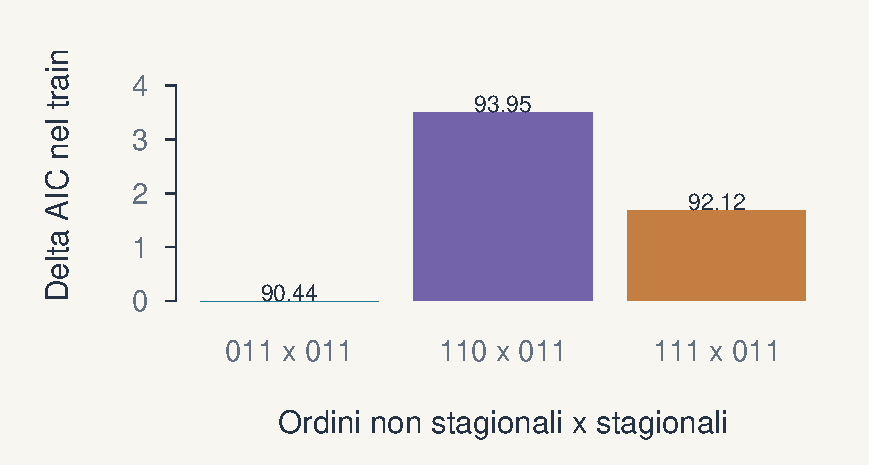
\includegraphics[width=9.85cm,height=5.25cm,keepaspectratio]{Risultati/Figure/22_AIC_train.pdf}
\vspace{1.5mm}
\PSmall{Tre specifiche sullo stesso train e con le stesse differenze. Altezze: $\Delta$AIC; numeri: AIC assoluto.}

\end{minipage}\end{lrbox}
\typeout{FULLBOX:054:PilotLeftBox:\the\ht\PilotLeftBox:\the\dp\PilotLeftBox}

\begin{lrbox}{\PilotRightBox}
\begin{minipage}[t]{7.55cm}\raggedright\color{Ink}\fontsize{11.3}{14.8}\selectfont
\PBody{La graduatoria riguarda soltanto i candidati considerati. Un valore vicino fra modelli suggerisce prudenza nel trattare la scelta come definitiva.}
\vspace{2.5mm}
\PInfo{Convergenza, diagnostica, semplicità e prestazione interna restano elementi distinti da riportare.}
\PBody{Il modello centrale conserva la specifica del laboratorio, così i risultati sono confrontabili con il sito.}
\vspace{2.5mm}

\end{minipage}\end{lrbox}
\typeout{FULLBOX:054:PilotRightBox:\the\ht\PilotRightBox:\the\dp\PilotRightBox}

\begin{tikzpicture}[remember picture,overlay]
\PilotChrome{Leggere il confronto entro le sue condizioni}{IV · ARIMA E STAGIONE}{54}{Un minimo in una piccola tabella non dimostra che il modello sia universalmente migliore.}
\node[anchor=north west,inner sep=0] at([xshift=.96cm,yshift=-2.13cm]current page.north west){\usebox{\PilotLeftBox}};
\node[anchor=north west,inner sep=0] at([xshift=11.52cm,yshift=-2.13cm]current page.north west){\usebox{\PilotRightBox}};
\end{tikzpicture}\end{frame}

\begin{frame}[plain]\hypertarget{slide55}{}
\bookmark[level=1,page=55]{La previsione torna nella scala dei livelli}
\begin{lrbox}{\TitleBox}
\begin{minipage}[t]{17.7cm}\raggedright\color{Ink}\fontsize{11.3}{14.8}\selectfont
\color{Navy}\bfseries\fontsize{20.6}{24.5}\selectfont La previsione torna nella scala dei livelli
\end{minipage}\end{lrbox}
\typeout{FULLBOX:055:TitleBox:\the\ht\TitleBox:\the\dp\TitleBox}

\begin{lrbox}{\RecallBox}
\begin{minipage}[t]{14.3cm}\raggedright\color{Ink}\fontsize{11.3}{14.8}\selectfont
\fontsize{10.3}{13.8}\selectfont La scala della previsione deve coincidere con quella del valore futuro valutato.
\end{minipage}\end{lrbox}
\typeout{FULLBOX:055:RecallBox:\the\ht\RecallBox:\the\dp\RecallBox}

\begin{lrbox}{\PilotLeftBox}
\begin{minipage}[t]{10.05cm}\raggedright\color{Ink}\fontsize{11.3}{14.8}\selectfont
\begin{tikzpicture}[x=1cm,y=1cm]
\path[use as bounding box](-.1,-.15) rectangle(9.7,4.8);
\node[pFlow,text width=3.3cm,fill=GeoA!7] (a) at(2.0,3.4){Modello stimato\\sui livelli del train};
\node[pFlow,text width=3.7cm,fill=GeoB!7] (b) at(7.2,3.4){Previsione\\e varianza a ogni $h$};
\node[pFlow,text width=5.4cm,fill=GeoC!7] (c) at(4.6,1.0){Date future e unità in ppm};
\draw[pEdge] (a) -- (b);
\draw[pEdge] (b) -- (c);
\end{tikzpicture}
\[\widehat y_{T+h\mid T},\qquad s_h=\sqrt{\widehat{\operatorname{Var}}(e_h)}\]

\end{minipage}\end{lrbox}
\typeout{FULLBOX:055:PilotLeftBox:\the\ht\PilotLeftBox:\the\dp\PilotLeftBox}

\begin{lrbox}{\PilotRightBox}
\begin{minipage}[t]{7.55cm}\raggedright\color{Ink}\fontsize{11.3}{14.8}\selectfont
\PBody{predict applicato all’oggetto arima restituisce il centro e l’errore standard dei valori futuri. Non occorre sommare manualmente le differenze quando il modello è stato stimato sui livelli.}
\vspace{2.5mm}
\PInfo{Le date vanno assegnate e controllate esplicitamente prima di confrontare previsione e osservazione.}
\PCode{R · previsione e errore standard}{055_esempio.R}
\end{minipage}\end{lrbox}
\typeout{FULLBOX:055:PilotRightBox:\the\ht\PilotRightBox:\the\dp\PilotRightBox}

\begin{tikzpicture}[remember picture,overlay]
\PilotChrome{La previsione torna nella scala dei livelli}{IV · ARIMA E STAGIONE}{55}{La scala della previsione deve coincidere con quella del valore futuro valutato.}
\node[anchor=north west,inner sep=0] at([xshift=.96cm,yshift=-2.13cm]current page.north west){\usebox{\PilotLeftBox}};
\node[anchor=north west,inner sep=0] at([xshift=11.52cm,yshift=-2.13cm]current page.north west){\usebox{\PilotRightBox}};
\node[anchor=north east,inner sep=0] at([xshift=17.65cm,yshift=-12.06cm]current page.north west){\color{Classical}\fontsize{7.7}{9.2}\selectfont\href{../../03_Notebook_svolti/M10_Futura/M10_N06.html}{M10\_N06 · notebook svolto}};
\end{tikzpicture}\end{frame}

\begin{frame}[plain]\hypertarget{slide56}{}
\bookmark[level=1,page=56]{Un random walk accumula incertezza senza limite}
\begin{lrbox}{\TitleBox}
\begin{minipage}[t]{17.7cm}\raggedright\color{Ink}\fontsize{11.3}{14.8}\selectfont
\color{Navy}\bfseries\fontsize{20.6}{24.5}\selectfont Un random walk accumula incertezza senza limite
\end{minipage}\end{lrbox}
\typeout{FULLBOX:056:TitleBox:\the\ht\TitleBox:\the\dp\TitleBox}

\begin{lrbox}{\RecallBox}
\begin{minipage}[t]{14.3cm}\raggedright\color{Ink}\fontsize{11.3}{14.8}\selectfont
\fontsize{10.3}{13.8}\selectfont Le radici unitarie cambiano la propagazione degli shock e l’incertezza a orizzonti lunghi.
\end{minipage}\end{lrbox}
\typeout{FULLBOX:056:RecallBox:\the\ht\RecallBox:\the\dp\RecallBox}

\begin{lrbox}{\PilotLeftBox}
\begin{minipage}[t]{10.05cm}\raggedright\color{Ink}\fontsize{11.3}{14.8}\selectfont
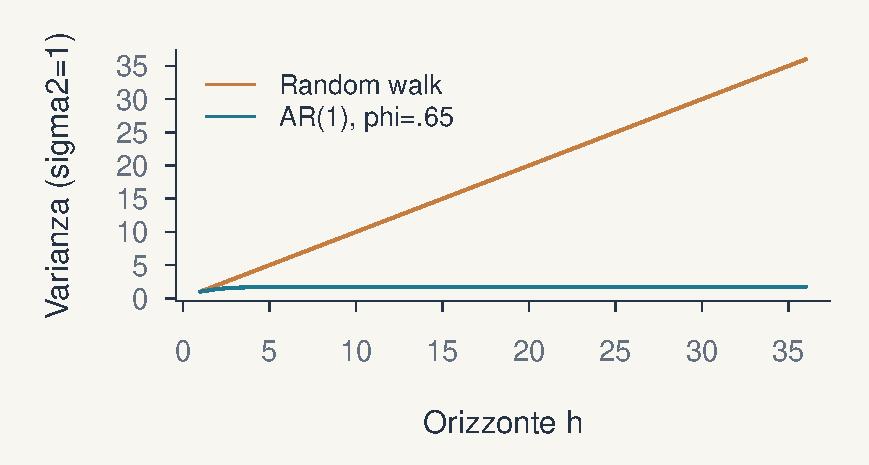
\includegraphics[width=9.85cm,height=5.25cm,keepaspectratio]{Risultati/Figure/25_random_walk_varianza.pdf}
\vspace{1.5mm}
\PSmall{Confronto teorico con parametri noti e innovazioni di varianza unitaria.}
\[Y_t=Y_{t-1}+\varepsilon_t,\qquad\operatorname{Var}(e_h)=h\sigma^2\]

\end{minipage}\end{lrbox}
\typeout{FULLBOX:056:PilotLeftBox:\the\ht\PilotLeftBox:\the\dp\PilotLeftBox}

\begin{lrbox}{\PilotRightBox}
\begin{minipage}[t]{7.55cm}\raggedright\color{Ink}\fontsize{11.3}{14.8}\selectfont
\PBody{Nel random walk ogni innovazione futura entra con peso uno. La varianza dell’errore cresce linearmente con l’orizzonte.}
\vspace{2.5mm}
\PInfo{Il confronto con AR(1) mostra perché la presenza di una radice unitaria cambia il comportamento della previsione di lungo periodo.}
\PSmall{Un SARIMA integrato può avere una crescita dell’incertezza più articolata, legata anche alla stagione.}

\end{minipage}\end{lrbox}
\typeout{FULLBOX:056:PilotRightBox:\the\ht\PilotRightBox:\the\dp\PilotRightBox}

\begin{tikzpicture}[remember picture,overlay]
\PilotChrome{Un random walk accumula incertezza senza limite}{IV · ARIMA E STAGIONE}{56}{Le radici unitarie cambiano la propagazione degli shock e l’incertezza a orizzonti lunghi.}
\node[anchor=north west,inner sep=0] at([xshift=.96cm,yshift=-2.13cm]current page.north west){\usebox{\PilotLeftBox}};
\node[anchor=north west,inner sep=0] at([xshift=11.52cm,yshift=-2.13cm]current page.north west){\usebox{\PilotRightBox}};
\end{tikzpicture}\end{frame}

\begin{frame}[plain]\hypertarget{slide57}{}
\bookmark[level=1,page=57]{Laboratorio: modello e specifica insieme}
\begin{lrbox}{\TitleBox}
\begin{minipage}[t]{17.7cm}\raggedright\color{Ink}\fontsize{11.3}{14.8}\selectfont
\color{Navy}\bfseries\fontsize{20.6}{24.5}\selectfont Laboratorio: modello e specifica insieme
\end{minipage}\end{lrbox}
\typeout{FULLBOX:057:TitleBox:\the\ht\TitleBox:\the\dp\TitleBox}

\begin{lrbox}{\RecallBox}
\begin{minipage}[t]{14.3cm}\raggedright\color{Ink}\fontsize{11.3}{14.8}\selectfont
\fontsize{10.3}{13.8}\selectfont La riproducibilità richiede la procedura completa, oltre all’oggetto finale salvato.
\end{minipage}\end{lrbox}
\typeout{FULLBOX:057:RecallBox:\the\ht\RecallBox:\the\dp\RecallBox}

\begin{lrbox}{\PilotLeftBox}
\begin{minipage}[t]{10.05cm}\raggedright\color{Ink}\fontsize{11.3}{14.8}\selectfont
{\fontsize{10.2}{13.1}\selectfont\renewcommand{\arraystretch}{1.45}\begin{tabular}{@{}p{4.0cm}p{5.1cm}@{}}\toprule
\textbf{Oggetto conservato} & \textbf{Perché serve}\\\midrule
Dati e separazione & Ripetere esattamente la stima\\
Ordini e metodo & Ricostruire la specifica\\
Coefficienti e convergenza & Valutare la soluzione numerica\\
Modello RDS & Riprendere la previsione\\
Versione di R & Interpretare differenze numeriche\\
\bottomrule\end{tabular}}

\end{minipage}\end{lrbox}
\typeout{FULLBOX:057:PilotLeftBox:\the\ht\PilotLeftBox:\the\dp\PilotLeftBox}

\begin{lrbox}{\PilotRightBox}
\begin{minipage}[t]{7.55cm}\raggedright\color{Ink}\fontsize{11.3}{14.8}\selectfont
\PBody{M10\_N03 costruisce il modello; M10\_N09 esporta le previsioni. La consegna conserva sia i numeri leggibili sia gli oggetti necessari alla riproduzione.}
\vspace{2.5mm}
\PInfo{Un oggetto RDS è utile per riprendere il lavoro. Dati e script restano necessari per spiegare da dove proviene.}
\PCode{R · identificare l’oggetto stimato}{057_esempio.R}
\end{minipage}\end{lrbox}
\typeout{FULLBOX:057:PilotRightBox:\the\ht\PilotRightBox:\the\dp\PilotRightBox}

\begin{tikzpicture}[remember picture,overlay]
\PilotChrome{Laboratorio: modello e specifica insieme}{IV · ARIMA E STAGIONE}{57}{La riproducibilità richiede la procedura completa, oltre all’oggetto finale salvato.}
\node[anchor=north west,inner sep=0] at([xshift=.96cm,yshift=-2.13cm]current page.north west){\usebox{\PilotLeftBox}};
\node[anchor=north west,inner sep=0] at([xshift=11.52cm,yshift=-2.13cm]current page.north west){\usebox{\PilotRightBox}};
\node[anchor=north east,inner sep=0] at([xshift=17.65cm,yshift=-12.06cm]current page.north west){\color{Classical}\fontsize{7.7}{9.2}\selectfont\href{../../03_Notebook_svolti/M10_Futura/M10_N09.html}{M10\_N09 · notebook svolto}};
\end{tikzpicture}\end{frame}

\begin{frame}[plain]\hypertarget{slide58}{}
\bookmark[level=0,page=58]{V · DIAGNOSTICA}
\bookmark[level=1,page=58]{La diagnostica esamina ciò che il modello lascia}
\begin{lrbox}{\TitleBox}
\begin{minipage}[t]{17.7cm}\raggedright\color{Ink}\fontsize{11.3}{14.8}\selectfont
\color{Navy}\bfseries\fontsize{20.6}{24.5}\selectfont La diagnostica esamina ciò che il modello lascia
\end{minipage}\end{lrbox}
\typeout{FULLBOX:058:TitleBox:\the\ht\TitleBox:\the\dp\TitleBox}

\begin{lrbox}{\RecallBox}
\begin{minipage}[t]{14.3cm}\raggedright\color{Ink}\fontsize{11.3}{14.8}\selectfont
\fontsize{10.3}{13.8}\selectfont La diagnostica cerca informazione rimasta nei residui, senza trasformarsi in una prova di perfezione.
\end{minipage}\end{lrbox}
\typeout{FULLBOX:058:RecallBox:\the\ht\RecallBox:\the\dp\RecallBox}

\begin{lrbox}{\PilotLeftBox}
\begin{minipage}[t]{10.05cm}\raggedright\color{Ink}\fontsize{11.3}{14.8}\selectfont
\begin{tikzpicture}[x=1cm,y=1cm]
\path[use as bounding box](-.1,-.15) rectangle(9.7,4.8);
\node[pFlow,text width=3.2cm,fill=GeoA!7] (a) at(2.0,3.5){Serie osservata};
\node[pFlow,text width=3.5cm,fill=GeoB!7] (b) at(7.1,3.5){Modello stimato};
\node[pFlow,text width=3.2cm,fill=GeoC!7] (c) at(2.0,1.1){Innovazioni stimate};
\node[pFlow,text width=3.5cm,fill=GeoB!7] (d) at(7.1,1.1){Strutture residue?};
\draw[pEdge] (a) -- (b);
\draw[pEdge] (b) -- (c);
\draw[pEdge] (c) -- (d);
\end{tikzpicture}

\end{minipage}\end{lrbox}
\typeout{FULLBOX:058:PilotLeftBox:\the\ht\PilotLeftBox:\the\dp\PilotLeftBox}

\begin{lrbox}{\PilotRightBox}
\begin{minipage}[t]{7.55cm}\raggedright\color{Ink}\fontsize{11.3}{14.8}\selectfont
\PBody{Le innovazioni stimate dovrebbero essere compatibili con la struttura assunta. Sequenze, dipendenze e cambiamenti di dispersione indicano aspetti da approfondire.}
\vspace{2.5mm}
\PInfo{Un residuo non è un’innovazione teorica osservata direttamente. Deriva dalla stima e dall’inizializzazione del modello.}
\PBody{La diagnostica usa il train. Il test finale rimane disponibile per misurare la prestazione della procedura fissata.}
\vspace{2.5mm}

\end{minipage}\end{lrbox}
\typeout{FULLBOX:058:PilotRightBox:\the\ht\PilotRightBox:\the\dp\PilotRightBox}

\begin{tikzpicture}[remember picture,overlay]
\PilotChrome{La diagnostica esamina ciò che il modello lascia}{V · DIAGNOSTICA}{58}{La diagnostica cerca informazione rimasta nei residui, senza trasformarsi in una prova di perfezione.}
\node[anchor=north west,inner sep=0] at([xshift=.96cm,yshift=-2.13cm]current page.north west){\usebox{\PilotLeftBox}};
\node[anchor=north west,inner sep=0] at([xshift=11.52cm,yshift=-2.13cm]current page.north west){\usebox{\PilotRightBox}};
\node[anchor=north east,inner sep=0] at([xshift=17.65cm,yshift=-12.06cm]current page.north west){\color{Classical}\fontsize{7.7}{9.2}\selectfont\href{../../03_Notebook_svolti/M10_Futura/M10_N04.html}{M10\_N04 · notebook svolto}};
\end{tikzpicture}\end{frame}

\begin{frame}[plain]\hypertarget{slide59}{}
\bookmark[level=1,page=59]{I primi residui risentono dell’inizializzazione}
\begin{lrbox}{\TitleBox}
\begin{minipage}[t]{17.7cm}\raggedright\color{Ink}\fontsize{11.3}{14.8}\selectfont
\color{Navy}\bfseries\fontsize{20.6}{24.5}\selectfont I primi residui risentono dell’inizializzazione
\end{minipage}\end{lrbox}
\typeout{FULLBOX:059:TitleBox:\the\ht\TitleBox:\the\dp\TitleBox}

\begin{lrbox}{\RecallBox}
\begin{minipage}[t]{14.3cm}\raggedright\color{Ink}\fontsize{11.3}{14.8}\selectfont
\fontsize{10.3}{13.8}\selectfont Una scelta sui residui iniziali deve essere documentata e applicata prima dei test.
\end{minipage}\end{lrbox}
\typeout{FULLBOX:059:RecallBox:\the\ht\RecallBox:\the\dp\RecallBox}

\begin{lrbox}{\PilotLeftBox}
\begin{minipage}[t]{10.05cm}\raggedright\color{Ink}\fontsize{11.3}{14.8}\selectfont
\[r_t=\widehat\varepsilon_t,\qquad t=14,\ldots,168\]
{\fontsize{10.2}{13.1}\selectfont\renewcommand{\arraystretch}{1.45}\begin{tabular}{@{}p{5.0cm}p{4.0cm}@{}}\toprule
\textbf{Quantità} & \textbf{Valore nel laboratorio}\\\midrule
Residui disponibili nel fit & 168 posizioni\\
Intervallo diagnostico & Dalla posizione 14\\
Residui esaminati & 155 valori finiti\\
Motivazione & Convenzione coerente con l’inizializzazione\\
\bottomrule\end{tabular}}

\end{minipage}\end{lrbox}
\typeout{FULLBOX:059:PilotLeftBox:\the\ht\PilotLeftBox:\the\dp\PilotLeftBox}

\begin{lrbox}{\PilotRightBox}
\begin{minipage}[t]{7.55cm}\raggedright\color{Ink}\fontsize{11.3}{14.8}\selectfont
\PBody{Il percorso online esclude i primi 13 valori dalla diagnostica. Manteniamo questa convenzione e la rendiamo esplicita.}
\vspace{2.5mm}
\PInfo{Non è una regola universale per qualsiasi ARIMA. La quantità da escludere dipende dal modello, dal metodo e dalla valutazione dell’inizializzazione.}
\PCode{R · residui per la diagnostica}{059_esempio.R}
\end{minipage}\end{lrbox}
\typeout{FULLBOX:059:PilotRightBox:\the\ht\PilotRightBox:\the\dp\PilotRightBox}

\begin{tikzpicture}[remember picture,overlay]
\PilotChrome{I primi residui risentono dell’inizializzazione}{V · DIAGNOSTICA}{59}{Una scelta sui residui iniziali deve essere documentata e applicata prima dei test.}
\node[anchor=north west,inner sep=0] at([xshift=.96cm,yshift=-2.13cm]current page.north west){\usebox{\PilotLeftBox}};
\node[anchor=north west,inner sep=0] at([xshift=11.52cm,yshift=-2.13cm]current page.north west){\usebox{\PilotRightBox}};
\node[anchor=north east,inner sep=0] at([xshift=17.65cm,yshift=-12.06cm]current page.north west){\color{Classical}\fontsize{7.7}{9.2}\selectfont\href{../../03_Notebook_svolti/M10_Futura/M10_N04.html}{M10\_N04 · notebook svolto}};
\end{tikzpicture}\end{frame}

\begin{frame}[plain]\hypertarget{slide60}{}
\bookmark[level=1,page=60]{La sequenza residua mantiene il calendario}
\begin{lrbox}{\TitleBox}
\begin{minipage}[t]{17.7cm}\raggedright\color{Ink}\fontsize{11.3}{14.8}\selectfont
\color{Navy}\bfseries\fontsize{20.6}{24.5}\selectfont La sequenza residua mantiene il calendario
\end{minipage}\end{lrbox}
\typeout{FULLBOX:060:TitleBox:\the\ht\TitleBox:\the\dp\TitleBox}

\begin{lrbox}{\RecallBox}
\begin{minipage}[t]{14.3cm}\raggedright\color{Ink}\fontsize{11.3}{14.8}\selectfont
\fontsize{10.3}{13.8}\selectfont Un residuo anomalo va localizzato nel tempo prima di attribuirgli un significato.
\end{minipage}\end{lrbox}
\typeout{FULLBOX:060:RecallBox:\the\ht\RecallBox:\the\dp\RecallBox}

\begin{lrbox}{\PilotLeftBox}
\begin{minipage}[t]{10.05cm}\raggedright\color{Ink}\fontsize{11.3}{14.8}\selectfont
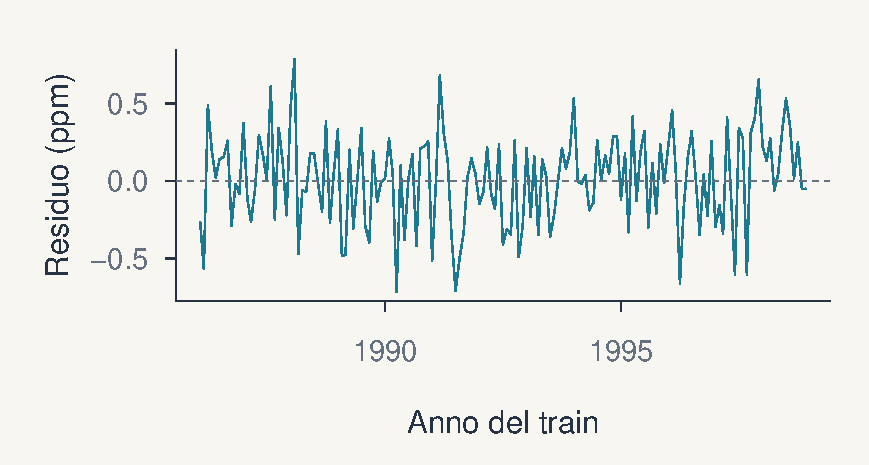
\includegraphics[width=9.85cm,height=5.25cm,keepaspectratio]{Risultati/Figure/08_residui_SARIMA.pdf}
\vspace{1.5mm}
\PSmall{Innovazioni stimate dalla posizione 14; unità in ppm. La linea zero è il riferimento.}

\end{minipage}\end{lrbox}
\typeout{FULLBOX:060:PilotLeftBox:\the\ht\PilotLeftBox:\the\dp\PilotLeftBox}

\begin{lrbox}{\PilotRightBox}
\begin{minipage}[t]{7.55cm}\raggedright\color{Ink}\fontsize{11.3}{14.8}\selectfont
\PBody{Cerchiamo sequenze lunghe dello stesso segno, cambiamenti di dispersione, valori isolati e gruppi di anomalie.}
\vspace{2.5mm}
\PInfo{Un grafico temporale conserva l’ordine. Un istogramma degli stessi residui perderebbe queste informazioni.}
\PBody{La prima lettura è descrittiva: un’anomalia visiva diventa una domanda da verificare, non una spiegazione automatica.}
\vspace{2.5mm}

\end{minipage}\end{lrbox}
\typeout{FULLBOX:060:PilotRightBox:\the\ht\PilotRightBox:\the\dp\PilotRightBox}

\begin{tikzpicture}[remember picture,overlay]
\PilotChrome{La sequenza residua mantiene il calendario}{V · DIAGNOSTICA}{60}{Un residuo anomalo va localizzato nel tempo prima di attribuirgli un significato.}
\node[anchor=north west,inner sep=0] at([xshift=.96cm,yshift=-2.13cm]current page.north west){\usebox{\PilotLeftBox}};
\node[anchor=north west,inner sep=0] at([xshift=11.52cm,yshift=-2.13cm]current page.north west){\usebox{\PilotRightBox}};
\end{tikzpicture}\end{frame}

\begin{frame}[plain]\hypertarget{slide61}{}
\bookmark[level=1,page=61]{Residui centrati possono essere dipendenti}
\begin{lrbox}{\TitleBox}
\begin{minipage}[t]{17.7cm}\raggedright\color{Ink}\fontsize{11.3}{14.8}\selectfont
\color{Navy}\bfseries\fontsize{20.6}{24.5}\selectfont Residui centrati possono essere dipendenti
\end{minipage}\end{lrbox}
\typeout{FULLBOX:061:TitleBox:\the\ht\TitleBox:\the\dp\TitleBox}

\begin{lrbox}{\RecallBox}
\begin{minipage}[t]{14.3cm}\raggedright\color{Ink}\fontsize{11.3}{14.8}\selectfont
\fontsize{10.3}{13.8}\selectfont La diagnostica richiede più di un singolo numero riassuntivo.
\end{minipage}\end{lrbox}
\typeout{FULLBOX:061:RecallBox:\the\ht\RecallBox:\the\dp\RecallBox}

\begin{lrbox}{\PilotLeftBox}
\begin{minipage}[t]{10.05cm}\raggedright\color{Ink}\fontsize{11.3}{14.8}\selectfont
\[\bar r=\frac{1}{n_r}\sum_{t=1}^{n_r}r_t\]
{\fontsize{10.2}{13.1}\selectfont\renewcommand{\arraystretch}{1.45}\begin{tabular}{@{}p{3.2cm}p{5.9cm}@{}}\toprule
\textbf{Controllo} & \textbf{Domanda}\\\midrule
Centro & Resta uno scostamento sistematico?\\
Dispersione & La variabilità è plausibilmente stabile?\\
Ordine & Restano sequenze o cicli?\\
Estremi & Ci sono osservazioni da esaminare?\\
\bottomrule\end{tabular}}

\end{minipage}\end{lrbox}
\typeout{FULLBOX:061:PilotLeftBox:\the\ht\PilotLeftBox:\the\dp\PilotLeftBox}

\begin{lrbox}{\PilotRightBox}
\begin{minipage}[t]{7.55cm}\raggedright\color{Ink}\fontsize{11.3}{14.8}\selectfont
\PBody{Residui mediamente vicini a zero possono essere fortemente correlati. Viceversa, una sequenza senza correlazione evidente può avere una distribuzione problematica per le bande gaussiane.}
\vspace{2.5mm}
\PInfo{Centro, dipendenza e distribuzione vengono controllati con strumenti diversi.}
\PCode{R · riassunti dei residui}{061_esempio.R}
\end{minipage}\end{lrbox}
\typeout{FULLBOX:061:PilotRightBox:\the\ht\PilotRightBox:\the\dp\PilotRightBox}

\begin{tikzpicture}[remember picture,overlay]
\PilotChrome{Residui centrati possono essere dipendenti}{V · DIAGNOSTICA}{61}{La diagnostica richiede più di un singolo numero riassuntivo.}
\node[anchor=north west,inner sep=0] at([xshift=.96cm,yshift=-2.13cm]current page.north west){\usebox{\PilotLeftBox}};
\node[anchor=north west,inner sep=0] at([xshift=11.52cm,yshift=-2.13cm]current page.north west){\usebox{\PilotRightBox}};
\end{tikzpicture}\end{frame}

\begin{frame}[plain]\hypertarget{slide62}{}
\bookmark[level=1,page=62]{L’ACF residua cerca dipendenza lineare rimasta}
\begin{lrbox}{\TitleBox}
\begin{minipage}[t]{17.7cm}\raggedright\color{Ink}\fontsize{11.3}{14.8}\selectfont
\color{Navy}\bfseries\fontsize{20.6}{24.5}\selectfont L’ACF residua cerca dipendenza lineare rimasta
\end{minipage}\end{lrbox}
\typeout{FULLBOX:062:TitleBox:\the\ht\TitleBox:\the\dp\TitleBox}

\begin{lrbox}{\RecallBox}
\begin{minipage}[t]{14.3cm}\raggedright\color{Ink}\fontsize{11.3}{14.8}\selectfont
\fontsize{10.3}{13.8}\selectfont L’ACF residua è una verifica della dipendenza rimasta ai ritardi esaminati.
\end{minipage}\end{lrbox}
\typeout{FULLBOX:062:RecallBox:\the\ht\RecallBox:\the\dp\RecallBox}

\begin{lrbox}{\PilotLeftBox}
\begin{minipage}[t]{10.05cm}\raggedright\color{Ink}\fontsize{11.3}{14.8}\selectfont
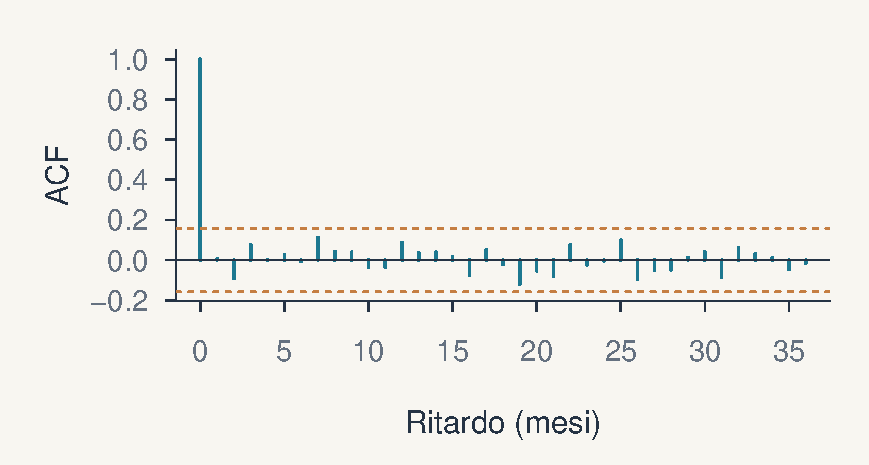
\includegraphics[width=9.85cm,height=5.25cm,keepaspectratio]{Risultati/Figure/09_ACF_residui.pdf}
\vspace{1.5mm}
\PSmall{ACF delle 155 innovazioni stimate. Le bande servono come riferimento approssimato.}

\end{minipage}\end{lrbox}
\typeout{FULLBOX:062:PilotLeftBox:\the\ht\PilotLeftBox:\the\dp\PilotLeftBox}

\begin{lrbox}{\PilotRightBox}
\begin{minipage}[t]{7.55cm}\raggedright\color{Ink}\fontsize{11.3}{14.8}\selectfont
\PBody{Una correlazione residua ai ritardi 12 o 24 suggerirebbe una struttura annuale non completamente rappresentata. Anche i ritardi brevi meritano attenzione.}
\vspace{2.5mm}
\PInfo{Più ritardi si guardano, più è probabile osservare qualche superamento isolato delle bande. Conta la struttura complessiva.}
\PCode{R · ritardi 1, 12 e 24}{062_esempio.R}
\end{minipage}\end{lrbox}
\typeout{FULLBOX:062:PilotRightBox:\the\ht\PilotRightBox:\the\dp\PilotRightBox}

\begin{tikzpicture}[remember picture,overlay]
\PilotChrome{L’ACF residua cerca dipendenza lineare rimasta}{V · DIAGNOSTICA}{62}{L’ACF residua è una verifica della dipendenza rimasta ai ritardi esaminati.}
\node[anchor=north west,inner sep=0] at([xshift=.96cm,yshift=-2.13cm]current page.north west){\usebox{\PilotLeftBox}};
\node[anchor=north west,inner sep=0] at([xshift=11.52cm,yshift=-2.13cm]current page.north west){\usebox{\PilotRightBox}};
\node[anchor=north east,inner sep=0] at([xshift=17.65cm,yshift=-12.06cm]current page.north west){\color{Classical}\fontsize{7.7}{9.2}\selectfont\href{../../03_Notebook_svolti/M10_Futura/M10_N04.html}{M10\_N04 · notebook svolto}};
\end{tikzpicture}\end{frame}

\begin{frame}[plain]\hypertarget{slide63}{}
\bookmark[level=1,page=63]{Le bande dell’ACF non sono un test simultaneo}
\begin{lrbox}{\TitleBox}
\begin{minipage}[t]{17.7cm}\raggedright\color{Ink}\fontsize{11.3}{14.8}\selectfont
\color{Navy}\bfseries\fontsize{20.6}{24.5}\selectfont Le bande dell’ACF non sono un test simultaneo
\end{minipage}\end{lrbox}
\typeout{FULLBOX:063:TitleBox:\the\ht\TitleBox:\the\dp\TitleBox}

\begin{lrbox}{\RecallBox}
\begin{minipage}[t]{14.3cm}\raggedright\color{Ink}\fontsize{11.3}{14.8}\selectfont
\fontsize{10.3}{13.8}\selectfont Una banda grafica puntuale non protegge contemporaneamente tutti i ritardi ispezionati.
\end{minipage}\end{lrbox}
\typeout{FULLBOX:063:RecallBox:\the\ht\RecallBox:\the\dp\RecallBox}

\begin{lrbox}{\PilotLeftBox}
\begin{minipage}[t]{10.05cm}\raggedright\color{Ink}\fontsize{11.3}{14.8}\selectfont
\[\widehat\rho_k\ \approx\ 0\ \pm\ \frac{1{,}96}{\sqrt{n_r}}\]
\PInfo{La formula è un riferimento puntuale approssimato in condizioni di rumore bianco. La stima di parametri e la lettura di molti ritardi complicano l’interpretazione.}

\end{minipage}\end{lrbox}
\typeout{FULLBOX:063:PilotLeftBox:\the\ht\PilotLeftBox:\the\dp\PilotLeftBox}

\begin{lrbox}{\PilotRightBox}
\begin{minipage}[t]{7.55cm}\raggedright\color{Ink}\fontsize{11.3}{14.8}\selectfont
\PBody{Un singolo superamento non basta a dichiarare il modello errato. Una successione coerente di correlazioni può essere più informativa di un picco isolato.}
\vspace{2.5mm}
\PBody{La scelta dei ritardi va collegata alla domanda: breve memoria, ciclo annuale, o dipendenza più lunga.}
\vspace{2.5mm}
\PSmall{Per aggregare più autocorrelazioni useremo Ljung--Box, dichiarando lag e gradi di libertà.}

\end{minipage}\end{lrbox}
\typeout{FULLBOX:063:PilotRightBox:\the\ht\PilotRightBox:\the\dp\PilotRightBox}

\begin{tikzpicture}[remember picture,overlay]
\PilotChrome{Le bande dell’ACF non sono un test simultaneo}{V · DIAGNOSTICA}{63}{Una banda grafica puntuale non protegge contemporaneamente tutti i ritardi ispezionati.}
\node[anchor=north west,inner sep=0] at([xshift=.96cm,yshift=-2.13cm]current page.north west){\usebox{\PilotLeftBox}};
\node[anchor=north west,inner sep=0] at([xshift=11.52cm,yshift=-2.13cm]current page.north west){\usebox{\PilotRightBox}};
\end{tikzpicture}\end{frame}

\begin{frame}[plain]\hypertarget{slide64}{}
\bookmark[level=1,page=64]{Ljung–Box aggrega più correlazioni residue}
\begin{lrbox}{\TitleBox}
\begin{minipage}[t]{17.7cm}\raggedright\color{Ink}\fontsize{11.3}{14.8}\selectfont
\color{Navy}\bfseries\fontsize{20.6}{24.5}\selectfont Ljung–Box aggrega più correlazioni residue
\end{minipage}\end{lrbox}
\typeout{FULLBOX:064:TitleBox:\the\ht\TitleBox:\the\dp\TitleBox}

\begin{lrbox}{\RecallBox}
\begin{minipage}[t]{14.3cm}\raggedright\color{Ink}\fontsize{11.3}{14.8}\selectfont
\fontsize{10.3}{13.8}\selectfont Il risultato di Ljung–Box va riportato insieme a numero di residui, ritardo massimo e correzione.
\end{minipage}\end{lrbox}
\typeout{FULLBOX:064:RecallBox:\the\ht\RecallBox:\the\dp\RecallBox}

\begin{lrbox}{\PilotLeftBox}
\begin{minipage}[t]{10.05cm}\raggedright\color{Ink}\fontsize{11.3}{14.8}\selectfont
\[Q=n_r(n_r+2)\sum_{k=1}^{m}\frac{\widehat\rho_k^2}{n_r-k}\]
\[Q\ \dot\sim\ \chi^2_{m-r},\qquad m=24,\quad r=2\]
\PInfo{Nel protocollo si sottraggono i due coefficienti MA stimati. Restano 22 gradi di libertà per il riferimento asintotico.}

\end{minipage}\end{lrbox}
\typeout{FULLBOX:064:PilotLeftBox:\the\ht\PilotLeftBox:\the\dp\PilotLeftBox}

\begin{lrbox}{\PilotRightBox}
\begin{minipage}[t]{7.55cm}\raggedright\color{Ink}\fontsize{11.3}{14.8}\selectfont
\PBody{L’ipotesi nulla riguarda l’assenza di autocorrelazioni ai ritardi considerati. Il test riassume correlazioni al quadrato e non attribuisce un significato fisico ai loro segni.}
\vspace{2.5mm}
\PBody{Il riferimento è approssimato: dimensione campionaria, stima e modello incidono sulla sua calibrazione.}
\vspace{2.5mm}

\end{minipage}\end{lrbox}
\typeout{FULLBOX:064:PilotRightBox:\the\ht\PilotRightBox:\the\dp\PilotRightBox}

\begin{tikzpicture}[remember picture,overlay]
\PilotChrome{Ljung–Box aggrega più correlazioni residue}{V · DIAGNOSTICA}{64}{Il risultato di Ljung–Box va riportato insieme a numero di residui, ritardo massimo e correzione.}
\node[anchor=north west,inner sep=0] at([xshift=.96cm,yshift=-2.13cm]current page.north west){\usebox{\PilotLeftBox}};
\node[anchor=north west,inner sep=0] at([xshift=11.52cm,yshift=-2.13cm]current page.north west){\usebox{\PilotRightBox}};
\end{tikzpicture}\end{frame}

\begin{frame}[plain]\hypertarget{slide65}{}
\bookmark[level=1,page=65]{Il risultato diagnostico non certifica il modello}
\begin{lrbox}{\TitleBox}
\begin{minipage}[t]{17.7cm}\raggedright\color{Ink}\fontsize{11.3}{14.8}\selectfont
\color{Navy}\bfseries\fontsize{20.6}{24.5}\selectfont Il risultato diagnostico non certifica il modello
\end{minipage}\end{lrbox}
\typeout{FULLBOX:065:TitleBox:\the\ht\TitleBox:\the\dp\TitleBox}

\begin{lrbox}{\RecallBox}
\begin{minipage}[t]{14.3cm}\raggedright\color{Ink}\fontsize{11.3}{14.8}\selectfont
\fontsize{10.3}{13.8}\selectfont La mancata evidenza contro un’ipotesi non è una dimostrazione della sua correttezza.
\end{minipage}\end{lrbox}
\typeout{FULLBOX:065:RecallBox:\the\ht\RecallBox:\the\dp\RecallBox}

\begin{lrbox}{\PilotLeftBox}
\begin{minipage}[t]{10.05cm}\raggedright\color{Ink}\fontsize{11.3}{14.8}\selectfont
\PLabel{Ljung–Box sul protocollo dichiarato}
{\fontsize{10.2}{13.1}\selectfont\renewcommand{\arraystretch}{1.45}\begin{tabular}{@{}p{5.2cm}p{3.8cm}@{}}\toprule
\textbf{Quantità} & \textbf{Risultato}\\\midrule
Residui & 155\\
Ritardo massimo & 24\\
Gradi di libertà & 22\\
Statistica $Q$ & 14,242\\
Valore $p$ & 0,893\\
\bottomrule\end{tabular}}

\end{minipage}\end{lrbox}
\typeout{FULLBOX:065:PilotLeftBox:\the\ht\PilotLeftBox:\the\dp\PilotLeftBox}

\begin{lrbox}{\PilotRightBox}
\begin{minipage}[t]{7.55cm}\raggedright\color{Ink}\fontsize{11.3}{14.8}\selectfont
\PBody{Il valore $p$ quantifica quanto la statistica sia compatibile con il riferimento del test. Non è la probabilità che il modello sia vero.}
\vspace{2.5mm}
\PInfo{Un risultato non significativo non prova indipendenza, normalità o buona previsione. Riguarda questa verifica di autocorrelazione.}
\PCode{R · Ljung–Box}{065_esempio.R}
\end{minipage}\end{lrbox}
\typeout{FULLBOX:065:PilotRightBox:\the\ht\PilotRightBox:\the\dp\PilotRightBox}

\begin{tikzpicture}[remember picture,overlay]
\PilotChrome{Il risultato diagnostico non certifica il modello}{V · DIAGNOSTICA}{65}{La mancata evidenza contro un’ipotesi non è una dimostrazione della sua correttezza.}
\node[anchor=north west,inner sep=0] at([xshift=.96cm,yshift=-2.13cm]current page.north west){\usebox{\PilotLeftBox}};
\node[anchor=north west,inner sep=0] at([xshift=11.52cm,yshift=-2.13cm]current page.north west){\usebox{\PilotRightBox}};
\node[anchor=north east,inner sep=0] at([xshift=17.65cm,yshift=-12.06cm]current page.north west){\color{Classical}\fontsize{7.7}{9.2}\selectfont\href{../../03_Notebook_svolti/M10_Futura/M10_N04.html}{M10\_N04 · notebook svolto}};
\end{tikzpicture}\end{frame}

\begin{frame}[plain]\hypertarget{slide66}{}
\bookmark[level=1,page=66]{Il QQ plot esamina forma e code della distribuzione}
\begin{lrbox}{\TitleBox}
\begin{minipage}[t]{17.7cm}\raggedright\color{Ink}\fontsize{11.3}{14.8}\selectfont
\color{Navy}\bfseries\fontsize{20.6}{24.5}\selectfont Il QQ plot esamina forma e code della distribuzione
\end{minipage}\end{lrbox}
\typeout{FULLBOX:066:TitleBox:\the\ht\TitleBox:\the\dp\TitleBox}

\begin{lrbox}{\RecallBox}
\begin{minipage}[t]{14.3cm}\raggedright\color{Ink}\fontsize{11.3}{14.8}\selectfont
\fontsize{10.3}{13.8}\selectfont La distribuzione dei residui conta soprattutto quando si interpretano probabilità e intervalli.
\end{minipage}\end{lrbox}
\typeout{FULLBOX:066:RecallBox:\the\ht\RecallBox:\the\dp\RecallBox}

\begin{lrbox}{\PilotLeftBox}
\begin{minipage}[t]{10.05cm}\raggedright\color{Ink}\fontsize{11.3}{14.8}\selectfont
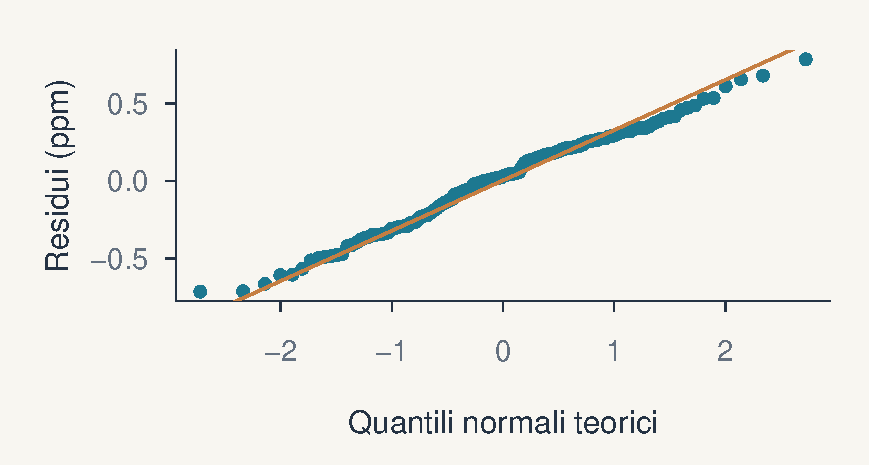
\includegraphics[width=9.85cm,height=5.25cm,keepaspectratio]{Risultati/Figure/10_QQ_residui.pdf}
\vspace{1.5mm}
\PSmall{Quantili campionari delle innovazioni stimate contro quantili gaussiani; linea di riferimento.}

\end{minipage}\end{lrbox}
\typeout{FULLBOX:066:PilotLeftBox:\the\ht\PilotLeftBox:\the\dp\PilotLeftBox}

\begin{lrbox}{\PilotRightBox}
\begin{minipage}[t]{7.55cm}\raggedright\color{Ink}\fontsize{11.3}{14.8}\selectfont
\PBody{Scostamenti nelle code possono rendere meno attendibili intervalli costruiti con una distribuzione normale, anche quando l’ACF residua è modesta.}
\vspace{2.5mm}
\PInfo{Il grafico non dimostra normalità. Permette di localizzare quali parti della distribuzione si allontanano dal riferimento.}
\PSmall{Per prevedere la media non è sempre necessaria la normalità. La probabilità attribuita agli estremi richiede ipotesi più specifiche.}

\end{minipage}\end{lrbox}
\typeout{FULLBOX:066:PilotRightBox:\the\ht\PilotRightBox:\the\dp\PilotRightBox}

\begin{tikzpicture}[remember picture,overlay]
\PilotChrome{Il QQ plot esamina forma e code della distribuzione}{V · DIAGNOSTICA}{66}{La distribuzione dei residui conta soprattutto quando si interpretano probabilità e intervalli.}
\node[anchor=north west,inner sep=0] at([xshift=.96cm,yshift=-2.13cm]current page.north west){\usebox{\PilotLeftBox}};
\node[anchor=north west,inner sep=0] at([xshift=11.52cm,yshift=-2.13cm]current page.north west){\usebox{\PilotRightBox}};
\end{tikzpicture}\end{frame}

\begin{frame}[plain]\hypertarget{slide67}{}
\bookmark[level=1,page=67]{Autocorrelazione e dispersione sono distinte}
\begin{lrbox}{\TitleBox}
\begin{minipage}[t]{17.7cm}\raggedright\color{Ink}\fontsize{11.3}{14.8}\selectfont
\color{Navy}\bfseries\fontsize{20.6}{24.5}\selectfont Autocorrelazione e dispersione sono distinte
\end{minipage}\end{lrbox}
\typeout{FULLBOX:067:TitleBox:\the\ht\TitleBox:\the\dp\TitleBox}

\begin{lrbox}{\RecallBox}
\begin{minipage}[t]{14.3cm}\raggedright\color{Ink}\fontsize{11.3}{14.8}\selectfont
\fontsize{10.3}{13.8}\selectfont Un controllo della media e dell’ACF non esaurisce la verifica della variabilità.
\end{minipage}\end{lrbox}
\typeout{FULLBOX:067:RecallBox:\the\ht\RecallBox:\the\dp\RecallBox}

\begin{lrbox}{\PilotLeftBox}
\begin{minipage}[t]{10.05cm}\raggedright\color{Ink}\fontsize{11.3}{14.8}\selectfont
\[\operatorname{Cov}(\varepsilon_t,\varepsilon_{t-k})=0\]
\[\nRightarrow\quad\operatorname{Var}(\varepsilon_t\mid\mathcal F_{t-1})=\sigma^2\]
\PInfo{Assenza di correlazione lineare e varianza condizionata costante sono proprietà differenti.}

\end{minipage}\end{lrbox}
\typeout{FULLBOX:067:PilotLeftBox:\the\ht\PilotLeftBox:\the\dp\PilotLeftBox}

\begin{lrbox}{\PilotRightBox}
\begin{minipage}[t]{7.55cm}\raggedright\color{Ink}\fontsize{11.3}{14.8}\selectfont
\PBody{Periodi con residui piccoli seguiti da periodi molto dispersi possono segnalare eteroschedasticità. L’ACF dei residui al quadrato è un approfondimento descrittivo.}
\vspace{2.5mm}
\PInfo{In questo modulo non stimiamo una famiglia di modelli di volatilità. Registriamo il limite se la dispersione appare variabile.}
\PCode{R · dipendenza dei quadrati}{067_esempio.R}
\end{minipage}\end{lrbox}
\typeout{FULLBOX:067:PilotRightBox:\the\ht\PilotRightBox:\the\dp\PilotRightBox}

\begin{tikzpicture}[remember picture,overlay]
\PilotChrome{Autocorrelazione e dispersione sono distinte}{V · DIAGNOSTICA}{67}{Un controllo della media e dell’ACF non esaurisce la verifica della variabilità.}
\node[anchor=north west,inner sep=0] at([xshift=.96cm,yshift=-2.13cm]current page.north west){\usebox{\PilotLeftBox}};
\node[anchor=north west,inner sep=0] at([xshift=11.52cm,yshift=-2.13cm]current page.north west){\usebox{\PilotRightBox}};
\end{tikzpicture}\end{frame}

\begin{frame}[plain]\hypertarget{slide68}{}
\bookmark[level=1,page=68]{Documentare l’origine delle anomalie}
\begin{lrbox}{\TitleBox}
\begin{minipage}[t]{17.7cm}\raggedright\color{Ink}\fontsize{11.3}{14.8}\selectfont
\color{Navy}\bfseries\fontsize{20.6}{24.5}\selectfont Documentare l’origine delle anomalie
\end{minipage}\end{lrbox}
\typeout{FULLBOX:068:TitleBox:\the\ht\TitleBox:\the\dp\TitleBox}

\begin{lrbox}{\RecallBox}
\begin{minipage}[t]{14.3cm}\raggedright\color{Ink}\fontsize{11.3}{14.8}\selectfont
\fontsize{10.3}{13.8}\selectfont La pulizia dei dati è una scelta scientifica da motivare, non un modo per migliorare retroattivamente il risultato.
\end{minipage}\end{lrbox}
\typeout{FULLBOX:068:RecallBox:\the\ht\RecallBox:\the\dp\RecallBox}

\begin{lrbox}{\PilotLeftBox}
\begin{minipage}[t]{10.05cm}\raggedright\color{Ink}\fontsize{11.3}{14.8}\selectfont
{\fontsize{10.2}{13.1}\selectfont\renewcommand{\arraystretch}{1.45}\begin{tabular}{@{}p{3.4cm}p{5.7cm}@{}}\toprule
\textbf{Possibile origine} & \textbf{Azione motivata}\\\midrule
Errore di registrazione & Controllare la fonte e conservare la correzione\\
Evento reale & Mantenerlo e discuterne il significato\\
Cambio di procedura & Documentare la discontinuità\\
Modello inadeguato & Rivedere l’ipotesi usando il train\\
\bottomrule\end{tabular}}

\end{minipage}\end{lrbox}
\typeout{FULLBOX:068:PilotLeftBox:\the\ht\PilotLeftBox:\the\dp\PilotLeftBox}

\begin{lrbox}{\PilotRightBox}
\begin{minipage}[t]{7.55cm}\raggedright\color{Ink}\fontsize{11.3}{14.8}\selectfont
\PBody{Eliminare un valore perché peggiora una metrica modifica il problema dopo aver visto il risultato. Le regole di esclusione devono dipendere da una ragione verificabile.}
\vspace{2.5mm}
\PInfo{Se una modifica viene suggerita dal test finale, quel periodo ha partecipato allo sviluppo. Occorre dichiararlo e trovare una nuova verifica indipendente.}

\end{minipage}\end{lrbox}
\typeout{FULLBOX:068:PilotRightBox:\the\ht\PilotRightBox:\the\dp\PilotRightBox}

\begin{tikzpicture}[remember picture,overlay]
\PilotChrome{Documentare l’origine delle anomalie}{V · DIAGNOSTICA}{68}{La pulizia dei dati è una scelta scientifica da motivare, non un modo per migliorare retroattivamente il risultato.}
\node[anchor=north west,inner sep=0] at([xshift=.96cm,yshift=-2.13cm]current page.north west){\usebox{\PilotLeftBox}};
\node[anchor=north west,inner sep=0] at([xshift=11.52cm,yshift=-2.13cm]current page.north west){\usebox{\PilotRightBox}};
\end{tikzpicture}\end{frame}

\begin{frame}[plain]\hypertarget{slide69}{}
\bookmark[level=1,page=69]{Laboratorio: scrivere una conclusione diagnostica}
\begin{lrbox}{\TitleBox}
\begin{minipage}[t]{17.7cm}\raggedright\color{Ink}\fontsize{11.3}{14.8}\selectfont
\color{Navy}\bfseries\fontsize{20.6}{24.5}\selectfont Laboratorio: scrivere una conclusione diagnostica
\end{minipage}\end{lrbox}
\typeout{FULLBOX:069:TitleBox:\the\ht\TitleBox:\the\dp\TitleBox}

\begin{lrbox}{\RecallBox}
\begin{minipage}[t]{14.3cm}\raggedright\color{Ink}\fontsize{11.3}{14.8}\selectfont
\fontsize{10.3}{13.8}\selectfont Una buona conclusione diagnostica nomina sia l’evidenza sia ciò che il controllo non stabilisce.
\end{minipage}\end{lrbox}
\typeout{FULLBOX:069:RecallBox:\the\ht\RecallBox:\the\dp\RecallBox}

\begin{lrbox}{\PilotLeftBox}
\begin{minipage}[t]{10.05cm}\raggedright\color{Ink}\fontsize{11.3}{14.8}\selectfont
\PLabel{Una conclusione in quattro parti}
{\fontsize{10.2}{13.1}\selectfont\renewcommand{\arraystretch}{1.45}\begin{tabular}{@{}p{3.1cm}p{6.0cm}@{}}\toprule
\textbf{Evidenza} & \textbf{Che cosa riportare}\\\midrule
Sequenza & Andamento e anomalie osservate\\
Dipendenza & ACF e lag esaminati\\
Test aggregato & $Q$, gradi di libertà e valore $p$\\
Distribuzione & QQ plot e limiti delle bande\\
\bottomrule\end{tabular}}

\end{minipage}\end{lrbox}
\typeout{FULLBOX:069:PilotLeftBox:\the\ht\PilotLeftBox:\the\dp\PilotLeftBox}

\begin{lrbox}{\PilotRightBox}
\begin{minipage}[t]{7.55cm}\raggedright\color{Ink}\fontsize{11.3}{14.8}\selectfont
\PBody{La conclusione unisce strumenti complementari. Per esempio: “Ai ritardi esaminati non emerge una forte struttura lineare residua; le bande restano condizionate al modello e alle sue ipotesi”.}
\vspace{2.5mm}
\PInfo{M10\_N04 include l’esecuzione e l’interpretazione. La formulazione finale deve seguire i risultati realmente osservati, senza promuovere un test a certificazione generale.}

\end{minipage}\end{lrbox}
\typeout{FULLBOX:069:PilotRightBox:\the\ht\PilotRightBox:\the\dp\PilotRightBox}

\begin{tikzpicture}[remember picture,overlay]
\PilotChrome{Laboratorio: scrivere una conclusione diagnostica}{V · DIAGNOSTICA}{69}{Una buona conclusione diagnostica nomina sia l’evidenza sia ciò che il controllo non stabilisce.}
\node[anchor=north west,inner sep=0] at([xshift=.96cm,yshift=-2.13cm]current page.north west){\usebox{\PilotLeftBox}};
\node[anchor=north west,inner sep=0] at([xshift=11.52cm,yshift=-2.13cm]current page.north west){\usebox{\PilotRightBox}};
\node[anchor=north east,inner sep=0] at([xshift=17.65cm,yshift=-12.06cm]current page.north west){\color{Classical}\fontsize{7.7}{9.2}\selectfont\href{../../03_Notebook_svolti/M10_Futura/M10_N04.html}{M10\_N04 · notebook svolto}};
\end{tikzpicture}\end{frame}

\begin{frame}[plain]\hypertarget{slide70}{}
\bookmark[level=0,page=70]{VI · VALIDAZIONE TEMPORALE}
\bookmark[level=1,page=70]{La validazione rispetta il tempo della decisione}
\begin{lrbox}{\TitleBox}
\begin{minipage}[t]{17.7cm}\raggedright\color{Ink}\fontsize{11.3}{14.8}\selectfont
\color{Navy}\bfseries\fontsize{20.6}{24.5}\selectfont La validazione rispetta il tempo della decisione
\end{minipage}\end{lrbox}
\typeout{FULLBOX:070:TitleBox:\the\ht\TitleBox:\the\dp\TitleBox}

\begin{lrbox}{\RecallBox}
\begin{minipage}[t]{14.3cm}\raggedright\color{Ink}\fontsize{11.3}{14.8}\selectfont
\fontsize{10.3}{13.8}\selectfont Il disegno di validazione deve imitare l’uso previsto del modello.
\end{minipage}\end{lrbox}
\typeout{FULLBOX:070:RecallBox:\the\ht\RecallBox:\the\dp\RecallBox}

\begin{lrbox}{\PilotLeftBox}
\begin{minipage}[t]{10.05cm}\raggedright\color{Ink}\fontsize{11.3}{14.8}\selectfont
\begin{tikzpicture}[x=1cm,y=1cm]
\path[use as bounding box](-.1,-.15) rectangle(9.7,4.9);
\fill[GeoA!20](.5,3.96)rectangle(5.500,4.44);
\fill[GeoB!40](5.500,3.96)rectangle(6.000,4.44);
\node[pNote,anchor=west]at(6.160,4.2){120};
\fill[GeoA!20](.5,3.04)rectangle(6.000,3.5200000000000005);
\fill[GeoB!40](6.000,3.04)rectangle(6.500,3.5200000000000005);
\node[pNote,anchor=west]at(6.660,3.2800000000000002){132};
\fill[GeoA!20](.5,2.12)rectangle(6.500,2.6000000000000005);
\fill[GeoB!40](6.500,2.12)rectangle(7.000,2.6000000000000005);
\node[pNote,anchor=west]at(7.160,2.3600000000000003){144};
\draw[Muted,dashed](7.500,.6)--(7.500,4.65);
\node[pNote]at(4,.25){train in verde · verifica interna in rame};
\node[pNote]at(8.8,4.4){test\\finale};
\end{tikzpicture}
\[\widehat y_{o+h\mid o}=g_h(y_1,\ldots,y_o)\]

\end{minipage}\end{lrbox}
\typeout{FULLBOX:070:PilotLeftBox:\the\ht\PilotLeftBox:\the\dp\PilotLeftBox}

\begin{lrbox}{\PilotRightBox}
\begin{minipage}[t]{7.55cm}\raggedright\color{Ink}\fontsize{11.3}{14.8}\selectfont
\PBody{Ogni previsione interna viene costruita usando soltanto osservazioni antecedenti o contemporanee alla propria origine. Il valore futuro serve dopo, per calcolare l’errore.}
\vspace{2.5mm}
\PInfo{Separare righe a caso può distribuire passato e futuro in entrambe le parti e alterare il compito di previsione temporale.}

\end{minipage}\end{lrbox}
\typeout{FULLBOX:070:PilotRightBox:\the\ht\PilotRightBox:\the\dp\PilotRightBox}

\begin{tikzpicture}[remember picture,overlay]
\PilotChrome{La validazione rispetta il tempo della decisione}{VI · VALIDAZIONE TEMPORALE}{70}{Il disegno di validazione deve imitare l’uso previsto del modello.}
\node[anchor=north west,inner sep=0] at([xshift=.96cm,yshift=-2.13cm]current page.north west){\usebox{\PilotLeftBox}};
\node[anchor=north west,inner sep=0] at([xshift=11.52cm,yshift=-2.13cm]current page.north west){\usebox{\PilotRightBox}};
\node[anchor=north east,inner sep=0] at([xshift=17.65cm,yshift=-12.06cm]current page.north west){\color{Classical}\fontsize{7.7}{9.2}\selectfont\href{../../03_Notebook_svolti/M10_Futura/M10_N05.html}{M10\_N05 · notebook svolto}};
\end{tikzpicture}\end{frame}

\begin{frame}[plain]\hypertarget{slide71}{}
\bookmark[level=1,page=71]{Una finestra crescente conserva tutto il passato}
\begin{lrbox}{\TitleBox}
\begin{minipage}[t]{17.7cm}\raggedright\color{Ink}\fontsize{11.3}{14.8}\selectfont
\color{Navy}\bfseries\fontsize{20.6}{24.5}\selectfont Una finestra crescente conserva tutto il passato
\end{minipage}\end{lrbox}
\typeout{FULLBOX:071:TitleBox:\the\ht\TitleBox:\the\dp\TitleBox}

\begin{lrbox}{\RecallBox}
\begin{minipage}[t]{14.3cm}\raggedright\color{Ink}\fontsize{11.3}{14.8}\selectfont
\fontsize{10.3}{13.8}\selectfont La previsione storica di ogni origine richiede una stima che usi soltanto il suo passato.
\end{minipage}\end{lrbox}
\typeout{FULLBOX:071:RecallBox:\the\ht\RecallBox:\the\dp\RecallBox}

\begin{lrbox}{\PilotLeftBox}
\begin{minipage}[t]{10.05cm}\raggedright\color{Ink}\fontsize{11.3}{14.8}\selectfont
\begin{tikzpicture}[x=1cm,y=1cm]
\path[use as bounding box](-.1,-.15) rectangle(9.7,4.9);
\fill[GeoA!20](.5,3.96)rectangle(5.500,4.44);
\fill[GeoB!40](5.500,3.96)rectangle(6.000,4.44);
\node[pNote,anchor=west]at(6.160,4.2){120};
\fill[GeoA!20](.5,3.04)rectangle(6.000,3.5200000000000005);
\fill[GeoB!40](6.000,3.04)rectangle(6.500,3.5200000000000005);
\node[pNote,anchor=west]at(6.660,3.2800000000000002){132};
\fill[GeoA!20](.5,2.12)rectangle(6.500,2.6000000000000005);
\fill[GeoB!40](6.500,2.12)rectangle(7.000,2.6000000000000005);
\node[pNote,anchor=west]at(7.160,2.3600000000000003){144};
\draw[Muted,dashed](7.500,.6)--(7.500,4.65);
\node[pNote]at(4,.25){train in verde · verifica interna in rame};
\node[pNote]at(8.8,4.4){test\\finale};
\end{tikzpicture}
\PSmall{Origine 120: train 1--120, verifica 121--132.\\Origine 132: train 1--132, verifica 133--144.\\Origine 144: train 1--144, verifica 145--156.}

\end{minipage}\end{lrbox}
\typeout{FULLBOX:071:PilotLeftBox:\the\ht\PilotLeftBox:\the\dp\PilotLeftBox}

\begin{lrbox}{\PilotRightBox}
\begin{minipage}[t]{7.55cm}\raggedright\color{Ink}\fontsize{11.3}{14.8}\selectfont
\PBody{Nel protocollo principale il primo mese rimane fisso e il train si allunga. Ogni origine produce 12 previsioni.}
\vspace{2.5mm}
\PInfo{La stima viene ripetuta: non si usa il modello finale sui 168 mesi per fingere una previsione emessa anni prima.}
\PCode{R · origini del protocollo}{071_esempio.R}
\end{minipage}\end{lrbox}
\typeout{FULLBOX:071:PilotRightBox:\the\ht\PilotRightBox:\the\dp\PilotRightBox}

\begin{tikzpicture}[remember picture,overlay]
\PilotChrome{Una finestra crescente conserva tutto il passato}{VI · VALIDAZIONE TEMPORALE}{71}{La previsione storica di ogni origine richiede una stima che usi soltanto il suo passato.}
\node[anchor=north west,inner sep=0] at([xshift=.96cm,yshift=-2.13cm]current page.north west){\usebox{\PilotLeftBox}};
\node[anchor=north west,inner sep=0] at([xshift=11.52cm,yshift=-2.13cm]current page.north west){\usebox{\PilotRightBox}};
\node[anchor=north east,inner sep=0] at([xshift=17.65cm,yshift=-12.06cm]current page.north west){\color{Classical}\fontsize{7.7}{9.2}\selectfont\href{../../03_Notebook_svolti/M10_Futura/M10_N05.html}{M10\_N05 · notebook svolto}};
\end{tikzpicture}\end{frame}

\begin{frame}[plain]\hypertarget{slide72}{}
\bookmark[level=1,page=72]{Una finestra mobile dimentica il passato più remoto}
\begin{lrbox}{\TitleBox}
\begin{minipage}[t]{17.7cm}\raggedright\color{Ink}\fontsize{11.3}{14.8}\selectfont
\color{Navy}\bfseries\fontsize{20.6}{24.5}\selectfont Una finestra mobile dimentica il passato più remoto
\end{minipage}\end{lrbox}
\typeout{FULLBOX:072:TitleBox:\the\ht\TitleBox:\the\dp\TitleBox}

\begin{lrbox}{\RecallBox}
\begin{minipage}[t]{14.3cm}\raggedright\color{Ink}\fontsize{11.3}{14.8}\selectfont
\fontsize{10.3}{13.8}\selectfont Dimenticare dati è una scelta di modello sul compromesso fra stabilità e adattamento.
\end{minipage}\end{lrbox}
\typeout{FULLBOX:072:RecallBox:\the\ht\RecallBox:\the\dp\RecallBox}

\begin{lrbox}{\PilotLeftBox}
\begin{minipage}[t]{10.05cm}\raggedright\color{Ink}\fontsize{11.3}{14.8}\selectfont
{\fontsize{10.2}{13.1}\selectfont\renewcommand{\arraystretch}{1.45}\begin{tabular}{@{}p{4.6cm}p{4.5cm}@{}}\toprule
\textbf{Finestra crescente} & \textbf{Finestra di ampiezza fissa}\\\midrule
$1,\ldots,o$ & $o-w+1,\ldots,o$\\
Più dati a ogni origine & Stesso numero di dati\\
Adatta a struttura stabile & Può seguire cambiamenti locali\\
Conserva vecchi regimi & Aumenta sensibilità al campione recente\\
\bottomrule\end{tabular}}

\end{minipage}\end{lrbox}
\typeout{FULLBOX:072:PilotLeftBox:\the\ht\PilotLeftBox:\the\dp\PilotLeftBox}

\begin{lrbox}{\PilotRightBox}
\begin{minipage}[t]{7.55cm}\raggedright\color{Ink}\fontsize{11.3}{14.8}\selectfont
\PBody{La scelta dipende da quanto si ritiene stabile il processo. Una finestra corta può adattarsi più rapidamente e stimare i parametri con maggiore incertezza.}
\vspace{2.5mm}
\PInfo{Nel laboratorio usiamo la finestra crescente. Una finestra mobile è una variante da progettare e valutare all’interno del train.}

\end{minipage}\end{lrbox}
\typeout{FULLBOX:072:PilotRightBox:\the\ht\PilotRightBox:\the\dp\PilotRightBox}

\begin{tikzpicture}[remember picture,overlay]
\PilotChrome{Una finestra mobile dimentica il passato più remoto}{VI · VALIDAZIONE TEMPORALE}{72}{Dimenticare dati è una scelta di modello sul compromesso fra stabilità e adattamento.}
\node[anchor=north west,inner sep=0] at([xshift=.96cm,yshift=-2.13cm]current page.north west){\usebox{\PilotLeftBox}};
\node[anchor=north west,inner sep=0] at([xshift=11.52cm,yshift=-2.13cm]current page.north west){\usebox{\PilotRightBox}};
\end{tikzpicture}\end{frame}

\begin{frame}[plain]\hypertarget{slide73}{}
\bookmark[level=1,page=73]{Tre origini e trentasei coppie di verifica}
\begin{lrbox}{\TitleBox}
\begin{minipage}[t]{17.7cm}\raggedright\color{Ink}\fontsize{11.3}{14.8}\selectfont
\color{Navy}\bfseries\fontsize{20.6}{24.5}\selectfont Tre origini e trentasei coppie di verifica
\end{minipage}\end{lrbox}
\typeout{FULLBOX:073:TitleBox:\the\ht\TitleBox:\the\dp\TitleBox}

\begin{lrbox}{\RecallBox}
\begin{minipage}[t]{14.3cm}\raggedright\color{Ink}\fontsize{11.3}{14.8}\selectfont
\fontsize{10.3}{13.8}\selectfont Il numero di righe non coincide necessariamente con il numero di repliche statisticamente indipendenti.
\end{minipage}\end{lrbox}
\typeout{FULLBOX:073:RecallBox:\the\ht\RecallBox:\the\dp\RecallBox}

\begin{lrbox}{\PilotLeftBox}
\begin{minipage}[t]{10.05cm}\raggedright\color{Ink}\fontsize{11.3}{14.8}\selectfont
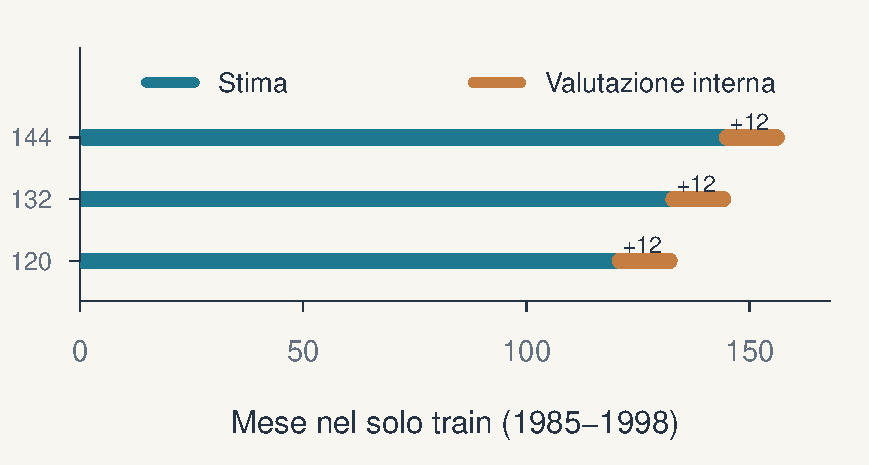
\includegraphics[width=9.85cm,height=5.25cm,keepaspectratio]{Risultati/Figure/06_cv_origini.pdf}
\vspace{1.5mm}
\PSmall{Calendario delle origini interne e delle rispettive verifiche a 12 mesi.}

\end{minipage}\end{lrbox}
\typeout{FULLBOX:073:PilotLeftBox:\the\ht\PilotLeftBox:\the\dp\PilotLeftBox}

\begin{lrbox}{\PilotRightBox}
\begin{minipage}[t]{7.55cm}\raggedright\color{Ink}\fontsize{11.3}{14.8}\selectfont
\PBody{Il confronto conserva una riga per coppia origine--orizzonte, con osservazione, previsione del SARIMA e riferimenti.}
\vspace{2.5mm}
\PInfo{Le tre finestre future sono distinte, ma i train sono sovrapposti. Le stime e i loro errori non diventano automaticamente repliche indipendenti.}
\PCode{R · struttura della validazione}{073_esempio.R}
\end{minipage}\end{lrbox}
\typeout{FULLBOX:073:PilotRightBox:\the\ht\PilotRightBox:\the\dp\PilotRightBox}

\begin{tikzpicture}[remember picture,overlay]
\PilotChrome{Tre origini e trentasei coppie di verifica}{VI · VALIDAZIONE TEMPORALE}{73}{Il numero di righe non coincide necessariamente con il numero di repliche statisticamente indipendenti.}
\node[anchor=north west,inner sep=0] at([xshift=.96cm,yshift=-2.13cm]current page.north west){\usebox{\PilotLeftBox}};
\node[anchor=north west,inner sep=0] at([xshift=11.52cm,yshift=-2.13cm]current page.north west){\usebox{\PilotRightBox}};
\node[anchor=north east,inner sep=0] at([xshift=17.65cm,yshift=-12.06cm]current page.north west){\color{Classical}\fontsize{7.7}{9.2}\selectfont\href{../../03_Notebook_svolti/M10_Futura/M10_N05.html}{M10\_N05 · notebook svolto}};
\end{tikzpicture}\end{frame}

\begin{frame}[plain]\hypertarget{slide74}{}
\bookmark[level=1,page=74]{Tutta la procedura va ripetuta dentro ogni origine}
\begin{lrbox}{\TitleBox}
\begin{minipage}[t]{17.7cm}\raggedright\color{Ink}\fontsize{11.3}{14.8}\selectfont
\color{Navy}\bfseries\fontsize{20.6}{24.5}\selectfont Tutta la procedura va ripetuta dentro ogni origine
\end{minipage}\end{lrbox}
\typeout{FULLBOX:074:TitleBox:\the\ht\TitleBox:\the\dp\TitleBox}

\begin{lrbox}{\RecallBox}
\begin{minipage}[t]{14.3cm}\raggedright\color{Ink}\fontsize{11.3}{14.8}\selectfont
\fontsize{10.3}{13.8}\selectfont La validazione riguarda una procedura intera, non soltanto l’ultima chiamata di previsione.
\end{minipage}\end{lrbox}
\typeout{FULLBOX:074:RecallBox:\the\ht\RecallBox:\the\dp\RecallBox}

\begin{lrbox}{\PilotLeftBox}
\begin{minipage}[t]{10.05cm}\raggedright\color{Ink}\fontsize{11.3}{14.8}\selectfont
\begin{tikzpicture}[x=1cm,y=1cm]
\path[use as bounding box](-.1,-.15) rectangle(9.7,4.8);
\node[pFlow,text width=3.6cm,fill=GeoA!7] (a) at(2.1,3.65){Passato disponibile\\alla singola origine};
\node[pFlow,text width=3.6cm,fill=GeoC!7] (b) at(7.4,3.65){Trasformazioni\\e stima};
\node[pFlow,text width=3.6cm,fill=GeoB!7] (c) at(2.1,1.15){Errore sui mesi\\successivi};
\node[pFlow,text width=3.6cm,fill=GeoB!7] (d) at(7.4,1.15){Previsione\\per quei mesi};
\draw[pEdge] (a) -- (b);
\draw[pEdge] (b) -- (d);
\draw[pEdge] (d) -- (c);
\end{tikzpicture}

\end{minipage}\end{lrbox}
\typeout{FULLBOX:074:PilotLeftBox:\the\ht\PilotLeftBox:\the\dp\PilotLeftBox}

\begin{lrbox}{\PilotRightBox}
\begin{minipage}[t]{7.55cm}\raggedright\color{Ink}\fontsize{11.3}{14.8}\selectfont
\PBody{Se una trasformazione stima media, scala, parametri di imputazione o componenti, deve essere appresa dal train della singola origine.}
\vspace{2.5mm}
\PInfo{Una normalizzazione stimata sull’intera serie trasferirebbe informazioni del futuro nella procedura interna.}
\PBody{Il protocollo conserva la specifica SARIMA, ma ricalcola i coefficienti per ogni passato disponibile.}
\vspace{2.5mm}

\end{minipage}\end{lrbox}
\typeout{FULLBOX:074:PilotRightBox:\the\ht\PilotRightBox:\the\dp\PilotRightBox}

\begin{tikzpicture}[remember picture,overlay]
\PilotChrome{Tutta la procedura va ripetuta dentro ogni origine}{VI · VALIDAZIONE TEMPORALE}{74}{La validazione riguarda una procedura intera, non soltanto l’ultima chiamata di previsione.}
\node[anchor=north west,inner sep=0] at([xshift=.96cm,yshift=-2.13cm]current page.north west){\usebox{\PilotLeftBox}};
\node[anchor=north west,inner sep=0] at([xshift=11.52cm,yshift=-2.13cm]current page.north west){\usebox{\PilotRightBox}};
\end{tikzpicture}\end{frame}

\begin{frame}[plain]\hypertarget{slide75}{}
\bookmark[level=1,page=75]{La dispersione fra origini è parte del risultato}
\begin{lrbox}{\TitleBox}
\begin{minipage}[t]{17.7cm}\raggedright\color{Ink}\fontsize{11.3}{14.8}\selectfont
\color{Navy}\bfseries\fontsize{20.6}{24.5}\selectfont La dispersione fra origini è parte del risultato
\end{minipage}\end{lrbox}
\typeout{FULLBOX:075:TitleBox:\the\ht\TitleBox:\the\dp\TitleBox}

\begin{lrbox}{\RecallBox}
\begin{minipage}[t]{14.3cm}\raggedright\color{Ink}\fontsize{11.3}{14.8}\selectfont
\fontsize{10.3}{13.8}\selectfont La prestazione deve essere accompagnata dal periodo e dalla variabilità fra situazioni valutate.
\end{minipage}\end{lrbox}
\typeout{FULLBOX:075:RecallBox:\the\ht\RecallBox:\the\dp\RecallBox}

\begin{lrbox}{\PilotLeftBox}
\begin{minipage}[t]{10.05cm}\raggedright\color{Ink}\fontsize{11.3}{14.8}\selectfont
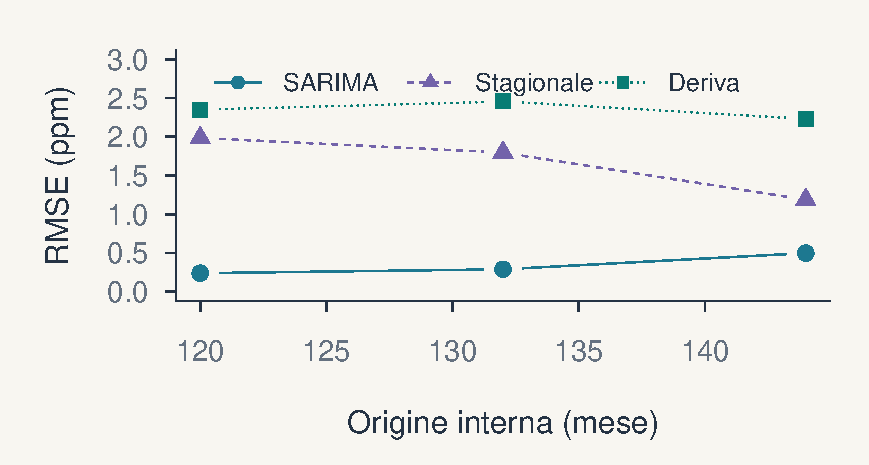
\includegraphics[width=9.85cm,height=5.25cm,keepaspectratio]{Risultati/Figure/07_cv_RMSE.pdf}
\vspace{1.5mm}
\PSmall{RMSE sui 12 mesi successivi a ciascuna origine; confronti sulla stessa scala in ppm.}

\end{minipage}\end{lrbox}
\typeout{FULLBOX:075:PilotLeftBox:\the\ht\PilotLeftBox:\the\dp\PilotLeftBox}

\begin{lrbox}{\PilotRightBox}
\begin{minipage}[t]{7.55cm}\raggedright\color{Ink}\fontsize{11.3}{14.8}\selectfont
\PBody{Una media complessiva può nascondere origini facili e difficili. Il grafico mostra se un vantaggio è stabile oppure concentrato in una sola finestra.}
\vspace{2.5mm}
\PInfo{Tre origini sono poche per descrivere la variabilità delle prestazioni. Il risultato sostiene una valutazione locale del protocollo.}
\PSmall{Si riportano i valori per origine e i riferimenti, evitando di presentare un solo numero come proprietà generale del modello.}

\end{minipage}\end{lrbox}
\typeout{FULLBOX:075:PilotRightBox:\the\ht\PilotRightBox:\the\dp\PilotRightBox}

\begin{tikzpicture}[remember picture,overlay]
\PilotChrome{La dispersione fra origini è parte del risultato}{VI · VALIDAZIONE TEMPORALE}{75}{La prestazione deve essere accompagnata dal periodo e dalla variabilità fra situazioni valutate.}
\node[anchor=north west,inner sep=0] at([xshift=.96cm,yshift=-2.13cm]current page.north west){\usebox{\PilotLeftBox}};
\node[anchor=north west,inner sep=0] at([xshift=11.52cm,yshift=-2.13cm]current page.north west){\usebox{\PilotRightBox}};
\end{tikzpicture}\end{frame}

\begin{frame}[plain]\hypertarget{slide76}{}
\bookmark[level=1,page=76]{La tabella interna tiene separati i metodi}
\begin{lrbox}{\TitleBox}
\begin{minipage}[t]{17.7cm}\raggedright\color{Ink}\fontsize{11.3}{14.8}\selectfont
\color{Navy}\bfseries\fontsize{20.6}{24.5}\selectfont La tabella interna tiene separati i metodi
\end{minipage}\end{lrbox}
\typeout{FULLBOX:076:TitleBox:\the\ht\TitleBox:\the\dp\TitleBox}

\begin{lrbox}{\RecallBox}
\begin{minipage}[t]{14.3cm}\raggedright\color{Ink}\fontsize{11.3}{14.8}\selectfont
\fontsize{10.3}{13.8}\selectfont Il confronto è equo quando origine, orizzonte, osservazioni e metrica sono gli stessi.
\end{minipage}\end{lrbox}
\typeout{FULLBOX:076:RecallBox:\the\ht\RecallBox:\the\dp\RecallBox}

\begin{lrbox}{\PilotLeftBox}
\begin{minipage}[t]{10.05cm}\raggedright\color{Ink}\fontsize{11.3}{14.8}\selectfont
{\fontsize{10.2}{13.1}\selectfont\renewcommand{\arraystretch}{1.45}\begin{tabular}{@{}p{2.0835cm}p{2.0835cm}p{2.0835cm}p{2.0835cm}@{}}\toprule
\textbf{Origine} & \textbf{SARIMA} & \textbf{Stagionale} & \textbf{Deriva}\\\midrule
120 & 0,239 & 1,985 & 2,349\\
132 & 0,289 & 1,794 & 2,456\\
144 & 0,498 & 1,188 & 2,231\\
\bottomrule\end{tabular}}
\PSmall{RMSE in ppm. Origini 120, 132 e 144: dicembre 1994, dicembre 1995 e dicembre 1996.}

\end{minipage}\end{lrbox}
\typeout{FULLBOX:076:PilotLeftBox:\the\ht\PilotLeftBox:\the\dp\PilotLeftBox}

\begin{lrbox}{\PilotRightBox}
\begin{minipage}[t]{7.55cm}\raggedright\color{Ink}\fontsize{11.3}{14.8}\selectfont
\PBody{I metodi sono valutati sugli stessi mesi futuri di ogni origine. Nessuna cella usa il test 1999--2001.}
\vspace{2.5mm}
\PInfo{La graduatoria interna è un’evidenza sul compito a 12 mesi. Non dimostra da sola il comportamento a 36 mesi.}
\PBody{Se si modifica una scelta in base a questa tabella, la modifica resta parte dello sviluppo sul train.}
\vspace{2.5mm}

\end{minipage}\end{lrbox}
\typeout{FULLBOX:076:PilotRightBox:\the\ht\PilotRightBox:\the\dp\PilotRightBox}

\begin{tikzpicture}[remember picture,overlay]
\PilotChrome{La tabella interna tiene separati i metodi}{VI · VALIDAZIONE TEMPORALE}{76}{Il confronto è equo quando origine, orizzonte, osservazioni e metrica sono gli stessi.}
\node[anchor=north west,inner sep=0] at([xshift=.96cm,yshift=-2.13cm]current page.north west){\usebox{\PilotLeftBox}};
\node[anchor=north west,inner sep=0] at([xshift=11.52cm,yshift=-2.13cm]current page.north west){\usebox{\PilotRightBox}};
\end{tikzpicture}\end{frame}

\begin{frame}[plain]\hypertarget{slide77}{}
\bookmark[level=1,page=77]{Un approfondimento usa trentasette origini mensili}
\begin{lrbox}{\TitleBox}
\begin{minipage}[t]{17.7cm}\raggedright\color{Ink}\fontsize{11.3}{14.8}\selectfont
\color{Navy}\bfseries\fontsize{20.6}{24.5}\selectfont Un approfondimento usa trentasette origini mensili
\end{minipage}\end{lrbox}
\typeout{FULLBOX:077:TitleBox:\the\ht\TitleBox:\the\dp\TitleBox}

\begin{lrbox}{\RecallBox}
\begin{minipage}[t]{14.3cm}\raggedright\color{Ink}\fontsize{11.3}{14.8}\selectfont
\fontsize{10.3}{13.8}\selectfont Più origini offrono una descrizione più ricca, ma la sovrapposizione va dichiarata.
\end{minipage}\end{lrbox}
\typeout{FULLBOX:077:RecallBox:\the\ht\RecallBox:\the\dp\RecallBox}

\begin{lrbox}{\PilotLeftBox}
\begin{minipage}[t]{10.05cm}\raggedright\color{Ink}\fontsize{11.3}{14.8}\selectfont
\begin{tikzpicture}[x=1cm,y=1cm]
\path[use as bounding box](-.1,-.15) rectangle(9.7,4.9);
\fill[GeoA!20](.5,3.96)rectangle(5.500,4.44);
\fill[GeoB!40](5.500,3.96)rectangle(6.000,4.44);
\node[pNote,anchor=west]at(6.160,4.2){120};
\fill[GeoA!20](.5,3.04)rectangle(6.000,3.5200000000000005);
\fill[GeoB!40](6.000,3.04)rectangle(6.500,3.5200000000000005);
\node[pNote,anchor=west]at(6.660,3.2800000000000002){132};
\fill[GeoA!20](.5,2.12)rectangle(6.500,2.6000000000000005);
\fill[GeoB!40](6.500,2.12)rectangle(7.000,2.6000000000000005);
\node[pNote,anchor=west]at(7.160,2.3600000000000003){144};
\fill[GeoA!20](.5,1.2)rectangle(7.000,1.68);
\fill[GeoB!40](7.000,1.2)rectangle(7.500,1.68);
\node[pNote,anchor=west]at(7.660,1.44){156};
\draw[Muted,dashed](7.500,.6)--(7.500,4.65);
\node[pNote]at(4,.25){train in verde · verifica interna in rame};
\node[pNote]at(8.8,4.4){test\\finale};
\end{tikzpicture}
\[o=120,121,\ldots,156,\qquad h=1,\ldots,12\]

\end{minipage}\end{lrbox}
\typeout{FULLBOX:077:PilotLeftBox:\the\ht\PilotLeftBox:\the\dp\PilotLeftBox}

\begin{lrbox}{\PilotRightBox}
\begin{minipage}[t]{7.55cm}\raggedright\color{Ink}\fontsize{11.3}{14.8}\selectfont
\PBody{L’approfondimento aggiunge 37 origini e 444 coppie origine--orizzonte, tutte interne ai primi 168 mesi. Serve a osservare il comportamento per orizzonte.}
\vspace{2.5mm}
\PInfo{Le verifiche si sovrappongono. La stessa osservazione può comparire come futuro a orizzonti diversi: non si tratta di 444 casi indipendenti.}
\PSmall{Questo ampliamento è distinto dalle tre origini del protocollo ripreso dal sito.}

\end{minipage}\end{lrbox}
\typeout{FULLBOX:077:PilotRightBox:\the\ht\PilotRightBox:\the\dp\PilotRightBox}

\begin{tikzpicture}[remember picture,overlay]
\PilotChrome{Un approfondimento usa trentasette origini mensili}{VI · VALIDAZIONE TEMPORALE}{77}{Più origini offrono una descrizione più ricca, ma la sovrapposizione va dichiarata.}
\node[anchor=north west,inner sep=0] at([xshift=.96cm,yshift=-2.13cm]current page.north west){\usebox{\PilotLeftBox}};
\node[anchor=north west,inner sep=0] at([xshift=11.52cm,yshift=-2.13cm]current page.north west){\usebox{\PilotRightBox}};
\end{tikzpicture}\end{frame}

\begin{frame}[plain]\hypertarget{slide78}{}
\bookmark[level=1,page=78]{L’errore può cambiare con l’orizzonte}
\begin{lrbox}{\TitleBox}
\begin{minipage}[t]{17.7cm}\raggedright\color{Ink}\fontsize{11.3}{14.8}\selectfont
\color{Navy}\bfseries\fontsize{20.6}{24.5}\selectfont L’errore può cambiare con l’orizzonte
\end{minipage}\end{lrbox}
\typeout{FULLBOX:078:TitleBox:\the\ht\TitleBox:\the\dp\TitleBox}

\begin{lrbox}{\RecallBox}
\begin{minipage}[t]{14.3cm}\raggedright\color{Ink}\fontsize{11.3}{14.8}\selectfont
\fontsize{10.3}{13.8}\selectfont L’orizzonte è parte del risultato, non una semplice etichetta della previsione.
\end{minipage}\end{lrbox}
\typeout{FULLBOX:078:RecallBox:\the\ht\RecallBox:\the\dp\RecallBox}

\begin{lrbox}{\PilotLeftBox}
\begin{minipage}[t]{10.05cm}\raggedright\color{Ink}\fontsize{11.3}{14.8}\selectfont
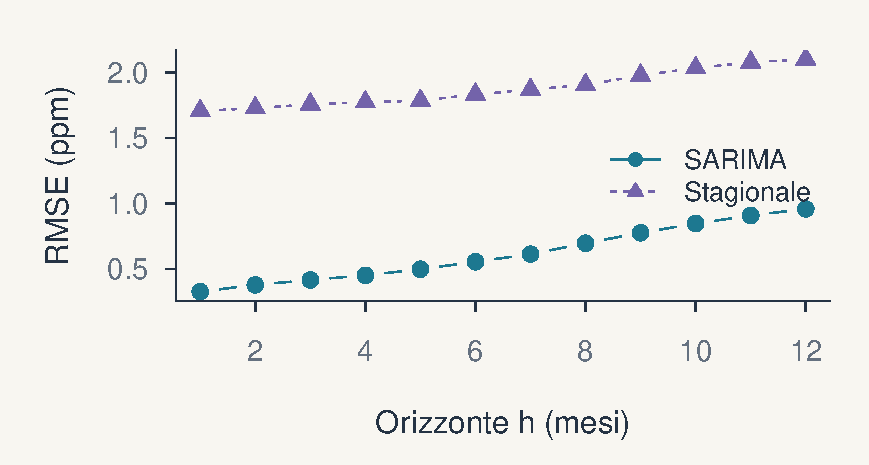
\includegraphics[width=9.85cm,height=5.25cm,keepaspectratio]{Risultati/Figure/35_rolling_orizzonte.pdf}
\vspace{1.5mm}
\PSmall{Approfondimento: 37 origini mensili, sempre nel train. Ogni orizzonte riassume 37 previsioni.}

\end{minipage}\end{lrbox}
\typeout{FULLBOX:078:PilotLeftBox:\the\ht\PilotLeftBox:\the\dp\PilotLeftBox}

\begin{lrbox}{\PilotRightBox}
\begin{minipage}[t]{7.55cm}\raggedright\color{Ink}\fontsize{11.3}{14.8}\selectfont
\PBody{Un modello può essere competitivo a un mese e perdere vantaggio a un anno. Per questo una metrica aggregata su più orizzonti non basta a descrivere ogni uso.}
\vspace{2.5mm}
\PInfo{Le curve sono descrittive e riguardano questo archivio. La dipendenza fra origini impedisce di leggere le differenze come se fossero medie di repliche indipendenti.}

\end{minipage}\end{lrbox}
\typeout{FULLBOX:078:PilotRightBox:\the\ht\PilotRightBox:\the\dp\PilotRightBox}

\begin{tikzpicture}[remember picture,overlay]
\PilotChrome{L’errore può cambiare con l’orizzonte}{VI · VALIDAZIONE TEMPORALE}{78}{L’orizzonte è parte del risultato, non una semplice etichetta della previsione.}
\node[anchor=north west,inner sep=0] at([xshift=.96cm,yshift=-2.13cm]current page.north west){\usebox{\PilotLeftBox}};
\node[anchor=north west,inner sep=0] at([xshift=11.52cm,yshift=-2.13cm]current page.north west){\usebox{\PilotRightBox}};
\end{tikzpicture}\end{frame}

\begin{frame}[plain]\hypertarget{slide79}{}
\bookmark[level=1,page=79]{La mappa degli errori distingue periodo e orizzonte}
\begin{lrbox}{\TitleBox}
\begin{minipage}[t]{17.7cm}\raggedright\color{Ink}\fontsize{11.3}{14.8}\selectfont
\color{Navy}\bfseries\fontsize{20.6}{24.5}\selectfont La mappa degli errori distingue periodo e orizzonte
\end{minipage}\end{lrbox}
\typeout{FULLBOX:079:TitleBox:\the\ht\TitleBox:\the\dp\TitleBox}

\begin{lrbox}{\RecallBox}
\begin{minipage}[t]{14.3cm}\raggedright\color{Ink}\fontsize{11.3}{14.8}\selectfont
\fontsize{10.3}{13.8}\selectfont Una vista con origine e orizzonte permette di localizzare le difficoltà del modello.
\end{minipage}\end{lrbox}
\typeout{FULLBOX:079:RecallBox:\the\ht\RecallBox:\the\dp\RecallBox}

\begin{lrbox}{\PilotLeftBox}
\begin{minipage}[t]{10.05cm}\raggedright\color{Ink}\fontsize{11.3}{14.8}\selectfont
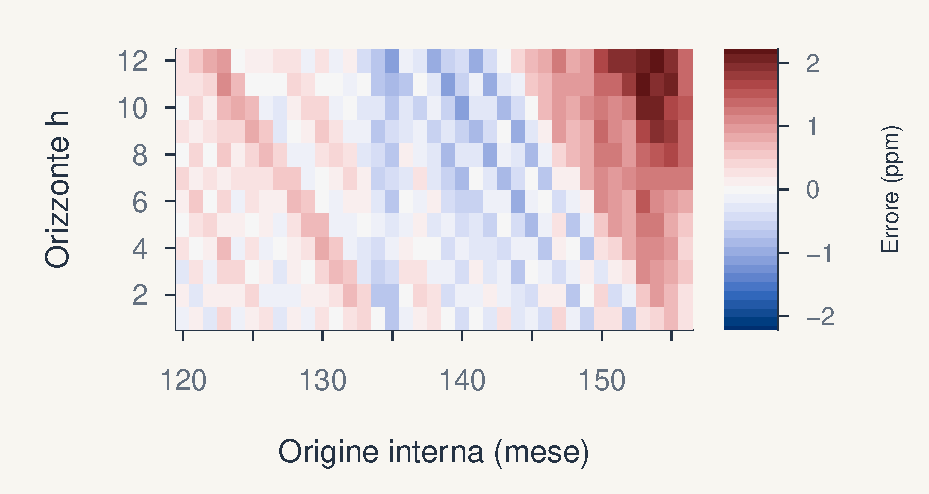
\includegraphics[width=9.85cm,height=5.25cm,keepaspectratio]{Risultati/Figure/36_rolling_errori.pdf}
\vspace{1.5mm}
\PSmall{Errore osservato meno previsto; scala cromatica simmetrica. Origini e orizzonti sono distinti.}

\end{minipage}\end{lrbox}
\typeout{FULLBOX:079:PilotLeftBox:\the\ht\PilotLeftBox:\the\dp\PilotLeftBox}

\begin{lrbox}{\PilotRightBox}
\begin{minipage}[t]{7.55cm}\raggedright\color{Ink}\fontsize{11.3}{14.8}\selectfont
\PBody{Bande verticali o orizzontali possono indicare periodi difficili o orizzonti problematici. Il segno aiuta a riconoscere sottostima e sovrastima.}
\vspace{2.5mm}
\PInfo{Una struttura visiva suggerisce una domanda. Non identifica automaticamente un cambiamento fisico o una causa.}
\PSmall{Il grafico conserva le 444 coppie, mentre una singola RMSE ne ridurrebbe tutta l’informazione a uno scalare.}

\end{minipage}\end{lrbox}
\typeout{FULLBOX:079:PilotRightBox:\the\ht\PilotRightBox:\the\dp\PilotRightBox}

\begin{tikzpicture}[remember picture,overlay]
\PilotChrome{La mappa degli errori distingue periodo e orizzonte}{VI · VALIDAZIONE TEMPORALE}{79}{Una vista con origine e orizzonte permette di localizzare le difficoltà del modello.}
\node[anchor=north west,inner sep=0] at([xshift=.96cm,yshift=-2.13cm]current page.north west){\usebox{\PilotLeftBox}};
\node[anchor=north west,inner sep=0] at([xshift=11.52cm,yshift=-2.13cm]current page.north west){\usebox{\PilotRightBox}};
\end{tikzpicture}\end{frame}

\begin{frame}[plain]\hypertarget{slide80}{}
\bookmark[level=1,page=80]{Il test finale si apre dopo aver fissato la procedura}
\begin{lrbox}{\TitleBox}
\begin{minipage}[t]{17.7cm}\raggedright\color{Ink}\fontsize{11.3}{14.8}\selectfont
\color{Navy}\bfseries\fontsize{20.6}{24.5}\selectfont Il test finale si apre dopo aver fissato la procedura
\end{minipage}\end{lrbox}
\typeout{FULLBOX:080:TitleBox:\the\ht\TitleBox:\the\dp\TitleBox}

\begin{lrbox}{\RecallBox}
\begin{minipage}[t]{14.3cm}\raggedright\color{Ink}\fontsize{11.3}{14.8}\selectfont
\fontsize{10.3}{13.8}\selectfont La separazione tra sviluppo e verifica protegge l’interpretazione della prestazione.
\end{minipage}\end{lrbox}
\typeout{FULLBOX:080:RecallBox:\the\ht\RecallBox:\the\dp\RecallBox}

\begin{lrbox}{\PilotLeftBox}
\begin{minipage}[t]{10.05cm}\raggedright\color{Ink}\fontsize{11.3}{14.8}\selectfont
\begin{tikzpicture}[x=1cm,y=1cm]
\path[use as bounding box](-.1,-.15) rectangle(9.7,4.8);
\fill[GeoA!17](.4,1.7)rectangle(7.2,3.25);
\fill[GeoB!18](7.2,1.7)rectangle(9.4,3.25);
\node[pLabel]at(3.8,2.65){Addestramento: 168 mesi};
\node[pNote]at(3.8,2.05){gennaio 1985 -- dicembre 1998};
\node[pLabel]at(8.3,2.65){Test: 36};
\node[pNote]at(8.3,2.05){1999--2001};
\draw[Classical,line width=1pt](7.2,1.35)--(7.2,3.7);
\node[pLabel,anchor=east]at(7.0,3.7){Origine $T$};
\draw[pAxis](.4,1.2)--(9.5,1.2);
\node[pNote]at(.8,.65){passato};\node[pNote]at(8.5,.65){futuro storico};
\draw[decorate,decoration={brace,amplitude=4pt},GeoB](7.2,4.05)--(9.4,4.05);
\node[pNote]at(8.3,4.45){$h=1,\ldots,36$};
\end{tikzpicture}
\PInfo{La specifica, i riferimenti e le metriche sono registrati prima di leggere i risultati 1999--2001.}

\end{minipage}\end{lrbox}
\typeout{FULLBOX:080:PilotLeftBox:\the\ht\PilotLeftBox:\the\dp\PilotLeftBox}

\begin{lrbox}{\PilotRightBox}
\begin{minipage}[t]{7.55cm}\raggedright\color{Ink}\fontsize{11.3}{14.8}\selectfont
\PBody{Il test finale valuta l’intera procedura sviluppata sul train. Usarlo ripetutamente per scegliere varianti lo trasforma in un ulteriore campione di sviluppo.}
\vspace{2.5mm}
\PInfo{Una revisione suggerita dal test può essere scientificamente utile. Va dichiarata come nuova ipotesi e verificata su altro materiale.}
\PBody{La stima finale torna a usare tutti i 168 mesi, con le scelte ormai fissate.}
\vspace{2.5mm}

\end{minipage}\end{lrbox}
\typeout{FULLBOX:080:PilotRightBox:\the\ht\PilotRightBox:\the\dp\PilotRightBox}

\begin{tikzpicture}[remember picture,overlay]
\PilotChrome{Il test finale si apre dopo aver fissato la procedura}{VI · VALIDAZIONE TEMPORALE}{80}{La separazione tra sviluppo e verifica protegge l’interpretazione della prestazione.}
\node[anchor=north west,inner sep=0] at([xshift=.96cm,yshift=-2.13cm]current page.north west){\usebox{\PilotLeftBox}};
\node[anchor=north west,inner sep=0] at([xshift=11.52cm,yshift=-2.13cm]current page.north west){\usebox{\PilotRightBox}};
\end{tikzpicture}\end{frame}

\begin{frame}[plain]\hypertarget{slide81}{}
\bookmark[level=1,page=81]{Verificare la separazione dal test}
\begin{lrbox}{\TitleBox}
\begin{minipage}[t]{17.7cm}\raggedright\color{Ink}\fontsize{11.3}{14.8}\selectfont
\color{Navy}\bfseries\fontsize{20.6}{24.5}\selectfont Verificare la separazione dal test
\end{minipage}\end{lrbox}
\typeout{FULLBOX:081:TitleBox:\the\ht\TitleBox:\the\dp\TitleBox}

\begin{lrbox}{\RecallBox}
\begin{minipage}[t]{14.3cm}\raggedright\color{Ink}\fontsize{11.3}{14.8}\selectfont
\fontsize{10.3}{13.8}\selectfont Un controllo utile prova un rischio concreto e osserva un effetto che deve restare invariato.
\end{minipage}\end{lrbox}
\typeout{FULLBOX:081:RecallBox:\the\ht\RecallBox:\the\dp\RecallBox}

\begin{lrbox}{\PilotLeftBox}
\begin{minipage}[t]{10.05cm}\raggedright\color{Ink}\fontsize{11.3}{14.8}\selectfont
\begin{tikzpicture}[x=1cm,y=1cm]
\path[use as bounding box](-.1,-.15) rectangle(9.7,4.8);
\node[pFlow,text width=3.6cm,fill=GeoB!7] (a) at(2.1,3.5){Copia dei dati\\con test alterato};
\node[pFlow,text width=3.6cm,fill=GeoA!7] (b) at(7.4,3.5){Train estratto\\per calendario};
\node[pFlow,text width=3.6cm,fill=GeoA!7] (c) at(2.1,1.1){Train originale};
\node[pFlow,text width=3.6cm,fill=GeoC!7] (d) at(7.4,1.1){Previsioni\\identiche};
\draw[pEdge] (a) -- (b);
\draw[pEdge] (b) -- (d);
\draw[pEdge] (c) -- (d);
\end{tikzpicture}

\end{minipage}\end{lrbox}
\typeout{FULLBOX:081:PilotLeftBox:\the\ht\PilotLeftBox:\the\dp\PilotLeftBox}

\begin{lrbox}{\PilotRightBox}
\begin{minipage}[t]{7.55cm}\raggedright\color{Ink}\fontsize{11.3}{14.8}\selectfont
\PBody{La verifica automatica altera tutti i 36 valori futuri e ripete l’estrazione del train. Train, riferimenti e previsione SARIMA devono rimanere identici.}
\vspace{2.5mm}
\PInfo{Il controllo rileva una dipendenza accidentale dai valori del test nel procedimento implementato. Non sostituisce la revisione delle scelte fatte dall’analista.}
\PCode{R · separazione del calendario}{081_esempio.R}
\end{minipage}\end{lrbox}
\typeout{FULLBOX:081:PilotRightBox:\the\ht\PilotRightBox:\the\dp\PilotRightBox}

\begin{tikzpicture}[remember picture,overlay]
\PilotChrome{Verificare la separazione dal test}{VI · VALIDAZIONE TEMPORALE}{81}{Un controllo utile prova un rischio concreto e osserva un effetto che deve restare invariato.}
\node[anchor=north west,inner sep=0] at([xshift=.96cm,yshift=-2.13cm]current page.north west){\usebox{\PilotLeftBox}};
\node[anchor=north west,inner sep=0] at([xshift=11.52cm,yshift=-2.13cm]current page.north west){\usebox{\PilotRightBox}};
\end{tikzpicture}\end{frame}

\begin{frame}[plain]\hypertarget{slide82}{}
\bookmark[level=1,page=82]{Laboratorio: il disegno prima del punteggio}
\begin{lrbox}{\TitleBox}
\begin{minipage}[t]{17.7cm}\raggedright\color{Ink}\fontsize{11.3}{14.8}\selectfont
\color{Navy}\bfseries\fontsize{20.6}{24.5}\selectfont Laboratorio: il disegno prima del punteggio
\end{minipage}\end{lrbox}
\typeout{FULLBOX:082:TitleBox:\the\ht\TitleBox:\the\dp\TitleBox}

\begin{lrbox}{\RecallBox}
\begin{minipage}[t]{14.3cm}\raggedright\color{Ink}\fontsize{11.3}{14.8}\selectfont
\fontsize{10.3}{13.8}\selectfont Una metrica senza il disegno di validazione non è un risultato interpretabile.
\end{minipage}\end{lrbox}
\typeout{FULLBOX:082:RecallBox:\the\ht\RecallBox:\the\dp\RecallBox}

\begin{lrbox}{\PilotLeftBox}
\begin{minipage}[t]{10.05cm}\raggedright\color{Ink}\fontsize{11.3}{14.8}\selectfont
{\fontsize{10.2}{13.1}\selectfont\renewcommand{\arraystretch}{1.45}\begin{tabular}{@{}p{3.5cm}p{5.5cm}@{}}\toprule
\textbf{Da dichiarare} & \textbf{Protocollo principale}\\\midrule
Origini & 120, 132, 144\\
Finestra & Crescente, da gennaio 1985\\
Orizzonte interno & 12 mesi\\
Aggiornamento & Nuova stima per origine\\
Test finale & 36 mesi a origine fissa\\
Limite & Poche origini e errori dipendenti\\
\bottomrule\end{tabular}}

\end{minipage}\end{lrbox}
\typeout{FULLBOX:082:PilotLeftBox:\the\ht\PilotLeftBox:\the\dp\PilotLeftBox}

\begin{lrbox}{\PilotRightBox}
\begin{minipage}[t]{7.55cm}\raggedright\color{Ink}\fontsize{11.3}{14.8}\selectfont
\PBody{M10\_N05 produce la tabella per origine. Il rapporto deve spiegare come sono stati ottenuti i numeri, oltre a indicare il modello con l’errore minore.}
\vspace{2.5mm}
\PInfo{L’approfondimento con 37 origini non cambia il protocollo centrale. Serve a esplorare il rapporto fra orizzonte e prestazione.}

\end{minipage}\end{lrbox}
\typeout{FULLBOX:082:PilotRightBox:\the\ht\PilotRightBox:\the\dp\PilotRightBox}

\begin{tikzpicture}[remember picture,overlay]
\PilotChrome{Laboratorio: il disegno prima del punteggio}{VI · VALIDAZIONE TEMPORALE}{82}{Una metrica senza il disegno di validazione non è un risultato interpretabile.}
\node[anchor=north west,inner sep=0] at([xshift=.96cm,yshift=-2.13cm]current page.north west){\usebox{\PilotLeftBox}};
\node[anchor=north west,inner sep=0] at([xshift=11.52cm,yshift=-2.13cm]current page.north west){\usebox{\PilotRightBox}};
\node[anchor=north east,inner sep=0] at([xshift=17.65cm,yshift=-12.06cm]current page.north west){\color{Classical}\fontsize{7.7}{9.2}\selectfont\href{../../03_Notebook_svolti/M10_Futura/M10_N05.html}{M10\_N05 · notebook svolto}};
\end{tikzpicture}\end{frame}

\begin{frame}[plain]\hypertarget{slide83}{}
\bookmark[level=0,page=83]{VII · ERRORI E INTERVALLI}
\bookmark[level=1,page=83]{Prima delle metriche si controllano date e segno}
\begin{lrbox}{\TitleBox}
\begin{minipage}[t]{17.7cm}\raggedright\color{Ink}\fontsize{11.3}{14.8}\selectfont
\color{Navy}\bfseries\fontsize{20.6}{24.5}\selectfont Prima delle metriche si controllano date e segno
\end{minipage}\end{lrbox}
\typeout{FULLBOX:083:TitleBox:\the\ht\TitleBox:\the\dp\TitleBox}

\begin{lrbox}{\RecallBox}
\begin{minipage}[t]{14.3cm}\raggedright\color{Ink}\fontsize{11.3}{14.8}\selectfont
\fontsize{10.3}{13.8}\selectfont Una metrica corretta richiede coppie temporali corrette.
\end{minipage}\end{lrbox}
\typeout{FULLBOX:083:RecallBox:\the\ht\RecallBox:\the\dp\RecallBox}

\begin{lrbox}{\PilotLeftBox}
\begin{minipage}[t]{10.05cm}\raggedright\color{Ink}\fontsize{11.3}{14.8}\selectfont
\[e_h=y_{T+h}-\widehat y_{T+h\mid T}\]
{\fontsize{10.2}{13.1}\selectfont\renewcommand{\arraystretch}{1.45}\begin{tabular}{@{}p{2.8cm}p{6.3cm}@{}}\toprule
\textbf{Segno} & \textbf{Interpretazione}\\\midrule
$e_h>0$ & Il modello ha sottostimato\\
$e_h<0$ & Il modello ha sovrastimato\\
$e_h=0$ & Previsione e osservazione coincidono\\
\bottomrule\end{tabular}}

\end{minipage}\end{lrbox}
\typeout{FULLBOX:083:PilotLeftBox:\the\ht\PilotLeftBox:\the\dp\PilotLeftBox}

\begin{lrbox}{\PilotRightBox}
\begin{minipage}[t]{7.55cm}\raggedright\color{Ink}\fontsize{11.3}{14.8}\selectfont
\PBody{La convenzione osservato meno previsto viene mantenuta in tutte le tabelle. Il confronto richiede la stessa data, la stessa unità e vettori della stessa lunghezza.}
\vspace{2.5mm}
\PInfo{R può riciclare vettori di lunghezze differenti. Un controllo esplicito evita che un errore di struttura produca una metrica apparentemente valida.}
\PCode{R · errore osservato meno previsto}{083_esempio.R}
\end{minipage}\end{lrbox}
\typeout{FULLBOX:083:PilotRightBox:\the\ht\PilotRightBox:\the\dp\PilotRightBox}

\begin{tikzpicture}[remember picture,overlay]
\PilotChrome{Prima delle metriche si controllano date e segno}{VII · ERRORI E INTERVALLI}{83}{Una metrica corretta richiede coppie temporali corrette.}
\node[anchor=north west,inner sep=0] at([xshift=.96cm,yshift=-2.13cm]current page.north west){\usebox{\PilotLeftBox}};
\node[anchor=north west,inner sep=0] at([xshift=11.52cm,yshift=-2.13cm]current page.north west){\usebox{\PilotRightBox}};
\node[anchor=north east,inner sep=0] at([xshift=17.65cm,yshift=-12.06cm]current page.north west){\color{Classical}\fontsize{7.7}{9.2}\selectfont\href{../../03_Notebook_svolti/M10_Futura/M10_N07.html}{M10\_N07 · notebook svolto}};
\end{tikzpicture}\end{frame}

\begin{frame}[plain]\hypertarget{slide84}{}
\bookmark[level=1,page=84]{MAE, RMSE e bias rispondono a domande diverse}
\begin{lrbox}{\TitleBox}
\begin{minipage}[t]{17.7cm}\raggedright\color{Ink}\fontsize{11.3}{14.8}\selectfont
\color{Navy}\bfseries\fontsize{20.6}{24.5}\selectfont MAE, RMSE e bias rispondono a domande diverse
\end{minipage}\end{lrbox}
\typeout{FULLBOX:084:TitleBox:\the\ht\TitleBox:\the\dp\TitleBox}

\begin{lrbox}{\RecallBox}
\begin{minipage}[t]{14.3cm}\raggedright\color{Ink}\fontsize{11.3}{14.8}\selectfont
\fontsize{10.3}{13.8}\selectfont Dimensione dell’errore e direzione dello scostamento richiedono riassunti distinti.
\end{minipage}\end{lrbox}
\typeout{FULLBOX:084:RecallBox:\the\ht\RecallBox:\the\dp\RecallBox}

\begin{lrbox}{\PilotLeftBox}
\begin{minipage}[t]{10.05cm}\raggedright\color{Ink}\fontsize{11.3}{14.8}\selectfont
\[\operatorname{MAE}=\frac{1}{H}\sum_{h=1}^H|e_h|\]
\[\operatorname{RMSE}=\sqrt{\frac{1}{H}\sum_{h=1}^He_h^2}\]
\[\operatorname{bias}=\frac{1}{H}\sum_{h=1}^He_h\]

\end{minipage}\end{lrbox}
\typeout{FULLBOX:084:PilotLeftBox:\the\ht\PilotLeftBox:\the\dp\PilotLeftBox}

\begin{lrbox}{\PilotRightBox}
\begin{minipage}[t]{7.55cm}\raggedright\color{Ink}\fontsize{11.3}{14.8}\selectfont
\PBody{MAE misura la dimensione media dell’errore assoluto. RMSE attribuisce più peso agli errori grandi. Il bias conserva il segno e rileva uno scostamento sistematico medio.}
\vspace{2.5mm}
\PInfo{Tutte e tre sono in ppm. Un bias piccolo può nascondere errori grandi di segno opposto; non sostituisce MAE o RMSE.}
\PCode{R · tre metriche complementari}{084_esempio.R}
\end{minipage}\end{lrbox}
\typeout{FULLBOX:084:PilotRightBox:\the\ht\PilotRightBox:\the\dp\PilotRightBox}

\begin{tikzpicture}[remember picture,overlay]
\PilotChrome{MAE, RMSE e bias rispondono a domande diverse}{VII · ERRORI E INTERVALLI}{84}{Dimensione dell’errore e direzione dello scostamento richiedono riassunti distinti.}
\node[anchor=north west,inner sep=0] at([xshift=.96cm,yshift=-2.13cm]current page.north west){\usebox{\PilotLeftBox}};
\node[anchor=north west,inner sep=0] at([xshift=11.52cm,yshift=-2.13cm]current page.north west){\usebox{\PilotRightBox}};
\node[anchor=north east,inner sep=0] at([xshift=17.65cm,yshift=-12.06cm]current page.north west){\color{Classical}\fontsize{7.7}{9.2}\selectfont\href{../../03_Notebook_svolti/M10_Futura/M10_N07.html}{M10\_N07 · notebook svolto}};
\end{tikzpicture}\end{frame}

\begin{frame}[plain]\hypertarget{slide85}{}
\bookmark[level=1,page=85]{Il test storico misura il vantaggio sui riferimenti}
\begin{lrbox}{\TitleBox}
\begin{minipage}[t]{17.7cm}\raggedright\color{Ink}\fontsize{11.3}{14.8}\selectfont
\color{Navy}\bfseries\fontsize{20.6}{24.5}\selectfont Il test storico misura il vantaggio sui riferimenti
\end{minipage}\end{lrbox}
\typeout{FULLBOX:085:TitleBox:\the\ht\TitleBox:\the\dp\TitleBox}

\begin{lrbox}{\RecallBox}
\begin{minipage}[t]{14.3cm}\raggedright\color{Ink}\fontsize{11.3}{14.8}\selectfont
\fontsize{10.3}{13.8}\selectfont La prestazione è una proprietà del modello insieme al compito e al campione di verifica.
\end{minipage}\end{lrbox}
\typeout{FULLBOX:085:RecallBox:\the\ht\RecallBox:\the\dp\RecallBox}

\begin{lrbox}{\PilotLeftBox}
\begin{minipage}[t]{10.05cm}\raggedright\color{Ink}\fontsize{11.3}{14.8}\selectfont
\PLabel{Stessa origine, stessi 36 mesi, unità ppm}
{\fontsize{10.2}{13.1}\selectfont\renewcommand{\arraystretch}{1.45}\begin{tabular}{@{}p{2.0835cm}p{2.0835cm}p{2.0835cm}p{2.0835cm}@{}}\toprule
\textbf{Metodo} & \textbf{MAE} & \textbf{RMSE} & \textbf{Bias}\\\midrule
Media & 13,640 & 13,808 & 13,640\\
Ultimo & 2,839 & 3,336 & 2,555\\
Stagionale & 2,866 & 3,109 & 2,866\\
Deriva & 1,884 & 2,148 & 0,118\\
SARIMA & 0,974 & 1,062 & -0,968\\
\bottomrule\end{tabular}}
\PSmall{Bias = osservato meno previsto. Nessuna scelta del modello è aggiornata usando questa graduatoria.}

\end{minipage}\end{lrbox}
\typeout{FULLBOX:085:PilotLeftBox:\the\ht\PilotLeftBox:\the\dp\PilotLeftBox}

\begin{lrbox}{\PilotRightBox}
\begin{minipage}[t]{7.55cm}\raggedright\color{Ink}\fontsize{11.3}{14.8}\selectfont
\PBody{Il SARIMA migliora i riferimenti nel test dichiarato. La deriva è un confronto più esigente del ciclo stagionale ripetuto perché rappresenta una crescita del livello.}
\vspace{2.5mm}
\PInfo{Il vantaggio riguarda l’archivio, l’origine e gli orizzonti indicati. Non equivale a una garanzia per un’altra serie o per un’altra epoca.}
\PSmall{La tabella è letta direttamente dai risultati eseguiti in R.}

\end{minipage}\end{lrbox}
\typeout{FULLBOX:085:PilotRightBox:\the\ht\PilotRightBox:\the\dp\PilotRightBox}

\begin{tikzpicture}[remember picture,overlay]
\PilotChrome{Il test storico misura il vantaggio sui riferimenti}{VII · ERRORI E INTERVALLI}{85}{La prestazione è una proprietà del modello insieme al compito e al campione di verifica.}
\node[anchor=north west,inner sep=0] at([xshift=.96cm,yshift=-2.13cm]current page.north west){\usebox{\PilotLeftBox}};
\node[anchor=north west,inner sep=0] at([xshift=11.52cm,yshift=-2.13cm]current page.north west){\usebox{\PilotRightBox}};
\node[anchor=north east,inner sep=0] at([xshift=17.65cm,yshift=-12.06cm]current page.north west){\color{Classical}\fontsize{7.7}{9.2}\selectfont\href{../../03_Notebook_svolti/M10_Futura/M10_N07.html}{M10\_N07 · notebook svolto}};
\end{tikzpicture}\end{frame}

\begin{frame}[plain]\hypertarget{slide86}{}
\bookmark[level=1,page=86]{Una sovrastima persistente nel test}
\begin{lrbox}{\TitleBox}
\begin{minipage}[t]{17.7cm}\raggedright\color{Ink}\fontsize{11.3}{14.8}\selectfont
\color{Navy}\bfseries\fontsize{20.6}{24.5}\selectfont Una sovrastima persistente nel test
\end{minipage}\end{lrbox}
\typeout{FULLBOX:086:TitleBox:\the\ht\TitleBox:\the\dp\TitleBox}

\begin{lrbox}{\RecallBox}
\begin{minipage}[t]{14.3cm}\raggedright\color{Ink}\fontsize{11.3}{14.8}\selectfont
\fontsize{10.3}{13.8}\selectfont Migliorare un riferimento non significa aver eliminato ogni errore sistematico.
\end{minipage}\end{lrbox}
\typeout{FULLBOX:086:RecallBox:\the\ht\RecallBox:\the\dp\RecallBox}

\begin{lrbox}{\PilotLeftBox}
\begin{minipage}[t]{10.05cm}\raggedright\color{Ink}\fontsize{11.3}{14.8}\selectfont
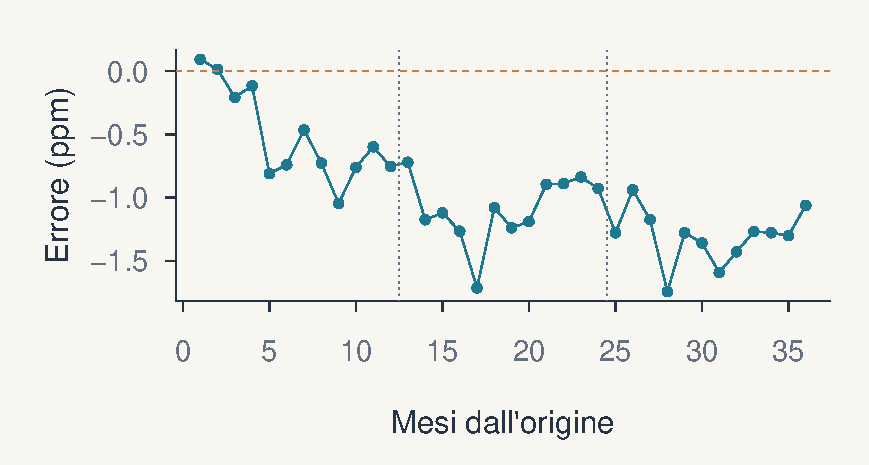
\includegraphics[width=9.85cm,height=5.25cm,keepaspectratio]{Risultati/Figure/04_errori_CO2.pdf}
\vspace{1.5mm}
\PSmall{Sequenza degli errori nel test; valori negativi indicano sovrastima del livello osservato.}

\end{minipage}\end{lrbox}
\typeout{FULLBOX:086:PilotLeftBox:\the\ht\PilotLeftBox:\the\dp\PilotLeftBox}

\begin{lrbox}{\PilotRightBox}
\begin{minipage}[t]{7.55cm}\raggedright\color{Ink}\fontsize{11.3}{14.8}\selectfont
\PBody{Il bias del SARIMA è -0,968 ppm. La buona RMSE rispetto ai riferimenti convive quindi con uno scostamento prevalentemente negativo.}
\vspace{2.5mm}
\PInfo{Un’unica metrica senza segno nasconderebbe questa informazione. La sequenza temporale aiuta a distinguere errori isolati e deviazioni persistenti.}
\PSmall{Una struttura nel test può suggerire nuove ipotesi, da valutare poi con un nuovo protocollo.}

\end{minipage}\end{lrbox}
\typeout{FULLBOX:086:PilotRightBox:\the\ht\PilotRightBox:\the\dp\PilotRightBox}

\begin{tikzpicture}[remember picture,overlay]
\PilotChrome{Una sovrastima persistente nel test}{VII · ERRORI E INTERVALLI}{86}{Migliorare un riferimento non significa aver eliminato ogni errore sistematico.}
\node[anchor=north west,inner sep=0] at([xshift=.96cm,yshift=-2.13cm]current page.north west){\usebox{\PilotLeftBox}};
\node[anchor=north west,inner sep=0] at([xshift=11.52cm,yshift=-2.13cm]current page.north west){\usebox{\PilotRightBox}};
\end{tikzpicture}\end{frame}

\begin{frame}[plain]\hypertarget{slide87}{}
\bookmark[level=1,page=87]{La traiettoria prevista va letta con il suo intervallo}
\begin{lrbox}{\TitleBox}
\begin{minipage}[t]{17.7cm}\raggedright\color{Ink}\fontsize{11.3}{14.8}\selectfont
\color{Navy}\bfseries\fontsize{20.6}{24.5}\selectfont La traiettoria prevista va letta con il suo intervallo
\end{minipage}\end{lrbox}
\typeout{FULLBOX:087:TitleBox:\the\ht\TitleBox:\the\dp\TitleBox}

\begin{lrbox}{\RecallBox}
\begin{minipage}[t]{14.3cm}\raggedright\color{Ink}\fontsize{11.3}{14.8}\selectfont
\fontsize{10.3}{13.8}\selectfont Un grafico previsionale deve rendere visibili origine, unità, osservazioni e natura della banda.
\end{minipage}\end{lrbox}
\typeout{FULLBOX:087:RecallBox:\the\ht\RecallBox:\the\dp\RecallBox}

\begin{lrbox}{\PilotLeftBox}
\begin{minipage}[t]{10.05cm}\raggedright\color{Ink}\fontsize{11.3}{14.8}\selectfont
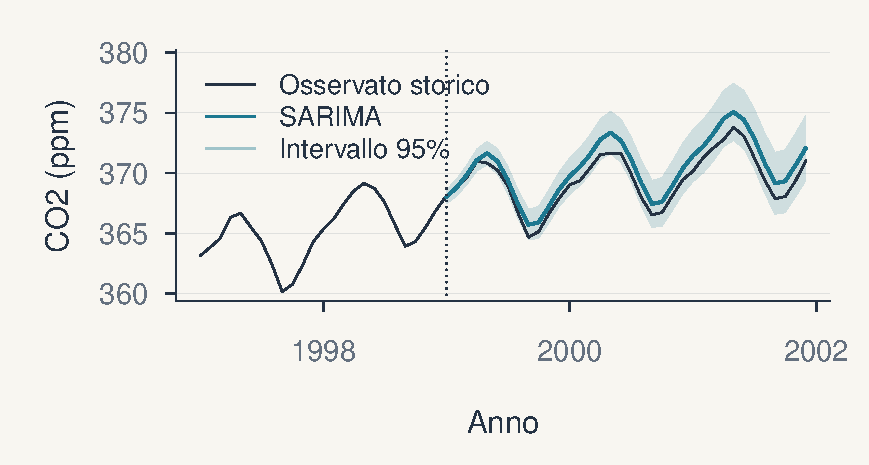
\includegraphics[width=9.85cm,height=5.25cm,keepaspectratio]{Risultati/Figure/03_previsione_CO2.pdf}
\vspace{1.5mm}
\PSmall{Previsione emessa a dicembre 1998; banda puntuale al 95\% condizionata al modello stimato.}

\end{minipage}\end{lrbox}
\typeout{FULLBOX:087:PilotLeftBox:\the\ht\PilotLeftBox:\the\dp\PilotLeftBox}

\begin{lrbox}{\PilotRightBox}
\begin{minipage}[t]{7.55cm}\raggedright\color{Ink}\fontsize{11.3}{14.8}\selectfont
\PBody{Il centro conserva la stagione e prolunga la dinamica del livello. L’intervallo cresce perché aumenta l’incertezza sugli shock futuri.}
\vspace{2.5mm}
\PInfo{I valori osservati sono aggiunti soltanto per valutare la previsione storica. Non entrano nel modello che ha prodotto questa traiettoria.}
\PBody{L’ampiezza della banda va letta insieme all’errore del centro: contengono informazioni complementari.}
\vspace{2.5mm}

\end{minipage}\end{lrbox}
\typeout{FULLBOX:087:PilotRightBox:\the\ht\PilotRightBox:\the\dp\PilotRightBox}

\begin{tikzpicture}[remember picture,overlay]
\PilotChrome{La traiettoria prevista va letta con il suo intervallo}{VII · ERRORI E INTERVALLI}{87}{Un grafico previsionale deve rendere visibili origine, unità, osservazioni e natura della banda.}
\node[anchor=north west,inner sep=0] at([xshift=.96cm,yshift=-2.13cm]current page.north west){\usebox{\PilotLeftBox}};
\node[anchor=north west,inner sep=0] at([xshift=11.52cm,yshift=-2.13cm]current page.north west){\usebox{\PilotRightBox}};
\node[anchor=north east,inner sep=0] at([xshift=17.65cm,yshift=-12.06cm]current page.north west){\color{Classical}\fontsize{7.7}{9.2}\selectfont\href{../../03_Notebook_svolti/M10_Futura/M10_N06.html}{M10\_N06 · notebook svolto}};
\end{tikzpicture}\end{frame}

\begin{frame}[plain]\hypertarget{slide88}{}
\bookmark[level=1,page=88]{L’intervallo gaussiano usa l’errore standard futuro}
\begin{lrbox}{\TitleBox}
\begin{minipage}[t]{17.7cm}\raggedright\color{Ink}\fontsize{11.3}{14.8}\selectfont
\color{Navy}\bfseries\fontsize{20.6}{24.5}\selectfont L’intervallo gaussiano usa l’errore standard futuro
\end{minipage}\end{lrbox}
\typeout{FULLBOX:088:TitleBox:\the\ht\TitleBox:\the\dp\TitleBox}

\begin{lrbox}{\RecallBox}
\begin{minipage}[t]{14.3cm}\raggedright\color{Ink}\fontsize{11.3}{14.8}\selectfont
\fontsize{10.3}{13.8}\selectfont Un intervallo predittivo combina una previsione centrale, una varianza e un’ipotesi distributiva.
\end{minipage}\end{lrbox}
\typeout{FULLBOX:088:RecallBox:\the\ht\RecallBox:\the\dp\RecallBox}

\begin{lrbox}{\PilotLeftBox}
\begin{minipage}[t]{10.05cm}\raggedright\color{Ink}\fontsize{11.3}{14.8}\selectfont
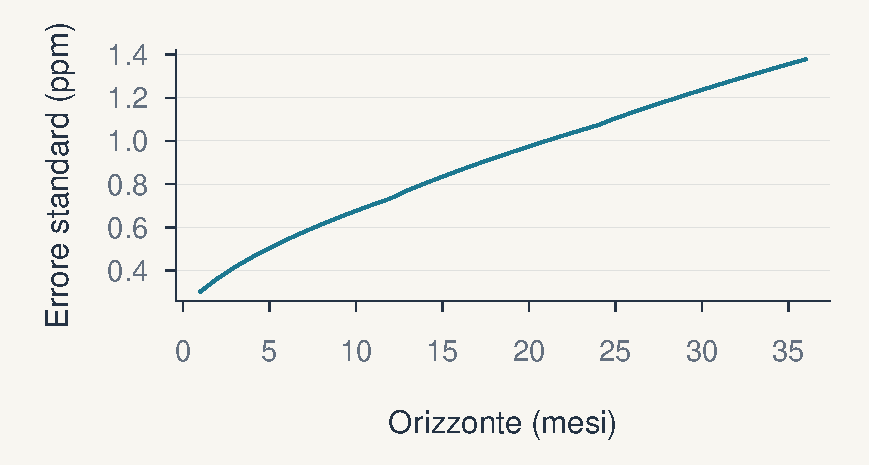
\includegraphics[width=9.85cm,height=5.25cm,keepaspectratio]{Risultati/Figure/11_errore_standard_previsione.pdf}
\vspace{1.5mm}
\PSmall{Errore standard previsto a ogni orizzonte; il modello tratta i parametri stimati come fissati.}
\[I_h=\left[\widehat y_h-z_{0{,}975}s_h,\ \widehat y_h+z_{0{,}975}s_h\right]\]

\end{minipage}\end{lrbox}
\typeout{FULLBOX:088:PilotLeftBox:\the\ht\PilotLeftBox:\the\dp\PilotLeftBox}

\begin{lrbox}{\PilotRightBox}
\begin{minipage}[t]{7.55cm}\raggedright\color{Ink}\fontsize{11.3}{14.8}\selectfont
\PBody{La banda al 95\% usa un quantile normale e l’errore standard della previsione. Si interpreta separatamente per ciascun orizzonte.}
\vspace{2.5mm}
\PInfo{L’errore standard non è lo stesso numero della RMSE misurata sui 36 mesi. Il primo deriva dal modello; la seconda dagli errori realizzati.}
\PCode{R · intervallo al 95\%}{088_esempio.R}
\end{minipage}\end{lrbox}
\typeout{FULLBOX:088:PilotRightBox:\the\ht\PilotRightBox:\the\dp\PilotRightBox}

\begin{tikzpicture}[remember picture,overlay]
\PilotChrome{L’intervallo gaussiano usa l’errore standard futuro}{VII · ERRORI E INTERVALLI}{88}{Un intervallo predittivo combina una previsione centrale, una varianza e un’ipotesi distributiva.}
\node[anchor=north west,inner sep=0] at([xshift=.96cm,yshift=-2.13cm]current page.north west){\usebox{\PilotLeftBox}};
\node[anchor=north west,inner sep=0] at([xshift=11.52cm,yshift=-2.13cm]current page.north west){\usebox{\PilotRightBox}};
\node[anchor=north east,inner sep=0] at([xshift=17.65cm,yshift=-12.06cm]current page.north west){\color{Classical}\fontsize{7.7}{9.2}\selectfont\href{../../03_Notebook_svolti/M10_Futura/M10_N06.html}{M10\_N06 · notebook svolto}};
\end{tikzpicture}\end{frame}

\begin{frame}[plain]\hypertarget{slide89}{}
\bookmark[level=1,page=89]{La banda è condizionata a ipotesi precise}
\begin{lrbox}{\TitleBox}
\begin{minipage}[t]{17.7cm}\raggedright\color{Ink}\fontsize{11.3}{14.8}\selectfont
\color{Navy}\bfseries\fontsize{20.6}{24.5}\selectfont La banda è condizionata a ipotesi precise
\end{minipage}\end{lrbox}
\typeout{FULLBOX:089:TitleBox:\the\ht\TitleBox:\the\dp\TitleBox}

\begin{lrbox}{\RecallBox}
\begin{minipage}[t]{14.3cm}\raggedright\color{Ink}\fontsize{11.3}{14.8}\selectfont
\fontsize{10.3}{13.8}\selectfont Un intervallo va accompagnato da ciò che la sua procedura include e da ciò che lascia fuori.
\end{minipage}\end{lrbox}
\typeout{FULLBOX:089:RecallBox:\the\ht\RecallBox:\the\dp\RecallBox}

\begin{lrbox}{\PilotLeftBox}
\begin{minipage}[t]{10.05cm}\raggedright\color{Ink}\fontsize{11.3}{14.8}\selectfont
{\fontsize{10.2}{13.1}\selectfont\renewcommand{\arraystretch}{1.45}\begin{tabular}{@{}p{4.5cm}p{4.6cm}@{}}\toprule
\textbf{Incluso nel calcolo} & \textbf{Non propagato automaticamente}\\\midrule
Shock futuri del modello & Incertezza dei coefficienti stimati\\
Stato e dinamica stimati & Incertezza nella scelta della famiglia\\
Orizzonte e stagionalità & Cambiamenti strutturali futuri\\
Distribuzione gaussiana assunta & Errori di misura o covariate ignote non modellati\\
\bottomrule\end{tabular}}

\end{minipage}\end{lrbox}
\typeout{FULLBOX:089:PilotLeftBox:\the\ht\PilotLeftBox:\the\dp\PilotLeftBox}

\begin{lrbox}{\PilotRightBox}
\begin{minipage}[t]{7.55cm}\raggedright\color{Ink}\fontsize{11.3}{14.8}\selectfont
\PBody{La documentazione di predict.Arima specifica che gli errori standard escludono l’incertezza dei parametri ARMA e di regressione.}
\vspace{2.5mm}
\PInfo{La banda riguarda il modello stimato e le sue assunzioni. Una copertura nominale non è una promessa incondizionata sul mondo reale.}

\end{minipage}\end{lrbox}
\typeout{FULLBOX:089:PilotRightBox:\the\ht\PilotRightBox:\the\dp\PilotRightBox}

\begin{tikzpicture}[remember picture,overlay]
\PilotChrome{La banda è condizionata a ipotesi precise}{VII · ERRORI E INTERVALLI}{89}{Un intervallo va accompagnato da ciò che la sua procedura include e da ciò che lascia fuori.}
\node[anchor=north west,inner sep=0] at([xshift=.96cm,yshift=-2.13cm]current page.north west){\usebox{\PilotLeftBox}};
\node[anchor=north west,inner sep=0] at([xshift=11.52cm,yshift=-2.13cm]current page.north west){\usebox{\PilotRightBox}};
\end{tikzpicture}\end{frame}

\begin{frame}[plain]\hypertarget{slide90}{}
\bookmark[level=1,page=90]{Valutare copertura e ampiezza insieme}
\begin{lrbox}{\TitleBox}
\begin{minipage}[t]{17.7cm}\raggedright\color{Ink}\fontsize{11.3}{14.8}\selectfont
\color{Navy}\bfseries\fontsize{20.6}{24.5}\selectfont Valutare copertura e ampiezza insieme
\end{minipage}\end{lrbox}
\typeout{FULLBOX:090:TitleBox:\the\ht\TitleBox:\the\dp\TitleBox}

\begin{lrbox}{\RecallBox}
\begin{minipage}[t]{14.3cm}\raggedright\color{Ink}\fontsize{11.3}{14.8}\selectfont
\fontsize{10.3}{13.8}\selectfont Una previsione probabilistica utile deve essere valutata per affidabilità e precisione.
\end{minipage}\end{lrbox}
\typeout{FULLBOX:090:RecallBox:\the\ht\RecallBox:\the\dp\RecallBox}

\begin{lrbox}{\PilotLeftBox}
\begin{minipage}[t]{10.05cm}\raggedright\color{Ink}\fontsize{11.3}{14.8}\selectfont
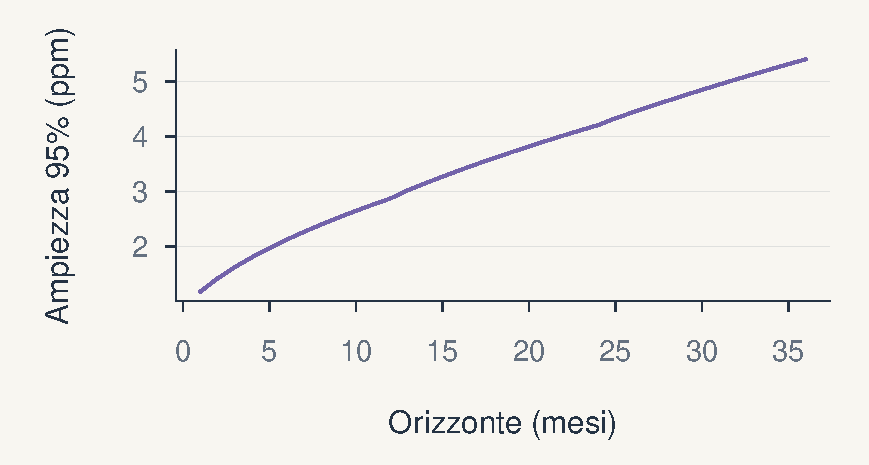
\includegraphics[width=9.85cm,height=5.25cm,keepaspectratio]{Risultati/Figure/13_ampiezza_intervalli.pdf}
\vspace{1.5mm}
\PSmall{Ampiezza degli intervalli puntuali al 95\% per i 36 orizzonti.}
\[A_h=U_h-L_h\]

\end{minipage}\end{lrbox}
\typeout{FULLBOX:090:PilotLeftBox:\the\ht\PilotLeftBox:\the\dp\PilotLeftBox}

\begin{lrbox}{\PilotRightBox}
\begin{minipage}[t]{7.55cm}\raggedright\color{Ink}\fontsize{11.3}{14.8}\selectfont
\PBody{Intervalli molto ampi possono includere molte osservazioni e offrire poca precisione. Una copertura elevata, da sola, non stabilisce l’utilità della previsione.}
\vspace{2.5mm}
\PInfo{Il confronto tra bande richiede lo stesso livello nominale e lo stesso compito. L’ampiezza si interpreta nella scala fisica della variabile.}
\PCode{R · ampiezza delle bande}{090_esempio.R}
\end{minipage}\end{lrbox}
\typeout{FULLBOX:090:PilotRightBox:\the\ht\PilotRightBox:\the\dp\PilotRightBox}

\begin{tikzpicture}[remember picture,overlay]
\PilotChrome{Valutare copertura e ampiezza insieme}{VII · ERRORI E INTERVALLI}{90}{Una previsione probabilistica utile deve essere valutata per affidabilità e precisione.}
\node[anchor=north west,inner sep=0] at([xshift=.96cm,yshift=-2.13cm]current page.north west){\usebox{\PilotLeftBox}};
\node[anchor=north west,inner sep=0] at([xshift=11.52cm,yshift=-2.13cm]current page.north west){\usebox{\PilotRightBox}};
\node[anchor=north east,inner sep=0] at([xshift=17.65cm,yshift=-12.06cm]current page.north west){\color{Classical}\fontsize{7.7}{9.2}\selectfont\href{../../03_Notebook_svolti/M10_Futura/M10_N08.html}{M10\_N08 · notebook svolto}};
\end{tikzpicture}\end{frame}

\begin{frame}[plain]\hypertarget{slide91}{}
\bookmark[level=1,page=91]{Copertura su più traiettorie simulate}
\begin{lrbox}{\TitleBox}
\begin{minipage}[t]{17.7cm}\raggedright\color{Ink}\fontsize{11.3}{14.8}\selectfont
\color{Navy}\bfseries\fontsize{20.6}{24.5}\selectfont Copertura su più traiettorie simulate
\end{minipage}\end{lrbox}
\typeout{FULLBOX:091:TitleBox:\the\ht\TitleBox:\the\dp\TitleBox}

\begin{lrbox}{\RecallBox}
\begin{minipage}[t]{14.3cm}\raggedright\color{Ink}\fontsize{11.3}{14.8}\selectfont
\fontsize{10.3}{13.8}\selectfont La copertura nominale si riferisce a ripetizioni del procedimento nelle condizioni del modello.
\end{minipage}\end{lrbox}
\typeout{FULLBOX:091:RecallBox:\the\ht\RecallBox:\the\dp\RecallBox}

\begin{lrbox}{\PilotLeftBox}
\begin{minipage}[t]{10.05cm}\raggedright\color{Ink}\fontsize{11.3}{14.8}\selectfont
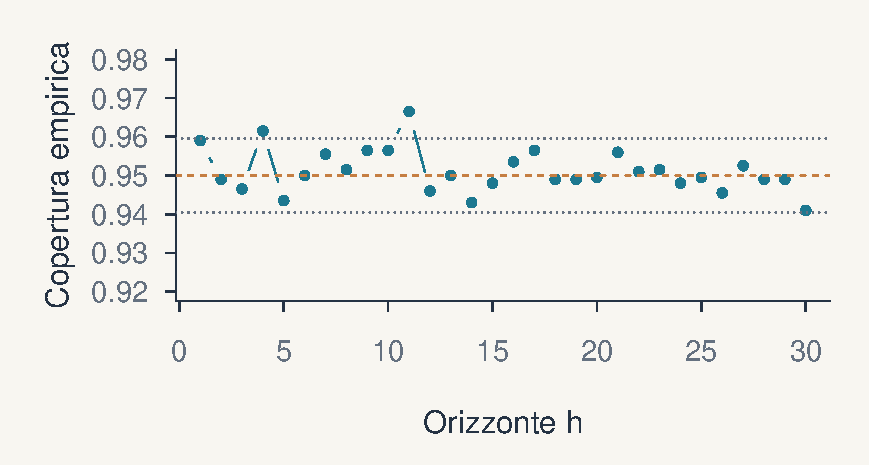
\includegraphics[width=9.85cm,height=5.25cm,keepaspectratio]{Risultati/Figure/23_AR1_copertura_MC.pdf}
\vspace{1.5mm}
\PSmall{2.000 traiettorie AR(1) indipendenti, con parametri noti e identica origine. Copertura per orizzonte.}

\end{minipage}\end{lrbox}
\typeout{FULLBOX:091:PilotLeftBox:\the\ht\PilotLeftBox:\the\dp\PilotLeftBox}

\begin{lrbox}{\PilotRightBox}
\begin{minipage}[t]{7.55cm}\raggedright\color{Ink}\fontsize{11.3}{14.8}\selectfont
\PBody{Nella simulazione conosciamo il processo che genera i dati. Ripetiamo lo stesso esperimento molte volte e contiamo quante osservazioni entrano nell’intervallo a ciascun orizzonte.}
\vspace{2.5mm}
\PInfo{Le repliche indipendenti sono le 2.000 traiettorie. Gli orizzonti della stessa traiettoria rimangono dipendenti.}
\PSmall{Le oscillazioni attorno a 0,95 sono variabilità Monte Carlo: non una correzione applicata alla CO$_2$.}

\end{minipage}\end{lrbox}
\typeout{FULLBOX:091:PilotRightBox:\the\ht\PilotRightBox:\the\dp\PilotRightBox}

\begin{tikzpicture}[remember picture,overlay]
\PilotChrome{Copertura su più traiettorie simulate}{VII · ERRORI E INTERVALLI}{91}{La copertura nominale si riferisce a ripetizioni del procedimento nelle condizioni del modello.}
\node[anchor=north west,inner sep=0] at([xshift=.96cm,yshift=-2.13cm]current page.north west){\usebox{\PilotLeftBox}};
\node[anchor=north west,inner sep=0] at([xshift=11.52cm,yshift=-2.13cm]current page.north west){\usebox{\PilotRightBox}};
\end{tikzpicture}\end{frame}

\begin{frame}[plain]\hypertarget{slide92}{}
\bookmark[level=1,page=92]{Copertura osservata e calibrazione}
\begin{lrbox}{\TitleBox}
\begin{minipage}[t]{17.7cm}\raggedright\color{Ink}\fontsize{11.3}{14.8}\selectfont
\color{Navy}\bfseries\fontsize{20.6}{24.5}\selectfont Copertura osservata e calibrazione
\end{minipage}\end{lrbox}
\typeout{FULLBOX:092:TitleBox:\the\ht\TitleBox:\the\dp\TitleBox}

\begin{lrbox}{\RecallBox}
\begin{minipage}[t]{14.3cm}\raggedright\color{Ink}\fontsize{11.3}{14.8}\selectfont
\fontsize{10.3}{13.8}\selectfont La copertura empirica di una singola traiettoria va descritta senza attribuirle una certezza che non possiede.
\end{minipage}\end{lrbox}
\typeout{FULLBOX:092:RecallBox:\the\ht\RecallBox:\the\dp\RecallBox}

\begin{lrbox}{\PilotLeftBox}
\begin{minipage}[t]{10.05cm}\raggedright\color{Ink}\fontsize{11.3}{14.8}\selectfont
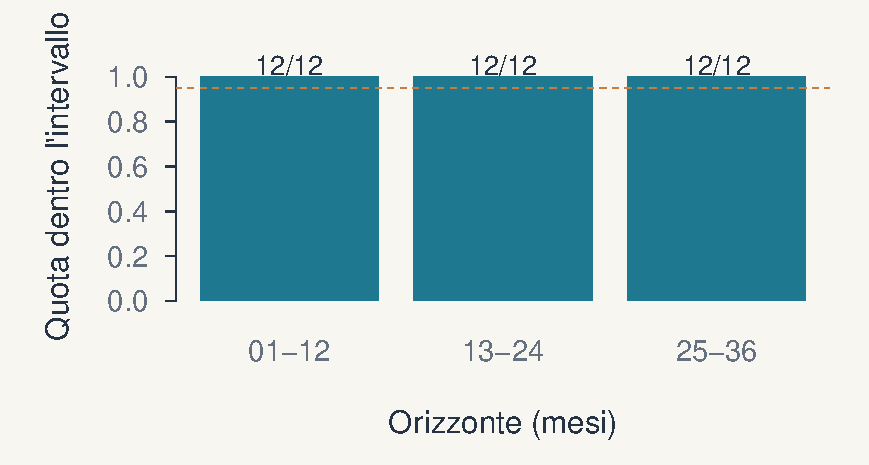
\includegraphics[width=9.85cm,height=4.75cm,keepaspectratio]{Risultati/Figure/12_copertura_blocchi.pdf}
\vspace{1.5mm}
\PSmall{Test storico diviso nei tre blocchi di 12 mesi; tutti i 36 valori risultano inclusi nelle bande.}
\[\widehat C=\frac{1}{36}\sum_{h=1}^{36}\mathbf1\{y_{T+h}\in I_h\}=1\]

\end{minipage}\end{lrbox}
\typeout{FULLBOX:092:PilotLeftBox:\the\ht\PilotLeftBox:\the\dp\PilotLeftBox}

\begin{lrbox}{\PilotRightBox}
\begin{minipage}[t]{7.55cm}\raggedright\color{Ink}\fontsize{11.3}{14.8}\selectfont
\PBody{Il risultato descrittivo è 36 su 36. I punti appartengono a una sola traiettoria con origine comune e non sono 36 prove Bernoulli indipendenti.}
\vspace{2.5mm}
\PInfo{Non ricaviamo da questo conteggio una prova di calibrazione al 95\%, né la probabilità che l’intera traiettoria futura resti nella banda.}
\PSmall{Una banda puntuale al 95\% non è una banda simultanea al 95\% per tutti gli orizzonti.}

\end{minipage}\end{lrbox}
\typeout{FULLBOX:092:PilotRightBox:\the\ht\PilotRightBox:\the\dp\PilotRightBox}

\begin{tikzpicture}[remember picture,overlay]
\PilotChrome{Copertura osservata e calibrazione}{VII · ERRORI E INTERVALLI}{92}{La copertura empirica di una singola traiettoria va descritta senza attribuirle una certezza che non possiede.}
\node[anchor=north west,inner sep=0] at([xshift=.96cm,yshift=-2.13cm]current page.north west){\usebox{\PilotLeftBox}};
\node[anchor=north west,inner sep=0] at([xshift=11.52cm,yshift=-2.13cm]current page.north west){\usebox{\PilotRightBox}};
\node[anchor=north east,inner sep=0] at([xshift=17.65cm,yshift=-12.06cm]current page.north west){\color{Classical}\fontsize{7.7}{9.2}\selectfont\href{../../03_Notebook_svolti/M10_Futura/M10_N08.html}{M10\_N08 · notebook svolto}};
\end{tikzpicture}\end{frame}

\begin{frame}[plain]\hypertarget{slide93}{}
\bookmark[level=1,page=93]{La verifica teorica aiuta a controllare i calcoli}
\begin{lrbox}{\TitleBox}
\begin{minipage}[t]{17.7cm}\raggedright\color{Ink}\fontsize{11.3}{14.8}\selectfont
\color{Navy}\bfseries\fontsize{20.6}{24.5}\selectfont La verifica teorica aiuta a controllare i calcoli
\end{minipage}\end{lrbox}
\typeout{FULLBOX:093:TitleBox:\the\ht\TitleBox:\the\dp\TitleBox}

\begin{lrbox}{\RecallBox}
\begin{minipage}[t]{14.3cm}\raggedright\color{Ink}\fontsize{11.3}{14.8}\selectfont
\fontsize{10.3}{13.8}\selectfont Un caso teorico noto è un controllo utile dei calcoli e ha un ambito di validità esplicito.
\end{minipage}\end{lrbox}
\typeout{FULLBOX:093:RecallBox:\the\ht\RecallBox:\the\dp\RecallBox}

\begin{lrbox}{\PilotLeftBox}
\begin{minipage}[t]{10.05cm}\raggedright\color{Ink}\fontsize{11.3}{14.8}\selectfont
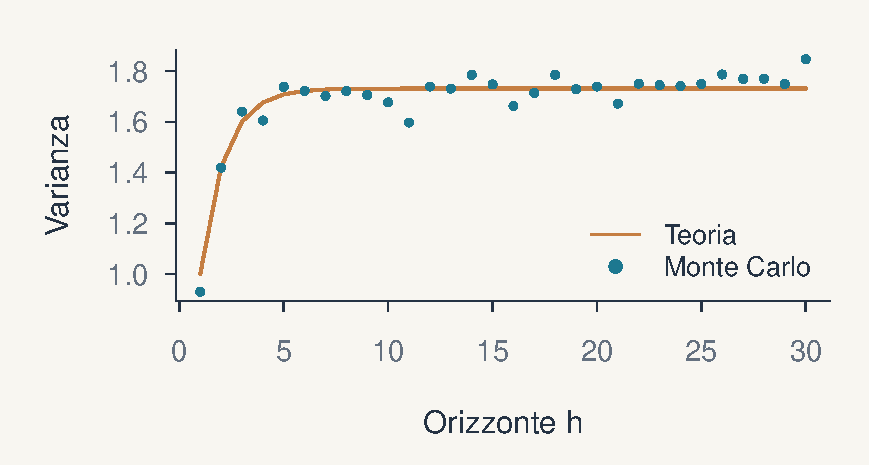
\includegraphics[width=9.85cm,height=5.25cm,keepaspectratio]{Risultati/Figure/24_AR1_varianza_MC.pdf}
\vspace{1.5mm}
\PSmall{Varianza empirica su 2.000 repliche confrontata con la formula AR(1) a parametri noti.}

\end{minipage}\end{lrbox}
\typeout{FULLBOX:093:PilotLeftBox:\the\ht\PilotLeftBox:\the\dp\PilotLeftBox}

\begin{lrbox}{\PilotRightBox}
\begin{minipage}[t]{7.55cm}\raggedright\color{Ink}\fontsize{11.3}{14.8}\selectfont
\PBody{Nel caso simulato la formula della varianza è nota. La concordanza con il calcolo Monte Carlo controlla la ricorsione, i pesi e l’orientamento degli indici.}
\vspace{2.5mm}
\PInfo{Questo controllo valida un’implementazione in un caso noto. Non dimostra che il SARIMA descriva perfettamente la serie storica di CO$_2$.}
\PBody{La verifica numerica e la validità scientifica hanno entrambe un ruolo, ma rispondono a domande distinte.}
\vspace{2.5mm}

\end{minipage}\end{lrbox}
\typeout{FULLBOX:093:PilotRightBox:\the\ht\PilotRightBox:\the\dp\PilotRightBox}

\begin{tikzpicture}[remember picture,overlay]
\PilotChrome{La verifica teorica aiuta a controllare i calcoli}{VII · ERRORI E INTERVALLI}{93}{Un caso teorico noto è un controllo utile dei calcoli e ha un ambito di validità esplicito.}
\node[anchor=north west,inner sep=0] at([xshift=.96cm,yshift=-2.13cm]current page.north west){\usebox{\PilotLeftBox}};
\node[anchor=north west,inner sep=0] at([xshift=11.52cm,yshift=-2.13cm]current page.north west){\usebox{\PilotRightBox}};
\end{tikzpicture}\end{frame}

\begin{frame}[plain]\hypertarget{slide94}{}
\bookmark[level=0,page=94]{VIII · SISTEMI MULTIVARIATI}
\bookmark[level=1,page=94]{Un VAR collega i passati di due variabili}
\begin{lrbox}{\TitleBox}
\begin{minipage}[t]{17.7cm}\raggedright\color{Ink}\fontsize{11.3}{14.8}\selectfont
\color{Navy}\bfseries\fontsize{20.6}{24.5}\selectfont Un VAR collega i passati di due variabili
\end{minipage}\end{lrbox}
\typeout{FULLBOX:094:TitleBox:\the\ht\TitleBox:\the\dp\TitleBox}

\begin{lrbox}{\RecallBox}
\begin{minipage}[t]{14.3cm}\raggedright\color{Ink}\fontsize{11.3}{14.8}\selectfont
\fontsize{10.3}{13.8}\selectfont Un modello multivariato valuta se il passato congiunto aggiunge informazione previsionale.
\end{minipage}\end{lrbox}
\typeout{FULLBOX:094:RecallBox:\the\ht\RecallBox:\the\dp\RecallBox}

\begin{lrbox}{\PilotLeftBox}
\begin{minipage}[t]{10.05cm}\raggedright\color{Ink}\fontsize{11.3}{14.8}\selectfont
\begin{tikzpicture}[x=1cm,y=1cm]
\path[use as bounding box](-.1,-.15) rectangle(9.7,4.6);
\node[pFlow,text width=2.8cm,fill=GeoA!8](xp)at(2,3.6){$X_{t-1}$};
\node[pFlow,text width=2.8cm,fill=GeoB!8](yp)at(2,1.1){$Y_{t-1}$};
\node[pFlow,text width=2.8cm,fill=GeoA!8](x)at(7.6,3.6){$X_t$};
\node[pFlow,text width=2.8cm,fill=GeoB!8](y)at(7.6,1.1){$Y_t$};
\draw[pEdge](xp)--node[above,pNote]{$a_{11}$}(x);
\draw[pEdge](yp)--node[below,pNote]{$a_{22}$}(y);
\draw[pEdge,GeoC](xp)--node[pos=.25,below,pNote]{$a_{21}$}(y);
\draw[pEdge,GeoC](yp)--node[pos=.25,above,pNote]{$a_{12}$}(x);
\end{tikzpicture}
\[\mathbf Z_t=\mathbf c+A\mathbf Z_{t-1}+\boldsymbol\varepsilon_t\]

\end{minipage}\end{lrbox}
\typeout{FULLBOX:094:PilotLeftBox:\the\ht\PilotLeftBox:\the\dp\PilotLeftBox}

\begin{lrbox}{\PilotRightBox}
\begin{minipage}[t]{7.55cm}\raggedright\color{Ink}\fontsize{11.3}{14.8}\selectfont
\PBody{Ogni equazione usa il valore passato della variabile stessa e quello dell’altra. I coefficienti incrociati descrivono un contributo predittivo condizionato al modello.}
\vspace{2.5mm}
\PInfo{Il laboratorio usa x\_VAR e y\_VAR di un archivio simulato. I primi 250 tempi servono alla stima, i successivi 10 alla verifica.}
\PCode{R · due equazioni collegate}{094_esempio.R}
\end{minipage}\end{lrbox}
\typeout{FULLBOX:094:PilotRightBox:\the\ht\PilotRightBox:\the\dp\PilotRightBox}

\begin{tikzpicture}[remember picture,overlay]
\PilotChrome{Un VAR collega i passati di due variabili}{VIII · SISTEMI MULTIVARIATI}{94}{Un modello multivariato valuta se il passato congiunto aggiunge informazione previsionale.}
\node[anchor=north west,inner sep=0] at([xshift=.96cm,yshift=-2.13cm]current page.north west){\usebox{\PilotLeftBox}};
\node[anchor=north west,inner sep=0] at([xshift=11.52cm,yshift=-2.13cm]current page.north west){\usebox{\PilotRightBox}};
\node[anchor=north east,inner sep=0] at([xshift=17.65cm,yshift=-12.06cm]current page.north west){\color{Classical}\fontsize{7.7}{9.2}\selectfont\href{../../03_Notebook_svolti/M10_Futura/M10_N14.html}{M10\_N14 · notebook svolto}};
\end{tikzpicture}\end{frame}

\begin{frame}[plain]\hypertarget{slide95}{}
\bookmark[level=1,page=95]{Le due regressioni condividono le stesse righe}
\begin{lrbox}{\TitleBox}
\begin{minipage}[t]{17.7cm}\raggedright\color{Ink}\fontsize{11.3}{14.8}\selectfont
\color{Navy}\bfseries\fontsize{20.6}{24.5}\selectfont Le due regressioni condividono le stesse righe
\end{minipage}\end{lrbox}
\typeout{FULLBOX:095:TitleBox:\the\ht\TitleBox:\the\dp\TitleBox}

\begin{lrbox}{\RecallBox}
\begin{minipage}[t]{14.3cm}\raggedright\color{Ink}\fontsize{11.3}{14.8}\selectfont
\fontsize{10.3}{13.8}\selectfont Una regressione con ritardi deve conservare il significato temporale di ogni coppia.
\end{minipage}\end{lrbox}
\typeout{FULLBOX:095:RecallBox:\the\ht\RecallBox:\the\dp\RecallBox}

\begin{lrbox}{\PilotLeftBox}
\begin{minipage}[t]{10.05cm}\raggedright\color{Ink}\fontsize{11.3}{14.8}\selectfont
\[X_t=c_x+a_{11}X_{t-1}+a_{12}Y_{t-1}+\varepsilon_{x,t}\]
\[Y_t=c_y+a_{21}X_{t-1}+a_{22}Y_{t-1}+\varepsilon_{y,t}\]
{\fontsize{10.2}{13.1}\selectfont\renewcommand{\arraystretch}{1.45}\begin{tabular}{@{}p{4.5cm}p{4.6cm}@{}}\toprule
\textbf{Risposte} & \textbf{Regressori}\\\midrule
Tempi 2--250 & Tempi 1--249\\
249 coppie complete & Stessa matrice per entrambe le equazioni\\
\bottomrule\end{tabular}}

\end{minipage}\end{lrbox}
\typeout{FULLBOX:095:PilotLeftBox:\the\ht\PilotLeftBox:\the\dp\PilotLeftBox}

\begin{lrbox}{\PilotRightBox}
\begin{minipage}[t]{7.55cm}\raggedright\color{Ink}\fontsize{11.3}{14.8}\selectfont
\PBody{Il ritardo si costruisce mantenendo l’allineamento. Eliminare valori mancanti separatamente nelle due serie potrebbe produrre coppie temporali scorrette.}
\vspace{2.5mm}
\PInfo{Nel dataset del laboratorio le righe usate sono complete. Con lo stesso insieme di regressori, si possono stimare le due equazioni separatamente con lm.}
\PCode{R · equazioni sulle stesse coppie}{095_esempio.R}
\end{minipage}\end{lrbox}
\typeout{FULLBOX:095:PilotRightBox:\the\ht\PilotRightBox:\the\dp\PilotRightBox}

\begin{tikzpicture}[remember picture,overlay]
\PilotChrome{Le due regressioni condividono le stesse righe}{VIII · SISTEMI MULTIVARIATI}{95}{Una regressione con ritardi deve conservare il significato temporale di ogni coppia.}
\node[anchor=north west,inner sep=0] at([xshift=.96cm,yshift=-2.13cm]current page.north west){\usebox{\PilotLeftBox}};
\node[anchor=north west,inner sep=0] at([xshift=11.52cm,yshift=-2.13cm]current page.north west){\usebox{\PilotRightBox}};
\node[anchor=north east,inner sep=0] at([xshift=17.65cm,yshift=-12.06cm]current page.north west){\color{Classical}\fontsize{7.7}{9.2}\selectfont\href{../../03_Notebook_svolti/M10_Futura/M10_N14.html}{M10\_N14 · notebook svolto}};
\end{tikzpicture}\end{frame}

\begin{frame}[plain]\hypertarget{slide96}{}
\bookmark[level=1,page=96]{La stabilità VAR riguarda gli autovalori della matrice}
\begin{lrbox}{\TitleBox}
\begin{minipage}[t]{17.7cm}\raggedright\color{Ink}\fontsize{11.3}{14.8}\selectfont
\color{Navy}\bfseries\fontsize{20.6}{24.5}\selectfont La stabilità VAR riguarda gli autovalori della matrice
\end{minipage}\end{lrbox}
\typeout{FULLBOX:096:TitleBox:\the\ht\TitleBox:\the\dp\TitleBox}

\begin{lrbox}{\RecallBox}
\begin{minipage}[t]{14.3cm}\raggedright\color{Ink}\fontsize{11.3}{14.8}\selectfont
\fontsize{10.3}{13.8}\selectfont La stabilità VAR si controlla sugli autovalori della matrice, distinguendoli dalle radici del polinomio AR.
\end{minipage}\end{lrbox}
\typeout{FULLBOX:096:RecallBox:\the\ht\RecallBox:\the\dp\RecallBox}

\begin{lrbox}{\PilotLeftBox}
\begin{minipage}[t]{10.05cm}\raggedright\color{Ink}\fontsize{11.3}{14.8}\selectfont
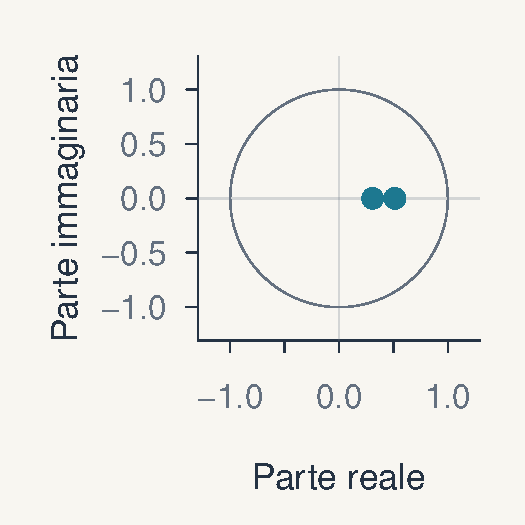
\includegraphics[width=9.85cm,height=5.25cm,keepaspectratio]{Risultati/Figure/31_VAR_autovalori.pdf}
\vspace{1.5mm}
\PSmall{Autovalori della matrice VAR(1) stimata rispetto al cerchio unitario.}
\[\rho(A)=\max_j|\lambda_j|=0,514<1\]

\end{minipage}\end{lrbox}
\typeout{FULLBOX:096:PilotLeftBox:\the\ht\PilotLeftBox:\the\dp\PilotLeftBox}

\begin{lrbox}{\PilotRightBox}
\begin{minipage}[t]{7.55cm}\raggedright\color{Ink}\fontsize{11.3}{14.8}\selectfont
\PBody{Per un VAR(1) stabile, le potenze di A si attenuano. Gli autovalori della matrice dinamica devono stare dentro il cerchio unitario.}
\vspace{2.5mm}
\PInfo{Per l’AR avevamo chiesto radici del polinomio fuori dal cerchio. Non è una contraddizione: le due convenzioni sono reciproche.}
\PCode{R · raggio spettrale}{096_esempio.R}
\end{minipage}\end{lrbox}
\typeout{FULLBOX:096:PilotRightBox:\the\ht\PilotRightBox:\the\dp\PilotRightBox}

\begin{tikzpicture}[remember picture,overlay]
\PilotChrome{La stabilità VAR riguarda gli autovalori della matrice}{VIII · SISTEMI MULTIVARIATI}{96}{La stabilità VAR si controlla sugli autovalori della matrice, distinguendoli dalle radici del polinomio AR.}
\node[anchor=north west,inner sep=0] at([xshift=.96cm,yshift=-2.13cm]current page.north west){\usebox{\PilotLeftBox}};
\node[anchor=north west,inner sep=0] at([xshift=11.52cm,yshift=-2.13cm]current page.north west){\usebox{\PilotRightBox}};
\node[anchor=north east,inner sep=0] at([xshift=17.65cm,yshift=-12.06cm]current page.north west){\color{Classical}\fontsize{7.7}{9.2}\selectfont\href{../../03_Notebook_svolti/M10_Futura/M10_N15.html}{M10\_N15 · notebook svolto}};
\end{tikzpicture}\end{frame}

\begin{frame}[plain]\hypertarget{slide97}{}
\bookmark[level=1,page=97]{Le equazioni multivariate richiedono diagnostica}
\begin{lrbox}{\TitleBox}
\begin{minipage}[t]{17.7cm}\raggedright\color{Ink}\fontsize{11.3}{14.8}\selectfont
\color{Navy}\bfseries\fontsize{20.6}{24.5}\selectfont Le equazioni multivariate richiedono diagnostica
\end{minipage}\end{lrbox}
\typeout{FULLBOX:097:TitleBox:\the\ht\TitleBox:\the\dp\TitleBox}

\begin{lrbox}{\RecallBox}
\begin{minipage}[t]{14.3cm}\raggedright\color{Ink}\fontsize{11.3}{14.8}\selectfont
\fontsize{10.3}{13.8}\selectfont Passare a due variabili amplia anche le strutture residue che devono essere controllate.
\end{minipage}\end{lrbox}
\typeout{FULLBOX:097:RecallBox:\the\ht\RecallBox:\the\dp\RecallBox}

\begin{lrbox}{\PilotLeftBox}
\begin{minipage}[t]{10.05cm}\raggedright\color{Ink}\fontsize{11.3}{14.8}\selectfont
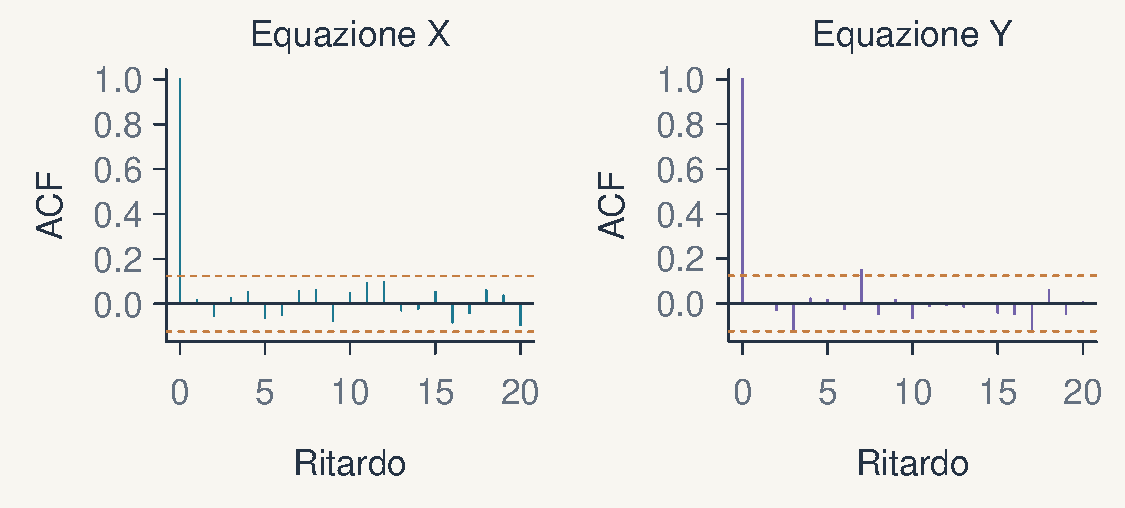
\includegraphics[width=9.85cm,height=5.25cm,keepaspectratio]{Risultati/Figure/33_VAR_ACF_residui.pdf}
\vspace{1.5mm}
\PSmall{ACF dei residui delle due equazioni, stimati sui primi 250 tempi.}

\end{minipage}\end{lrbox}
\typeout{FULLBOX:097:PilotLeftBox:\the\ht\PilotLeftBox:\the\dp\PilotLeftBox}

\begin{lrbox}{\PilotRightBox}
\begin{minipage}[t]{7.55cm}\raggedright\color{Ink}\fontsize{11.3}{14.8}\selectfont
\PBody{Per ogni equazione si esaminano sequenza, dispersione e autocorrelazione residua. In un sistema multivariato possono restare anche dipendenze incrociate.}
\vspace{2.5mm}
\PInfo{Le due ACF marginali sono un primo controllo. Non costituiscono da sole una diagnostica multivariata completa né un test di indipendenza congiunta.}
\PSmall{L’esempio resta una base didattica: rende verificabili allineamento, stabilità e contributo del ritardo dell’altra variabile.}

\end{minipage}\end{lrbox}
\typeout{FULLBOX:097:PilotRightBox:\the\ht\PilotRightBox:\the\dp\PilotRightBox}

\begin{tikzpicture}[remember picture,overlay]
\PilotChrome{Le equazioni multivariate richiedono diagnostica}{VIII · SISTEMI MULTIVARIATI}{97}{Passare a due variabili amplia anche le strutture residue che devono essere controllate.}
\node[anchor=north west,inner sep=0] at([xshift=.96cm,yshift=-2.13cm]current page.north west){\usebox{\PilotLeftBox}};
\node[anchor=north west,inner sep=0] at([xshift=11.52cm,yshift=-2.13cm]current page.north west){\usebox{\PilotRightBox}};
\node[anchor=north east,inner sep=0] at([xshift=17.65cm,yshift=-12.06cm]current page.north west){\color{Classical}\fontsize{7.7}{9.2}\selectfont\href{../../03_Notebook_svolti/M10_Futura/M10_N15.html}{M10\_N15 · notebook svolto}};
\end{tikzpicture}\end{frame}

\begin{frame}[plain]\hypertarget{slide98}{}
\bookmark[level=1,page=98]{Granger confronta due modelli annidati}
\begin{lrbox}{\TitleBox}
\begin{minipage}[t]{17.7cm}\raggedright\color{Ink}\fontsize{11.3}{14.8}\selectfont
\color{Navy}\bfseries\fontsize{20.6}{24.5}\selectfont Granger confronta due modelli annidati
\end{minipage}\end{lrbox}
\typeout{FULLBOX:098:TitleBox:\the\ht\TitleBox:\the\dp\TitleBox}

\begin{lrbox}{\RecallBox}
\begin{minipage}[t]{14.3cm}\raggedright\color{Ink}\fontsize{11.3}{14.8}\selectfont
\fontsize{10.3}{13.8}\selectfont Il risultato di Granger è condizionato a variabili, ritardi, periodo e ipotesi del modello.
\end{minipage}\end{lrbox}
\typeout{FULLBOX:098:RecallBox:\the\ht\RecallBox:\the\dp\RecallBox}

\begin{lrbox}{\PilotLeftBox}
\begin{minipage}[t]{10.05cm}\raggedright\color{Ink}\fontsize{11.3}{14.8}\selectfont
\PLabel{Il passato di X aggiunge informazione per Y?}
\[M_R:\ Y_t=c+aY_{t-1}+u_t\]
\[M_F:\ Y_t=c+aY_{t-1}+bX_{t-1}+u_t\]
\[H_0:b=0\]

\end{minipage}\end{lrbox}
\typeout{FULLBOX:098:PilotLeftBox:\the\ht\PilotLeftBox:\the\dp\PilotLeftBox}

\begin{lrbox}{\PilotRightBox}
\begin{minipage}[t]{7.55cm}\raggedright\color{Ink}\fontsize{11.3}{14.8}\selectfont
\PBody{Il modello ridotto usa il solo passato di Y. Quello completo aggiunge il passato di X. Il confronto richiede la stessa risposta e le stesse osservazioni.}
\vspace{2.5mm}
\PInfo{Una significatività indica contributo predittivo nella specifica considerata. Non dimostra causalità fisica né esclude variabili comuni omesse.}
\PCode{R · confronto X verso Y}{098_esempio.R}
\end{minipage}\end{lrbox}
\typeout{FULLBOX:098:PilotRightBox:\the\ht\PilotRightBox:\the\dp\PilotRightBox}

\begin{tikzpicture}[remember picture,overlay]
\PilotChrome{Granger confronta due modelli annidati}{VIII · SISTEMI MULTIVARIATI}{98}{Il risultato di Granger è condizionato a variabili, ritardi, periodo e ipotesi del modello.}
\node[anchor=north west,inner sep=0] at([xshift=.96cm,yshift=-2.13cm]current page.north west){\usebox{\PilotLeftBox}};
\node[anchor=north west,inner sep=0] at([xshift=11.52cm,yshift=-2.13cm]current page.north west){\usebox{\PilotRightBox}};
\node[anchor=north east,inner sep=0] at([xshift=17.65cm,yshift=-12.06cm]current page.north west){\color{Classical}\fontsize{7.7}{9.2}\selectfont\href{../../03_Notebook_svolti/M10_Futura/M10_N16.html}{M10\_N16 · notebook svolto}};
\end{tikzpicture}\end{frame}

\begin{frame}[plain]\hypertarget{slide99}{}
\bookmark[level=1,page=99]{Le due direzioni richiedono una lettura congiunta}
\begin{lrbox}{\TitleBox}
\begin{minipage}[t]{17.7cm}\raggedright\color{Ink}\fontsize{11.3}{14.8}\selectfont
\color{Navy}\bfseries\fontsize{20.6}{24.5}\selectfont Le due direzioni richiedono una lettura congiunta
\end{minipage}\end{lrbox}
\typeout{FULLBOX:099:TitleBox:\the\ht\TitleBox:\the\dp\TitleBox}

\begin{lrbox}{\RecallBox}
\begin{minipage}[t]{14.3cm}\raggedright\color{Ink}\fontsize{11.3}{14.8}\selectfont
\fontsize{10.3}{13.8}\selectfont L’interpretazione scientifica deve restare più specifica dell’etichetta “causalità di Granger”.
\end{minipage}\end{lrbox}
\typeout{FULLBOX:099:RecallBox:\the\ht\RecallBox:\the\dp\RecallBox}

\begin{lrbox}{\PilotLeftBox}
\begin{minipage}[t]{10.05cm}\raggedright\color{Ink}\fontsize{11.3}{14.8}\selectfont
\PLabel{Confronti sui medesimi 249 tempi}
{\fontsize{10.2}{13.1}\selectfont\renewcommand{\arraystretch}{1.45}\begin{tabular}{@{}p{2.0835cm}p{2.0835cm}p{2.0835cm}p{2.0835cm}@{}}\toprule
\textbf{Direzione} & \textbf{F} & \textbf{p} & \textbf{p Holm}\\\midrule
X verso Y & 85,197 & 1,3e-17 & 2,6e-17\\
Y verso X & 0,057 & 0,811 & 0,811\\
\bottomrule\end{tabular}}
\PInfo{La correzione di Holm riguarda la famiglia delle due direzioni esaminate. Le ipotesi dei test F restano necessarie.}

\end{minipage}\end{lrbox}
\typeout{FULLBOX:099:PilotLeftBox:\the\ht\PilotLeftBox:\the\dp\PilotLeftBox}

\begin{lrbox}{\PilotRightBox}
\begin{minipage}[t]{7.55cm}\raggedright\color{Ink}\fontsize{11.3}{14.8}\selectfont
\PBody{Nell’archivio simulato emerge un contributo del passato di X alla previsione di Y, mentre la direzione opposta non presenta evidenza analoga.}
\vspace{2.5mm}
\PInfo{La conclusione riguarda il sistema simulato e il VAR(1). Non attribuisce un effetto causale a una misura ambientale reale.}
\PCode{R · due direzioni, correzione Holm}{099_esempio.R}
\end{minipage}\end{lrbox}
\typeout{FULLBOX:099:PilotRightBox:\the\ht\PilotRightBox:\the\dp\PilotRightBox}

\begin{tikzpicture}[remember picture,overlay]
\PilotChrome{Le due direzioni richiedono una lettura congiunta}{VIII · SISTEMI MULTIVARIATI}{99}{L’interpretazione scientifica deve restare più specifica dell’etichetta “causalità di Granger”.}
\node[anchor=north west,inner sep=0] at([xshift=.96cm,yshift=-2.13cm]current page.north west){\usebox{\PilotLeftBox}};
\node[anchor=north west,inner sep=0] at([xshift=11.52cm,yshift=-2.13cm]current page.north west){\usebox{\PilotRightBox}};
\node[anchor=north east,inner sep=0] at([xshift=17.65cm,yshift=-12.06cm]current page.north west){\color{Classical}\fontsize{7.7}{9.2}\selectfont\href{../../03_Notebook_svolti/M10_Futura/M10_N16.html}{M10\_N16 · notebook svolto}};
\end{tikzpicture}\end{frame}

\begin{frame}[plain]\hypertarget{slide100}{}
\bookmark[level=1,page=100]{La previsione VAR usa i propri valori futuri}
\begin{lrbox}{\TitleBox}
\begin{minipage}[t]{17.7cm}\raggedright\color{Ink}\fontsize{11.3}{14.8}\selectfont
\color{Navy}\bfseries\fontsize{20.6}{24.5}\selectfont La previsione VAR usa i propri valori futuri
\end{minipage}\end{lrbox}
\typeout{FULLBOX:100:TitleBox:\the\ht\TitleBox:\the\dp\TitleBox}

\begin{lrbox}{\RecallBox}
\begin{minipage}[t]{14.3cm}\raggedright\color{Ink}\fontsize{11.3}{14.8}\selectfont
\fontsize{10.3}{13.8}\selectfont La ricorsione multistep deve rispettare l’informazione disponibile all’unica origine dichiarata.
\end{minipage}\end{lrbox}
\typeout{FULLBOX:100:RecallBox:\the\ht\RecallBox:\the\dp\RecallBox}

\begin{lrbox}{\PilotLeftBox}
\begin{minipage}[t]{10.05cm}\raggedright\color{Ink}\fontsize{11.3}{14.8}\selectfont
\[\widehat{\mathbf Z}_{T+1\mid T}=\widehat{\mathbf c}+\widehat A\mathbf Z_T\]
\[\widehat{\mathbf Z}_{T+h\mid T}=\widehat{\mathbf c}+\widehat A\widehat{\mathbf Z}_{T+h-1\mid T}\]
\PInfo{Dopo il primo passo si riusano le previsioni, non le osservazioni future del file.}

\end{minipage}\end{lrbox}
\typeout{FULLBOX:100:PilotLeftBox:\the\ht\PilotLeftBox:\the\dp\PilotLeftBox}

\begin{lrbox}{\PilotRightBox}
\begin{minipage}[t]{7.55cm}\raggedright\color{Ink}\fontsize{11.3}{14.8}\selectfont
\PBody{Una previsione ricorsiva a 10 passi parte dal tempo 250. Usare il vero valore del tempo 251 per prevedere 252 cambierebbe il compito in una sequenza di previsioni aggiornate.}
\vspace{2.5mm}
\PInfo{La risposta a uno shock fissato si propaga come $A^h\mathbf u$. Attribuire agli shock un significato strutturale richiederebbe ulteriori ipotesi.}
\PCode{R · dieci passi ricorsivi}{100_esempio.R}
\end{minipage}\end{lrbox}
\typeout{FULLBOX:100:PilotRightBox:\the\ht\PilotRightBox:\the\dp\PilotRightBox}

\begin{tikzpicture}[remember picture,overlay]
\PilotChrome{La previsione VAR usa i propri valori futuri}{VIII · SISTEMI MULTIVARIATI}{100}{La ricorsione multistep deve rispettare l’informazione disponibile all’unica origine dichiarata.}
\node[anchor=north west,inner sep=0] at([xshift=.96cm,yshift=-2.13cm]current page.north west){\usebox{\PilotLeftBox}};
\node[anchor=north west,inner sep=0] at([xshift=11.52cm,yshift=-2.13cm]current page.north west){\usebox{\PilotRightBox}};
\node[anchor=north east,inner sep=0] at([xshift=17.65cm,yshift=-12.06cm]current page.north west){\color{Classical}\fontsize{7.7}{9.2}\selectfont\href{../../03_Notebook_svolti/M10_Futura/M10_N17.html}{M10\_N17 · notebook svolto}};
\end{tikzpicture}\end{frame}

\begin{frame}[plain]\hypertarget{slide101}{}
\bookmark[level=1,page=101]{Il test VAR conserva due errori e un riferimento}
\begin{lrbox}{\TitleBox}
\begin{minipage}[t]{17.7cm}\raggedright\color{Ink}\fontsize{11.3}{14.8}\selectfont
\color{Navy}\bfseries\fontsize{20.6}{24.5}\selectfont Il test VAR conserva due errori e un riferimento
\end{minipage}\end{lrbox}
\typeout{FULLBOX:101:TitleBox:\the\ht\TitleBox:\the\dp\TitleBox}

\begin{lrbox}{\RecallBox}
\begin{minipage}[t]{14.3cm}\raggedright\color{Ink}\fontsize{11.3}{14.8}\selectfont
\fontsize{10.3}{13.8}\selectfont Un’estensione multivariata deve mostrare il beneficio osservato per ciascuna variabile.
\end{minipage}\end{lrbox}
\typeout{FULLBOX:101:RecallBox:\the\ht\RecallBox:\the\dp\RecallBox}

\begin{lrbox}{\FullWideBox}
\begin{minipage}[t]{18.1cm}\raggedright\color{Ink}\fontsize{11.3}{14.8}\selectfont
\centering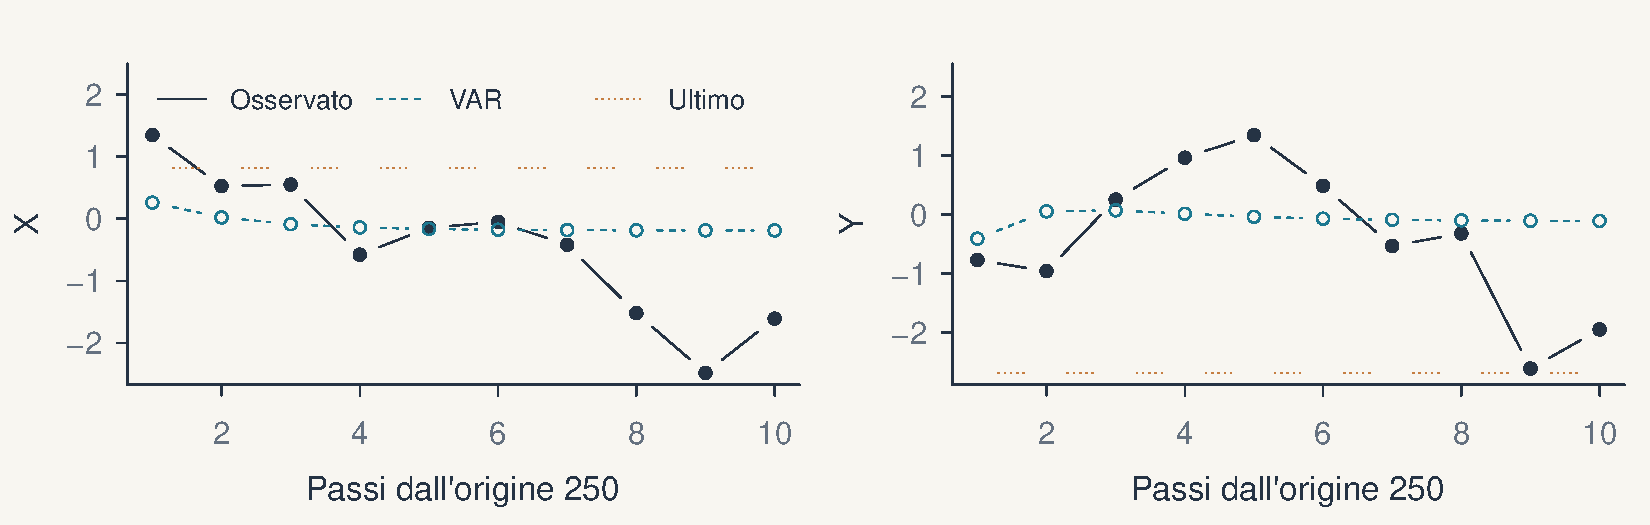
\includegraphics[width=18.05cm,height=5.8cm,keepaspectratio]{Risultati/Figure/32_VAR_previsioni.pdf}
\end{minipage}\end{lrbox}
\typeout{FULLBOX:101:FullWideBox:\the\ht\FullWideBox:\the\dp\FullWideBox}

\begin{lrbox}{\PilotRightBox}
\begin{minipage}[t]{18.1cm}\raggedright\color{Ink}\fontsize{11.3}{14.8}\selectfont
\PBody{Verifica ricorsiva ai tempi 251--260. RMSE X: 1,057 (VAR) e 1,668 (ultimo valore); RMSE Y: 1,193 e 2,561. Dieci tempi descrivono un test breve, non una superiorità generale.}
\end{minipage}\end{lrbox}
\typeout{FULLBOX:101:PilotRightBox:\the\ht\PilotRightBox:\the\dp\PilotRightBox}

\begin{tikzpicture}[remember picture,overlay]
\PilotChrome{Il test VAR conserva due errori e un riferimento}{VIII · SISTEMI MULTIVARIATI}{101}{Un’estensione multivariata deve mostrare il beneficio osservato per ciascuna variabile.}
\node[anchor=north west,inner sep=0] at([xshift=.96cm,yshift=-2.13cm]current page.north west){\usebox{\FullWideBox}};
\node[anchor=north west,inner sep=0] at([xshift=.96cm,yshift=-8.25cm]current page.north west){\usebox{\PilotRightBox}};
\node[anchor=north east,inner sep=0] at([xshift=17.65cm,yshift=-12.06cm]current page.north west){\color{Classical}\fontsize{7.7}{9.2}\selectfont\href{../../03_Notebook_svolti/M10_Futura/M10_N17.html}{M10\_N17 · notebook svolto}};
\end{tikzpicture}\end{frame}

\begin{frame}[plain]\hypertarget{slide102}{}
\bookmark[level=0,page=102]{IX · PROGETTO STATISTICO}
\bookmark[level=1,page=102]{Il progetto parte da una domanda}
\begin{lrbox}{\TitleBox}
\begin{minipage}[t]{17.7cm}\raggedright\color{Ink}\fontsize{11.3}{14.8}\selectfont
\color{Navy}\bfseries\fontsize{20.6}{24.5}\selectfont Il progetto parte da una domanda
\end{minipage}\end{lrbox}
\typeout{FULLBOX:102:TitleBox:\the\ht\TitleBox:\the\dp\TitleBox}

\begin{lrbox}{\RecallBox}
\begin{minipage}[t]{14.3cm}\raggedright\color{Ink}\fontsize{11.3}{14.8}\selectfont
\fontsize{10.3}{13.8}\selectfont Un progetto convincente mantiene allineati domanda, informazione, metodo e criterio di valutazione.
\end{minipage}\end{lrbox}
\typeout{FULLBOX:102:RecallBox:\the\ht\RecallBox:\the\dp\RecallBox}

\begin{lrbox}{\PilotLeftBox}
\begin{minipage}[t]{10.05cm}\raggedright\color{Ink}\fontsize{11.3}{14.8}\selectfont
{\fontsize{10.2}{13.1}\selectfont\renewcommand{\arraystretch}{1.45}\begin{tabular}{@{}p{3.7cm}p{5.4cm}@{}}\toprule
\textbf{Percorso} & \textbf{Domanda verificabile}\\\midrule
Previsione ambientale & Migliora un riferimento a un orizzonte fissato?\\
Morfometria & Una misura disponibile predice un’altra?\\
Struttura dei campioni & Quali raggruppamenti sono stabili e interpretabili?\\
\bottomrule\end{tabular}}
\PInfo{La CO$_2$ guida la lezione. Il progetto di base dei notebook riguarda la morfometria; l’estensione VAR resta facoltativa.}

\end{minipage}\end{lrbox}
\typeout{FULLBOX:102:PilotLeftBox:\the\ht\PilotLeftBox:\the\dp\PilotLeftBox}

\begin{lrbox}{\PilotRightBox}
\begin{minipage}[t]{7.55cm}\raggedright\color{Ink}\fontsize{11.3}{14.8}\selectfont
\PBody{Il progetto integra domanda, dati, metodo, verifica e conclusione. La scelta del metodo segue la quantità da studiare e il modo in cui saranno disponibili i dati.}
\vspace{2.5mm}
\PInfo{Nel clustering manca una risposta futura da prevedere: stabilità e interpretazione dei gruppi richiedono criteri diversi da MAE o RMSE.}
\PSmall{M10\_N10 aiuta a delimitare il progetto; il rapporto evita di includere analisi che non contribuiscono alla domanda.}

\end{minipage}\end{lrbox}
\typeout{FULLBOX:102:PilotRightBox:\the\ht\PilotRightBox:\the\dp\PilotRightBox}

\begin{tikzpicture}[remember picture,overlay]
\PilotChrome{Il progetto parte da una domanda}{IX · PROGETTO STATISTICO}{102}{Un progetto convincente mantiene allineati domanda, informazione, metodo e criterio di valutazione.}
\node[anchor=north west,inner sep=0] at([xshift=.96cm,yshift=-2.13cm]current page.north west){\usebox{\PilotLeftBox}};
\node[anchor=north west,inner sep=0] at([xshift=11.52cm,yshift=-2.13cm]current page.north west){\usebox{\PilotRightBox}};
\node[anchor=north east,inner sep=0] at([xshift=17.65cm,yshift=-12.06cm]current page.north west){\color{Classical}\fontsize{7.7}{9.2}\selectfont\href{../../03_Notebook_svolti/M10_Futura/M10_N10.html}{M10\_N10 · notebook svolto}};
\end{tikzpicture}\end{frame}

\begin{frame}[plain]\hypertarget{slide103}{}
\bookmark[level=1,page=103]{I fossili offrono un secondo compito predittivo}
\begin{lrbox}{\TitleBox}
\begin{minipage}[t]{17.7cm}\raggedright\color{Ink}\fontsize{11.3}{14.8}\selectfont
\color{Navy}\bfseries\fontsize{20.6}{24.5}\selectfont I fossili offrono un secondo compito predittivo
\end{minipage}\end{lrbox}
\typeout{FULLBOX:103:TitleBox:\the\ht\TitleBox:\the\dp\TitleBox}

\begin{lrbox}{\RecallBox}
\begin{minipage}[t]{14.3cm}\raggedright\color{Ink}\fontsize{11.3}{14.8}\selectfont
\fontsize{10.3}{13.8}\selectfont Un secondo caso aiuta a distinguere le regole comuni di previsione dalle caratteristiche del tempo.
\end{minipage}\end{lrbox}
\typeout{FULLBOX:103:RecallBox:\the\ht\RecallBox:\the\dp\RecallBox}

\begin{lrbox}{\PilotLeftBox}
\begin{minipage}[t]{10.05cm}\raggedright\color{Ink}\fontsize{11.3}{14.8}\selectfont
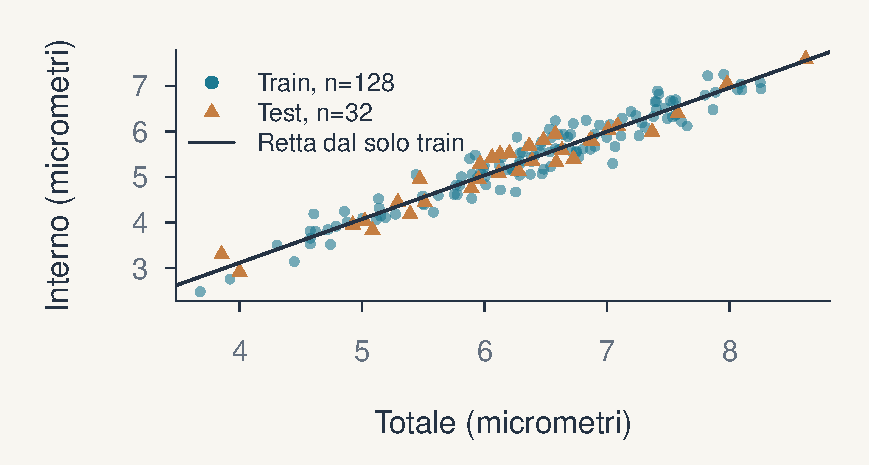
\includegraphics[width=9.85cm,height=5.25cm,keepaspectratio]{Risultati/Figure/26_fossili_train_test.pdf}
\vspace{1.5mm}
\PSmall{Archivio simulato di 160 fossili: 128 per la stima e 32 per il test, una riga su cinque riservata.}

\end{minipage}\end{lrbox}
\typeout{FULLBOX:103:PilotLeftBox:\the\ht\PilotLeftBox:\the\dp\PilotLeftBox}

\begin{lrbox}{\PilotRightBox}
\begin{minipage}[t]{7.55cm}\raggedright\color{Ink}\fontsize{11.3}{14.8}\selectfont
\PBody{Prevediamo il diametro interno dalla misura del diametro totale. Il confronto è fra una retta stimata sul train e la media dei diametri interni del train.}
\vspace{2.5mm}
\PInfo{La separazione deterministica riprende il sito ed è riproducibile. Non equivale a un campionamento indipendente da popolazioni o laboratori nuovi.}
\PCode{R · retta sui fossili simulati}{103_esempio.R}
\end{minipage}\end{lrbox}
\typeout{FULLBOX:103:PilotRightBox:\the\ht\PilotRightBox:\the\dp\PilotRightBox}

\begin{tikzpicture}[remember picture,overlay]
\PilotChrome{I fossili offrono un secondo compito predittivo}{IX · PROGETTO STATISTICO}{103}{Un secondo caso aiuta a distinguere le regole comuni di previsione dalle caratteristiche del tempo.}
\node[anchor=north west,inner sep=0] at([xshift=.96cm,yshift=-2.13cm]current page.north west){\usebox{\PilotLeftBox}};
\node[anchor=north west,inner sep=0] at([xshift=11.52cm,yshift=-2.13cm]current page.north west){\usebox{\PilotRightBox}};
\node[anchor=north east,inner sep=0] at([xshift=17.65cm,yshift=-12.06cm]current page.north west){\color{Classical}\fontsize{7.7}{9.2}\selectfont\href{../../03_Notebook_svolti/M10_Futura/M10_N11.html}{M10\_N11 · notebook svolto}};
\end{tikzpicture}\end{frame}

\begin{frame}[plain]\hypertarget{slide104}{}
\bookmark[level=1,page=104]{La geometria aiuta a prevedere i fossili}
\begin{lrbox}{\TitleBox}
\begin{minipage}[t]{17.7cm}\raggedright\color{Ink}\fontsize{11.3}{14.8}\selectfont
\color{Navy}\bfseries\fontsize{20.6}{24.5}\selectfont La geometria aiuta a prevedere i fossili
\end{minipage}\end{lrbox}
\typeout{FULLBOX:104:TitleBox:\the\ht\TitleBox:\the\dp\TitleBox}

\begin{lrbox}{\RecallBox}
\begin{minipage}[t]{14.3cm}\raggedright\color{Ink}\fontsize{11.3}{14.8}\selectfont
\fontsize{10.3}{13.8}\selectfont Un risultato accurato deve essere interpretato alla luce di come i dati sono stati costruiti.
\end{minipage}\end{lrbox}
\typeout{FULLBOX:104:RecallBox:\the\ht\RecallBox:\the\dp\RecallBox}

\begin{lrbox}{\PilotLeftBox}
\begin{minipage}[t]{10.05cm}\raggedright\color{Ink}\fontsize{11.3}{14.8}\selectfont
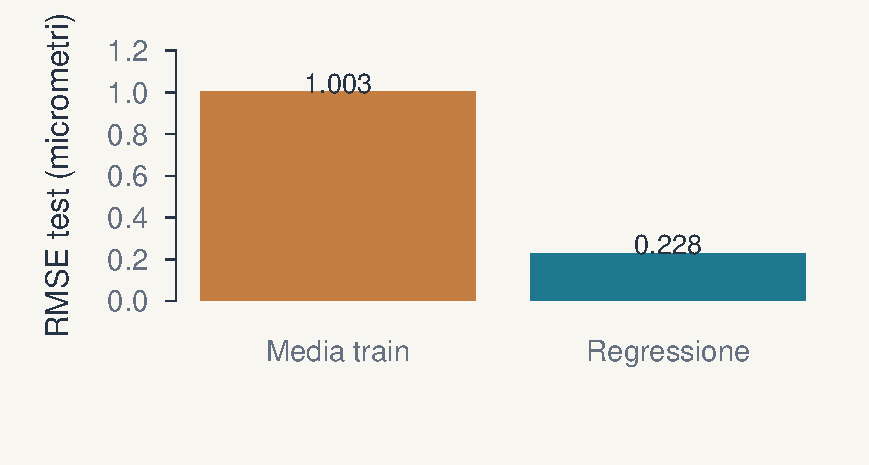
\includegraphics[width=9.85cm,height=4.7cm,keepaspectratio]{Risultati/Figure/29_fossili_RMSE.pdf}
\vspace{1.5mm}
\PSmall{RMSE sul test di 32 fossili, in micrometri; confronto con la media del train.}
\[d_{\mathrm{interno}}=d_{\mathrm{totale}}-2s\]

\end{minipage}\end{lrbox}
\typeout{FULLBOX:104:PilotLeftBox:\the\ht\PilotLeftBox:\the\dp\PilotLeftBox}

\begin{lrbox}{\PilotRightBox}
\begin{minipage}[t]{7.55cm}\raggedright\color{Ink}\fontsize{11.3}{14.8}\selectfont
\PBody{La retta ottiene RMSE 0,228 µm; la media del train 1,003 µm. L’archivio rispetta un’identità geometrica fra diametri e spessore.}
\vspace{2.5mm}
\PInfo{Il risultato è quindi coerente con il generatore. Non costituisce una scoperta biologica su fossili reali.}
\PSmall{Rapporto interno/totale o spessore possono rivelare direttamente la risposta: la loro disponibilità va definita prima del modello.}

\end{minipage}\end{lrbox}
\typeout{FULLBOX:104:PilotRightBox:\the\ht\PilotRightBox:\the\dp\PilotRightBox}

\begin{tikzpicture}[remember picture,overlay]
\PilotChrome{La geometria aiuta a prevedere i fossili}{IX · PROGETTO STATISTICO}{104}{Un risultato accurato deve essere interpretato alla luce di come i dati sono stati costruiti.}
\node[anchor=north west,inner sep=0] at([xshift=.96cm,yshift=-2.13cm]current page.north west){\usebox{\PilotLeftBox}};
\node[anchor=north west,inner sep=0] at([xshift=11.52cm,yshift=-2.13cm]current page.north west){\usebox{\PilotRightBox}};
\node[anchor=north east,inner sep=0] at([xshift=17.65cm,yshift=-12.06cm]current page.north west){\color{Classical}\fontsize{7.7}{9.2}\selectfont\href{../../03_Notebook_svolti/M10_Futura/M10_N11.html}{M10\_N11 · notebook svolto}};
\end{tikzpicture}\end{frame}

\begin{frame}[plain]\hypertarget{slide105}{}
\bookmark[level=1,page=105]{Residui e diagonale completano la metrica}
\begin{lrbox}{\TitleBox}
\begin{minipage}[t]{17.7cm}\raggedright\color{Ink}\fontsize{11.3}{14.8}\selectfont
\color{Navy}\bfseries\fontsize{20.6}{24.5}\selectfont Residui e diagonale completano la metrica
\end{minipage}\end{lrbox}
\typeout{FULLBOX:105:TitleBox:\the\ht\TitleBox:\the\dp\TitleBox}

\begin{lrbox}{\RecallBox}
\begin{minipage}[t]{14.3cm}\raggedright\color{Ink}\fontsize{11.3}{14.8}\selectfont
\fontsize{10.3}{13.8}\selectfont Un numero di prestazione va accompagnato da grafici che rendano visibili direzione e struttura dell’errore.
\end{minipage}\end{lrbox}
\typeout{FULLBOX:105:RecallBox:\the\ht\RecallBox:\the\dp\RecallBox}

\begin{lrbox}{\PilotLeftBox}
\begin{minipage}[t]{10.05cm}\raggedright\color{Ink}\fontsize{11.3}{14.8}\selectfont
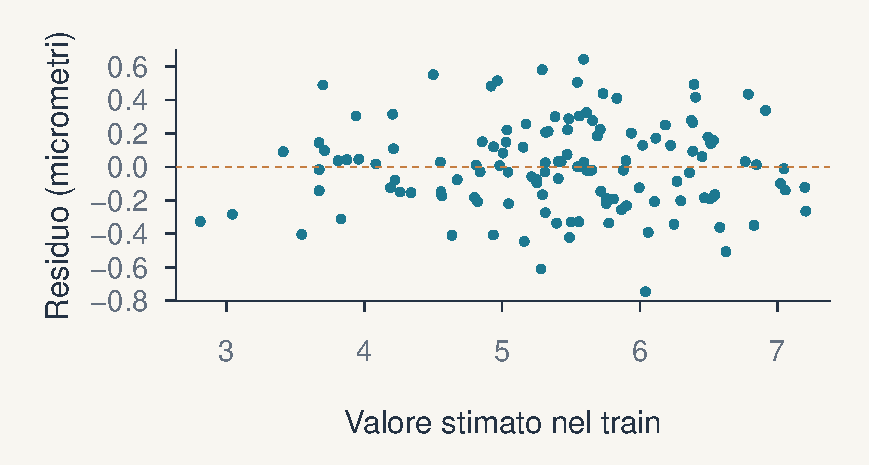
\includegraphics[width=9.85cm,height=5.25cm,keepaspectratio]{Risultati/Figure/28_fossili_residui.pdf}
\vspace{1.5mm}
\PSmall{Residui del modello sul train: controllare andamento e dispersione rispetto ai valori adattati.}

\end{minipage}\end{lrbox}
\typeout{FULLBOX:105:PilotLeftBox:\the\ht\PilotLeftBox:\the\dp\PilotLeftBox}

\begin{lrbox}{\PilotRightBox}
\begin{minipage}[t]{7.55cm}\raggedright\color{Ink}\fontsize{11.3}{14.8}\selectfont
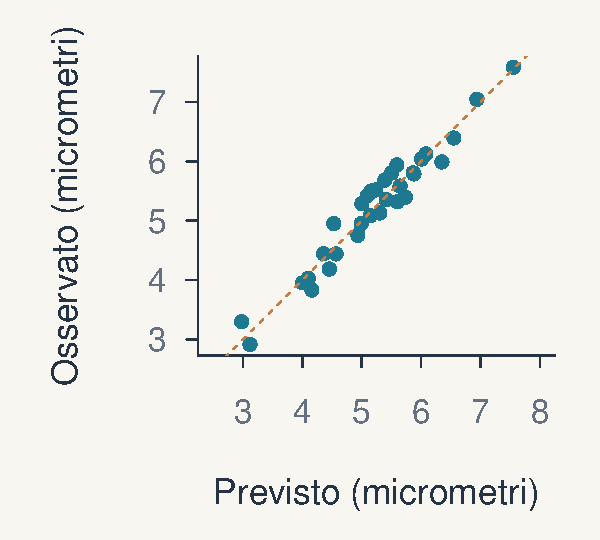
\includegraphics[width=7.4cm,height=3.45cm,keepaspectratio]{Risultati/Figure/27_fossili_osservato_previsto.pdf}
\PBody{Nel test, la diagonale indica previsione perfetta. Scostamenti sistematici possono essere poco visibili in una sola RMSE.}
\vspace{2.5mm}
\PInfo{Il modello usa soltanto il diametro totale. Le proprietà del generatore delimitano l’interpretazione scientifica.}

\end{minipage}\end{lrbox}
\typeout{FULLBOX:105:PilotRightBox:\the\ht\PilotRightBox:\the\dp\PilotRightBox}

\begin{tikzpicture}[remember picture,overlay]
\PilotChrome{Residui e diagonale completano la metrica}{IX · PROGETTO STATISTICO}{105}{Un numero di prestazione va accompagnato da grafici che rendano visibili direzione e struttura dell’errore.}
\node[anchor=north west,inner sep=0] at([xshift=.96cm,yshift=-2.13cm]current page.north west){\usebox{\PilotLeftBox}};
\node[anchor=north west,inner sep=0] at([xshift=11.52cm,yshift=-2.13cm]current page.north west){\usebox{\PilotRightBox}};
\node[anchor=north east,inner sep=0] at([xshift=17.65cm,yshift=-12.06cm]current page.north west){\color{Classical}\fontsize{7.7}{9.2}\selectfont\href{../../03_Notebook_svolti/M10_Futura/M10_N12.html}{M10\_N12 · notebook svolto}};
\end{tikzpicture}\end{frame}

\begin{frame}[plain]\hypertarget{slide106}{}
\bookmark[level=1,page=106]{Una relazione sostenuta dai risultati}
\begin{lrbox}{\TitleBox}
\begin{minipage}[t]{17.7cm}\raggedright\color{Ink}\fontsize{11.3}{14.8}\selectfont
\color{Navy}\bfseries\fontsize{20.6}{24.5}\selectfont Una relazione sostenuta dai risultati
\end{minipage}\end{lrbox}
\typeout{FULLBOX:106:TitleBox:\the\ht\TitleBox:\the\dp\TitleBox}

\begin{lrbox}{\RecallBox}
\begin{minipage}[t]{14.3cm}\raggedright\color{Ink}\fontsize{11.3}{14.8}\selectfont
\fontsize{10.3}{13.8}\selectfont Una conclusione forte è precisa sul risultato e precisa sui suoi limiti.
\end{minipage}\end{lrbox}
\typeout{FULLBOX:106:RecallBox:\the\ht\RecallBox:\the\dp\RecallBox}

\begin{lrbox}{\PilotLeftBox}
\begin{minipage}[t]{10.05cm}\raggedright\color{Ink}\fontsize{11.3}{14.8}\selectfont
{\fontsize{10.2}{13.1}\selectfont\renewcommand{\arraystretch}{1.45}\begin{tabular}{@{}p{2.6cm}p{6.4cm}@{}}\toprule
\textbf{Parte} & \textbf{Contenuto richiesto}\\\midrule
Domanda & Variabile, popolazione o periodo, uso previsto\\
Dati & Fonte, unità, esclusioni e disponibilità\\
Metodo & Ipotesi, riferimenti e scelte\\
Verifica & Disegno, metriche e diagnostica\\
Conclusione & Risposta alla domanda e limiti osservati\\
\bottomrule\end{tabular}}

\end{minipage}\end{lrbox}
\typeout{FULLBOX:106:PilotLeftBox:\the\ht\PilotLeftBox:\the\dp\PilotLeftBox}

\begin{lrbox}{\PilotRightBox}
\begin{minipage}[t]{7.55cm}\raggedright\color{Ink}\fontsize{11.3}{14.8}\selectfont
\PBody{Una conclusione sul caso guida può affermare che il SARIMA migliora i riferimenti nei 36 mesi riservati, con un bias di -0,968 ppm in convenzione osservato meno previsto.}
\vspace{2.5mm}
\PInfo{Va aggiunto che 36 valori coperti non dimostrano calibrazione e che il test riguarda una sola origine storica.}
\PSmall{M10\_N13 costruisce il testo usando i risultati realmente calcolati.}

\end{minipage}\end{lrbox}
\typeout{FULLBOX:106:PilotRightBox:\the\ht\PilotRightBox:\the\dp\PilotRightBox}

\begin{tikzpicture}[remember picture,overlay]
\PilotChrome{Una relazione sostenuta dai risultati}{IX · PROGETTO STATISTICO}{106}{Una conclusione forte è precisa sul risultato e precisa sui suoi limiti.}
\node[anchor=north west,inner sep=0] at([xshift=.96cm,yshift=-2.13cm]current page.north west){\usebox{\PilotLeftBox}};
\node[anchor=north west,inner sep=0] at([xshift=11.52cm,yshift=-2.13cm]current page.north west){\usebox{\PilotRightBox}};
\node[anchor=north east,inner sep=0] at([xshift=17.65cm,yshift=-12.06cm]current page.north west){\color{Classical}\fontsize{7.7}{9.2}\selectfont\href{../../03_Notebook_svolti/M10_Futura/M10_N13.html}{M10\_N13 · notebook svolto}};
\end{tikzpicture}\end{frame}

\begin{frame}[plain]\hypertarget{slide107}{}
\bookmark[level=1,page=107]{Esportare numeri, date e provenienza}
\begin{lrbox}{\TitleBox}
\begin{minipage}[t]{17.7cm}\raggedright\color{Ink}\fontsize{11.3}{14.8}\selectfont
\color{Navy}\bfseries\fontsize{20.6}{24.5}\selectfont Esportare numeri, date e provenienza
\end{minipage}\end{lrbox}
\typeout{FULLBOX:107:TitleBox:\the\ht\TitleBox:\the\dp\TitleBox}

\begin{lrbox}{\RecallBox}
\begin{minipage}[t]{14.3cm}\raggedright\color{Ink}\fontsize{11.3}{14.8}\selectfont
\fontsize{10.3}{13.8}\selectfont Un file riutilizzabile deve conservare il significato delle colonne insieme ai valori.
\end{minipage}\end{lrbox}
\typeout{FULLBOX:107:RecallBox:\the\ht\RecallBox:\the\dp\RecallBox}

\begin{lrbox}{\PilotLeftBox}
\begin{minipage}[t]{10.05cm}\raggedright\color{Ink}\fontsize{11.3}{14.8}\selectfont
{\fontsize{10.2}{13.1}\selectfont\renewcommand{\arraystretch}{1.45}\begin{tabular}{@{}p{2.4cm}p{6.7cm}@{}}\toprule
\textbf{File} & \textbf{Contenuto}\\\midrule
CSV & Date, osservato, previsto, errore e bande\\
RDS & Oggetti stimati per riprendere il lavoro\\
R / Rmd & Procedura leggibile ed eseguibile\\
HTML / PDF & Risultato consultabile senza esecuzione\\
Metadati & Versioni, fonti e impronte dei file\\
\bottomrule\end{tabular}}

\end{minipage}\end{lrbox}
\typeout{FULLBOX:107:PilotLeftBox:\the\ht\PilotLeftBox:\the\dp\PilotLeftBox}

\begin{lrbox}{\PilotRightBox}
\begin{minipage}[t]{7.55cm}\raggedright\color{Ink}\fontsize{11.3}{14.8}\selectfont
\PBody{I file hanno nomi stabili e percorsi relativi al progetto. Una tabella esportata non deve perdere l’origine della previsione o l’orientamento dell’errore.}
\vspace{2.5mm}
\PInfo{M10\_N19 controlla duplicati e integrità delle chiavi; M10\_N09 prepara l’esportazione dei risultati.}
\PCode{R · tabella pronta per l’esportazione}{107_esempio.R}
\end{minipage}\end{lrbox}
\typeout{FULLBOX:107:PilotRightBox:\the\ht\PilotRightBox:\the\dp\PilotRightBox}

\begin{tikzpicture}[remember picture,overlay]
\PilotChrome{Esportare numeri, date e provenienza}{IX · PROGETTO STATISTICO}{107}{Un file riutilizzabile deve conservare il significato delle colonne insieme ai valori.}
\node[anchor=north west,inner sep=0] at([xshift=.96cm,yshift=-2.13cm]current page.north west){\usebox{\PilotLeftBox}};
\node[anchor=north west,inner sep=0] at([xshift=11.52cm,yshift=-2.13cm]current page.north west){\usebox{\PilotRightBox}};
\node[anchor=north east,inner sep=0] at([xshift=17.65cm,yshift=-12.06cm]current page.north west){\color{Classical}\fontsize{7.7}{9.2}\selectfont\href{../../03_Notebook_svolti/M10_Futura/M10_N19.html}{M10\_N19 · notebook svolto}};
\end{tikzpicture}\end{frame}

\begin{frame}[plain]\hypertarget{slide108}{}
\bookmark[level=1,page=108]{La consegna deve funzionare da una cartella pulita}
\begin{lrbox}{\TitleBox}
\begin{minipage}[t]{17.7cm}\raggedright\color{Ink}\fontsize{11.3}{14.8}\selectfont
\color{Navy}\bfseries\fontsize{20.6}{24.5}\selectfont La consegna deve funzionare da una cartella pulita
\end{minipage}\end{lrbox}
\typeout{FULLBOX:108:TitleBox:\the\ht\TitleBox:\the\dp\TitleBox}

\begin{lrbox}{\RecallBox}
\begin{minipage}[t]{14.3cm}\raggedright\color{Ink}\fontsize{11.3}{14.8}\selectfont
\fontsize{10.3}{13.8}\selectfont Un risultato riproducibile può essere ricostruito e interpretato senza dipendere dalla memoria dell’autore.
\end{minipage}\end{lrbox}
\typeout{FULLBOX:108:RecallBox:\the\ht\RecallBox:\the\dp\RecallBox}

\begin{lrbox}{\PilotLeftBox}
\begin{minipage}[t]{10.05cm}\raggedright\color{Ink}\fontsize{11.3}{14.8}\selectfont
\PLabel{Quattro prove di riproducibilità}
{\fontsize{10.2}{13.1}\selectfont\renewcommand{\arraystretch}{1.45}\begin{tabular}{@{}p{3.4cm}p{5.7cm}@{}}\toprule
\textbf{Prova} & \textbf{Evidenza da conservare}\\\midrule
Riesecuzione & Log e versione di R\\
Dati locali & Nessun download implicito\\
Coerenza numerica & Tabelle e figure dagli stessi calcoli\\
Integrità & Manifest SHA-256 e file richiesti\\
\bottomrule\end{tabular}}

\end{minipage}\end{lrbox}
\typeout{FULLBOX:108:PilotLeftBox:\the\ht\PilotLeftBox:\the\dp\PilotLeftBox}

\begin{lrbox}{\PilotRightBox}
\begin{minipage}[t]{7.55cm}\raggedright\color{Ink}\fontsize{11.3}{14.8}\selectfont
\PBody{Il progetto contiene dati, codice, risultati e istruzioni. Il notebook HTML permette la lettura offline; il Rmd conserva il percorso per ripetere il lavoro.}
\vspace{2.5mm}
\PInfo{Una verifica dei file non sostituisce la valutazione scientifica. Completa il controllo di formule, unità, date e conclusioni.}
\PSmall{M10\_N18 accompagna la consegna. Il pacchetto include gli esiti delle esecuzioni svolte per questa edizione.}

\end{minipage}\end{lrbox}
\typeout{FULLBOX:108:PilotRightBox:\the\ht\PilotRightBox:\the\dp\PilotRightBox}

\begin{tikzpicture}[remember picture,overlay]
\PilotChrome{La consegna deve funzionare da una cartella pulita}{IX · PROGETTO STATISTICO}{108}{Un risultato riproducibile può essere ricostruito e interpretato senza dipendere dalla memoria dell’autore.}
\node[anchor=north west,inner sep=0] at([xshift=.96cm,yshift=-2.13cm]current page.north west){\usebox{\PilotLeftBox}};
\node[anchor=north west,inner sep=0] at([xshift=11.52cm,yshift=-2.13cm]current page.north west){\usebox{\PilotRightBox}};
\node[anchor=north east,inner sep=0] at([xshift=17.65cm,yshift=-12.06cm]current page.north west){\color{Classical}\fontsize{7.7}{9.2}\selectfont\href{../../03_Notebook_svolti/M10_Futura/M10_N18.html}{M10\_N18 · notebook svolto}};
\end{tikzpicture}\end{frame}

\begin{frame}[plain]\hypertarget{slide109}{}
\bookmark[level=1,page=109]{Riferimenti per teoria, software e dati}
\begin{lrbox}{\TitleBox}
\begin{minipage}[t]{17.7cm}\raggedright\color{Ink}\fontsize{11.3}{14.8}\selectfont
\color{Navy}\bfseries\fontsize{20.6}{24.5}\selectfont Riferimenti per teoria, software e dati
\end{minipage}\end{lrbox}
\typeout{FULLBOX:109:TitleBox:\the\ht\TitleBox:\the\dp\TitleBox}

\begin{lrbox}{\RecallBox}
\begin{minipage}[t]{14.3cm}\raggedright\color{Ink}\fontsize{11.3}{14.8}\selectfont
\fontsize{10.3}{13.8}\selectfont Le fonti rendono verificabili sia le scelte teoriche sia le convenzioni del calcolo.
\end{minipage}\end{lrbox}
\typeout{FULLBOX:109:RecallBox:\the\ht\RecallBox:\the\dp\RecallBox}

\begin{lrbox}{\PilotLeftBox}
\begin{minipage}[t]{10.05cm}\raggedright\color{Ink}\fontsize{11.3}{14.8}\selectfont
\PLabel{Fonti primarie e documentazione}
\PBody{Hyndman e Athanasopoulos, \emph{Forecasting: Principles and Practice}, 3ª edizione: riferimenti, errori, validazione temporale, ARIMA e intervalli.}
\vspace{2.5mm}
\PSmall{\href{https://otexts.com/fpp3/}{otexts.com/fpp3/}}
\PBody{R Core Team, documentazione di stats: arima, predict.Arima, Box.test, ARMAacf, ARMAtoMA, lm e anova.}
\vspace{2.5mm}
\PSmall{\href{https://stat.ethz.ch/R-manual/R-devel/library/stats/html/arima.html}{Manuale R: arima} · \href{https://stat.ethz.ch/R-manual/R-devel/library/stats/html/predict.arima.html}{predict.Arima} · \href{https://stat.ethz.ch/R-manual/R-devel/library/stats/html/box.test.html}{Box.test}}

\end{minipage}\end{lrbox}
\typeout{FULLBOX:109:PilotLeftBox:\the\ht\PilotLeftBox:\the\dp\PilotLeftBox}

\begin{lrbox}{\PilotRightBox}
\begin{minipage}[t]{7.55cm}\raggedright\color{Ink}\fontsize{11.3}{14.8}\selectfont
\PBody{GeoStat Lab, modulo M10 e laboratori M10\_N01--M10\_N20: programma, convenzioni e specifica centrale.}
\vspace{2.5mm}
\PSmall{\href{https://marzione00.github.io/Lab_Geo/percorso/M10.html}{Modulo M10 sul sito}}
\PInfo{Dati locali: CO$_2$ storica da M09, fossili simulati da M07, processi simulati da M09. Fonti, hash e dettagli sono in FONTI\_E\_NOTE.md e Dati/PROVENIENZA.json.}
\PSmall{Snapshot del sito: 20 novembre 2026. Revisione identificata nei metadati del pacchetto.}

\end{minipage}\end{lrbox}
\typeout{FULLBOX:109:PilotRightBox:\the\ht\PilotRightBox:\the\dp\PilotRightBox}

\begin{tikzpicture}[remember picture,overlay]
\PilotChrome{Riferimenti per teoria, software e dati}{IX · PROGETTO STATISTICO}{109}{Le fonti rendono verificabili sia le scelte teoriche sia le convenzioni del calcolo.}
\node[anchor=north west,inner sep=0] at([xshift=.96cm,yshift=-2.13cm]current page.north west){\usebox{\PilotLeftBox}};
\node[anchor=north west,inner sep=0] at([xshift=11.52cm,yshift=-2.13cm]current page.north west){\usebox{\PilotRightBox}};
\end{tikzpicture}\end{frame}

\begin{frame}[plain]\hypertarget{slide110}{}
\bookmark[level=1,page=110]{Prevedere, discutere, ricostruire}
\begin{lrbox}{\TitleBox}
\begin{minipage}[t]{17.7cm}\raggedright\color{Ink}\fontsize{11.3}{14.8}\selectfont
\color{Navy}\bfseries\fontsize{20.6}{24.5}\selectfont Prevedere, discutere, ricostruire
\end{minipage}\end{lrbox}
\typeout{FULLBOX:110:TitleBox:\the\ht\TitleBox:\the\dp\TitleBox}

\begin{lrbox}{\RecallBox}
\begin{minipage}[t]{14.3cm}\raggedright\color{Ink}\fontsize{11.3}{14.8}\selectfont
\fontsize{10.3}{13.8}\selectfont Prevedere significa rendere esplicito ciò che sappiamo, misurare gli errori e motivare ciò che concludiamo.
\end{minipage}\end{lrbox}
\typeout{FULLBOX:110:RecallBox:\the\ht\RecallBox:\the\dp\RecallBox}

\begin{lrbox}{\PilotLeftBox}
\begin{minipage}[t]{10.05cm}\raggedright\color{Ink}\fontsize{11.3}{14.8}\selectfont
\PLabel{Criteri per valutare il progetto}
{\fontsize{10.2}{13.1}\selectfont\renewcommand{\arraystretch}{1.45}\begin{tabular}{@{}p{3.6cm}p{5.5cm}@{}}\toprule
\textbf{Criterio} & \textbf{Evidenza osservabile}\\\midrule
Domanda chiara & Quantità e uso della previsione espliciti\\
Metodo coerente & Ipotesi e riferimenti motivati\\
Verifica corretta & Separazione dei dati e metriche adeguate\\
Interpretazione & Risultati collegati alla domanda\\
Riproducibilità & Dati, codice, fonti e istruzioni completi\\
\bottomrule\end{tabular}}

\end{minipage}\end{lrbox}
\typeout{FULLBOX:110:PilotLeftBox:\the\ht\PilotLeftBox:\the\dp\PilotLeftBox}

\begin{lrbox}{\PilotRightBox}
\begin{minipage}[t]{7.55cm}\raggedright\color{Ink}\fontsize{11.3}{14.8}\selectfont
\PBody{Il progetto conclude il percorso unendo descrizione, modello e verifica. La complessità aggiunta deve produrre informazione utile e comprensibile.}
\vspace{2.5mm}
\PInfo{Prima della consegna: un’altra persona può capire la domanda, ripetere i calcoli e individuare quali conclusioni sono sostenute dai dati?}
\PSmall{\href{https://marzione00.github.io/Lab_Geo/\#indice}{Indice del corso} · \hyperlink{slide2}{Indice di Futura}}

\end{minipage}\end{lrbox}
\typeout{FULLBOX:110:PilotRightBox:\the\ht\PilotRightBox:\the\dp\PilotRightBox}

\begin{tikzpicture}[remember picture,overlay]
\PilotChrome{Prevedere, discutere, ricostruire}{IX · PROGETTO STATISTICO}{110}{Prevedere significa rendere esplicito ciò che sappiamo, misurare gli errori e motivare ciò che concludiamo.}
\node[anchor=north west,inner sep=0] at([xshift=.96cm,yshift=-2.13cm]current page.north west){\usebox{\PilotLeftBox}};
\node[anchor=north west,inner sep=0] at([xshift=11.52cm,yshift=-2.13cm]current page.north west){\usebox{\PilotRightBox}};
\node[anchor=north east,inner sep=0] at([xshift=17.65cm,yshift=-12.06cm]current page.north west){\color{Classical}\fontsize{7.7}{9.2}\selectfont\href{../../03_Notebook_svolti/M10_Futura/M10_N18.html}{M10\_N18 · notebook svolto}};
\end{tikzpicture}\end{frame}

\end{document}
